\documentclass[twoside]{book}

% Packages required by doxygen
\usepackage{fixltx2e}
\usepackage{calc}
\usepackage{doxygen}
\usepackage[export]{adjustbox} % also loads graphicx
\usepackage{graphicx}
\usepackage[utf8]{inputenc}
\usepackage{makeidx}
\usepackage{multicol}
\usepackage{multirow}
\PassOptionsToPackage{warn}{textcomp}
\usepackage{textcomp}
\usepackage[nointegrals]{wasysym}
\usepackage[table]{xcolor}

% Font selection
\usepackage[T1]{fontenc}
\usepackage[scaled=.90]{helvet}
\usepackage{courier}
\usepackage{amssymb}
\usepackage{sectsty}
\renewcommand{\familydefault}{\sfdefault}
\allsectionsfont{%
  \fontseries{bc}\selectfont%
  \color{darkgray}%
}
\renewcommand{\DoxyLabelFont}{%
  \fontseries{bc}\selectfont%
  \color{darkgray}%
}
\newcommand{\+}{\discretionary{\mbox{\scriptsize$\hookleftarrow$}}{}{}}

% Page & text layout
\usepackage{geometry}
\geometry{%
  a4paper,%
  top=2.5cm,%
  bottom=2.5cm,%
  left=2.5cm,%
  right=2.5cm%
}
\tolerance=750
\hfuzz=15pt
\hbadness=750
\setlength{\emergencystretch}{15pt}
\setlength{\parindent}{0cm}
\setlength{\parskip}{3ex plus 2ex minus 2ex}
\makeatletter
\renewcommand{\paragraph}{%
  \@startsection{paragraph}{4}{0ex}{-1.0ex}{1.0ex}{%
    \normalfont\normalsize\bfseries\SS@parafont%
  }%
}
\renewcommand{\subparagraph}{%
  \@startsection{subparagraph}{5}{0ex}{-1.0ex}{1.0ex}{%
    \normalfont\normalsize\bfseries\SS@subparafont%
  }%
}
\makeatother

% Headers & footers
\usepackage{fancyhdr}
\pagestyle{fancyplain}
\fancyhead[LE]{\fancyplain{}{\bfseries\thepage}}
\fancyhead[CE]{\fancyplain{}{}}
\fancyhead[RE]{\fancyplain{}{\bfseries\leftmark}}
\fancyhead[LO]{\fancyplain{}{\bfseries\rightmark}}
\fancyhead[CO]{\fancyplain{}{}}
\fancyhead[RO]{\fancyplain{}{\bfseries\thepage}}
\fancyfoot[LE]{\fancyplain{}{}}
\fancyfoot[CE]{\fancyplain{}{}}
\fancyfoot[RE]{\fancyplain{}{\bfseries\scriptsize Generated by Doxygen }}
\fancyfoot[LO]{\fancyplain{}{\bfseries\scriptsize Generated by Doxygen }}
\fancyfoot[CO]{\fancyplain{}{}}
\fancyfoot[RO]{\fancyplain{}{}}
\renewcommand{\footrulewidth}{0.4pt}
\renewcommand{\chaptermark}[1]{%
  \markboth{#1}{}%
}
\renewcommand{\sectionmark}[1]{%
  \markright{\thesection\ #1}%
}

% Indices & bibliography
\usepackage{natbib}
\usepackage[titles]{tocloft}
\setcounter{tocdepth}{3}
\setcounter{secnumdepth}{5}
\makeindex

% Hyperlinks (required, but should be loaded last)
\usepackage{ifpdf}
\ifpdf
  \usepackage[pdftex,pagebackref=true]{hyperref}
\else
  \usepackage[ps2pdf,pagebackref=true]{hyperref}
\fi
\hypersetup{%
  colorlinks=true,%
  linkcolor=blue,%
  citecolor=blue,%
  unicode%
}

% Custom commands
\newcommand{\clearemptydoublepage}{%
  \newpage{\pagestyle{empty}\cleardoublepage}%
}

\usepackage{caption}
\captionsetup{labelsep=space,justification=centering,font={bf},singlelinecheck=off,skip=4pt,position=top}

%===== C O N T E N T S =====

\begin{document}

% Titlepage & ToC
\hypersetup{pageanchor=false,
             bookmarksnumbered=true,
             pdfencoding=unicode
            }
\pagenumbering{roman}
\begin{titlepage}
\vspace*{7cm}
\begin{center}%
{\Large Super\+Goose\+\_\+64 \\[1ex]\large Version 1.\+0 }\\
\vspace*{1cm}
{\large Generated by Doxygen 1.8.11}\\
\end{center}
\end{titlepage}
\clearemptydoublepage
\tableofcontents
\clearemptydoublepage
\pagenumbering{arabic}
\hypersetup{pageanchor=true}

%--- Begin generated contents ---
\chapter{Main Page}
\label{index}\hypertarget{index}{}\hypertarget{index_intro_sec}{}\section{Super\+Goose\+\_\+64}\label{index_intro_sec}
Welcome to our incredible game! Please, have fun while playing it and remember to ask the creators if you have any doubts. Cheers \+:)\hypertarget{index_install_sec}{}\section{The creators}\label{index_install_sec}
\hypertarget{index_step1}{}\subsection{Eric Morales\+:}\label{index_step1}
\begin{DoxyVerb}eric.morales@estudiante.uam.es
\end{DoxyVerb}
\hypertarget{index_step2}{}\subsection{Victor Yrazusta\+:}\label{index_step2}
\begin{DoxyVerb}victor.yrazusta@estudiante.uam.es
\end{DoxyVerb}
\hypertarget{index_step3}{}\subsection{Alejandro Pascual\+:}\label{index_step3}
\begin{DoxyVerb}alejandro.pascualp@estudiante.uam.es
\end{DoxyVerb}
\hypertarget{index_step4}{}\subsection{Javier Lougedo\+:}\label{index_step4}
\begin{DoxyVerb}javier.lougedo@estudiante.uam.es\end{DoxyVerb}
 
\chapter{Test List}
\label{test}
\hypertarget{test}{}

\begin{DoxyRefList}
\item[\label{test__test000001}%
\hypertarget{test__test000001}{}%
Member \hyperlink{command__test_8h_abed44af325fd42a3f4f4aa134315435c}{test1\+\_\+command\+\_\+create} ()]Test command creation  
\item[\label{test__test000002}%
\hypertarget{test__test000002}{}%
Member \hyperlink{command__test_8h_aadf731a98e5122e70ede7cdc68ba621f}{test1\+\_\+command\+\_\+destroy} ()]Test command destruction  
\item[\label{test__test000007}%
\hypertarget{test__test000007}{}%
Member \hyperlink{command__test_8h_aa5f2c4937af80de245778a8ac348cf3b}{test1\+\_\+command\+\_\+get\+\_\+command} ()]Test command for reading command-\/$>$command setting  
\item[\label{test__test000009}%
\hypertarget{test__test000009}{}%
Member \hyperlink{command__test_8h_a6aa58960e0653f7a4fb5c30350d64e54}{test1\+\_\+command\+\_\+get\+\_\+info} ()]Test command for reading command-\/$>$info setting  
\item[\label{test__test000004}%
\hypertarget{test__test000004}{}%
Member \hyperlink{command__test_8h_a932afa8fb63c9b8ba551d030886ce491}{test1\+\_\+command\+\_\+get\+\_\+user\+\_\+input} ()]Test command input  
\item[\label{test__test000085}%
\hypertarget{test__test000085}{}%
Member \hyperlink{game__test_8h_ab936ab03dff02b8edde97651f12384ea}{test1\+\_\+game\+\_\+add\+\_\+link} ()]Test with normal conditions  
\item[\label{test__test000047}%
\hypertarget{test__test000047}{}%
Member \hyperlink{game__test_8h_ac60415277fc72d0a231b17e482a6609b}{test1\+\_\+game\+\_\+add\+\_\+object} ()]Test to see if adding objects normally works correctly  
\item[\label{test__test000042}%
\hypertarget{test__test000042}{}%
Member \hyperlink{game__test_8h_a4adb115e4624c38738c938b999f6c949}{test1\+\_\+game\+\_\+add\+\_\+player} ()]Test with normal conditions  
\item[\label{test__test000038}%
\hypertarget{test__test000038}{}%
Member \hyperlink{game__test_8h_a49b59f8e75a8a4375c98ded865f16fcc}{test1\+\_\+game\+\_\+add\+\_\+space} ()]Test to see if adding spaces works correctly  
\item[\label{test__test000027}%
\hypertarget{test__test000027}{}%
Member \hyperlink{game__test_8h_a1d5c70cf073b025bb5d74413cecd929b}{test1\+\_\+game\+\_\+create} ()]Test to see if game\+\_\+create works correctly  
\item[\label{test__test000028}%
\hypertarget{test__test000028}{}%
Member \hyperlink{game__test_8h_a867d2e7bebdfa55ee8b8a73764c46f5b}{test1\+\_\+game\+\_\+create\+\_\+from\+\_\+file} ()]Test to check if a game is created correctly from a file.  
\item[\label{test__test000034}%
\hypertarget{test__test000034}{}%
Member \hyperlink{game__test_8h_abb9b53b5dbd1f36a9518e11c0a0bee16}{test1\+\_\+game\+\_\+destroy} ()]Test if game destroys a created Game.  
\item[\label{test__test000067}%
\hypertarget{test__test000067}{}%
Member \hyperlink{game__test_8h_a6c4aa8df2680e65915e1c9b687164028}{test1\+\_\+game\+\_\+find} ()]Test to see if it works normally  
\item[\label{test__test000070}%
\hypertarget{test__test000070}{}%
Member \hyperlink{game__test_8h_acf41e567400a66fca3a2c1224aa44de9}{test1\+\_\+game\+\_\+find\+\_\+name} ()]Test to see if it works normally  
\item[\label{test__test000065}%
\hypertarget{test__test000065}{}%
Member \hyperlink{game__test_8h_a7d3e65d6960a38ca883d0591a679f9c4}{test1\+\_\+game\+\_\+get\+\_\+dies\+\_\+number} ()]Test to see if the number (0) of returned dies is correct.  
\item[\label{test__test000082}%
\hypertarget{test__test000082}{}%
Member \hyperlink{game__test_8h_a979cf97b28d14da099d77631877101ef}{test1\+\_\+game\+\_\+get\+\_\+last\+\_\+check} ()]Test to see if works in normal conditions with an object  
\item[\label{test__test000078}%
\hypertarget{test__test000078}{}%
Member \hyperlink{game__test_8h_adffc2120d97aef04f9387431397defbc}{test1\+\_\+game\+\_\+get\+\_\+last\+\_\+command} ()]Test to see if works in normal conditions  
\item[\label{test__test000061}%
\hypertarget{test__test000061}{}%
Member \hyperlink{game__test_8h_a1649f86f3414e97a09b230bae2b9911b}{test1\+\_\+game\+\_\+get\+\_\+objects\+\_\+number} ()]Test to see if the number (1) of returned objects is correct.  
\item[\label{test__test000057}%
\hypertarget{test__test000057}{}%
Member \hyperlink{game__test_8h_af8bec2d2267ab511ba4c3d0a3fa46622}{test1\+\_\+game\+\_\+get\+\_\+players\+\_\+number} ()]Test to see if the number (1) of returned players is correct.  
\item[\label{test__test000053}%
\hypertarget{test__test000053}{}%
Member \hyperlink{game__test_8h_ab8c2b4ef2ac2319b3d039e3775f6ce34}{test1\+\_\+game\+\_\+get\+\_\+spaces\+\_\+number} ()]Test to see if the number (1) of returned spaces is correct.  
\item[\label{test__test000080}%
\hypertarget{test__test000080}{}%
Member \hyperlink{game__test_8h_a2eb3d363edd323ead30c8392366e2fa9}{test1\+\_\+game\+\_\+get\+\_\+status\+\_\+last\+\_\+command} ()]Test to see if works in normal conditions  
\item[\label{test__test000036}%
\hypertarget{test__test000036}{}%
Member \hyperlink{game__test_8h_a6ab3378c3e627b8ff5cb397ecb46d268}{test1\+\_\+game\+\_\+is\+\_\+over} ()]Test if normally a created Game is over or not  
\item[\label{test__test000023}%
\hypertarget{test__test000023}{}%
Member \hyperlink{game__reader__test_8h_aed14cf4de40dd313470f6f609e62e918}{test1\+\_\+game\+\_\+reader\+\_\+load\+\_\+links} ()]Test function for loading Links  
\item[\label{test__test000019}%
\hypertarget{test__test000019}{}%
Member \hyperlink{game__reader__test_8h_a28e7be804609ddfdf00b4798e5256030}{test1\+\_\+game\+\_\+reader\+\_\+load\+\_\+objects} ()]Test function for loading Objects  
\item[\label{test__test000015}%
\hypertarget{test__test000015}{}%
Member \hyperlink{game__reader__test_8h_a1f978e0818495ddc5008be23a38e5995}{test1\+\_\+game\+\_\+reader\+\_\+load\+\_\+players} ()]Test function for loading Players  
\item[\label{test__test000011}%
\hypertarget{test__test000011}{}%
Member \hyperlink{game__reader__test_8h_a99136dde4243bfa5eaf03ef9c2716ffe}{test1\+\_\+game\+\_\+reader\+\_\+load\+\_\+spaces} ()]Test function for loading Spaces  
\item[\label{test__test000073}%
\hypertarget{test__test000073}{}%
Member \hyperlink{game__test_8h_a467fe2bad25b7d53fa51ad3901f4672f}{test1\+\_\+game\+\_\+set\+\_\+object\+\_\+location} ()]Test to see if it works normally 

Test to see if it lets us move an object normally  
\item[\label{test__test000032}%
\hypertarget{test__test000032}{}%
Member \hyperlink{game__test_8h_acef689d23c451c738aab116984001501}{test1\+\_\+game\+\_\+update} ()]Test if game updates with a N\+U\+LL Game (simple, but is easy to see if game update isnt working)  
\item[\label{test__test000093}%
\hypertarget{test__test000093}{}%
Member \hyperlink{inventory__test_8h_ae81ec4669af03331ca8a228567736474}{test1\+\_\+inventory\+\_\+add} ()]Test function for adding an object  
\item[\label{test__test000114}%
\hypertarget{test__test000114}{}%
Member \hyperlink{inventory__test_8h_a94926e4449b777046515a173637bee84}{test1\+\_\+inventory\+\_\+check\+\_\+object} ()]Test function for checking if an Object Id is in the Inventory  
\item[\label{test__test000089}%
\hypertarget{test__test000089}{}%
Member \hyperlink{inventory__test_8h_a33638f1a88ae16ab8d6bee00145b82b8}{test1\+\_\+inventory\+\_\+create} ()]Test function for inventory creation  
\item[\label{test__test000097}%
\hypertarget{test__test000097}{}%
Member \hyperlink{inventory__test_8h_a0198822eb71da7d7e1a8742e6953c82c}{test1\+\_\+inventory\+\_\+del} ()]Test function for deleting an object  
\item[\label{test__test000091}%
\hypertarget{test__test000091}{}%
Member \hyperlink{inventory__test_8h_ab161eafe6a61db39b2237e97c677d822}{test1\+\_\+inventory\+\_\+destroy} ()]Test function for inventory destruction  
\item[\label{test__test000111}%
\hypertarget{test__test000111}{}%
Member \hyperlink{inventory__test_8h_a17c5d7d6ecb4161696deca0155e13f4f}{test1\+\_\+inventory\+\_\+get\+\_\+max\+\_\+objects} ()]Test function for getting the capacity  
\item[\label{test__test000105}%
\hypertarget{test__test000105}{}%
Member \hyperlink{inventory__test_8h_a7feab32c68817ece1716946f02738dc5}{test1\+\_\+inventory\+\_\+get\+\_\+object\+\_\+id} ()]Test function for getting an Object Id  
\item[\label{test__test000108}%
\hypertarget{test__test000108}{}%
Member \hyperlink{inventory__test_8h_a03ef2e867bad9b096df6047fcb22331e}{test1\+\_\+inventory\+\_\+get\+\_\+objects\+\_\+number} ()]Test function for getting the current number of Objects Ids  
\item[\label{test__test000117}%
\hypertarget{test__test000117}{}%
Member \hyperlink{inventory__test_8h_afe8c9730e30b58535afc0481970ab2b1}{test1\+\_\+inventory\+\_\+is\+\_\+empty} ()]Test function for checking if the Inventory is empty  
\item[\label{test__test000120}%
\hypertarget{test__test000120}{}%
Member \hyperlink{inventory__test_8h_a7eb3ba387e33c42ff45331c9d9aada34}{test1\+\_\+inventory\+\_\+is\+\_\+full} ()]Test function for checking if the Inventory is full  
\item[\label{test__test000101}%
\hypertarget{test__test000101}{}%
Member \hyperlink{inventory__test_8h_aedc895d6409678b2176d822c105c3796}{test1\+\_\+inventory\+\_\+set\+\_\+max\+\_\+objects} ()]Test function for setting the capacity  
\item[\label{test__test000130}%
\hypertarget{test__test000130}{}%
Member \hyperlink{link__test_8h_af84ec726ff74021eff3ccc9c3116a634}{test1\+\_\+link\+\_\+add\+\_\+space} ()]Test function for link-\/$>$space1 and link-\/$>$space2 settings  
\item[\label{test__test000123}%
\hypertarget{test__test000123}{}%
Member \hyperlink{link__test_8h_a82c5ee441ad22caad8272212a9e9cc26}{test1\+\_\+link\+\_\+create} ()]Test link creation  
\item[\label{test__test000144}%
\hypertarget{test__test000144}{}%
Member \hyperlink{link__test_8h_ad4ca02e93472a080362a005ea4840218}{test1\+\_\+link\+\_\+destroy} ()]Test function for destroying links  
\item[\label{test__test000135}%
\hypertarget{test__test000135}{}%
Member \hyperlink{link__test_8h_a19c70f79fd51d123173f7aaf6ae50bf8}{test1\+\_\+link\+\_\+get\+\_\+id} ()]Test function for reading link-\/$>$id setting  
\item[\label{test__test000137}%
\hypertarget{test__test000137}{}%
Member \hyperlink{link__test_8h_a044128db00a5cc385d7157dea8bdf3c3}{test1\+\_\+link\+\_\+get\+\_\+name} ()]Test function for reading link-\/$>$name setting  
\item[\label{test__test000141}%
\hypertarget{test__test000141}{}%
Member \hyperlink{link__test_8h_a342f65b583bf77b00715e4f76c63c84f}{test1\+\_\+link\+\_\+get\+\_\+other\+\_\+side} ()]Test function for link\+\_\+get\+\_\+other\+\_\+side  
\item[\label{test__test000139}%
\hypertarget{test__test000139}{}%
Member \hyperlink{link__test_8h_a9f7bf73b9398d551c64f6c845e9e1560}{test1\+\_\+link\+\_\+get\+\_\+status} ()]Test function for reading link-\/$>$status setting  
\item[\label{test__test000127}%
\hypertarget{test__test000127}{}%
Member \hyperlink{link__test_8h_ae0e478a0540bed26befc071591e3ff6c}{test1\+\_\+link\+\_\+set\+\_\+name} ()]Test function for link-\/$>$name setting  
\item[\label{test__test000133}%
\hypertarget{test__test000133}{}%
Member \hyperlink{link__test_8h_a3b39fdba0c3c967716572bfb01beec27}{test1\+\_\+link\+\_\+set\+\_\+status} ()]Test function for link-\/$>$status setting  
\item[\label{test__test000146}%
\hypertarget{test__test000146}{}%
Member \hyperlink{object__test_8h_a3836d69f92ce7149d56bafcaec83f516}{test1\+\_\+object\+\_\+create} ()]Test object creation  
\item[\label{test__test000162}%
\hypertarget{test__test000162}{}%
Member \hyperlink{object__test_8h_a73c676e5d625179d75b96eed035a0876}{test1\+\_\+object\+\_\+get\+\_\+check} ()]Test to see if the created object returns the correct description  
\item[\label{test__test000158}%
\hypertarget{test__test000158}{}%
Member \hyperlink{object__test_8h_aa88e9e9dab92ba9c58851d7a7a8415f0}{test1\+\_\+object\+\_\+get\+\_\+id} ()]Test to see if Object has the given Id  
\item[\label{test__test000160}%
\hypertarget{test__test000160}{}%
Member \hyperlink{object__test_8h_ac62fbd4db0970e9942aa900a3ee2bba4}{test1\+\_\+object\+\_\+get\+\_\+location} ()]Test to see if the created object returns the correct location  
\item[\label{test__test000156}%
\hypertarget{test__test000156}{}%
Member \hyperlink{object__test_8h_ad2411bc3cc47c9905e63a3d9c561d369}{test1\+\_\+object\+\_\+get\+\_\+name} ()]Test to see if Object has the given name  
\item[\label{test__test000154}%
\hypertarget{test__test000154}{}%
Member \hyperlink{object__test_8h_a7e652e4dcf897db42363f6098bc1c3da}{test1\+\_\+object\+\_\+set\+\_\+check} ()]Test function for set check in normal conditions  
\item[\label{test__test000151}%
\hypertarget{test__test000151}{}%
Member \hyperlink{object__test_8h_aeed901e95aa669185059c85183e68a24}{test1\+\_\+object\+\_\+set\+\_\+location} ()]Test function for object set location in normal conditions  
\item[\label{test__test000148}%
\hypertarget{test__test000148}{}%
Member \hyperlink{object__test_8h_a74e25ad653c4a32b9922fff8e4f916fd}{test1\+\_\+object\+\_\+set\+\_\+name} ()]Test function for object name setting  
\item[\label{test__test000189}%
\hypertarget{test__test000189}{}%
Member \hyperlink{player__test_8h_a14a3e4867e2ad3287c8efa99cd36904e}{test1\+\_\+player\+\_\+add\+\_\+object} ()]Test if objects are added properly onto the player  
\item[\label{test__test000201}%
\hypertarget{test__test000201}{}%
Member \hyperlink{player__test_8h_a95396b550249d790fe55be1e553517ae}{test1\+\_\+player\+\_\+check\+\_\+object} ()]Test to see if the check object works on a Player with an object  
\item[\label{test__test000164}%
\hypertarget{test__test000164}{}%
Member \hyperlink{player__test_8h_ab29768452373e16bb6aaa1f7998f62fb}{test1\+\_\+player\+\_\+create} ()]Test player creation  
\item[\label{test__test000191}%
\hypertarget{test__test000191}{}%
Member \hyperlink{player__test_8h_ab8680555a9d30950ffa0547011a0f787}{test1\+\_\+player\+\_\+del\+\_\+object} ()]Test if objects are deleted properly into the player  
\item[\label{test__test000179}%
\hypertarget{test__test000179}{}%
Member \hyperlink{player__test_8h_a07beea3b974453e5d8001d04e6db5ac4}{test1\+\_\+player\+\_\+get\+\_\+graphic\+\_\+description} ()]Test to see if the created player with the given graphic description returns the given graphic description  
\item[\label{test__test000177}%
\hypertarget{test__test000177}{}%
Member \hyperlink{player__test_8h_a790a75dc179c00c60c784d3e34c0e5aa}{test1\+\_\+player\+\_\+get\+\_\+id} ()]Test to see if Player has the given Id  
\item[\label{test__test000187}%
\hypertarget{test__test000187}{}%
Member \hyperlink{player__test_8h_a408a557a0cff748c10fb9a03445af191}{test1\+\_\+player\+\_\+get\+\_\+location} ()]Test if the location Id of the player is OK  
\item[\label{test__test000175}%
\hypertarget{test__test000175}{}%
Member \hyperlink{player__test_8h_a94068667d8faa66a4ad293dd2c60f2ef}{test1\+\_\+player\+\_\+get\+\_\+name} ()]Test to see if Player has the given name  
\item[\label{test__test000181}%
\hypertarget{test__test000181}{}%
Member \hyperlink{player__test_8h_a53eb6ee101f01fe988c5da03129d2e2f}{test1\+\_\+player\+\_\+get\+\_\+object} ()]Test to see if a Player has the given Object on its inventory.  
\item[\label{test__test000183}%
\hypertarget{test__test000183}{}%
Member \hyperlink{player__test_8h_af1b1a4517ec347b3b953c9fc9b3ea1a5}{test1\+\_\+player\+\_\+get\+\_\+objects\+\_\+number} ()]Test to see if player carried objects number is correct  
\item[\label{test__test000194}%
\hypertarget{test__test000194}{}%
Member \hyperlink{player__test_8h_a9e7594fd2a1016abea94e0b88016d6ec}{test1\+\_\+player\+\_\+is\+\_\+empty} ()]Test if a created Id is empty  
\item[\label{test__test000197}%
\hypertarget{test__test000197}{}%
Member \hyperlink{player__test_8h_a2c7a96147ce996da70dce4b4cb37ecef}{test1\+\_\+player\+\_\+is\+\_\+full} ()]Test if a player with all the objects possible is or not full  
\item[\label{test__test000169}%
\hypertarget{test__test000169}{}%
Member \hyperlink{player__test_8h_adfd8f1d4fd7d500f9b5236db4e697ea3}{test1\+\_\+player\+\_\+set\+\_\+graphic\+\_\+description} ()]Test graphic description of a player setting  
\item[\label{test__test000172}%
\hypertarget{test__test000172}{}%
Member \hyperlink{player__test_8h_aec6799a4f46c3f3c471fcb668addcad4}{test1\+\_\+player\+\_\+set\+\_\+location} ()]Test in normal conditions for the location setting  
\item[\label{test__test000166}%
\hypertarget{test__test000166}{}%
Member \hyperlink{player__test_8h_a9d87c09e6af910d695265e3fd77ae3a2}{test1\+\_\+player\+\_\+set\+\_\+name} ()]Test function for player name setting  
\item[\label{test__test000245}%
\hypertarget{test__test000245}{}%
Member \hyperlink{space__test_8h_afe51f379fb29f8e96f9f034df991de30}{test1\+\_\+space\+\_\+add\+\_\+object} ()]Test if objects are added properly onto the space  
\item[\label{test__test000254}%
\hypertarget{test__test000254}{}%
Member \hyperlink{space__test_8h_a6989d8b8621fd8374ae4c0109591943c}{test1\+\_\+space\+\_\+check\+\_\+object} ()]Test to see if the check object works on a Space with an object  
\item[\label{test__test000204}%
\hypertarget{test__test000204}{}%
Member \hyperlink{space__test_8h_a69278cc022dc5688d4725f8d36317b30}{test1\+\_\+space\+\_\+create} ()]Test space creation  
\item[\label{test__test000237}%
\hypertarget{test__test000237}{}%
Member \hyperlink{space__test_8h_aea5055c002d6150e36f79b3ebe48d07d}{test1\+\_\+space\+\_\+get\+\_\+check} ()]Test to see if the created space with the given check returns the given check  
\item[\label{test__test000231}%
\hypertarget{test__test000231}{}%
Member \hyperlink{space__test_8h_a354adb2722b06ec65b7212d2736d6417}{test1\+\_\+space\+\_\+get\+\_\+east} ()]Test to check if the eastern Id is set and got properly  
\item[\label{test__test000235}%
\hypertarget{test__test000235}{}%
Member \hyperlink{space__test_8h_a4279d034f757a350dcaa9604903b179b}{test1\+\_\+space\+\_\+get\+\_\+graphic\+\_\+description} ()]Test to see if the created space with the given graphic description returns the given graphic description  
\item[\label{test__test000225}%
\hypertarget{test__test000225}{}%
Member \hyperlink{space__test_8h_a920df9e02482f4f1e6a5ebcaec523860}{test1\+\_\+space\+\_\+get\+\_\+id} ()]Test to see if Space has the given Id  
\item[\label{test__test000223}%
\hypertarget{test__test000223}{}%
Member \hyperlink{space__test_8h_ad12c42523c517507566c5c68b1527689}{test1\+\_\+space\+\_\+get\+\_\+name} ()]Test to see if Space has the given name  
\item[\label{test__test000227}%
\hypertarget{test__test000227}{}%
Member \hyperlink{space__test_8h_a3a87f1e1e173d622bfbd3bcd14e060ca}{test1\+\_\+space\+\_\+get\+\_\+north} ()]Test to check if the northern Id is set and got properly  
\item[\label{test__test000239}%
\hypertarget{test__test000239}{}%
Member \hyperlink{space__test_8h_ab47960fac6126d77d7b3d163177bbd4f}{test1\+\_\+space\+\_\+get\+\_\+object\+\_\+id} ()]Test to see if the Id of an object on a Space is the one the Space returns.  
\item[\label{test__test000241}%
\hypertarget{test__test000241}{}%
Member \hyperlink{space__test_8h_a99dcb9ec68282e5488ea34997a213783}{test1\+\_\+space\+\_\+get\+\_\+objects\+\_\+number} ()]Test if Space carries one object  
\item[\label{test__test000229}%
\hypertarget{test__test000229}{}%
Member \hyperlink{space__test_8h_a8e345065f58565e131bdb3a9d0096ed5}{test1\+\_\+space\+\_\+get\+\_\+south} ()]Test to check if the southern Id is set and got properly  
\item[\label{test__test000233}%
\hypertarget{test__test000233}{}%
Member \hyperlink{space__test_8h_a1f08c6866885bfc093717f57b1b86539}{test1\+\_\+space\+\_\+get\+\_\+west} ()]Test to check if the western Id is set and got properly  
\item[\label{test__test000247}%
\hypertarget{test__test000247}{}%
Member \hyperlink{space__test_8h_af6acddb4ba70ed941100be42d8f40b38}{test1\+\_\+space\+\_\+is\+\_\+empty} ()]Test if a created Id is empty  
\item[\label{test__test000250}%
\hypertarget{test__test000250}{}%
Member \hyperlink{space__test_8h_a9b23efa95cd3c18574cc8c1ef83ae7a9}{test1\+\_\+space\+\_\+is\+\_\+full} ()]Test if a space with all the objects possible is or not full  
\item[\label{test__test000220}%
\hypertarget{test__test000220}{}%
Member \hyperlink{space__test_8h_adedb9f74b100fba85454e4f2b4aca122}{test1\+\_\+space\+\_\+set\+\_\+check} ()]Test check of a space setting  
\item[\label{test__test000213}%
\hypertarget{test__test000213}{}%
Member \hyperlink{space__test_8h_ab1f093af4be3ca8e525d0517cc846f47}{test1\+\_\+space\+\_\+set\+\_\+east} ()]Test function for east Id setting  
\item[\label{test__test000217}%
\hypertarget{test__test000217}{}%
Member \hyperlink{space__test_8h_ad8b51e7da141d7a3b29039a9a1d83013}{test1\+\_\+space\+\_\+set\+\_\+graphic\+\_\+description} ()]Test graphic description of a space setting  
\item[\label{test__test000206}%
\hypertarget{test__test000206}{}%
Member \hyperlink{space__test_8h_a2569bab6cfeec15f722d232bb8c78c9e}{test1\+\_\+space\+\_\+set\+\_\+name} ()]Test function for space\+\_\+name setting  
\item[\label{test__test000209}%
\hypertarget{test__test000209}{}%
Member \hyperlink{space__test_8h_a3d3457a89f705948102cf1e5d4a7b45b}{test1\+\_\+space\+\_\+set\+\_\+north} ()]Test function for north Id setting  
\item[\label{test__test000211}%
\hypertarget{test__test000211}{}%
Member \hyperlink{space__test_8h_a21938e16547b3080e9251f960117a859}{test1\+\_\+space\+\_\+set\+\_\+south} ()]Test function for south Id setting  
\item[\label{test__test000215}%
\hypertarget{test__test000215}{}%
Member \hyperlink{space__test_8h_ab680a8797f793dffd58546074b87d21f}{test1\+\_\+space\+\_\+set\+\_\+west} ()]Test function for west Id setting  
\item[\label{test__test000003}%
\hypertarget{test__test000003}{}%
Member \hyperlink{command__test_8h_ad445f3e81035d4ab32ebc1526eb83fcb}{test2\+\_\+command\+\_\+destroy} ()]Test command destruction  
\item[\label{test__test000008}%
\hypertarget{test__test000008}{}%
Member \hyperlink{command__test_8h_a9c9d95687224d936e9486c0421969411}{test2\+\_\+command\+\_\+get\+\_\+command} ()]Test command for reading command-\/$>$command setting  
\item[\label{test__test000010}%
\hypertarget{test__test000010}{}%
Member \hyperlink{command__test_8h_a057697416fb8f5d97d82f18b5f231930}{test2\+\_\+command\+\_\+get\+\_\+info} ()]Test command for reading command-\/$>$info setting  
\item[\label{test__test000005}%
\hypertarget{test__test000005}{}%
Member \hyperlink{command__test_8h_a3ba7658db8aa069706b344d42ceabfaa}{test2\+\_\+command\+\_\+get\+\_\+user\+\_\+input} ()]Test command input  
\item[\label{test__test000086}%
\hypertarget{test__test000086}{}%
Member \hyperlink{game__test_8h_af5c4dd79b2a7b67adbeeb8df5791a5de}{test2\+\_\+game\+\_\+add\+\_\+link} ()]Test with N\+U\+LL game  
\item[\label{test__test000048}%
\hypertarget{test__test000048}{}%
Member \hyperlink{game__test_8h_ab996895e69c5d41fab5515e88aed3975}{test2\+\_\+game\+\_\+add\+\_\+object} ()]Test to see if adding objects doesn\textquotesingle{}t work for N\+U\+LL games  
\item[\label{test__test000043}%
\hypertarget{test__test000043}{}%
Member \hyperlink{game__test_8h_a42bb53c500bf8ae4dce0e144a85cd80b}{test2\+\_\+game\+\_\+add\+\_\+player} ()]Test with N\+U\+LL game  
\item[\label{test__test000039}%
\hypertarget{test__test000039}{}%
Member \hyperlink{game__test_8h_aed0f40f3ab1c252e548b038542d7409d}{test2\+\_\+game\+\_\+add\+\_\+space} ()]Test to see if adding spaces doesn\textquotesingle{}t work for N\+U\+LL games  
\item[\label{test__test000029}%
\hypertarget{test__test000029}{}%
Member \hyperlink{game__test_8h_ad6ce67f6184f6ead2aaca860f64e9b76}{test2\+\_\+game\+\_\+create\+\_\+from\+\_\+file} ()]Test to check if it works with a N\+U\+LL game  
\item[\label{test__test000035}%
\hypertarget{test__test000035}{}%
Member \hyperlink{game__test_8h_a91a33a9fce738616f2140d06a6ff079f}{test2\+\_\+game\+\_\+destroy} ()]Test if game destroys a N\+U\+LL Game  
\item[\label{test__test000068}%
\hypertarget{test__test000068}{}%
Member \hyperlink{game__test_8h_a5894e9abe6b633d53b01ad8691655a26}{test2\+\_\+game\+\_\+find} ()]Test to see if it works with a N\+U\+LL Game  
\item[\label{test__test000071}%
\hypertarget{test__test000071}{}%
Member \hyperlink{game__test_8h_a4a26a36f14da83a296ff5057ddfd67a7}{test2\+\_\+game\+\_\+find\+\_\+name} ()]Test to see if it works with a N\+U\+LL Game  
\item[\label{test__test000066}%
\hypertarget{test__test000066}{}%
Member \hyperlink{game__test_8h_a3cf79c20d8101232319754300c699a22}{test2\+\_\+game\+\_\+get\+\_\+dies\+\_\+number} ()]Test to see the number of dies in a N\+U\+LL game.  
\item[\label{test__test000083}%
\hypertarget{test__test000083}{}%
Member \hyperlink{game__test_8h_af601b07387856d9fbf5fb30eaae11191}{test2\+\_\+game\+\_\+get\+\_\+last\+\_\+check} ()]Test to see how it works with a N\+U\+LL Game  
\item[\label{test__test000079}%
\hypertarget{test__test000079}{}%
Member \hyperlink{game__test_8h_ac6463a36d0a06d720225b64f894ec445}{test2\+\_\+game\+\_\+get\+\_\+last\+\_\+command} ()]Test with N\+U\+LL Game  
\item[\label{test__test000062}%
\hypertarget{test__test000062}{}%
Member \hyperlink{game__test_8h_a666e45de68b2bbc214dbd1c7f0cbc1ff}{test2\+\_\+game\+\_\+get\+\_\+objects\+\_\+number} ()]Test to see if the number (0) of returned objects is correct.  
\item[\label{test__test000058}%
\hypertarget{test__test000058}{}%
Member \hyperlink{game__test_8h_a2a530a4de5f42cebd34d3a2b13b571b3}{test2\+\_\+game\+\_\+get\+\_\+players\+\_\+number} ()]Test to see if the number (0) of returned players is correct.  
\item[\label{test__test000054}%
\hypertarget{test__test000054}{}%
Member \hyperlink{game__test_8h_ae8acea54aeabc7ca6bb3f4ccb7019947}{test2\+\_\+game\+\_\+get\+\_\+spaces\+\_\+number} ()]Test to see if the number (0) of returned spaces is correct.  
\item[\label{test__test000081}%
\hypertarget{test__test000081}{}%
Member \hyperlink{game__test_8h_a5828e75b146cd90e87938d17f5c0c114}{test2\+\_\+game\+\_\+get\+\_\+status\+\_\+last\+\_\+command} ()]Test to see if works with a N\+U\+LL Game  
\item[\label{test__test000037}%
\hypertarget{test__test000037}{}%
Member \hyperlink{game__test_8h_aad6c50be5f1d541ca5414b86558ef422}{test2\+\_\+game\+\_\+is\+\_\+over} ()]Test if a N\+U\+LL game is over  
\item[\label{test__test000024}%
\hypertarget{test__test000024}{}%
Member \hyperlink{game__reader__test_8h_a7366cf536491c6f3be1145b0d7b2b32c}{test2\+\_\+game\+\_\+reader\+\_\+load\+\_\+links} ()]Test function for loading Links  
\item[\label{test__test000020}%
\hypertarget{test__test000020}{}%
Member \hyperlink{game__reader__test_8h_a5bd7d88df7ebba1510197eafd63a4ca3}{test2\+\_\+game\+\_\+reader\+\_\+load\+\_\+objects} ()]Test function for loading Objects  
\item[\label{test__test000016}%
\hypertarget{test__test000016}{}%
Member \hyperlink{game__reader__test_8h_a2a92d2c5944de5ec790969ade0d10c8b}{test2\+\_\+game\+\_\+reader\+\_\+load\+\_\+players} ()]Test function for loading Players  
\item[\label{test__test000012}%
\hypertarget{test__test000012}{}%
Member \hyperlink{game__reader__test_8h_a1bf200d01046a242ee3379e62545fa01}{test2\+\_\+game\+\_\+reader\+\_\+load\+\_\+spaces} ()]Test function for loading Spaces  
\item[\label{test__test000074}%
\hypertarget{test__test000074}{}%
Member \hyperlink{game__test_8h_a2bee8c4494438aa5cdc301ca6ef40e88}{test2\+\_\+game\+\_\+set\+\_\+object\+\_\+location} ()]Test to see if it works with N\+U\+LL games  
\item[\label{test__test000033}%
\hypertarget{test__test000033}{}%
Member \hyperlink{game__test_8h_aa7c7e1467a24f4d1086096b73a38739e}{test2\+\_\+game\+\_\+update} ()]Test if game updates without a command (simple, but is easy to see if game update isnt working)  
\item[\label{test__test000094}%
\hypertarget{test__test000094}{}%
Member \hyperlink{inventory__test_8h_a48019cb45cb5918233d5d42334d2be17}{test2\+\_\+inventory\+\_\+add} ()]Test function for adding an object  
\item[\label{test__test000115}%
\hypertarget{test__test000115}{}%
Member \hyperlink{inventory__test_8h_a847aa346d12ebb77d86d202bd0fa99b6}{test2\+\_\+inventory\+\_\+check\+\_\+object} ()]Test function for checking if an Object Id is in the Inventory  
\item[\label{test__test000090}%
\hypertarget{test__test000090}{}%
Member \hyperlink{inventory__test_8h_a73a6080c360a8870c4ffc734e989c8b3}{test2\+\_\+inventory\+\_\+create} ()]Test function for inventory creation  
\item[\label{test__test000098}%
\hypertarget{test__test000098}{}%
Member \hyperlink{inventory__test_8h_a242baf98676c3685d4696ec6c006cbb9}{test2\+\_\+inventory\+\_\+del} ()]Test function for deleting an object  
\item[\label{test__test000092}%
\hypertarget{test__test000092}{}%
Member \hyperlink{inventory__test_8h_a9f3daec28c696c0671e6a3e905359741}{test2\+\_\+inventory\+\_\+destroy} ()]Test function for inventory destruction  
\item[\label{test__test000112}%
\hypertarget{test__test000112}{}%
Member \hyperlink{inventory__test_8h_ac75954611acab583f780145532ab3197}{test2\+\_\+inventory\+\_\+get\+\_\+max\+\_\+objects} ()]Test function for getting the capacity  
\item[\label{test__test000106}%
\hypertarget{test__test000106}{}%
Member \hyperlink{inventory__test_8h_a41ba2562e1c60e222110f05c9a8e221e}{test2\+\_\+inventory\+\_\+get\+\_\+object\+\_\+id} ()]Test function for getting an Object Id  
\item[\label{test__test000109}%
\hypertarget{test__test000109}{}%
Member \hyperlink{inventory__test_8h_a3546785f0cda504b4d16c89c19f0b23e}{test2\+\_\+inventory\+\_\+get\+\_\+objects\+\_\+number} ()]Test function for getting the current number of Objects Ids  
\item[\label{test__test000118}%
\hypertarget{test__test000118}{}%
Member \hyperlink{inventory__test_8h_a4d2a2a4d4ba59446d013debfe9bf05dc}{test2\+\_\+inventory\+\_\+is\+\_\+empty} ()]Test function for checking if the Inventory is empty  
\item[\label{test__test000121}%
\hypertarget{test__test000121}{}%
Member \hyperlink{inventory__test_8h_a1c9e567d4919d5aaccc9580815a8a81d}{test2\+\_\+inventory\+\_\+is\+\_\+full} ()]Test function for checking if the Inventory is full  
\item[\label{test__test000102}%
\hypertarget{test__test000102}{}%
Member \hyperlink{inventory__test_8h_aff93a7fb7ffbac1890ce563012a9d372}{test2\+\_\+inventory\+\_\+set\+\_\+max\+\_\+objects} ()]Test function for setting the capacity  
\item[\label{test__test000131}%
\hypertarget{test__test000131}{}%
Member \hyperlink{link__test_8h_a1a9f0d8d05848f9cc3f9f30097ca9452}{test2\+\_\+link\+\_\+add\+\_\+space} ()]Test function for link-\/$>$space1 and link-\/$>$space2 settings  
\item[\label{test__test000124}%
\hypertarget{test__test000124}{}%
Member \hyperlink{link__test_8h_a24b5463da176c3e578b0a0fa8bb1f9f0}{test2\+\_\+link\+\_\+create} ()]Test link creation  
\item[\label{test__test000145}%
\hypertarget{test__test000145}{}%
Member \hyperlink{link__test_8h_afae7294e1213cade145448511cfae536}{test2\+\_\+link\+\_\+destroy} ()]Test function for destroying links  
\item[\label{test__test000136}%
\hypertarget{test__test000136}{}%
Member \hyperlink{link__test_8h_a0f967a1782dd7264e73ad428d22d125d}{test2\+\_\+link\+\_\+get\+\_\+id} ()]Test function for reading link-\/$>$id setting  
\item[\label{test__test000138}%
\hypertarget{test__test000138}{}%
Member \hyperlink{link__test_8h_a4efc6cfcdc210e2803f9d285734c571e}{test2\+\_\+link\+\_\+get\+\_\+name} ()]Test function for reading link-\/$>$name setting  
\item[\label{test__test000142}%
\hypertarget{test__test000142}{}%
Member \hyperlink{link__test_8h_a9bb64e905b519d629239c31029ec4cd2}{test2\+\_\+link\+\_\+get\+\_\+other\+\_\+side} ()]Test function for link\+\_\+get\+\_\+other\+\_\+side  
\item[\label{test__test000140}%
\hypertarget{test__test000140}{}%
Member \hyperlink{link__test_8h_a7d1062febd832b21e69df5f071425b4c}{test2\+\_\+link\+\_\+get\+\_\+status} ()]Test function for reading link-\/$>$status setting  
\item[\label{test__test000128}%
\hypertarget{test__test000128}{}%
Member \hyperlink{link__test_8h_aa66c1e991620a5a758ba6e4d6b4a8b73}{test2\+\_\+link\+\_\+set\+\_\+name} ()]Test function for link-\/$>$name setting  
\item[\label{test__test000134}%
\hypertarget{test__test000134}{}%
Member \hyperlink{link__test_8h_a315ea19cd24434d2153b5df9f372a561}{test2\+\_\+link\+\_\+set\+\_\+status} ()]Test function for link-\/$>$status setting  
\item[\label{test__test000147}%
\hypertarget{test__test000147}{}%
Member \hyperlink{object__test_8h_add54ab5e33a1b0a93e9ddcf73591bd9f}{test2\+\_\+object\+\_\+create} ()]Test object creation  
\item[\label{test__test000163}%
\hypertarget{test__test000163}{}%
Member \hyperlink{object__test_8h_a0a46a923bd913c88dc697341d19cfb2b}{test2\+\_\+object\+\_\+get\+\_\+check} ()]Test to see if the created object returns the correct description  
\item[\label{test__test000159}%
\hypertarget{test__test000159}{}%
Member \hyperlink{object__test_8h_a1ff250f0f43297f57fcce1f3a6ae490b}{test2\+\_\+object\+\_\+get\+\_\+id} ()]Test to see if a N\+U\+LL Object Id is N\+O\+\_\+\+ID  
\item[\label{test__test000161}%
\hypertarget{test__test000161}{}%
Member \hyperlink{object__test_8h_aa8e3d1f2c80097572d9a453737d8cd44}{test2\+\_\+object\+\_\+get\+\_\+location} ()]Test to see if the created object returns the correct location  
\item[\label{test__test000157}%
\hypertarget{test__test000157}{}%
Member \hyperlink{object__test_8h_abdfafbc7b8588d3dcdb05fd2beb2397e}{test2\+\_\+object\+\_\+get\+\_\+name} ()]Test if getting a name from a N\+U\+LL Object works (it shouldn\textquotesingle{}t)  
\item[\label{test__test000155}%
\hypertarget{test__test000155}{}%
Member \hyperlink{object__test_8h_a16f5685f75ace0aaaeef2b296d64221d}{test2\+\_\+object\+\_\+set\+\_\+check} ()]Test function for set check in abnormal conditions (N\+U\+LL O\+B\+J\+E\+CT)  
\item[\label{test__test000152}%
\hypertarget{test__test000152}{}%
Member \hyperlink{object__test_8h_a552de466dc09eaef60eff5835455fbb6}{test2\+\_\+object\+\_\+set\+\_\+location} ()]Test function for object set location with N\+U\+LL objects  
\item[\label{test__test000149}%
\hypertarget{test__test000149}{}%
Member \hyperlink{object__test_8h_acf42b7e7be91ede243f2aaa56c4c9347}{test2\+\_\+object\+\_\+set\+\_\+name} ()]Test function for object name setting  
\item[\label{test__test000190}%
\hypertarget{test__test000190}{}%
Member \hyperlink{player__test_8h_a864d3935cf61953950b10df0e656306d}{test2\+\_\+player\+\_\+add\+\_\+object} ()]Test if objects adding onto a N\+U\+LL Player works  
\item[\label{test__test000202}%
\hypertarget{test__test000202}{}%
Member \hyperlink{player__test_8h_a18d23e4d24cc31a552f264e270856a49}{test2\+\_\+player\+\_\+check\+\_\+object} ()]Test to see if the check object works on a Player without an object  
\item[\label{test__test000165}%
\hypertarget{test__test000165}{}%
Member \hyperlink{player__test_8h_a4f6eca5f9d8c08d2a7fc70c209ecf854}{test2\+\_\+player\+\_\+create} ()]Test player creation  
\item[\label{test__test000192}%
\hypertarget{test__test000192}{}%
Member \hyperlink{player__test_8h_a32008cea3e74553151b6c8c8ad1b565a}{test2\+\_\+player\+\_\+del\+\_\+object} ()]Test if objects deleting into a N\+U\+LL Player works  
\item[\label{test__test000180}%
\hypertarget{test__test000180}{}%
Member \hyperlink{player__test_8h_a94aa58d9c954a4817ea34ba7d7c17493}{test2\+\_\+player\+\_\+get\+\_\+graphic\+\_\+description} ()]Test to check if the graphic description of a N\+U\+LL Player is N\+U\+LL  
\item[\label{test__test000178}%
\hypertarget{test__test000178}{}%
Member \hyperlink{player__test_8h_a9fa80f0c0e46b45eb9f1685b102a5826}{test2\+\_\+player\+\_\+get\+\_\+id} ()]Test to see if a N\+U\+LL Player Id is N\+O\+\_\+\+ID  
\item[\label{test__test000188}%
\hypertarget{test__test000188}{}%
Member \hyperlink{player__test_8h_a4c5605fac4bd716e1dfb2744db4fa8a1}{test2\+\_\+player\+\_\+get\+\_\+location} ()]Test if the location Id of a N\+U\+LL player is N\+O\+\_\+\+ID  
\item[\label{test__test000176}%
\hypertarget{test__test000176}{}%
Member \hyperlink{player__test_8h_a3aa908fd360b74e7786422260e8e16a0}{test2\+\_\+player\+\_\+get\+\_\+name} ()]Test if getting a name from a N\+U\+LL Player works (it shouldn\textquotesingle{}t)  
\item[\label{test__test000182}%
\hypertarget{test__test000182}{}%
Member \hyperlink{player__test_8h_a83e8fea42cd87151cd67d0643a78134f}{test2\+\_\+player\+\_\+get\+\_\+object} ()]Test to check if a N\+U\+LL Player returns a N\+O\+\_\+\+ID when asked for the object Id  
\item[\label{test__test000184}%
\hypertarget{test__test000184}{}%
Member \hyperlink{player__test_8h_a718933fd0429cdc840c6624882550d3b}{test2\+\_\+player\+\_\+get\+\_\+objects\+\_\+number} ()]Test if Player its generated with 0 objects  
\item[\label{test__test000195}%
\hypertarget{test__test000195}{}%
Member \hyperlink{player__test_8h_ab101e35e3034e348688b0a8ffd81f8ad}{test2\+\_\+player\+\_\+is\+\_\+empty} ()]Test if a N\+U\+LL Player is empty  
\item[\label{test__test000198}%
\hypertarget{test__test000198}{}%
Member \hyperlink{player__test_8h_a2a0781d2fbfb7f0d8870b7501db230a6}{test2\+\_\+player\+\_\+is\+\_\+full} ()]Test if an empty Player is full  
\item[\label{test__test000170}%
\hypertarget{test__test000170}{}%
Member \hyperlink{player__test_8h_a4d18de1dc3a06db35a47aaa2c81df4fd}{test2\+\_\+player\+\_\+set\+\_\+graphic\+\_\+description} ()]Test graphic description setting on a N\+U\+LL Player  
\item[\label{test__test000173}%
\hypertarget{test__test000173}{}%
Member \hyperlink{player__test_8h_a2c702753d9e2e3df9ef4abf2d1b9bc8d}{test2\+\_\+player\+\_\+set\+\_\+location} ()]Test in abnormal conditions for the location setting  
\item[\label{test__test000167}%
\hypertarget{test__test000167}{}%
Member \hyperlink{player__test_8h_a6e7ce8ff791f4bf63749df647a44263f}{test2\+\_\+player\+\_\+set\+\_\+name} ()]Test function for player\+\_\+name setting  
\item[\label{test__test000246}%
\hypertarget{test__test000246}{}%
Member \hyperlink{space__test_8h_af5de291847d272d79a524c30b96f6f0c}{test2\+\_\+space\+\_\+add\+\_\+object} ()]Test if objects adding onto a N\+U\+LL Space works  
\item[\label{test__test000255}%
\hypertarget{test__test000255}{}%
Member \hyperlink{space__test_8h_a38e4abfa3cee772d0c0ecedb73ee98c1}{test2\+\_\+space\+\_\+check\+\_\+object} ()]Test to see if the check object works on a Space without an object  
\item[\label{test__test000205}%
\hypertarget{test__test000205}{}%
Member \hyperlink{space__test_8h_a012cd3cf37a8d91e2d7098a264c29d65}{test2\+\_\+space\+\_\+create} ()]Test space creation  
\item[\label{test__test000238}%
\hypertarget{test__test000238}{}%
Member \hyperlink{space__test_8h_ae1e71883c15a97ec2b6d16ddbf77f301}{test2\+\_\+space\+\_\+get\+\_\+check} ()]Test to check if the check of a N\+U\+LL Space is N\+U\+LL  
\item[\label{test__test000232}%
\hypertarget{test__test000232}{}%
Member \hyperlink{space__test_8h_a249293510e61c6d5465f52c14343d02b}{test2\+\_\+space\+\_\+get\+\_\+east} ()]Test to check if a N\+U\+LL Space eastern Id is 0  
\item[\label{test__test000236}%
\hypertarget{test__test000236}{}%
Member \hyperlink{space__test_8h_a392aef93729ff4dad9d0ced1bc3de780}{test2\+\_\+space\+\_\+get\+\_\+graphic\+\_\+description} ()]Test to check if the graphic description of a N\+U\+LL Space is N\+U\+LL  
\item[\label{test__test000226}%
\hypertarget{test__test000226}{}%
Member \hyperlink{space__test_8h_af9087176b0d3c41d83a17a4918b13e31}{test2\+\_\+space\+\_\+get\+\_\+id} ()]Test to see if a N\+U\+LL Space Id is N\+O\+\_\+\+ID  
\item[\label{test__test000224}%
\hypertarget{test__test000224}{}%
Member \hyperlink{space__test_8h_aee88ed31c63efc674051a4563aed86e2}{test2\+\_\+space\+\_\+get\+\_\+name} ()]Test if getting a name from a N\+U\+LL Space works (it shouldn\textquotesingle{}t)  
\item[\label{test__test000228}%
\hypertarget{test__test000228}{}%
Member \hyperlink{space__test_8h_a61891c9cebb9d26dc9f149ad8341517c}{test2\+\_\+space\+\_\+get\+\_\+north} ()]Test to check if a N\+U\+LL Space northern Id is 0  
\item[\label{test__test000240}%
\hypertarget{test__test000240}{}%
Member \hyperlink{space__test_8h_aeb550bccb20cc553cd7b26b433d74c4b}{test2\+\_\+space\+\_\+get\+\_\+object\+\_\+id} ()]Test to check if a N\+U\+LL Space returns a N\+O\+\_\+\+ID when asked for the object Id  
\item[\label{test__test000242}%
\hypertarget{test__test000242}{}%
Member \hyperlink{space__test_8h_a18daf22447654e3e69036e34f6b029a7}{test2\+\_\+space\+\_\+get\+\_\+objects\+\_\+number} ()]Test if Space its generated with 0 objects  
\item[\label{test__test000230}%
\hypertarget{test__test000230}{}%
Member \hyperlink{space__test_8h_a40fe07c07c1069023b362a9e506c4c59}{test2\+\_\+space\+\_\+get\+\_\+south} ()]Test to check if a N\+U\+LL Space southern Id is 0  
\item[\label{test__test000234}%
\hypertarget{test__test000234}{}%
Member \hyperlink{space__test_8h_af1cf02b01c007aec0684186b39666c32}{test2\+\_\+space\+\_\+get\+\_\+west} ()]Test to check if a N\+U\+LL Space western Id is 0  
\item[\label{test__test000248}%
\hypertarget{test__test000248}{}%
Member \hyperlink{space__test_8h_ab37dd2227cdf35c7cf00b5cfc5f15cc9}{test2\+\_\+space\+\_\+is\+\_\+empty} ()]Test if a N\+U\+LL Space is empty  
\item[\label{test__test000251}%
\hypertarget{test__test000251}{}%
Member \hyperlink{space__test_8h_a58fa377888060f04809b114577dddd8e}{test2\+\_\+space\+\_\+is\+\_\+full} ()]Test if an empty Space is full  
\item[\label{test__test000221}%
\hypertarget{test__test000221}{}%
Member \hyperlink{space__test_8h_a48cfb4cb3e2f0c84402036a2be982a6b}{test2\+\_\+space\+\_\+set\+\_\+check} ()]Test check setting on a N\+U\+LL Space  
\item[\label{test__test000214}%
\hypertarget{test__test000214}{}%
Member \hyperlink{space__test_8h_a5df66d103388be4518c379b224f53770}{test2\+\_\+space\+\_\+set\+\_\+east} ()]Test function for a non created space for east Id setting  
\item[\label{test__test000218}%
\hypertarget{test__test000218}{}%
Member \hyperlink{space__test_8h_aff1a4a8818b4f4bfcfd65c2f04cd060a}{test2\+\_\+space\+\_\+set\+\_\+graphic\+\_\+description} ()]Test graphic description setting on a N\+U\+LL Space  
\item[\label{test__test000207}%
\hypertarget{test__test000207}{}%
Member \hyperlink{space__test_8h_a5a868ba017602ba6b58447cb394e81a6}{test2\+\_\+space\+\_\+set\+\_\+name} ()]Test function for space\+\_\+name setting  
\item[\label{test__test000210}%
\hypertarget{test__test000210}{}%
Member \hyperlink{space__test_8h_a3bc7fe26c1e36ffd195099a9983206e1}{test2\+\_\+space\+\_\+set\+\_\+north} ()]Test function for a non created space for north Id setting  
\item[\label{test__test000212}%
\hypertarget{test__test000212}{}%
Member \hyperlink{space__test_8h_ac9f950741f12ccfcc5ad5d9e71d3d90a}{test2\+\_\+space\+\_\+set\+\_\+south} ()]Test function for a non created space for south Id setting  
\item[\label{test__test000216}%
\hypertarget{test__test000216}{}%
Member \hyperlink{space__test_8h_aa51b05ffd99b7bbd8f2dfc23c8f85870}{test2\+\_\+space\+\_\+set\+\_\+west} ()]Test function for a non created space for west Id setting  
\item[\label{test__test000006}%
\hypertarget{test__test000006}{}%
Member \hyperlink{command__test_8h_ae2d4b758fa9767317795c822b7334dec}{test3\+\_\+command\+\_\+get\+\_\+user\+\_\+input} ()]Test command input  
\item[\label{test__test000087}%
\hypertarget{test__test000087}{}%
Member \hyperlink{game__test_8h_af97f3fbab50d8122acc5b2632c9a27cb}{test3\+\_\+game\+\_\+add\+\_\+link} ()]Test with N\+U\+LL Link 

Test with M\+AX Links  
\item[\label{test__test000049}%
\hypertarget{test__test000049}{}%
Member \hyperlink{game__test_8h_ac6b7f7180414f14b0ca9629999da9f75}{test3\+\_\+game\+\_\+add\+\_\+object} ()]Test to see if adding a N\+U\+LL Space doesn\textquotesingle{}t work  
\item[\label{test__test000044}%
\hypertarget{test__test000044}{}%
Member \hyperlink{game__test_8h_aae8f72a6c0030f8ecf6b27e8cc218d08}{test3\+\_\+game\+\_\+add\+\_\+player} ()]Test with N\+U\+LL player  
\item[\label{test__test000040}%
\hypertarget{test__test000040}{}%
Member \hyperlink{game__test_8h_a7d77ce55d38ea58e076f160dc0ea019c}{test3\+\_\+game\+\_\+add\+\_\+space} ()]Test to see if adding a N\+U\+LL Space doesn\textquotesingle{}t work  
\item[\label{test__test000030}%
\hypertarget{test__test000030}{}%
Member \hyperlink{game__test_8h_a7f6e56d152bfbaab1aa140f7bf6494a1}{test3\+\_\+game\+\_\+create\+\_\+from\+\_\+file} ()]Test to check if it works with a N\+U\+LL datafile  
\item[\label{test__test000069}%
\hypertarget{test__test000069}{}%
Member \hyperlink{game__test_8h_aa2d9c89ee35519890e43765fc1fc1277}{test3\+\_\+game\+\_\+find} ()]Test to see if it works with a N\+O\+\_\+\+ID  
\item[\label{test__test000072}%
\hypertarget{test__test000072}{}%
Member \hyperlink{game__test_8h_a36c785fccb9a27f47e0e8a75b95ca465}{test3\+\_\+game\+\_\+find\+\_\+name} ()]Test to see if it works with a N\+U\+LL  
\item[\label{test__test000084}%
\hypertarget{test__test000084}{}%
Member \hyperlink{game__test_8h_a05b101ce9a7d4c4599f13547de2ded54}{test3\+\_\+game\+\_\+get\+\_\+last\+\_\+check} ()]Test to see if works in normal conditions with a space  
\item[\label{test__test000063}%
\hypertarget{test__test000063}{}%
Member \hyperlink{game__test_8h_a0ffd506d0a39ef21dd95674bab10db41}{test3\+\_\+game\+\_\+get\+\_\+objects\+\_\+number} ()]Test to see the number of objects in a N\+U\+LL game.  
\item[\label{test__test000059}%
\hypertarget{test__test000059}{}%
Member \hyperlink{game__test_8h_aea376050c113263f20a53d26b951be06}{test3\+\_\+game\+\_\+get\+\_\+players\+\_\+number} ()]Test to see the number of players in a N\+U\+LL game.  
\item[\label{test__test000055}%
\hypertarget{test__test000055}{}%
Member \hyperlink{game__test_8h_aa1f4bf660db3c61f70d3c96cb0c1a3e8}{test3\+\_\+game\+\_\+get\+\_\+spaces\+\_\+number} ()]Test to see the number of spaces in a N\+U\+LL game.  
\item[\label{test__test000025}%
\hypertarget{test__test000025}{}%
Member \hyperlink{game__reader__test_8h_afc966d5568703a54eee14a68793ce60d}{test3\+\_\+game\+\_\+reader\+\_\+load\+\_\+links} ()]Test function for loading Links  
\item[\label{test__test000021}%
\hypertarget{test__test000021}{}%
Member \hyperlink{game__reader__test_8h_a4931f3cc77f25530c60aa5494c907e2a}{test3\+\_\+game\+\_\+reader\+\_\+load\+\_\+objects} ()]Test function for loading Objects  
\item[\label{test__test000017}%
\hypertarget{test__test000017}{}%
Member \hyperlink{game__reader__test_8h_a8d8ffd614a258aec0e2c73172ccc7479}{test3\+\_\+game\+\_\+reader\+\_\+load\+\_\+players} ()]Test function for loading Players  
\item[\label{test__test000013}%
\hypertarget{test__test000013}{}%
Member \hyperlink{game__reader__test_8h_a0a1d062789f3432e3060193f5268b5dd}{test3\+\_\+game\+\_\+reader\+\_\+load\+\_\+spaces} ()]Test function for loading Spaces  
\item[\label{test__test000075}%
\hypertarget{test__test000075}{}%
Member \hyperlink{game__test_8h_a2eb1b65a3a2adf0a890377debabbf265}{test3\+\_\+game\+\_\+set\+\_\+object\+\_\+location} ()]Test to see if it works with N\+O\+\_\+\+ID on destiny  
\item[\label{test__test000095}%
\hypertarget{test__test000095}{}%
Member \hyperlink{inventory__test_8h_ada5ad194dfe9af537c6b2805bf38910d}{test3\+\_\+inventory\+\_\+add} ()]Test function for adding an object  
\item[\label{test__test000116}%
\hypertarget{test__test000116}{}%
Member \hyperlink{inventory__test_8h_a4f88e37d67c69f990b82b135f5c1f9f9}{test3\+\_\+inventory\+\_\+check\+\_\+object} ()]Test function for checking if an Object Id is in the Inventory  
\item[\label{test__test000099}%
\hypertarget{test__test000099}{}%
Member \hyperlink{inventory__test_8h_a063d13c3dbc32094f20fe98ca0c6c357}{test3\+\_\+inventory\+\_\+del} ()]Test function for deleting an object  
\item[\label{test__test000113}%
\hypertarget{test__test000113}{}%
Member \hyperlink{inventory__test_8h_aee11f25fc989fa8d62b5115f30b48edc}{test3\+\_\+inventory\+\_\+get\+\_\+max\+\_\+objects} ()]Test function for getting the capacity  
\item[\label{test__test000107}%
\hypertarget{test__test000107}{}%
Member \hyperlink{inventory__test_8h_af4188f35f25167e033fab87480f69c72}{test3\+\_\+inventory\+\_\+get\+\_\+object\+\_\+id} ()]Test function for getting an Object Id  
\item[\label{test__test000110}%
\hypertarget{test__test000110}{}%
Member \hyperlink{inventory__test_8h_adc6cd2ad429ac85285e5f40619c2e06b}{test3\+\_\+inventory\+\_\+get\+\_\+objects\+\_\+number} ()]Test function for getting the current number of Objects Ids  
\item[\label{test__test000119}%
\hypertarget{test__test000119}{}%
Member \hyperlink{inventory__test_8h_a9c8daeb141dbec6ddd5621edade53091}{test3\+\_\+inventory\+\_\+is\+\_\+empty} ()]Test function for checking if the Inventory is empty  
\item[\label{test__test000122}%
\hypertarget{test__test000122}{}%
Member \hyperlink{inventory__test_8h_a540dbcbfd29bd63590d081e496f8227f}{test3\+\_\+inventory\+\_\+is\+\_\+full} ()]Test function for checking if the Inventory is full  
\item[\label{test__test000103}%
\hypertarget{test__test000103}{}%
Member \hyperlink{inventory__test_8h_a270c2d6aecda0d73fbcff6ca0c9a90db}{test3\+\_\+inventory\+\_\+set\+\_\+max\+\_\+objects} ()]Test function for setting the capacity  
\item[\label{test__test000132}%
\hypertarget{test__test000132}{}%
Member \hyperlink{link__test_8h_a1fdabc1833331e2d0c3ab3e420db4a0c}{test3\+\_\+link\+\_\+add\+\_\+space} ()]Test function for link-\/$>$space1 and link-\/$>$space2 settings  
\item[\label{test__test000125}%
\hypertarget{test__test000125}{}%
Member \hyperlink{link__test_8h_a8064d57d2dea4a7554fa1b29ad8eca8a}{test3\+\_\+link\+\_\+create} ()]Test link creation  
\item[\label{test__test000143}%
\hypertarget{test__test000143}{}%
Member \hyperlink{link__test_8h_a624e83e69b76d04ac199a51741a392f5}{test3\+\_\+link\+\_\+get\+\_\+other\+\_\+side} ()]Test function for link\+\_\+get\+\_\+other\+\_\+side  
\item[\label{test__test000129}%
\hypertarget{test__test000129}{}%
Member \hyperlink{link__test_8h_a8396e33f601deb52c940cb89cd7c6bfe}{test3\+\_\+link\+\_\+set\+\_\+name} ()]Test function for link-\/$>$name setting  
\item[\label{test__test000153}%
\hypertarget{test__test000153}{}%
Member \hyperlink{object__test_8h_a4c8afcd65be7fa10be6597b68c38056e}{test3\+\_\+object\+\_\+set\+\_\+location} ()]Test function for object set location with no location  
\item[\label{test__test000150}%
\hypertarget{test__test000150}{}%
Member \hyperlink{object__test_8h_ab40669b5d083b6484197d917fb6882b1}{test3\+\_\+object\+\_\+set\+\_\+name} ()]Test function for object name setting  
\item[\label{test__test000203}%
\hypertarget{test__test000203}{}%
Member \hyperlink{player__test_8h_a874f5bf56d0cca218979fee114a90d22}{test3\+\_\+player\+\_\+check\+\_\+object} ()]Test to see if the check object works on a N\+U\+LL Player  
\item[\label{test__test000193}%
\hypertarget{test__test000193}{}%
Member \hyperlink{player__test_8h_a452322fef33fc8706043c5067352eccd}{test3\+\_\+player\+\_\+del\+\_\+object} ()]Test if objects deleting into a N\+U\+LL Player works  
\item[\label{test__test000185}%
\hypertarget{test__test000185}{}%
Member \hyperlink{player__test_8h_a61bbeaff50cc839f226a53ed9b808784}{test3\+\_\+player\+\_\+get\+\_\+objects\+\_\+number} ()]Test if N\+U\+LL player is carrying any object  
\item[\label{test__test000196}%
\hypertarget{test__test000196}{}%
Member \hyperlink{player__test_8h_a08b329fb04b5d2a9023492e00bd19e48}{test3\+\_\+player\+\_\+is\+\_\+empty} ()]Test if a Player with an object is not empty  
\item[\label{test__test000199}%
\hypertarget{test__test000199}{}%
Member \hyperlink{player__test_8h_a8260b22f8889de8693acc075136697f3}{test3\+\_\+player\+\_\+is\+\_\+full} ()]Test if a N\+U\+LL Player is or not full  
\item[\label{test__test000171}%
\hypertarget{test__test000171}{}%
Member \hyperlink{player__test_8h_a7f865b46cfa086222fe0bfd1b9ed97f7}{test3\+\_\+player\+\_\+set\+\_\+graphic\+\_\+description} ()]Test Player with a N\+U\+LL graphic description  
\item[\label{test__test000174}%
\hypertarget{test__test000174}{}%
Member \hyperlink{player__test_8h_a317c0c84ef6ef843c15d5bab4a6b8a38}{test3\+\_\+player\+\_\+set\+\_\+location} ()]Test in abnormal conditions for the location setting  
\item[\label{test__test000168}%
\hypertarget{test__test000168}{}%
Member \hyperlink{player__test_8h_a447ebbb4ba2206abeaf4b60200e312da}{test3\+\_\+player\+\_\+set\+\_\+name} ()]Test function for player\+\_\+name setting  
\item[\label{test__test000256}%
\hypertarget{test__test000256}{}%
Member \hyperlink{space__test_8h_ab10ca9900e9610c2af3b7a5348f58b9d}{test3\+\_\+space\+\_\+check\+\_\+object} ()]Test to see if the check object works on a N\+U\+LL Space  
\item[\label{test__test000243}%
\hypertarget{test__test000243}{}%
Member \hyperlink{space__test_8h_ae690b65f5bd9c3a3bc7dbb1ecc746447}{test3\+\_\+space\+\_\+get\+\_\+objects\+\_\+number} ()]Test if N\+U\+LL space is carrying any object  
\item[\label{test__test000249}%
\hypertarget{test__test000249}{}%
Member \hyperlink{space__test_8h_aab8036bf4d58b361f8ac494ab94f6480}{test3\+\_\+space\+\_\+is\+\_\+empty} ()]Test if a Space with an object is not empty  
\item[\label{test__test000252}%
\hypertarget{test__test000252}{}%
Member \hyperlink{space__test_8h_a006533758c4f6d2d9cec39d52e70f561}{test3\+\_\+space\+\_\+is\+\_\+full} ()]Test if a N\+U\+LL Space is or not full  
\item[\label{test__test000222}%
\hypertarget{test__test000222}{}%
Member \hyperlink{space__test_8h_a71a928d80af21412a72e670f9505f2bf}{test3\+\_\+space\+\_\+set\+\_\+check} ()]Test Space with a N\+U\+LL check  
\item[\label{test__test000219}%
\hypertarget{test__test000219}{}%
Member \hyperlink{space__test_8h_a29d200c30a42700786a19f453f5a6b26}{test3\+\_\+space\+\_\+set\+\_\+graphic\+\_\+description} ()]Test Space with a N\+U\+LL graphic description  
\item[\label{test__test000208}%
\hypertarget{test__test000208}{}%
Member \hyperlink{space__test_8h_aa24a337830006e33706ab6ac1c416b47}{test3\+\_\+space\+\_\+set\+\_\+name} ()]Test function for space\+\_\+name setting  
\item[\label{test__test000050}%
\hypertarget{test__test000050}{}%
Member \hyperlink{game__test_8h_a5384fe9237e9434f5d1e80fc00380721}{test4\+\_\+game\+\_\+add\+\_\+object} ()]Test to see if adding a N\+U\+LL Space doesn\textquotesingle{}t work  
\item[\label{test__test000045}%
\hypertarget{test__test000045}{}%
Member \hyperlink{game__test_8h_a5f21b1b7e92b85990d3e5f4ea82ba68e}{test4\+\_\+game\+\_\+add\+\_\+player} ()]Test with N\+O\+\_\+\+ID location  
\item[\label{test__test000041}%
\hypertarget{test__test000041}{}%
Member \hyperlink{game__test_8h_a1cd2a0a0c093a5144ed375760b7dc10f}{test4\+\_\+game\+\_\+add\+\_\+space} ()]Test to see if it allows more ids than it can handle  
\item[\label{test__test000031}%
\hypertarget{test__test000031}{}%
Member \hyperlink{game__test_8h_aa6087c9d179d02f0fb7a5f1d0a13cffe}{test4\+\_\+game\+\_\+create\+\_\+from\+\_\+file} ()]Test to check if it works with a non existing datafile  
\item[\label{test__test000064}%
\hypertarget{test__test000064}{}%
Member \hyperlink{game__test_8h_a4186bf1b76d8e7ed80fb05b0947f9a1e}{test4\+\_\+game\+\_\+get\+\_\+objects\+\_\+number} ()]Test to see if respects maximum number of objects  
\item[\label{test__test000060}%
\hypertarget{test__test000060}{}%
Member \hyperlink{game__test_8h_a0147e621a4267900f75e271170104872}{test4\+\_\+game\+\_\+get\+\_\+players\+\_\+number} ()]Test to see if respects maximum numebr of players  
\item[\label{test__test000056}%
\hypertarget{test__test000056}{}%
Member \hyperlink{game__test_8h_ae33709bf82f1ddc9b8a06176c97de56c}{test4\+\_\+game\+\_\+get\+\_\+spaces\+\_\+number} ()]Test to see the number of spaces in a N\+U\+LL game.  
\item[\label{test__test000026}%
\hypertarget{test__test000026}{}%
Member \hyperlink{game__reader__test_8h_aeee71f446359d645ab55feb5ee3d1291}{test4\+\_\+game\+\_\+reader\+\_\+load\+\_\+links} ()]Test function for loading Links  
\item[\label{test__test000022}%
\hypertarget{test__test000022}{}%
Member \hyperlink{game__reader__test_8h_a91872c66040f1ad26db8460f0fe8f674}{test4\+\_\+game\+\_\+reader\+\_\+load\+\_\+objects} ()]Test function for loading Objects  
\item[\label{test__test000018}%
\hypertarget{test__test000018}{}%
Member \hyperlink{game__reader__test_8h_ad45fc025710a90611074500625956c3e}{test4\+\_\+game\+\_\+reader\+\_\+load\+\_\+players} ()]Test function for loading Players  
\item[\label{test__test000014}%
\hypertarget{test__test000014}{}%
Member \hyperlink{game__reader__test_8h_af1ab6d8dc2c73b7f4902c12652e48ac6}{test4\+\_\+game\+\_\+reader\+\_\+load\+\_\+spaces} ()]Test function for loading Spaces  
\item[\label{test__test000076}%
\hypertarget{test__test000076}{}%
Member \hyperlink{game__test_8h_ac94ee201653d62006bc315592236ac90}{test4\+\_\+game\+\_\+set\+\_\+object\+\_\+location} ()]Test to see if it works with N\+O\+\_\+\+ID on the Object\+\_\+\+Id  
\item[\label{test__test000096}%
\hypertarget{test__test000096}{}%
Member \hyperlink{inventory__test_8h_afe091fc610e1df3c1d0982754ea1ae7f}{test4\+\_\+inventory\+\_\+add} ()]Test function for adding an object  
\item[\label{test__test000100}%
\hypertarget{test__test000100}{}%
Member \hyperlink{inventory__test_8h_a8df246f77e3ca2cdaf6162bd88eda9ef}{test4\+\_\+inventory\+\_\+del} ()]Test function for deleting an object  
\item[\label{test__test000104}%
\hypertarget{test__test000104}{}%
Member \hyperlink{inventory__test_8h_ad7af47985db2fe8d44d715df81414f33}{test4\+\_\+inventory\+\_\+set\+\_\+max\+\_\+objects} ()]Test function for setting the capacity  
\item[\label{test__test000126}%
\hypertarget{test__test000126}{}%
Member \hyperlink{link__test_8h_a159475c79eaec945c64ec6da610a89a0}{test4\+\_\+link\+\_\+create} ()]Test link creation  
\item[\label{test__test000186}%
\hypertarget{test__test000186}{}%
Member \hyperlink{player__test_8h_aa3a3053dd61cc8d45d019aa37e9f1379}{test4\+\_\+player\+\_\+get\+\_\+objects\+\_\+number} ()]Test if the maximum amount a Player can handle is the sets maximum  
\item[\label{test__test000200}%
\hypertarget{test__test000200}{}%
Member \hyperlink{player__test_8h_a96dcde9701d8318c454b634c13969503}{test4\+\_\+player\+\_\+is\+\_\+full} ()]Test if a Player with one only object is full  
\item[\label{test__test000244}%
\hypertarget{test__test000244}{}%
Member \hyperlink{space__test_8h_a8ce42751118666292a020b422fdf47d7}{test4\+\_\+space\+\_\+get\+\_\+objects\+\_\+number} ()]Test if the maximum amount a Space can handle is the sets maximum  
\item[\label{test__test000253}%
\hypertarget{test__test000253}{}%
Member \hyperlink{space__test_8h_a72720dff6c59a68817065ab4782c415a}{test4\+\_\+space\+\_\+is\+\_\+full} ()]Test if a Space with one only object is full  
\item[\label{test__test000051}%
\hypertarget{test__test000051}{}%
Member \hyperlink{game__test_8h_adeda95b2589eb0d71bf75fb8d567b51a}{test5\+\_\+game\+\_\+add\+\_\+object} ()]Test to see if respects space limit  
\item[\label{test__test000046}%
\hypertarget{test__test000046}{}%
Member \hyperlink{game__test_8h_a2a13a20e66d04d3d99812ad9b331a912}{test5\+\_\+game\+\_\+add\+\_\+player} ()]Test with maximum number of players  
\item[\label{test__test000052}%
\hypertarget{test__test000052}{}%
Member \hyperlink{game__test_8h_a6e0bfd68c1415964c3cd0e03bbcc1acb}{test6\+\_\+game\+\_\+add\+\_\+object} ()]Test to see if respects the max objects of the game 
\end{DoxyRefList}
\chapter{File Index}
\section{File List}
Here is a list of all documented files with brief descriptions\+:\begin{DoxyCompactList}
\item\contentsline{section}{include/\hyperlink{command_8h}{command.\+h} \\*It implements the command interpreter and the necessary functions to work with it }{\pageref{command_8h}}{}
\item\contentsline{section}{include/\hyperlink{command__test_8h}{command\+\_\+test.\+h} \\*It declares the tests for the command module }{\pageref{command__test_8h}}{}
\item\contentsline{section}{include/\hyperlink{die_8h}{die.\+h} \\*It defines a die and the different functions it needs to be managed }{\pageref{die_8h}}{}
\item\contentsline{section}{include/\hyperlink{game_8h}{game.\+h} \\*It defines the game interface for each command and rest of needed functions }{\pageref{game_8h}}{}
\item\contentsline{section}{include/\hyperlink{game__reader_8h}{game\+\_\+reader.\+h} \\*It defines the functions to read games from files, used to initialize the game }{\pageref{game__reader_8h}}{}
\item\contentsline{section}{include/\hyperlink{game__reader__test_8h}{game\+\_\+reader\+\_\+test.\+h} \\*It declares the tests for the Game Reader module }{\pageref{game__reader__test_8h}}{}
\item\contentsline{section}{include/\hyperlink{game__test_8h}{game\+\_\+test.\+h} \\*It declares the tests for the game module }{\pageref{game__test_8h}}{}
\item\contentsline{section}{include/\hyperlink{graphic__engine_8h}{graphic\+\_\+engine.\+h} \\*It defines a textual graphic engine }{\pageref{graphic__engine_8h}}{}
\item\contentsline{section}{include/\hyperlink{inventory_8h}{inventory.\+h} \\*It implements the inventory interpreter and the different functions needed to use it }{\pageref{inventory_8h}}{}
\item\contentsline{section}{include/\hyperlink{inventory__test_8h}{inventory\+\_\+test.\+h} \\*It declares the tests for the Inventory module }{\pageref{inventory__test_8h}}{}
\item\contentsline{section}{include/\hyperlink{link_8h}{link.\+h} \\*It defines a link and the different functions it needs to be managed }{\pageref{link_8h}}{}
\item\contentsline{section}{include/\hyperlink{link__test_8h}{link\+\_\+test.\+h} \\*It declares the tests for the test module }{\pageref{link__test_8h}}{}
\item\contentsline{section}{include/\hyperlink{object_8h}{object.\+h} \\*It defines an object and the necessary functions to use it }{\pageref{object_8h}}{}
\item\contentsline{section}{include/\hyperlink{object__test_8h}{object\+\_\+test.\+h} \\*It declares the tests for the object module }{\pageref{object__test_8h}}{}
\item\contentsline{section}{include/\hyperlink{player_8h}{player.\+h} \\*It defines a player and the necessary functions to work with it }{\pageref{player_8h}}{}
\item\contentsline{section}{include/\hyperlink{player__test_8h}{player\+\_\+test.\+h} \\*It declares the tests for the player module }{\pageref{player__test_8h}}{}
\item\contentsline{section}{include/\hyperlink{screen_8h}{screen.\+h} \\*It defines the screen functions }{\pageref{screen_8h}}{}
\item\contentsline{section}{include/\hyperlink{set_8h}{set.\+h} \\*It defines the A\+DT Set, which manages a list of Ids }{\pageref{set_8h}}{}
\item\contentsline{section}{include/\hyperlink{space_8h}{space.\+h} \\*It defines the space and the needed functions }{\pageref{space_8h}}{}
\item\contentsline{section}{include/\hyperlink{space__test_8h}{space\+\_\+test.\+h} \\*It declares the tests for the space module }{\pageref{space__test_8h}}{}
\item\contentsline{section}{include/\hyperlink{types_8h}{types.\+h} \\*It defines common types }{\pageref{types_8h}}{}
\end{DoxyCompactList}

\chapter{File Documentation}
\hypertarget{command_8h}{}\section{include/command.h File Reference}
\label{command_8h}\index{include/command.\+h@{include/command.\+h}}


It implements the command interpreter and the necessary functions to work with it.  


{\ttfamily \#include \char`\"{}types.\+h\char`\"{}}\\*
Include dependency graph for command.\+h\+:\nopagebreak
\begin{figure}[H]
\begin{center}
\leavevmode
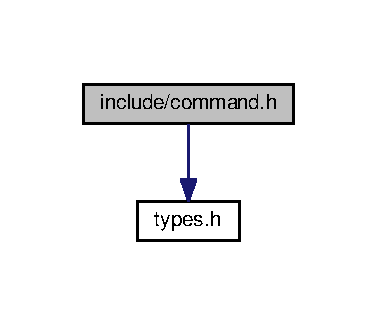
\includegraphics[width=181pt]{command_8h__incl}
\end{center}
\end{figure}
This graph shows which files directly or indirectly include this file\+:\nopagebreak
\begin{figure}[H]
\begin{center}
\leavevmode
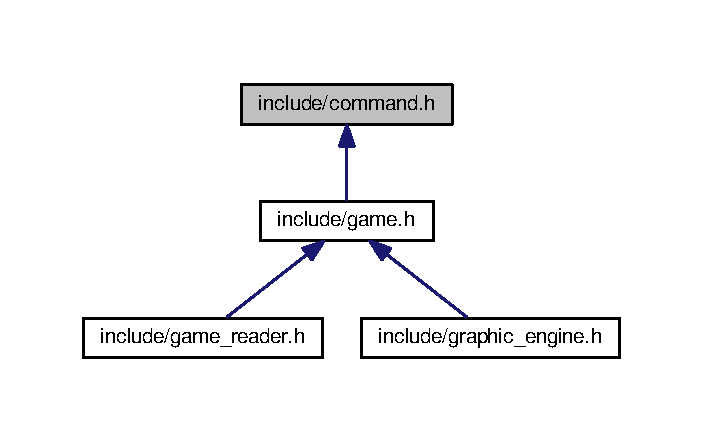
\includegraphics[width=338pt]{command_8h__dep__incl}
\end{center}
\end{figure}
\subsection*{Typedefs}
\begin{DoxyCompactItemize}
\item 
typedef struct \+\_\+\+Command \hyperlink{command_8h_a7d2935971c252377cb0fc1c8545dc2bc}{Command}\hypertarget{command_8h_a7d2935971c252377cb0fc1c8545dc2bc}{}\label{command_8h_a7d2935971c252377cb0fc1c8545dc2bc}

\begin{DoxyCompactList}\small\item\em It holds the necessary data to manage a command. \end{DoxyCompactList}\end{DoxyCompactItemize}
\subsection*{Functions}
\begin{Indent}{\bf command\+\_\+create}\par
{\em It allocates the memory for a Command structure.

\begin{DoxyAuthor}{Author}
Alejandro Pascual 
\end{DoxyAuthor}
\begin{DoxyVersion}{Version}
1.\+0 
\end{DoxyVersion}
\begin{DoxyDate}{Date}
16-\/03-\/2018 
\end{DoxyDate}
\begin{DoxyReturn}{Returns}
A Command$\ast$. 
\end{DoxyReturn}
}\begin{DoxyCompactItemize}
\item 
\hyperlink{command_8h_a7d2935971c252377cb0fc1c8545dc2bc}{Command} $\ast$ {\bfseries command\+\_\+create} ()\hypertarget{command_8h_a3e1d59fed8f0eb039c403543477d2ce0}{}\label{command_8h_a3e1d59fed8f0eb039c403543477d2ce0}

\end{DoxyCompactItemize}
\end{Indent}
\begin{Indent}{\bf command\+\_\+destroy}\par
{\em It frees the memory of the passed Command$\ast$.

\begin{DoxyAuthor}{Author}
Alejandro Pascual 
\end{DoxyAuthor}
\begin{DoxyVersion}{Version}
1.\+0 
\end{DoxyVersion}
\begin{DoxyDate}{Date}
16-\/03-\/2018 
\end{DoxyDate}

\begin{DoxyParams}{Parameters}
{\em Command$\ast$} & -\/$>$ The command to be freed.. \\
\hline
\end{DoxyParams}
\begin{DoxyReturn}{Returns}
A S\+T\+A\+T\+US, which indicates if the process was executed successfully or not. 
\end{DoxyReturn}
}\begin{DoxyCompactItemize}
\item 
\hyperlink{types_8h_a32c27cc471df37f4fc818d65de0a56c4}{S\+T\+A\+T\+US} {\bfseries command\+\_\+destroy} (\hyperlink{command_8h_a7d2935971c252377cb0fc1c8545dc2bc}{Command} $\ast$)\hypertarget{command_8h_ae919104b5b495669dd15a77936b1affe}{}\label{command_8h_ae919104b5b495669dd15a77936b1affe}

\end{DoxyCompactItemize}
\end{Indent}
\begin{Indent}{\bf command\+\_\+get\+\_\+user\+\_\+input}\par
{\em It gets an input command from the user.

\begin{DoxyAuthor}{Author}
Profesores P\+P\+R\+OG, edited by Victor Yrazusta and Alejandro Pascual 
\end{DoxyAuthor}
\begin{DoxyVersion}{Version}
3.\+0 
\end{DoxyVersion}
\begin{DoxyDate}{Date}
07-\/03-\/2018 
\end{DoxyDate}

\begin{DoxyParams}{Parameters}
{\em Command$\ast$} & -\/$>$ a command in which the input from the user will be stored. \\
\hline
\end{DoxyParams}
\begin{DoxyReturn}{Returns}
A S\+T\+A\+T\+US, which indicates if the process was executed successfully or not. 
\end{DoxyReturn}
}\begin{DoxyCompactItemize}
\item 
\hyperlink{types_8h_a32c27cc471df37f4fc818d65de0a56c4}{S\+T\+A\+T\+US} {\bfseries command\+\_\+get\+\_\+user\+\_\+input} (\hyperlink{command_8h_a7d2935971c252377cb0fc1c8545dc2bc}{Command} $\ast$)\hypertarget{command_8h_a1ceff4b9ade6a5381c217d28c80b1980}{}\label{command_8h_a1ceff4b9ade6a5381c217d28c80b1980}

\end{DoxyCompactItemize}
\end{Indent}
\begin{Indent}{\bf command\+\_\+get\+\_\+command}\par
{\em It returns the T\+\_\+\+Command of the Command$\ast$ passed as an argument.

\begin{DoxyAuthor}{Author}
Víctor Yrazusta 
\end{DoxyAuthor}
\begin{DoxyVersion}{Version}
1.\+0 
\end{DoxyVersion}
\begin{DoxyDate}{Date}
07-\/03-\/2018 
\end{DoxyDate}

\begin{DoxyParams}{Parameters}
{\em Command$\ast$} & -\/$>$ a command whose T\+\_\+\+Command will be returned. \\
\hline
\end{DoxyParams}
\begin{DoxyReturn}{Returns}
A T\+\_\+\+Command, which could be \char`\"{}\+N\+O\+\_\+\+C\+M\+D\char`\"{} if the passed pointer is N\+U\+LL, or the command\textquotesingle{}s T\+\_\+\+Command otherwise. 
\end{DoxyReturn}
}\begin{DoxyCompactItemize}
\item 
\hyperlink{types_8h_a92dd10a73cd77d692dff6c0b2af222f9}{T\+\_\+\+Command} {\bfseries command\+\_\+get\+\_\+command} (\hyperlink{command_8h_a7d2935971c252377cb0fc1c8545dc2bc}{Command} $\ast$)\hypertarget{command_8h_a699dacccff25074bc2ee5cde22dcebd8}{}\label{command_8h_a699dacccff25074bc2ee5cde22dcebd8}

\end{DoxyCompactItemize}
\end{Indent}
\begin{Indent}{\bf command\+\_\+get\+\_\+info}\par
{\em It returns the info of the Command$\ast$ passed as an argument.

\begin{DoxyAuthor}{Author}
Víctor Yrazusta 
\end{DoxyAuthor}
\begin{DoxyVersion}{Version}
1.\+0 
\end{DoxyVersion}
\begin{DoxyDate}{Date}
07-\/03-\/2018 
\end{DoxyDate}

\begin{DoxyParams}{Parameters}
{\em Command$\ast$} & -\/$>$ a command whose info will be returned. \\
\hline
\end{DoxyParams}
\begin{DoxyReturn}{Returns}
A char$\ast$, which could be N\+U\+LL if the passed pointer is N\+U\+LL, or the command\textquotesingle{}s info otherwise. 
\end{DoxyReturn}
}\begin{DoxyCompactItemize}
\item 
char $\ast$ {\bfseries command\+\_\+get\+\_\+info} (\hyperlink{command_8h_a7d2935971c252377cb0fc1c8545dc2bc}{Command} $\ast$)\hypertarget{command_8h_a449b3e73c4f9b35bec3de911d9092fe2}{}\label{command_8h_a449b3e73c4f9b35bec3de911d9092fe2}

\end{DoxyCompactItemize}
\end{Indent}
\begin{Indent}{\bf command\+\_\+print}\par
{\em It prints on the standard output the values of the command passed as an argument.

\begin{DoxyAuthor}{Author}
Víctor Yrazusta 
\end{DoxyAuthor}
\begin{DoxyVersion}{Version}
1.\+0 
\end{DoxyVersion}
\begin{DoxyDate}{Date}
07-\/03-\/2018 
\end{DoxyDate}

\begin{DoxyParams}{Parameters}
{\em Command$\ast$} & -\/$>$ a command whose data will be printed. \\
\hline
\end{DoxyParams}
\begin{DoxyReturn}{Returns}
An S\+T\+A\+T\+US, which could be \char`\"{}\+E\+R\+R\+O\+R\char`\"{} if the pointer passed as an argument is N\+U\+LL, or \char`\"{}\+O\+K\char`\"{} otherwise.
\end{DoxyReturn}
N\+O\+TE\+: This function was created for debugging purposes only and it is not used in the normal execution of the game. }\begin{DoxyCompactItemize}
\item 
\hyperlink{types_8h_a32c27cc471df37f4fc818d65de0a56c4}{S\+T\+A\+T\+US} {\bfseries command\+\_\+print} (\hyperlink{command_8h_a7d2935971c252377cb0fc1c8545dc2bc}{Command} $\ast$)\hypertarget{command_8h_ad528a0862548455323650212bfdb0c7a}{}\label{command_8h_ad528a0862548455323650212bfdb0c7a}

\end{DoxyCompactItemize}
\end{Indent}
\begin{Indent}{\bf command\+\_\+get\+\_\+str}\par
{\em This function gets the Command as a char to be used on the graphic\+\_\+engine.

\begin{DoxyAuthor}{Author}
Eric Morales edited by Victor Yrazusta 
\end{DoxyAuthor}
\begin{DoxyVersion}{Version}
2.\+0 
\end{DoxyVersion}
\begin{DoxyDate}{Date}
19-\/02-\/2018 
\end{DoxyDate}

\begin{DoxyParams}{Parameters}
{\em Command$\ast$} & -\/$>$ a command we will get the string from. \\
\hline
\end{DoxyParams}
\begin{DoxyReturn}{Returns}
A const char$\ast$ with the string of the command. 
\end{DoxyReturn}
}\begin{DoxyCompactItemize}
\item 
const char $\ast$ {\bfseries command\+\_\+get\+\_\+str} (\hyperlink{types_8h_a92dd10a73cd77d692dff6c0b2af222f9}{T\+\_\+\+Command})\hypertarget{command_8h_a3ed26a34c16490917ff3cc0e8c372667}{}\label{command_8h_a3ed26a34c16490917ff3cc0e8c372667}

\end{DoxyCompactItemize}
\end{Indent}


\subsection{Detailed Description}
It implements the command interpreter and the necessary functions to work with it. 

\begin{DoxyAuthor}{Author}
Profesores P\+P\+R\+OG edited by Victor Irazustra, Alejandro Pascual, Eric Morales. 
\end{DoxyAuthor}
\begin{DoxyVersion}{Version}
3.\+0 
\end{DoxyVersion}
\begin{DoxyDate}{Date}
19-\/12-\/2014 (creation) 02-\/04-\/2018 (last edit). 
\end{DoxyDate}
\begin{DoxyCopyright}{Copyright}
G\+NU Public License. 
\end{DoxyCopyright}

\hypertarget{command__test_8h}{}\section{include/command\+\_\+test.h File Reference}
\label{command__test_8h}\index{include/command\+\_\+test.\+h@{include/command\+\_\+test.\+h}}


It declares the tests for the command module.  


\subsection*{Functions}
\begin{DoxyCompactItemize}
\item 
void \hyperlink{command__test_8h_abed44af325fd42a3f4f4aa134315435c}{test1\+\_\+command\+\_\+create} ()
\item 
void \hyperlink{command__test_8h_aadf731a98e5122e70ede7cdc68ba621f}{test1\+\_\+command\+\_\+destroy} ()
\item 
void \hyperlink{command__test_8h_ad445f3e81035d4ab32ebc1526eb83fcb}{test2\+\_\+command\+\_\+destroy} ()
\item 
void \hyperlink{command__test_8h_a932afa8fb63c9b8ba551d030886ce491}{test1\+\_\+command\+\_\+get\+\_\+user\+\_\+input} ()
\item 
void \hyperlink{command__test_8h_a3ba7658db8aa069706b344d42ceabfaa}{test2\+\_\+command\+\_\+get\+\_\+user\+\_\+input} ()
\item 
void \hyperlink{command__test_8h_ae2d4b758fa9767317795c822b7334dec}{test3\+\_\+command\+\_\+get\+\_\+user\+\_\+input} ()
\item 
void \hyperlink{command__test_8h_aa5f2c4937af80de245778a8ac348cf3b}{test1\+\_\+command\+\_\+get\+\_\+command} ()
\item 
void \hyperlink{command__test_8h_a9c9d95687224d936e9486c0421969411}{test2\+\_\+command\+\_\+get\+\_\+command} ()
\item 
void \hyperlink{command__test_8h_a6aa58960e0653f7a4fb5c30350d64e54}{test1\+\_\+command\+\_\+get\+\_\+info} ()
\item 
void \hyperlink{command__test_8h_a057697416fb8f5d97d82f18b5f231930}{test2\+\_\+command\+\_\+get\+\_\+info} ()
\end{DoxyCompactItemize}


\subsection{Detailed Description}
It declares the tests for the command module. 

\begin{DoxyAuthor}{Author}
Victor Yrazusta 
\end{DoxyAuthor}
\begin{DoxyVersion}{Version}
1.\+0 
\end{DoxyVersion}
\begin{DoxyDate}{Date}
07-\/04-\/2018 (creation) 
\end{DoxyDate}
\begin{DoxyCopyright}{Copyright}
G\+NU Public License 
\end{DoxyCopyright}


\subsection{Function Documentation}
\index{command\+\_\+test.\+h@{command\+\_\+test.\+h}!test1\+\_\+command\+\_\+create@{test1\+\_\+command\+\_\+create}}
\index{test1\+\_\+command\+\_\+create@{test1\+\_\+command\+\_\+create}!command\+\_\+test.\+h@{command\+\_\+test.\+h}}
\subsubsection[{\texorpdfstring{test1\+\_\+command\+\_\+create()}{test1_command_create()}}]{\setlength{\rightskip}{0pt plus 5cm}void test1\+\_\+command\+\_\+create (
\begin{DoxyParamCaption}
{}
\end{DoxyParamCaption}
)}\hypertarget{command__test_8h_abed44af325fd42a3f4f4aa134315435c}{}\label{command__test_8h_abed44af325fd42a3f4f4aa134315435c}
\begin{DoxyRefDesc}{Test}
\item[\hyperlink{test__test000001}{Test}]Test command creation \end{DoxyRefDesc}
\begin{DoxyPrecond}{Precondition}
Nothing 
\end{DoxyPrecond}
\begin{DoxyPostcond}{Postcondition}
Non N\+U\+LL pointer to command 
\end{DoxyPostcond}
\index{command\+\_\+test.\+h@{command\+\_\+test.\+h}!test1\+\_\+command\+\_\+destroy@{test1\+\_\+command\+\_\+destroy}}
\index{test1\+\_\+command\+\_\+destroy@{test1\+\_\+command\+\_\+destroy}!command\+\_\+test.\+h@{command\+\_\+test.\+h}}
\subsubsection[{\texorpdfstring{test1\+\_\+command\+\_\+destroy()}{test1_command_destroy()}}]{\setlength{\rightskip}{0pt plus 5cm}void test1\+\_\+command\+\_\+destroy (
\begin{DoxyParamCaption}
{}
\end{DoxyParamCaption}
)}\hypertarget{command__test_8h_aadf731a98e5122e70ede7cdc68ba621f}{}\label{command__test_8h_aadf731a98e5122e70ede7cdc68ba621f}
\begin{DoxyRefDesc}{Test}
\item[\hyperlink{test__test000002}{Test}]Test command destruction \end{DoxyRefDesc}
\begin{DoxyPrecond}{Precondition}
A non N\+U\+LL pointer 
\end{DoxyPrecond}
\begin{DoxyPostcond}{Postcondition}
Output == OK 
\end{DoxyPostcond}
\index{command\+\_\+test.\+h@{command\+\_\+test.\+h}!test1\+\_\+command\+\_\+get\+\_\+command@{test1\+\_\+command\+\_\+get\+\_\+command}}
\index{test1\+\_\+command\+\_\+get\+\_\+command@{test1\+\_\+command\+\_\+get\+\_\+command}!command\+\_\+test.\+h@{command\+\_\+test.\+h}}
\subsubsection[{\texorpdfstring{test1\+\_\+command\+\_\+get\+\_\+command()}{test1_command_get_command()}}]{\setlength{\rightskip}{0pt plus 5cm}void test1\+\_\+command\+\_\+get\+\_\+command (
\begin{DoxyParamCaption}
{}
\end{DoxyParamCaption}
)}\hypertarget{command__test_8h_aa5f2c4937af80de245778a8ac348cf3b}{}\label{command__test_8h_aa5f2c4937af80de245778a8ac348cf3b}
\begin{DoxyRefDesc}{Test}
\item[\hyperlink{test__test000007}{Test}]Test command for reading command-\/$>$command setting \end{DoxyRefDesc}
\begin{DoxyPrecond}{Precondition}
A correct command and file 
\end{DoxyPrecond}
\begin{DoxyPostcond}{Postcondition}
Read command == Passed command 
\end{DoxyPostcond}
\index{command\+\_\+test.\+h@{command\+\_\+test.\+h}!test1\+\_\+command\+\_\+get\+\_\+info@{test1\+\_\+command\+\_\+get\+\_\+info}}
\index{test1\+\_\+command\+\_\+get\+\_\+info@{test1\+\_\+command\+\_\+get\+\_\+info}!command\+\_\+test.\+h@{command\+\_\+test.\+h}}
\subsubsection[{\texorpdfstring{test1\+\_\+command\+\_\+get\+\_\+info()}{test1_command_get_info()}}]{\setlength{\rightskip}{0pt plus 5cm}void test1\+\_\+command\+\_\+get\+\_\+info (
\begin{DoxyParamCaption}
{}
\end{DoxyParamCaption}
)}\hypertarget{command__test_8h_a6aa58960e0653f7a4fb5c30350d64e54}{}\label{command__test_8h_a6aa58960e0653f7a4fb5c30350d64e54}
\begin{DoxyRefDesc}{Test}
\item[\hyperlink{test__test000009}{Test}]Test command for reading command-\/$>$info setting \end{DoxyRefDesc}
\begin{DoxyPrecond}{Precondition}
A correct command and file 
\end{DoxyPrecond}
\begin{DoxyPostcond}{Postcondition}
Read info == Passed info 
\end{DoxyPostcond}
\index{command\+\_\+test.\+h@{command\+\_\+test.\+h}!test1\+\_\+command\+\_\+get\+\_\+user\+\_\+input@{test1\+\_\+command\+\_\+get\+\_\+user\+\_\+input}}
\index{test1\+\_\+command\+\_\+get\+\_\+user\+\_\+input@{test1\+\_\+command\+\_\+get\+\_\+user\+\_\+input}!command\+\_\+test.\+h@{command\+\_\+test.\+h}}
\subsubsection[{\texorpdfstring{test1\+\_\+command\+\_\+get\+\_\+user\+\_\+input()}{test1_command_get_user_input()}}]{\setlength{\rightskip}{0pt plus 5cm}void test1\+\_\+command\+\_\+get\+\_\+user\+\_\+input (
\begin{DoxyParamCaption}
{}
\end{DoxyParamCaption}
)}\hypertarget{command__test_8h_a932afa8fb63c9b8ba551d030886ce491}{}\label{command__test_8h_a932afa8fb63c9b8ba551d030886ce491}
\begin{DoxyRefDesc}{Test}
\item[\hyperlink{test__test000004}{Test}]Test command input \end{DoxyRefDesc}
\begin{DoxyPrecond}{Precondition}
A correct command pointer and file 
\end{DoxyPrecond}
\begin{DoxyPostcond}{Postcondition}
Output == OK 
\end{DoxyPostcond}
\index{command\+\_\+test.\+h@{command\+\_\+test.\+h}!test2\+\_\+command\+\_\+destroy@{test2\+\_\+command\+\_\+destroy}}
\index{test2\+\_\+command\+\_\+destroy@{test2\+\_\+command\+\_\+destroy}!command\+\_\+test.\+h@{command\+\_\+test.\+h}}
\subsubsection[{\texorpdfstring{test2\+\_\+command\+\_\+destroy()}{test2_command_destroy()}}]{\setlength{\rightskip}{0pt plus 5cm}void test2\+\_\+command\+\_\+destroy (
\begin{DoxyParamCaption}
{}
\end{DoxyParamCaption}
)}\hypertarget{command__test_8h_ad445f3e81035d4ab32ebc1526eb83fcb}{}\label{command__test_8h_ad445f3e81035d4ab32ebc1526eb83fcb}
\begin{DoxyRefDesc}{Test}
\item[\hyperlink{test__test000003}{Test}]Test command destruction \end{DoxyRefDesc}
\begin{DoxyPrecond}{Precondition}
A N\+U\+LL pointer 
\end{DoxyPrecond}
\begin{DoxyPostcond}{Postcondition}
Output == E\+R\+R\+OR 
\end{DoxyPostcond}
\index{command\+\_\+test.\+h@{command\+\_\+test.\+h}!test2\+\_\+command\+\_\+get\+\_\+command@{test2\+\_\+command\+\_\+get\+\_\+command}}
\index{test2\+\_\+command\+\_\+get\+\_\+command@{test2\+\_\+command\+\_\+get\+\_\+command}!command\+\_\+test.\+h@{command\+\_\+test.\+h}}
\subsubsection[{\texorpdfstring{test2\+\_\+command\+\_\+get\+\_\+command()}{test2_command_get_command()}}]{\setlength{\rightskip}{0pt plus 5cm}void test2\+\_\+command\+\_\+get\+\_\+command (
\begin{DoxyParamCaption}
{}
\end{DoxyParamCaption}
)}\hypertarget{command__test_8h_a9c9d95687224d936e9486c0421969411}{}\label{command__test_8h_a9c9d95687224d936e9486c0421969411}
\begin{DoxyRefDesc}{Test}
\item[\hyperlink{test__test000008}{Test}]Test command for reading command-\/$>$command setting \end{DoxyRefDesc}
\begin{DoxyPrecond}{Precondition}
A N\+U\+LL pointer to command 
\end{DoxyPrecond}
\begin{DoxyPostcond}{Postcondition}
Read command == N\+O\+\_\+\+C\+MD 
\end{DoxyPostcond}
\index{command\+\_\+test.\+h@{command\+\_\+test.\+h}!test2\+\_\+command\+\_\+get\+\_\+info@{test2\+\_\+command\+\_\+get\+\_\+info}}
\index{test2\+\_\+command\+\_\+get\+\_\+info@{test2\+\_\+command\+\_\+get\+\_\+info}!command\+\_\+test.\+h@{command\+\_\+test.\+h}}
\subsubsection[{\texorpdfstring{test2\+\_\+command\+\_\+get\+\_\+info()}{test2_command_get_info()}}]{\setlength{\rightskip}{0pt plus 5cm}void test2\+\_\+command\+\_\+get\+\_\+info (
\begin{DoxyParamCaption}
{}
\end{DoxyParamCaption}
)}\hypertarget{command__test_8h_a057697416fb8f5d97d82f18b5f231930}{}\label{command__test_8h_a057697416fb8f5d97d82f18b5f231930}
\begin{DoxyRefDesc}{Test}
\item[\hyperlink{test__test000010}{Test}]Test command for reading command-\/$>$info setting \end{DoxyRefDesc}
\begin{DoxyPrecond}{Precondition}
A N\+U\+LL pointer to command 
\end{DoxyPrecond}
\begin{DoxyPostcond}{Postcondition}
Read info == N\+U\+LL 
\end{DoxyPostcond}
\index{command\+\_\+test.\+h@{command\+\_\+test.\+h}!test2\+\_\+command\+\_\+get\+\_\+user\+\_\+input@{test2\+\_\+command\+\_\+get\+\_\+user\+\_\+input}}
\index{test2\+\_\+command\+\_\+get\+\_\+user\+\_\+input@{test2\+\_\+command\+\_\+get\+\_\+user\+\_\+input}!command\+\_\+test.\+h@{command\+\_\+test.\+h}}
\subsubsection[{\texorpdfstring{test2\+\_\+command\+\_\+get\+\_\+user\+\_\+input()}{test2_command_get_user_input()}}]{\setlength{\rightskip}{0pt plus 5cm}void test2\+\_\+command\+\_\+get\+\_\+user\+\_\+input (
\begin{DoxyParamCaption}
{}
\end{DoxyParamCaption}
)}\hypertarget{command__test_8h_a3ba7658db8aa069706b344d42ceabfaa}{}\label{command__test_8h_a3ba7658db8aa069706b344d42ceabfaa}
\begin{DoxyRefDesc}{Test}
\item[\hyperlink{test__test000005}{Test}]Test command input \end{DoxyRefDesc}
\begin{DoxyPrecond}{Precondition}
An incorrect command pointer but a correct file 
\end{DoxyPrecond}
\begin{DoxyPostcond}{Postcondition}
Output == E\+R\+R\+OR 
\end{DoxyPostcond}
\index{command\+\_\+test.\+h@{command\+\_\+test.\+h}!test3\+\_\+command\+\_\+get\+\_\+user\+\_\+input@{test3\+\_\+command\+\_\+get\+\_\+user\+\_\+input}}
\index{test3\+\_\+command\+\_\+get\+\_\+user\+\_\+input@{test3\+\_\+command\+\_\+get\+\_\+user\+\_\+input}!command\+\_\+test.\+h@{command\+\_\+test.\+h}}
\subsubsection[{\texorpdfstring{test3\+\_\+command\+\_\+get\+\_\+user\+\_\+input()}{test3_command_get_user_input()}}]{\setlength{\rightskip}{0pt plus 5cm}void test3\+\_\+command\+\_\+get\+\_\+user\+\_\+input (
\begin{DoxyParamCaption}
{}
\end{DoxyParamCaption}
)}\hypertarget{command__test_8h_ae2d4b758fa9767317795c822b7334dec}{}\label{command__test_8h_ae2d4b758fa9767317795c822b7334dec}
\begin{DoxyRefDesc}{Test}
\item[\hyperlink{test__test000006}{Test}]Test command input \end{DoxyRefDesc}
\begin{DoxyPrecond}{Precondition}
A correct command and file 
\end{DoxyPrecond}
\begin{DoxyPostcond}{Postcondition}
Registered command == Passed command 
\end{DoxyPostcond}

\hypertarget{die_8h}{}\section{include/die.h File Reference}
\label{die_8h}\index{include/die.\+h@{include/die.\+h}}


It defines a die and the different functions it needs to be managed.  


{\ttfamily \#include \char`\"{}types.\+h\char`\"{}}\\*
Include dependency graph for die.\+h\+:\nopagebreak
\begin{figure}[H]
\begin{center}
\leavevmode
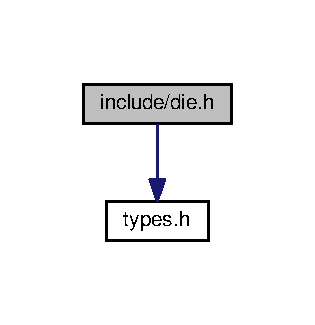
\includegraphics[width=151pt]{die_8h__incl}
\end{center}
\end{figure}
This graph shows which files directly or indirectly include this file\+:\nopagebreak
\begin{figure}[H]
\begin{center}
\leavevmode
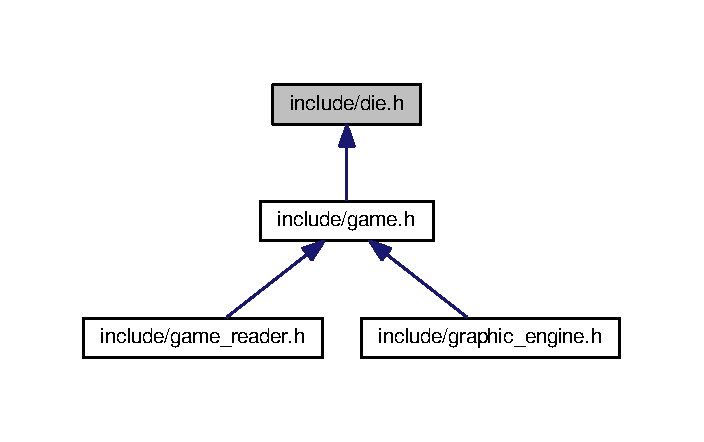
\includegraphics[width=338pt]{die_8h__dep__incl}
\end{center}
\end{figure}
\subsection*{Typedefs}
\begin{DoxyCompactItemize}
\item 
typedef struct \+\_\+\+Die \hyperlink{die_8h_a892f0b0bf81d69a1f7a14ea238e36dd3}{Die}\hypertarget{die_8h_a892f0b0bf81d69a1f7a14ea238e36dd3}{}\label{die_8h_a892f0b0bf81d69a1f7a14ea238e36dd3}

\begin{DoxyCompactList}\small\item\em It holds the necessary data to manage a die. \end{DoxyCompactList}\end{DoxyCompactItemize}
\subsection*{Functions}
\begin{Indent}{\bf die\+\_\+create}\par
{\em It creates a die with the id and number of faces passed.

\begin{DoxyAuthor}{Author}
Víctor Yrazusta 
\end{DoxyAuthor}
\begin{DoxyVersion}{Version}
1.\+0 
\end{DoxyVersion}
\begin{DoxyDate}{Date}
23-\/02-\/2018 
\end{DoxyDate}

\begin{DoxyParams}{Parameters}
{\em Id} & -\/$>$ an id which will be the Id of the die created. \\
\hline
{\em int} & -\/$>$ an integer, which will be the number of faces of the die created. \\
\hline
\end{DoxyParams}
\begin{DoxyReturn}{Returns}
A Die$\ast$, which points towards the created die. 
\end{DoxyReturn}
}\begin{DoxyCompactItemize}
\item 
\hyperlink{die_8h_a892f0b0bf81d69a1f7a14ea238e36dd3}{Die} $\ast$ {\bfseries die\+\_\+create} (\hyperlink{types_8h_a845e604fb28f7e3d97549da3448149d3}{Id}, int n\+Faces)\hypertarget{die_8h_a6860d03c4643311ec805a901a005ccc2}{}\label{die_8h_a6860d03c4643311ec805a901a005ccc2}

\end{DoxyCompactItemize}
\end{Indent}
\begin{Indent}{\bf die\+\_\+destroy}\par
{\em It deallocates the memory reserved for the Die$\ast$ passed.

\begin{DoxyAuthor}{Author}
Víctor Yrazusta 
\end{DoxyAuthor}
\begin{DoxyVersion}{Version}
1.\+0 
\end{DoxyVersion}
\begin{DoxyDate}{Date}
23-\/02-\/2018 
\end{DoxyDate}

\begin{DoxyParams}{Parameters}
{\em Die$\ast$} & -\/$>$ the die which will be deallocated. \\
\hline
\end{DoxyParams}
\begin{DoxyReturn}{Returns}
A S\+T\+A\+T\+US, which could be E\+R\+R\+OR if the pointer passed as an argument is N\+U\+LL, or OK otherwise. 
\end{DoxyReturn}
}\begin{DoxyCompactItemize}
\item 
\hyperlink{types_8h_a32c27cc471df37f4fc818d65de0a56c4}{S\+T\+A\+T\+US} {\bfseries die\+\_\+destroy} (\hyperlink{die_8h_a892f0b0bf81d69a1f7a14ea238e36dd3}{Die} $\ast$)\hypertarget{die_8h_a17ce6288dadfa1781013886e02568b25}{}\label{die_8h_a17ce6288dadfa1781013886e02568b25}

\end{DoxyCompactItemize}
\end{Indent}
\begin{Indent}{\bf die\+\_\+get\+\_\+id}\par
{\em It gets the Id of the given Die (as an argument).

\begin{DoxyAuthor}{Author}
Eric Morales 
\end{DoxyAuthor}
\begin{DoxyVersion}{Version}
1.\+0 
\end{DoxyVersion}
\begin{DoxyDate}{Date}
20-\/03-\/2018 
\end{DoxyDate}

\begin{DoxyParams}{Parameters}
{\em Die$\ast$} & -\/$>$ a die which we will get the Id from. \\
\hline
\end{DoxyParams}
\begin{DoxyReturn}{Returns}
An Id, with the given Dies Id. 
\end{DoxyReturn}
}\begin{DoxyCompactItemize}
\item 
\hyperlink{types_8h_a845e604fb28f7e3d97549da3448149d3}{Id} {\bfseries die\+\_\+get\+\_\+id} (\hyperlink{die_8h_a892f0b0bf81d69a1f7a14ea238e36dd3}{Die} $\ast$)\hypertarget{die_8h_a269937eb645d95cae2ae797b5bc35a4c}{}\label{die_8h_a269937eb645d95cae2ae797b5bc35a4c}

\end{DoxyCompactItemize}
\end{Indent}
\begin{Indent}{\bf die\+\_\+get\+\_\+value}\par
{\em It gets the value of the last roll from the given Die (as an argument).

\begin{DoxyAuthor}{Author}
Eric Morales 
\end{DoxyAuthor}
\begin{DoxyVersion}{Version}
1.\+0 
\end{DoxyVersion}
\begin{DoxyDate}{Date}
20-\/03-\/2018 
\end{DoxyDate}

\begin{DoxyParams}{Parameters}
{\em Die$\ast$} & -\/$>$ a die which will give us its last roll value. \\
\hline
\end{DoxyParams}
\begin{DoxyReturn}{Returns}
An integer, with the last value of the die (might be 0 if never rolled before). 
\end{DoxyReturn}
}\begin{DoxyCompactItemize}
\item 
int {\bfseries die\+\_\+get\+\_\+value} (\hyperlink{die_8h_a892f0b0bf81d69a1f7a14ea238e36dd3}{Die} $\ast$die)\hypertarget{die_8h_a2dbbc4fa2cb5dca61e2f86dbfc66ff4d}{}\label{die_8h_a2dbbc4fa2cb5dca61e2f86dbfc66ff4d}

\end{DoxyCompactItemize}
\end{Indent}
\begin{Indent}{\bf die\+\_\+roll}\par
{\em It rolls the die passed as an argument.

\begin{DoxyAuthor}{Author}
Víctor Yrazusta 
\end{DoxyAuthor}
\begin{DoxyVersion}{Version}
1.\+0 
\end{DoxyVersion}
\begin{DoxyDate}{Date}
23-\/02-\/2018 
\end{DoxyDate}

\begin{DoxyParams}{Parameters}
{\em Die$\ast$} & -\/$>$ a die which will be rolled. \\
\hline
\end{DoxyParams}
\begin{DoxyReturn}{Returns}
An integer, which could be \char`\"{}-\/1\char`\"{} if the pointer passed as an argument is N\+U\+LL or if it refers to a die that has no faces, or the result of rolling the die otherwise. 
\end{DoxyReturn}
}\begin{DoxyCompactItemize}
\item 
int {\bfseries die\+\_\+roll} (\hyperlink{die_8h_a892f0b0bf81d69a1f7a14ea238e36dd3}{Die} $\ast$)\hypertarget{die_8h_a2226474b382c96e64f1f7259aaa60c2f}{}\label{die_8h_a2226474b382c96e64f1f7259aaa60c2f}

\end{DoxyCompactItemize}
\end{Indent}
\begin{Indent}{\bf die\+\_\+set\+\_\+n\+Faces}\par
{\em It changes the number of faces of the die to a new value.

\begin{DoxyAuthor}{Author}
Víctor Yrazusta 
\end{DoxyAuthor}
\begin{DoxyVersion}{Version}
1.\+0 
\end{DoxyVersion}
\begin{DoxyDate}{Date}
23-\/02-\/2018 
\end{DoxyDate}

\begin{DoxyParams}{Parameters}
{\em Die$\ast$} & -\/$>$ a die whose number of faces will be changed. \\
\hline
{\em int} & -\/$>$ an integer which will indicate the new number of faces for the die. \\
\hline
\end{DoxyParams}
\begin{DoxyReturn}{Returns}
A S\+T\+A\+T\+US, which could be \char`\"{}\+E\+R\+R\+O\+R\char`\"{} if the pointer passed as an argument is N\+U\+LL, or \char`\"{}\+O\+K\char`\"{} otherwise. 
\end{DoxyReturn}
}\begin{DoxyCompactItemize}
\item 
\hyperlink{types_8h_a32c27cc471df37f4fc818d65de0a56c4}{S\+T\+A\+T\+US} {\bfseries die\+\_\+set\+\_\+n\+Faces} (\hyperlink{die_8h_a892f0b0bf81d69a1f7a14ea238e36dd3}{Die} $\ast$, int n\+Faces)\hypertarget{die_8h_a566e5f434af2060a814acd064458e7b1}{}\label{die_8h_a566e5f434af2060a814acd064458e7b1}

\end{DoxyCompactItemize}
\end{Indent}
\begin{Indent}{\bf die\+\_\+print}\par
{\em It prints on the standard output the values of the die passed as an argument.

\begin{DoxyAuthor}{Author}
Víctor Yrazusta 
\end{DoxyAuthor}
\begin{DoxyVersion}{Version}
1.\+0 
\end{DoxyVersion}
\begin{DoxyDate}{Date}
23-\/02-\/2018 
\end{DoxyDate}

\begin{DoxyParams}{Parameters}
{\em Die$\ast$} & -\/$>$ a die whose data will be printed. \\
\hline
\end{DoxyParams}
\begin{DoxyReturn}{Returns}
A S\+T\+A\+T\+US, which could be \char`\"{}\+E\+R\+R\+O\+R\char`\"{} if the pointer passed as an argument is N\+U\+LL, or \char`\"{}\+O\+K\char`\"{} otherwise.
\end{DoxyReturn}
N\+O\+TE\+: This function was created for debugging purposes only and it is not used in the normal execution of the game. }\begin{DoxyCompactItemize}
\item 
\hyperlink{types_8h_a32c27cc471df37f4fc818d65de0a56c4}{S\+T\+A\+T\+US} {\bfseries die\+\_\+print} (\hyperlink{die_8h_a892f0b0bf81d69a1f7a14ea238e36dd3}{Die} $\ast$)\hypertarget{die_8h_aee81689a57f33a70edf28509f41df8a5}{}\label{die_8h_aee81689a57f33a70edf28509f41df8a5}

\end{DoxyCompactItemize}
\end{Indent}


\subsection{Detailed Description}
It defines a die and the different functions it needs to be managed. 

\begin{DoxyAuthor}{Author}
Víctor Yrazusta 
\end{DoxyAuthor}
\begin{DoxyVersion}{Version}
2.\+0 
\end{DoxyVersion}
\begin{DoxyDate}{Date}
13-\/02-\/2018 (creation) 22-\/03-\/2018 (last edit) 
\end{DoxyDate}
\begin{DoxyCopyright}{Copyright}
G\+NU Public License 
\end{DoxyCopyright}

\hypertarget{game_8h}{}\section{include/game.h File Reference}
\label{game_8h}\index{include/game.\+h@{include/game.\+h}}


It defines the game interface for each command and rest of needed functions.  


{\ttfamily \#include $<$stdlib.\+h$>$}\\*
{\ttfamily \#include \char`\"{}command.\+h\char`\"{}}\\*
{\ttfamily \#include \char`\"{}space.\+h\char`\"{}}\\*
{\ttfamily \#include \char`\"{}player.\+h\char`\"{}}\\*
{\ttfamily \#include \char`\"{}object.\+h\char`\"{}}\\*
{\ttfamily \#include \char`\"{}die.\+h\char`\"{}}\\*
{\ttfamily \#include \char`\"{}link.\+h\char`\"{}}\\*
Include dependency graph for game.\+h\+:\nopagebreak
\begin{figure}[H]
\begin{center}
\leavevmode
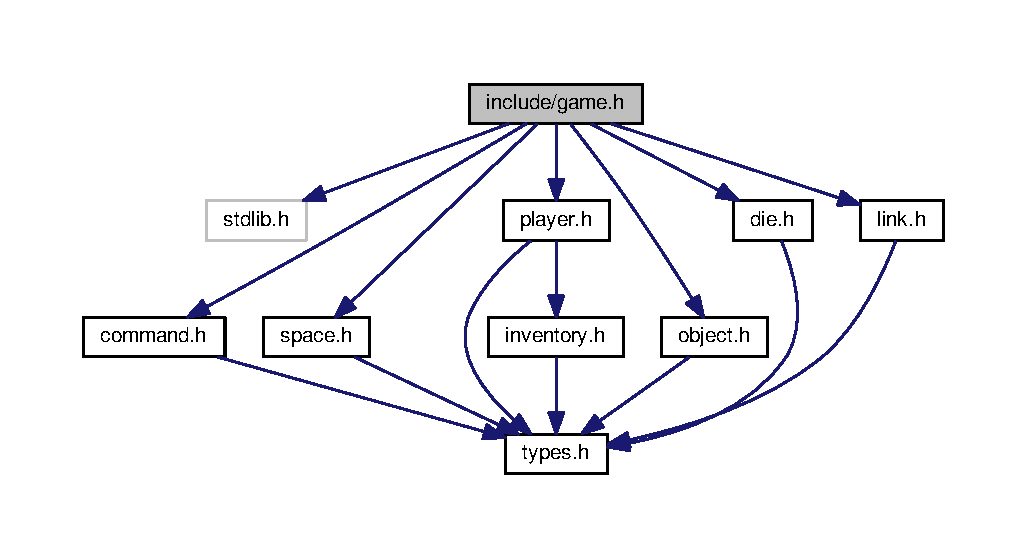
\includegraphics[width=350pt]{game_8h__incl}
\end{center}
\end{figure}
This graph shows which files directly or indirectly include this file\+:\nopagebreak
\begin{figure}[H]
\begin{center}
\leavevmode
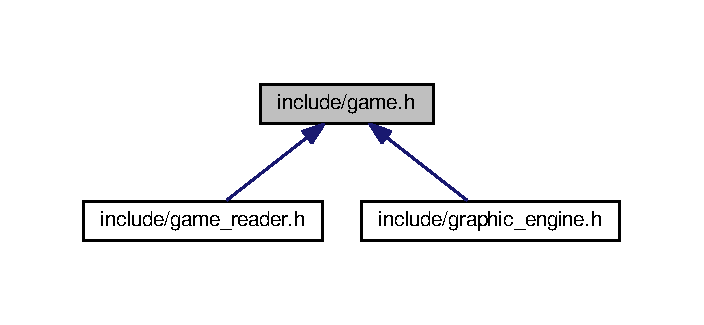
\includegraphics[width=338pt]{game_8h__dep__incl}
\end{center}
\end{figure}
\subsection*{Typedefs}
\begin{DoxyCompactItemize}
\item 
typedef struct \+\_\+\+Game \hyperlink{game_8h_a57156d39c530aec3fba3a9dad8c2dc6a}{Game}\hypertarget{game_8h_a57156d39c530aec3fba3a9dad8c2dc6a}{}\label{game_8h_a57156d39c530aec3fba3a9dad8c2dc6a}

\begin{DoxyCompactList}\small\item\em It holds the necessary data to manage a game. \end{DoxyCompactList}\end{DoxyCompactItemize}
\subsection*{Functions}
\begin{Indent}{\bf game\+\_\+create}\par
{\em It allocates memory for a game.

\begin{DoxyAuthor}{Author}
Victor Yrazusta edited by Eric Morales 
\end{DoxyAuthor}
\begin{DoxyVersion}{Version}
2.\+0 
\end{DoxyVersion}
\begin{DoxyDate}{Date}
27-\/02-\/2018 
\end{DoxyDate}
\begin{DoxyReturn}{Returns}
A game$\ast$, which could be N\+U\+LL if the function failed. 
\end{DoxyReturn}
}\begin{DoxyCompactItemize}
\item 
\hyperlink{game_8h_a57156d39c530aec3fba3a9dad8c2dc6a}{Game} $\ast$ {\bfseries game\+\_\+create} ()\hypertarget{game_8h_a1cdbe3f06b9bf49eb5e334a22ad3b2b9}{}\label{game_8h_a1cdbe3f06b9bf49eb5e334a22ad3b2b9}

\end{DoxyCompactItemize}
\end{Indent}
\begin{Indent}{\bf game\+\_\+create\+\_\+from\+\_\+file}\par
{\em It loads into a game (with already allocated memory) the data inside a file.

\begin{DoxyAuthor}{Author}
Victor Yrazusta edited by Eric Morales 
\end{DoxyAuthor}
\begin{DoxyVersion}{Version}
3.\+0 
\end{DoxyVersion}
\begin{DoxyDate}{Date}
27-\/02-\/2018 
\end{DoxyDate}

\begin{DoxyParams}{Parameters}
{\em Game$\ast$} & -\/$>$ a game in which the function will store the obtained data, creating all the needed things on it. \\
\hline
{\em char$\ast$} & -\/$>$ a string which will be the file (allready opened) that contains the information of the game. \\
\hline
\end{DoxyParams}
\begin{DoxyReturn}{Returns}
A S\+T\+A\+T\+US, which will tell if the function failed. 
\end{DoxyReturn}
}\begin{DoxyCompactItemize}
\item 
\hyperlink{types_8h_a32c27cc471df37f4fc818d65de0a56c4}{S\+T\+A\+T\+US} {\bfseries game\+\_\+create\+\_\+from\+\_\+file} (\hyperlink{game_8h_a57156d39c530aec3fba3a9dad8c2dc6a}{Game} $\ast$, char $\ast$file\+\_\+name)\hypertarget{game_8h_a4061ad53c9235ace67a6bc4cc95fe45d}{}\label{game_8h_a4061ad53c9235ace67a6bc4cc95fe45d}

\end{DoxyCompactItemize}
\end{Indent}
\begin{Indent}{\bf game\+\_\+update}\par
{\em It updates the game to the last command that was input.

\begin{DoxyAuthor}{Author}
Victor Yrazusta edited by Eric Morales 
\end{DoxyAuthor}
\begin{DoxyVersion}{Version}
3.\+0 
\end{DoxyVersion}
\begin{DoxyDate}{Date}
27-\/02-\/2018 
\end{DoxyDate}

\begin{DoxyParams}{Parameters}
{\em Game$\ast$} & -\/$>$ a game which will be updated depending on the last introduced command. \\
\hline
{\em Command$\ast$} & -\/$>$ a command which will be the last given command from the user. \\
\hline
\end{DoxyParams}
\begin{DoxyReturn}{Returns}
A S\+T\+A\+T\+US, which will tell if the function failed. 
\end{DoxyReturn}
}\begin{DoxyCompactItemize}
\item 
\hyperlink{types_8h_a32c27cc471df37f4fc818d65de0a56c4}{S\+T\+A\+T\+US} {\bfseries game\+\_\+update} (\hyperlink{game_8h_a57156d39c530aec3fba3a9dad8c2dc6a}{Game} $\ast$, \hyperlink{command_8h_a7d2935971c252377cb0fc1c8545dc2bc}{Command} $\ast$)\hypertarget{game_8h_a4ec0eb4cc473661ae1e3d049e7628b9f}{}\label{game_8h_a4ec0eb4cc473661ae1e3d049e7628b9f}

\end{DoxyCompactItemize}
\end{Indent}
\begin{Indent}{\bf game\+\_\+destroy}\par
{\em It finds an object, a player, a die or a space in the passed game$\ast$ whose Id is passed as an argument.

\begin{DoxyAuthor}{Author}
Victor Yrazusta edited by Eric Morales 
\end{DoxyAuthor}
\begin{DoxyVersion}{Version}
2.\+0 
\end{DoxyVersion}
\begin{DoxyDate}{Date}
27-\/02-\/2018 
\end{DoxyDate}

\begin{DoxyParams}{Parameters}
{\em Game$\ast$} & -\/$>$ a game in which the function will search for the Id. \\
\hline
{\em Id} & -\/$>$ an id which will be the Id of the struct found (if any). \\
\hline
\end{DoxyParams}
\begin{DoxyReturn}{Returns}
A S\+T\+A\+T\+US, which will tell if the function failed. 
\end{DoxyReturn}
}\begin{DoxyCompactItemize}
\item 
\hyperlink{types_8h_a32c27cc471df37f4fc818d65de0a56c4}{S\+T\+A\+T\+US} {\bfseries game\+\_\+destroy} (\hyperlink{game_8h_a57156d39c530aec3fba3a9dad8c2dc6a}{Game} $\ast$)\hypertarget{game_8h_accc8491f1e1f5cd64399fdde0058d5b2}{}\label{game_8h_accc8491f1e1f5cd64399fdde0058d5b2}

\end{DoxyCompactItemize}
\end{Indent}
\begin{Indent}{\bf game\+\_\+is over}\par
{\em It checks if the game is over or not (right now there are no conditions yet).

\begin{DoxyAuthor}{Author}
Profesores P\+P\+R\+OG 
\end{DoxyAuthor}
\begin{DoxyVersion}{Version}
1.\+0 
\end{DoxyVersion}
\begin{DoxyDate}{Date}
13-\/01-\/2015 
\end{DoxyDate}

\begin{DoxyParams}{Parameters}
{\em Game$\ast$} & -\/$>$ the game which we will check if its over or not. \\
\hline
\end{DoxyParams}
\begin{DoxyReturn}{Returns}
A B\+O\+OL telling if its ended or not. 
\end{DoxyReturn}
}\begin{DoxyCompactItemize}
\item 
\hyperlink{types_8h_a3e5b8192e7d9ffaf3542f1210aec18dd}{B\+O\+OL} {\bfseries game\+\_\+is\+\_\+over} (\hyperlink{game_8h_a57156d39c530aec3fba3a9dad8c2dc6a}{Game} $\ast$)\hypertarget{game_8h_a48225cf8a94551e4748e50d76e7017c3}{}\label{game_8h_a48225cf8a94551e4748e50d76e7017c3}

\end{DoxyCompactItemize}
\end{Indent}
\begin{Indent}{\bf game\+\_\+print\+\_\+data}\par
{\em It prints all the game data, for debugging purposes.

\begin{DoxyAuthor}{Author}
Profesores P\+P\+R\+OG edited by Victor Yrazusta 
\end{DoxyAuthor}
\begin{DoxyVersion}{Version}
2.\+0 
\end{DoxyVersion}
\begin{DoxyDate}{Date}
13-\/01-\/2015 (Creation) 07-\/04-\/2018 (Edited) 
\end{DoxyDate}

\begin{DoxyParams}{Parameters}
{\em Game$\ast$} & -\/$>$ which information will be printed (not graphic engine). \\
\hline
\end{DoxyParams}
\begin{DoxyReturn}{Returns}
A void without any relevant information. 
\end{DoxyReturn}
}\begin{DoxyCompactItemize}
\item 
void {\bfseries game\+\_\+print\+\_\+data} (\hyperlink{game_8h_a57156d39c530aec3fba3a9dad8c2dc6a}{Game} $\ast$)\hypertarget{game_8h_ad379d0f940eb8020d7fbc6d805c307f9}{}\label{game_8h_ad379d0f940eb8020d7fbc6d805c307f9}

\end{DoxyCompactItemize}
\end{Indent}
\begin{Indent}{\bf game\+\_\+add\+\_\+space}\par
{\em It adds a new space to the game.

\begin{DoxyAuthor}{Author}
Profesores P\+P\+R\+OG edited by Javier Lougedo 
\end{DoxyAuthor}
\begin{DoxyVersion}{Version}
1.\+0 
\end{DoxyVersion}
\begin{DoxyDate}{Date}
13-\/01-\/2015 
\end{DoxyDate}

\begin{DoxyParams}{Parameters}
{\em Game$\ast$} & -\/$>$ a game where the space will be added. \\
\hline
{\em Space$\ast$} & -\/$>$ carrying the space to be loaded. \\
\hline
\end{DoxyParams}
\begin{DoxyReturn}{Returns}
A S\+T\+A\+T\+US, which will tell if the function failed. 
\end{DoxyReturn}
}\begin{DoxyCompactItemize}
\item 
\hyperlink{types_8h_a32c27cc471df37f4fc818d65de0a56c4}{S\+T\+A\+T\+US} {\bfseries game\+\_\+add\+\_\+space} (\hyperlink{game_8h_a57156d39c530aec3fba3a9dad8c2dc6a}{Game} $\ast$, \hyperlink{space_8h_a67533ffc2b70463baecc38fb0629bbfc}{Space} $\ast$)\hypertarget{game_8h_a90f0011dd654de9aaef8f42db4d66294}{}\label{game_8h_a90f0011dd654de9aaef8f42db4d66294}

\end{DoxyCompactItemize}
\end{Indent}
\begin{Indent}{\bf game\+\_\+add\+\_\+object}\par
{\em It adds a new object to the game.

\begin{DoxyAuthor}{Author}
Alejandro Pascual edited by Javier Lougedo 
\end{DoxyAuthor}
\begin{DoxyVersion}{Version}
1.\+0 
\end{DoxyVersion}
\begin{DoxyDate}{Date}
11-\/03-\/2018 
\end{DoxyDate}

\begin{DoxyParams}{Parameters}
{\em Game$\ast$} & -\/$>$ a game where the object will be added. \\
\hline
{\em Object$\ast$} & -\/$>$ carrying the object to be loaded. \\
\hline
\end{DoxyParams}
\begin{DoxyReturn}{Returns}
A S\+T\+A\+T\+US, which will tell if the function failed. 
\end{DoxyReturn}
}\begin{DoxyCompactItemize}
\item 
\hyperlink{types_8h_a32c27cc471df37f4fc818d65de0a56c4}{S\+T\+A\+T\+US} {\bfseries game\+\_\+add\+\_\+object} (\hyperlink{game_8h_a57156d39c530aec3fba3a9dad8c2dc6a}{Game} $\ast$, \hyperlink{object_8h_a7f8bbcda919b65ce67f92fba08e0212f}{Object} $\ast$, \hyperlink{types_8h_a845e604fb28f7e3d97549da3448149d3}{Id} location\+\_\+id)\hypertarget{game_8h_a9adce4004adbbd7fd1c070ccef95921c}{}\label{game_8h_a9adce4004adbbd7fd1c070ccef95921c}

\end{DoxyCompactItemize}
\end{Indent}
\begin{Indent}{\bf game\+\_\+get\+\_\+spaces\+\_\+number}\par
{\em It returns the number of spaces there are in the game.

\begin{DoxyAuthor}{Author}
Victor Yrazusta 
\end{DoxyAuthor}
\begin{DoxyVersion}{Version}
1.\+0 
\end{DoxyVersion}
\begin{DoxyDate}{Date}
16-\/03-\/2018 
\end{DoxyDate}

\begin{DoxyParams}{Parameters}
{\em Game$\ast$} & -\/$>$ a game to check for the number of spaces in it. \\
\hline
\end{DoxyParams}
\begin{DoxyReturn}{Returns}
An int with the number of spaces. 
\end{DoxyReturn}
}\begin{DoxyCompactItemize}
\item 
int {\bfseries game\+\_\+get\+\_\+spaces\+\_\+number} (\hyperlink{game_8h_a57156d39c530aec3fba3a9dad8c2dc6a}{Game} $\ast$)\hypertarget{game_8h_a176cb01b6aacab9b7cdcea4fa46d2967}{}\label{game_8h_a176cb01b6aacab9b7cdcea4fa46d2967}

\end{DoxyCompactItemize}
\end{Indent}
\begin{Indent}{\bf game\+\_\+get\+\_\+players\+\_\+number}\par
{\em It returns the number of players there are in the game.

\begin{DoxyAuthor}{Author}
Alejandro Pascual 
\end{DoxyAuthor}
\begin{DoxyVersion}{Version}
1.\+0 
\end{DoxyVersion}
\begin{DoxyDate}{Date}
16-\/03-\/2018 
\end{DoxyDate}

\begin{DoxyParams}{Parameters}
{\em Game$\ast$} & -\/$>$ a game to check for the number of players in it. \\
\hline
\end{DoxyParams}
\begin{DoxyReturn}{Returns}
An int with the number of players. 
\end{DoxyReturn}
}\begin{DoxyCompactItemize}
\item 
int {\bfseries game\+\_\+get\+\_\+players\+\_\+number} (\hyperlink{game_8h_a57156d39c530aec3fba3a9dad8c2dc6a}{Game} $\ast$)\hypertarget{game_8h_a1746123c2f85e94cfc345dfeed67e3d5}{}\label{game_8h_a1746123c2f85e94cfc345dfeed67e3d5}

\end{DoxyCompactItemize}
\end{Indent}
\begin{Indent}{\bf game\+\_\+get\+\_\+objects\+\_\+number}\par
{\em It returns the number of objects there are in the game.

\begin{DoxyAuthor}{Author}
Victor Yrazusta 
\end{DoxyAuthor}
\begin{DoxyVersion}{Version}
1.\+0 
\end{DoxyVersion}
\begin{DoxyDate}{Date}
16-\/03-\/2018 
\end{DoxyDate}

\begin{DoxyParams}{Parameters}
{\em Game$\ast$} & -\/$>$ a game to check for the number of objects in it. \\
\hline
\end{DoxyParams}
\begin{DoxyReturn}{Returns}
An int with the number of objects. 
\end{DoxyReturn}
}\begin{DoxyCompactItemize}
\item 
int {\bfseries game\+\_\+get\+\_\+objects\+\_\+number} (\hyperlink{game_8h_a57156d39c530aec3fba3a9dad8c2dc6a}{Game} $\ast$)\hypertarget{game_8h_a696aed082f87baa862e422d48d44321c}{}\label{game_8h_a696aed082f87baa862e422d48d44321c}

\end{DoxyCompactItemize}
\end{Indent}
\begin{Indent}{\bf game\+\_\+get\+\_\+dies\+\_\+number}\par
{\em It returns the number of dies there are in the game.

\begin{DoxyAuthor}{Author}
Alejandro Pascual 
\end{DoxyAuthor}
\begin{DoxyVersion}{Version}
1.\+0 
\end{DoxyVersion}
\begin{DoxyDate}{Date}
16-\/03-\/2018 
\end{DoxyDate}

\begin{DoxyParams}{Parameters}
{\em Game$\ast$} & -\/$>$ a game to check for the number of dies in it. \\
\hline
\end{DoxyParams}
\begin{DoxyReturn}{Returns}
An int with the number of dies. 
\end{DoxyReturn}
}\begin{DoxyCompactItemize}
\item 
int {\bfseries game\+\_\+get\+\_\+dies\+\_\+number} (\hyperlink{game_8h_a57156d39c530aec3fba3a9dad8c2dc6a}{Game} $\ast$)\hypertarget{game_8h_afe2a116d3db04b2f7b074165a77ce10a}{}\label{game_8h_afe2a116d3db04b2f7b074165a77ce10a}

\end{DoxyCompactItemize}
\end{Indent}
\begin{Indent}{\bf game\+\_\+find}\par
{\em It finds an object, a player, a die or a space in the passed game$\ast$ whose Id is passed as an argument.

\begin{DoxyAuthor}{Author}
Victor Yrazusta 
\end{DoxyAuthor}
\begin{DoxyVersion}{Version}
2.\+0 
\end{DoxyVersion}
\begin{DoxyDate}{Date}
27-\/02-\/2018 
\end{DoxyDate}

\begin{DoxyParams}{Parameters}
{\em Game$\ast$} & -\/$>$ a game in which the function will search for the Id. \\
\hline
{\em Id} & -\/$>$ an id which will be the Id of the struct found (if any). \\
\hline
\end{DoxyParams}
\begin{DoxyReturn}{Returns}
A void$\ast$, which could be N\+U\+LL if the function fails to find an object, a player, a die or a space with the specified Id, or the object, player, die or space found otherwise. 
\end{DoxyReturn}
}\begin{DoxyCompactItemize}
\item 
void $\ast$ {\bfseries game\+\_\+find} (\hyperlink{game_8h_a57156d39c530aec3fba3a9dad8c2dc6a}{Game} $\ast$, \hyperlink{types_8h_a845e604fb28f7e3d97549da3448149d3}{Id} id)\hypertarget{game_8h_a3145940f5ae2b5d82a6271c062cc34a9}{}\label{game_8h_a3145940f5ae2b5d82a6271c062cc34a9}

\end{DoxyCompactItemize}
\end{Indent}
\begin{Indent}{\bf game\+\_\+find\+\_\+name}\par
{\em It finds an object, a player, a die or a space in the passed game$\ast$ whose name is passed as an argument.

\begin{DoxyAuthor}{Author}
Victor Yrazusta 
\end{DoxyAuthor}
\begin{DoxyVersion}{Version}
1.\+0 
\end{DoxyVersion}
\begin{DoxyDate}{Date}
28-\/02-\/2018 
\end{DoxyDate}

\begin{DoxyParams}{Parameters}
{\em Game$\ast$} & -\/$>$ a game in which the function will search for the name. \\
\hline
{\em char$\ast$} & -\/$>$ a string which will be the name of the struct found (if any). \\
\hline
\end{DoxyParams}
\begin{DoxyReturn}{Returns}
A void$\ast$, which could be N\+U\+LL if the function fails to find an object, a player, a die or a space with the specified Id, or the object, player, die or space found otherwise. 
\end{DoxyReturn}
}\begin{DoxyCompactItemize}
\item 
void $\ast$ {\bfseries game\+\_\+find\+\_\+name} (\hyperlink{game_8h_a57156d39c530aec3fba3a9dad8c2dc6a}{Game} $\ast$, char $\ast$name)\hypertarget{game_8h_a0410538a05363d74245854b77880ba44}{}\label{game_8h_a0410538a05363d74245854b77880ba44}

\end{DoxyCompactItemize}
\end{Indent}
\begin{Indent}{\bf game\+\_\+set\+\_\+object\+\_\+location}\par
{\em It changes the location of the passed object and the location id passed to register the new position of the object.

\begin{DoxyAuthor}{Author}
Victor Yrazusta 
\end{DoxyAuthor}
\begin{DoxyVersion}{Version}
1.\+0 
\end{DoxyVersion}
\begin{DoxyDate}{Date}
28-\/02-\/2018 
\end{DoxyDate}

\begin{DoxyParams}{Parameters}
{\em Game$\ast$} & -\/$>$ a game in which the function will search for the name. \\
\hline
{\em Id} & -\/$>$ the id of the location which will start holding the passed object Id. \\
\hline
{\em Id} & -\/$>$ an id with the Id of the object which will be registered by the locations. \\
\hline
\end{DoxyParams}
\begin{DoxyReturn}{Returns}
A S\+T\+A\+T\+US, which indicates if the process was executed successfully or not. 
\end{DoxyReturn}
}\begin{DoxyCompactItemize}
\item 
\hyperlink{types_8h_a32c27cc471df37f4fc818d65de0a56c4}{S\+T\+A\+T\+US} {\bfseries game\+\_\+set\+\_\+object\+\_\+location} (\hyperlink{game_8h_a57156d39c530aec3fba3a9dad8c2dc6a}{Game} $\ast$game, \hyperlink{types_8h_a845e604fb28f7e3d97549da3448149d3}{Id} location\+\_\+id, \hyperlink{types_8h_a845e604fb28f7e3d97549da3448149d3}{Id} object\+\_\+id)\hypertarget{game_8h_a1667ce6e1db1af644d89c96f18c4c674}{}\label{game_8h_a1667ce6e1db1af644d89c96f18c4c674}

\end{DoxyCompactItemize}
\end{Indent}
\begin{Indent}{\bf game\+\_\+get\+\_\+last\+\_\+command}\par
{\em It gets the last command that the user input, to print it.

\begin{DoxyAuthor}{Author}
Profesores P\+P\+R\+OG 
\end{DoxyAuthor}
\begin{DoxyVersion}{Version}
1.\+0 
\end{DoxyVersion}
\begin{DoxyDate}{Date}
13-\/01-\/2015 
\end{DoxyDate}

\begin{DoxyParams}{Parameters}
{\em Game$\ast$} & -\/$>$ a game where we will get the command from. \\
\hline
\end{DoxyParams}
\begin{DoxyReturn}{Returns}
A T\+\_\+\+Command (text) with the actual command. 
\end{DoxyReturn}
}\begin{DoxyCompactItemize}
\item 
\hyperlink{types_8h_a92dd10a73cd77d692dff6c0b2af222f9}{T\+\_\+\+Command} {\bfseries game\+\_\+get\+\_\+last\+\_\+command} (\hyperlink{game_8h_a57156d39c530aec3fba3a9dad8c2dc6a}{Game} $\ast$)\hypertarget{game_8h_a6fc72cfae5f97e7e3198ebba0feb45b3}{}\label{game_8h_a6fc72cfae5f97e7e3198ebba0feb45b3}

\end{DoxyCompactItemize}
\end{Indent}
\begin{Indent}{\bf game\+\_\+get\+\_\+status\+\_\+last\+\_\+command}\par
{\em It give us the status of the last command printed on the screen

\begin{DoxyAuthor}{Author}
Eric Morales 
\end{DoxyAuthor}
\begin{DoxyVersion}{Version}
1.\+0 
\end{DoxyVersion}
\begin{DoxyDate}{Date}
26-\/03-\/2018 
\end{DoxyDate}

\begin{DoxyParams}{Parameters}
{\em Game$\ast$} & -\/$>$ a game to get the last command status from. \\
\hline
\end{DoxyParams}
\begin{DoxyReturn}{Returns}
A S\+T\+A\+T\+US, the status of the command. 
\end{DoxyReturn}
}\begin{DoxyCompactItemize}
\item 
\hyperlink{types_8h_a32c27cc471df37f4fc818d65de0a56c4}{S\+T\+A\+T\+US} {\bfseries game\+\_\+get\+\_\+status\+\_\+last\+\_\+command} (\hyperlink{game_8h_a57156d39c530aec3fba3a9dad8c2dc6a}{Game} $\ast$game)\hypertarget{game_8h_aa864653e168ad9407ff4c9a7b3d6f436}{}\label{game_8h_aa864653e168ad9407ff4c9a7b3d6f436}

\end{DoxyCompactItemize}
\end{Indent}
\begin{Indent}{\bf game\+\_\+get\+\_\+last\+\_\+check}\par
{\em It gives us the last description ordered by the user.

\begin{DoxyAuthor}{Author}
Eric Morales 
\end{DoxyAuthor}
\begin{DoxyVersion}{Version}
1.\+0 
\end{DoxyVersion}
\begin{DoxyDate}{Date}
26-\/03-\/2018 
\end{DoxyDate}

\begin{DoxyParams}{Parameters}
{\em Game$\ast$} & -\/$>$ a game which will give us the description we are asking for. \\
\hline
\end{DoxyParams}
\begin{DoxyReturn}{Returns}
A const char$\ast$ with the description. 
\end{DoxyReturn}
}\begin{DoxyCompactItemize}
\item 
char $\ast$$\ast$ {\bfseries game\+\_\+get\+\_\+last\+\_\+check} (\hyperlink{game_8h_a57156d39c530aec3fba3a9dad8c2dc6a}{Game} $\ast$game)\hypertarget{game_8h_aa220681feb41d34cc4a5209af820102d}{}\label{game_8h_aa220681feb41d34cc4a5209af820102d}

\end{DoxyCompactItemize}
\end{Indent}
\begin{Indent}{\bf game\+\_\+add\+\_\+link}\par
{\em It adds a link to the game.

\begin{DoxyAuthor}{Author}
Eric Morales edited by Javier Lougedo 
\end{DoxyAuthor}
\begin{DoxyVersion}{Version}
1.\+0 
\end{DoxyVersion}
\begin{DoxyDate}{Date}
26-\/03-\/2018 
\end{DoxyDate}

\begin{DoxyParams}{Parameters}
{\em Game$\ast$} & -\/$>$ a game where we are playing. \\
\hline
{\em Link} & -\/$>$ a link with the added link. \\
\hline
\end{DoxyParams}
\begin{DoxyReturn}{Returns}
A S\+T\+A\+T\+US, OK if we can add the link or E\+R\+R\+OR if we have problems. 
\end{DoxyReturn}
}\begin{DoxyCompactItemize}
\item 
\hyperlink{types_8h_a32c27cc471df37f4fc818d65de0a56c4}{S\+T\+A\+T\+US} {\bfseries game\+\_\+add\+\_\+link} (\hyperlink{game_8h_a57156d39c530aec3fba3a9dad8c2dc6a}{Game} $\ast$game, \hyperlink{link_8h_ae3b299941e67be6971bfd64a25505eff}{Link} $\ast$link)\hypertarget{game_8h_a4691bee17d5784ad6eb257dfbb252c27}{}\label{game_8h_a4691bee17d5784ad6eb257dfbb252c27}

\end{DoxyCompactItemize}
\end{Indent}
\begin{Indent}{\bf game\+\_\+add\+\_\+player}\par
{\em It adds a player to the game.

\begin{DoxyAuthor}{Author}
Eric Morales edited by Javier Lougedo 
\end{DoxyAuthor}
\begin{DoxyVersion}{Version}
1.\+0 
\end{DoxyVersion}
\begin{DoxyDate}{Date}
03-\/04-\/2018 
\end{DoxyDate}

\begin{DoxyParams}{Parameters}
{\em Game$\ast$} & -\/$>$ a game where we are playing. \\
\hline
{\em Player$\ast$} & -\/$>$ a player with the added player. \\
\hline
\end{DoxyParams}
\begin{DoxyReturn}{Returns}
A S\+T\+A\+T\+US, OK if we can add the player or E\+R\+R\+OR if we have problems. 
\end{DoxyReturn}
}\begin{DoxyCompactItemize}
\item 
\hyperlink{types_8h_a32c27cc471df37f4fc818d65de0a56c4}{S\+T\+A\+T\+US} {\bfseries game\+\_\+add\+\_\+player} (\hyperlink{game_8h_a57156d39c530aec3fba3a9dad8c2dc6a}{Game} $\ast$game, \hyperlink{player_8h_af30e2030635a69690f85e48bc6ef202f}{Player} $\ast$player, \hyperlink{types_8h_a845e604fb28f7e3d97549da3448149d3}{Id} location\+\_\+id)\hypertarget{game_8h_a793af7e077e54a0c25796c77b1d92751}{}\label{game_8h_a793af7e077e54a0c25796c77b1d92751}

\end{DoxyCompactItemize}
\end{Indent}


\subsection{Detailed Description}
It defines the game interface for each command and rest of needed functions. 

\begin{DoxyAuthor}{Author}
Profesores P\+P\+R\+OG, edited by Victor Yrazustra, Eric Morales \& Alejandro Pascual 
\end{DoxyAuthor}
\begin{DoxyVersion}{Version}
1.\+0 
\end{DoxyVersion}
\begin{DoxyDate}{Date}
13-\/01-\/2015 
\end{DoxyDate}
\begin{DoxyCopyright}{Copyright}
G\+NU Public License 
\end{DoxyCopyright}

\hypertarget{game__reader_8h}{}\section{include/game\+\_\+reader.h File Reference}
\label{game__reader_8h}\index{include/game\+\_\+reader.\+h@{include/game\+\_\+reader.\+h}}


It defines the functions to read games from files, used to initialize the game.  


{\ttfamily \#include \char`\"{}space.\+h\char`\"{}}\\*
{\ttfamily \#include \char`\"{}types.\+h\char`\"{}}\\*
{\ttfamily \#include \char`\"{}game.\+h\char`\"{}}\\*
{\ttfamily \#include \char`\"{}link.\+h\char`\"{}}\\*
{\ttfamily \#include \char`\"{}player.\+h\char`\"{}}\\*
Include dependency graph for game\+\_\+reader.\+h\+:\nopagebreak
\begin{figure}[H]
\begin{center}
\leavevmode
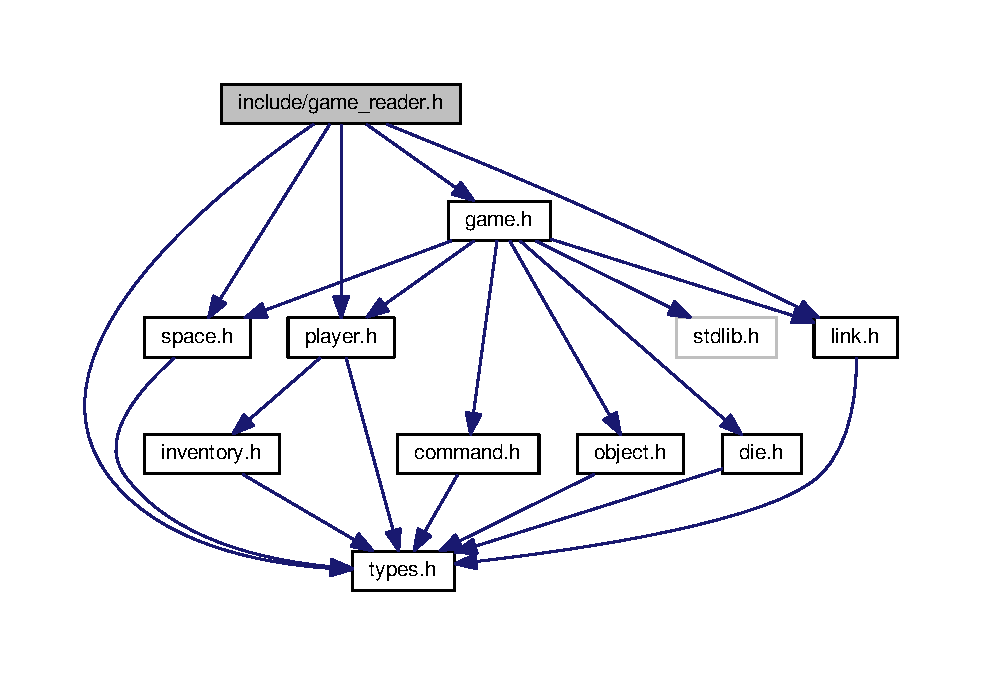
\includegraphics[width=350pt]{game__reader_8h__incl}
\end{center}
\end{figure}
\subsection*{Functions}
\begin{Indent}{\bf game\+\_\+reader\+\_\+load\+\_\+spaces}\par
{\em It loads the data of the spaces from the passed filename to the passed game.

\begin{DoxyAuthor}{Author}
Alejandro Pascual edited by Eric Morales 
\end{DoxyAuthor}
\begin{DoxyVersion}{Version}
2.\+0 
\end{DoxyVersion}
\begin{DoxyDate}{Date}
10-\/03-\/2018 
\end{DoxyDate}

\begin{DoxyParams}{Parameters}
{\em char$\ast$} & -\/$>$ a string with the name of the file containing the data of the spaces. \\
\hline
{\em Game$\ast$} & -\/$>$ a game in which the data of the spaces will be loaded. \\
\hline
\end{DoxyParams}
\begin{DoxyReturn}{Returns}
A S\+T\+A\+T\+US which indicates whether the operation could be executed correctly. 
\end{DoxyReturn}
}\begin{DoxyCompactItemize}
\item 
\hyperlink{types_8h_a32c27cc471df37f4fc818d65de0a56c4}{S\+T\+A\+T\+US} {\bfseries game\+\_\+reader\+\_\+load\+\_\+spaces} (\hyperlink{game_8h_a57156d39c530aec3fba3a9dad8c2dc6a}{Game} $\ast$, char $\ast$filename)\hypertarget{game__reader_8h_a67d68956c8a51c03d0d5b075d649c3ad}{}\label{game__reader_8h_a67d68956c8a51c03d0d5b075d649c3ad}

\end{DoxyCompactItemize}
\end{Indent}
\begin{Indent}{\bf game\+\_\+reader\+\_\+load\+\_\+players}\par
{\em It loads the data of the players from the passed filename to the passed game.

\begin{DoxyAuthor}{Author}
Eric Morales 
\end{DoxyAuthor}
\begin{DoxyVersion}{Version}
1.\+0 
\end{DoxyVersion}
\begin{DoxyDate}{Date}
26-\/03-\/2018 
\end{DoxyDate}

\begin{DoxyParams}{Parameters}
{\em char$\ast$} & -\/$>$ a string with the name of the file containing the data of the players. \\
\hline
{\em Game$\ast$} & -\/$>$ a game in which the data of the players will be loaded. \\
\hline
\end{DoxyParams}
\begin{DoxyReturn}{Returns}
A S\+T\+A\+T\+US which indicates whether the operation could be executed correctly. 
\end{DoxyReturn}
}\begin{DoxyCompactItemize}
\item 
\hyperlink{types_8h_a32c27cc471df37f4fc818d65de0a56c4}{S\+T\+A\+T\+US} {\bfseries game\+\_\+reader\+\_\+load\+\_\+players} (\hyperlink{game_8h_a57156d39c530aec3fba3a9dad8c2dc6a}{Game} $\ast$game, char $\ast$filename)\hypertarget{game__reader_8h_ab683c8c4451a43ca9639c813cadbdafc}{}\label{game__reader_8h_ab683c8c4451a43ca9639c813cadbdafc}

\end{DoxyCompactItemize}
\end{Indent}
\begin{Indent}{\bf game\+\_\+reader\+\_\+load\+\_\+objects}\par
{\em It loads the data of the objects from the passed filename to the passed game.

\begin{DoxyAuthor}{Author}
Alejandro Pascual edited by Eric Morales 
\end{DoxyAuthor}
\begin{DoxyVersion}{Version}
2.\+0 
\end{DoxyVersion}
\begin{DoxyDate}{Date}
13-\/03-\/2018 
\end{DoxyDate}

\begin{DoxyParams}{Parameters}
{\em char$\ast$} & -\/$>$ a string with the name of the file containing the data of the objects. \\
\hline
{\em Game$\ast$} & -\/$>$ a game in which the data of the objects will be loaded. \\
\hline
\end{DoxyParams}
\begin{DoxyReturn}{Returns}
A S\+T\+A\+T\+US which indicates whether the operation could be executed correctly. 
\end{DoxyReturn}
}\begin{DoxyCompactItemize}
\item 
\hyperlink{types_8h_a32c27cc471df37f4fc818d65de0a56c4}{S\+T\+A\+T\+US} {\bfseries game\+\_\+reader\+\_\+load\+\_\+objects} (\hyperlink{game_8h_a57156d39c530aec3fba3a9dad8c2dc6a}{Game} $\ast$game, char $\ast$filename)\hypertarget{game__reader_8h_a07d0cc9ec5cae35a9ad5dd7882357234}{}\label{game__reader_8h_a07d0cc9ec5cae35a9ad5dd7882357234}

\end{DoxyCompactItemize}
\end{Indent}
\begin{Indent}{\bf game\+\_\+reader\+\_\+load\+\_\+links}\par
{\em It loads the data of the links from the passed filename to the passed game.

\begin{DoxyAuthor}{Author}
Víctor Yrazusta 
\end{DoxyAuthor}
\begin{DoxyVersion}{Version}
1.\+0 
\end{DoxyVersion}
\begin{DoxyDate}{Date}
26-\/03-\/2018 
\end{DoxyDate}

\begin{DoxyParams}{Parameters}
{\em char$\ast$} & -\/$>$ a string with the name of the file containing the data of the links. \\
\hline
{\em Game$\ast$} & -\/$>$ a game in which the data of the links will be loaded. \\
\hline
\end{DoxyParams}
\begin{DoxyReturn}{Returns}
A S\+T\+A\+T\+US which indicates whether the operation could be executed correctly. 
\end{DoxyReturn}
}\begin{DoxyCompactItemize}
\item 
\hyperlink{types_8h_a32c27cc471df37f4fc818d65de0a56c4}{S\+T\+A\+T\+US} {\bfseries game\+\_\+reader\+\_\+load\+\_\+links} (\hyperlink{game_8h_a57156d39c530aec3fba3a9dad8c2dc6a}{Game} $\ast$game, char $\ast$filename)\hypertarget{game__reader_8h_aa47ab8dc1e29821281766ab359e8ac8b}{}\label{game__reader_8h_aa47ab8dc1e29821281766ab359e8ac8b}

\end{DoxyCompactItemize}
\end{Indent}


\subsection{Detailed Description}
It defines the functions to read games from files, used to initialize the game. 

\begin{DoxyAuthor}{Author}
Alejandro Pascual and Víctor Yrazusta, edited by Eric Morales 
\end{DoxyAuthor}
\begin{DoxyVersion}{Version}
1.\+0 
\end{DoxyVersion}
\begin{DoxyDate}{Date}
08-\/02-\/2018 
\end{DoxyDate}
\begin{DoxyCopyright}{Copyright}
G\+NU Public License 
\end{DoxyCopyright}

\hypertarget{game__reader__test_8h}{}\section{include/game\+\_\+reader\+\_\+test.h File Reference}
\label{game__reader__test_8h}\index{include/game\+\_\+reader\+\_\+test.\+h@{include/game\+\_\+reader\+\_\+test.\+h}}


It declares the tests for the Game Reader module.  


\subsection*{Functions}
\begin{DoxyCompactItemize}
\item 
void \hyperlink{game__reader__test_8h_a99136dde4243bfa5eaf03ef9c2716ffe}{test1\+\_\+game\+\_\+reader\+\_\+load\+\_\+spaces} ()
\item 
void \hyperlink{game__reader__test_8h_a1bf200d01046a242ee3379e62545fa01}{test2\+\_\+game\+\_\+reader\+\_\+load\+\_\+spaces} ()
\item 
void \hyperlink{game__reader__test_8h_a0a1d062789f3432e3060193f5268b5dd}{test3\+\_\+game\+\_\+reader\+\_\+load\+\_\+spaces} ()
\item 
void \hyperlink{game__reader__test_8h_af1ab6d8dc2c73b7f4902c12652e48ac6}{test4\+\_\+game\+\_\+reader\+\_\+load\+\_\+spaces} ()
\item 
void \hyperlink{game__reader__test_8h_a1f978e0818495ddc5008be23a38e5995}{test1\+\_\+game\+\_\+reader\+\_\+load\+\_\+players} ()
\item 
void \hyperlink{game__reader__test_8h_a2a92d2c5944de5ec790969ade0d10c8b}{test2\+\_\+game\+\_\+reader\+\_\+load\+\_\+players} ()
\item 
void \hyperlink{game__reader__test_8h_a8d8ffd614a258aec0e2c73172ccc7479}{test3\+\_\+game\+\_\+reader\+\_\+load\+\_\+players} ()
\item 
void \hyperlink{game__reader__test_8h_ad45fc025710a90611074500625956c3e}{test4\+\_\+game\+\_\+reader\+\_\+load\+\_\+players} ()
\item 
void \hyperlink{game__reader__test_8h_a28e7be804609ddfdf00b4798e5256030}{test1\+\_\+game\+\_\+reader\+\_\+load\+\_\+objects} ()
\item 
void \hyperlink{game__reader__test_8h_a5bd7d88df7ebba1510197eafd63a4ca3}{test2\+\_\+game\+\_\+reader\+\_\+load\+\_\+objects} ()
\item 
void \hyperlink{game__reader__test_8h_a4931f3cc77f25530c60aa5494c907e2a}{test3\+\_\+game\+\_\+reader\+\_\+load\+\_\+objects} ()
\item 
void \hyperlink{game__reader__test_8h_a91872c66040f1ad26db8460f0fe8f674}{test4\+\_\+game\+\_\+reader\+\_\+load\+\_\+objects} ()
\item 
void \hyperlink{game__reader__test_8h_aed14cf4de40dd313470f6f609e62e918}{test1\+\_\+game\+\_\+reader\+\_\+load\+\_\+links} ()
\item 
void \hyperlink{game__reader__test_8h_a7366cf536491c6f3be1145b0d7b2b32c}{test2\+\_\+game\+\_\+reader\+\_\+load\+\_\+links} ()
\item 
void \hyperlink{game__reader__test_8h_afc966d5568703a54eee14a68793ce60d}{test3\+\_\+game\+\_\+reader\+\_\+load\+\_\+links} ()
\item 
void \hyperlink{game__reader__test_8h_aeee71f446359d645ab55feb5ee3d1291}{test4\+\_\+game\+\_\+reader\+\_\+load\+\_\+links} ()
\end{DoxyCompactItemize}


\subsection{Detailed Description}
It declares the tests for the Game Reader module. 

\begin{DoxyAuthor}{Author}
Alejandro Pascual 
\end{DoxyAuthor}
\begin{DoxyVersion}{Version}
1.\+0 
\end{DoxyVersion}
\begin{DoxyDate}{Date}
07-\/04-\/2018 (creation) 
\end{DoxyDate}
\begin{DoxyCopyright}{Copyright}
G\+NU Public License 
\end{DoxyCopyright}


\subsection{Function Documentation}
\index{game\+\_\+reader\+\_\+test.\+h@{game\+\_\+reader\+\_\+test.\+h}!test1\+\_\+game\+\_\+reader\+\_\+load\+\_\+links@{test1\+\_\+game\+\_\+reader\+\_\+load\+\_\+links}}
\index{test1\+\_\+game\+\_\+reader\+\_\+load\+\_\+links@{test1\+\_\+game\+\_\+reader\+\_\+load\+\_\+links}!game\+\_\+reader\+\_\+test.\+h@{game\+\_\+reader\+\_\+test.\+h}}
\subsubsection[{\texorpdfstring{test1\+\_\+game\+\_\+reader\+\_\+load\+\_\+links()}{test1_game_reader_load_links()}}]{\setlength{\rightskip}{0pt plus 5cm}void test1\+\_\+game\+\_\+reader\+\_\+load\+\_\+links (
\begin{DoxyParamCaption}
{}
\end{DoxyParamCaption}
)}\hypertarget{game__reader__test_8h_aed14cf4de40dd313470f6f609e62e918}{}\label{game__reader__test_8h_aed14cf4de40dd313470f6f609e62e918}
\begin{DoxyRefDesc}{Test}
\item[\hyperlink{test__test000023}{Test}]Test function for loading Links \end{DoxyRefDesc}
\begin{DoxyPrecond}{Precondition}
A valid Game and a .dat with Links defined 
\end{DoxyPrecond}
\begin{DoxyPostcond}{Postcondition}
OK. The Links should be loaded in the Game 
\end{DoxyPostcond}
\index{game\+\_\+reader\+\_\+test.\+h@{game\+\_\+reader\+\_\+test.\+h}!test1\+\_\+game\+\_\+reader\+\_\+load\+\_\+objects@{test1\+\_\+game\+\_\+reader\+\_\+load\+\_\+objects}}
\index{test1\+\_\+game\+\_\+reader\+\_\+load\+\_\+objects@{test1\+\_\+game\+\_\+reader\+\_\+load\+\_\+objects}!game\+\_\+reader\+\_\+test.\+h@{game\+\_\+reader\+\_\+test.\+h}}
\subsubsection[{\texorpdfstring{test1\+\_\+game\+\_\+reader\+\_\+load\+\_\+objects()}{test1_game_reader_load_objects()}}]{\setlength{\rightskip}{0pt plus 5cm}void test1\+\_\+game\+\_\+reader\+\_\+load\+\_\+objects (
\begin{DoxyParamCaption}
{}
\end{DoxyParamCaption}
)}\hypertarget{game__reader__test_8h_a28e7be804609ddfdf00b4798e5256030}{}\label{game__reader__test_8h_a28e7be804609ddfdf00b4798e5256030}
\begin{DoxyRefDesc}{Test}
\item[\hyperlink{test__test000019}{Test}]Test function for loading Objects \end{DoxyRefDesc}
\begin{DoxyPrecond}{Precondition}
A valid Game and a .dat with Objects defined 
\end{DoxyPrecond}
\begin{DoxyPostcond}{Postcondition}
OK. The Objects should be loaded in the Game 
\end{DoxyPostcond}
\index{game\+\_\+reader\+\_\+test.\+h@{game\+\_\+reader\+\_\+test.\+h}!test1\+\_\+game\+\_\+reader\+\_\+load\+\_\+players@{test1\+\_\+game\+\_\+reader\+\_\+load\+\_\+players}}
\index{test1\+\_\+game\+\_\+reader\+\_\+load\+\_\+players@{test1\+\_\+game\+\_\+reader\+\_\+load\+\_\+players}!game\+\_\+reader\+\_\+test.\+h@{game\+\_\+reader\+\_\+test.\+h}}
\subsubsection[{\texorpdfstring{test1\+\_\+game\+\_\+reader\+\_\+load\+\_\+players()}{test1_game_reader_load_players()}}]{\setlength{\rightskip}{0pt plus 5cm}void test1\+\_\+game\+\_\+reader\+\_\+load\+\_\+players (
\begin{DoxyParamCaption}
{}
\end{DoxyParamCaption}
)}\hypertarget{game__reader__test_8h_a1f978e0818495ddc5008be23a38e5995}{}\label{game__reader__test_8h_a1f978e0818495ddc5008be23a38e5995}
\begin{DoxyRefDesc}{Test}
\item[\hyperlink{test__test000015}{Test}]Test function for loading Players \end{DoxyRefDesc}
\begin{DoxyPrecond}{Precondition}
A valid Game and a .dat with Players defined 
\end{DoxyPrecond}
\begin{DoxyPostcond}{Postcondition}
OK. The Players should be loaded in the Game 
\end{DoxyPostcond}
\index{game\+\_\+reader\+\_\+test.\+h@{game\+\_\+reader\+\_\+test.\+h}!test1\+\_\+game\+\_\+reader\+\_\+load\+\_\+spaces@{test1\+\_\+game\+\_\+reader\+\_\+load\+\_\+spaces}}
\index{test1\+\_\+game\+\_\+reader\+\_\+load\+\_\+spaces@{test1\+\_\+game\+\_\+reader\+\_\+load\+\_\+spaces}!game\+\_\+reader\+\_\+test.\+h@{game\+\_\+reader\+\_\+test.\+h}}
\subsubsection[{\texorpdfstring{test1\+\_\+game\+\_\+reader\+\_\+load\+\_\+spaces()}{test1_game_reader_load_spaces()}}]{\setlength{\rightskip}{0pt plus 5cm}void test1\+\_\+game\+\_\+reader\+\_\+load\+\_\+spaces (
\begin{DoxyParamCaption}
{}
\end{DoxyParamCaption}
)}\hypertarget{game__reader__test_8h_a99136dde4243bfa5eaf03ef9c2716ffe}{}\label{game__reader__test_8h_a99136dde4243bfa5eaf03ef9c2716ffe}
\begin{DoxyRefDesc}{Test}
\item[\hyperlink{test__test000011}{Test}]Test function for loading Spaces \end{DoxyRefDesc}
\begin{DoxyPrecond}{Precondition}
A valid Game and a .dat with Spaces defined 
\end{DoxyPrecond}
\begin{DoxyPostcond}{Postcondition}
OK. The Spaces should be loaded in the Game 
\end{DoxyPostcond}
\index{game\+\_\+reader\+\_\+test.\+h@{game\+\_\+reader\+\_\+test.\+h}!test2\+\_\+game\+\_\+reader\+\_\+load\+\_\+links@{test2\+\_\+game\+\_\+reader\+\_\+load\+\_\+links}}
\index{test2\+\_\+game\+\_\+reader\+\_\+load\+\_\+links@{test2\+\_\+game\+\_\+reader\+\_\+load\+\_\+links}!game\+\_\+reader\+\_\+test.\+h@{game\+\_\+reader\+\_\+test.\+h}}
\subsubsection[{\texorpdfstring{test2\+\_\+game\+\_\+reader\+\_\+load\+\_\+links()}{test2_game_reader_load_links()}}]{\setlength{\rightskip}{0pt plus 5cm}void test2\+\_\+game\+\_\+reader\+\_\+load\+\_\+links (
\begin{DoxyParamCaption}
{}
\end{DoxyParamCaption}
)}\hypertarget{game__reader__test_8h_a7366cf536491c6f3be1145b0d7b2b32c}{}\label{game__reader__test_8h_a7366cf536491c6f3be1145b0d7b2b32c}
\begin{DoxyRefDesc}{Test}
\item[\hyperlink{test__test000024}{Test}]Test function for loading Links \end{DoxyRefDesc}
\begin{DoxyPrecond}{Precondition}
A valid Game and a .dat with no Links defined 
\end{DoxyPrecond}
\begin{DoxyPostcond}{Postcondition}
OK. There should be no Links loaded 
\end{DoxyPostcond}
\index{game\+\_\+reader\+\_\+test.\+h@{game\+\_\+reader\+\_\+test.\+h}!test2\+\_\+game\+\_\+reader\+\_\+load\+\_\+objects@{test2\+\_\+game\+\_\+reader\+\_\+load\+\_\+objects}}
\index{test2\+\_\+game\+\_\+reader\+\_\+load\+\_\+objects@{test2\+\_\+game\+\_\+reader\+\_\+load\+\_\+objects}!game\+\_\+reader\+\_\+test.\+h@{game\+\_\+reader\+\_\+test.\+h}}
\subsubsection[{\texorpdfstring{test2\+\_\+game\+\_\+reader\+\_\+load\+\_\+objects()}{test2_game_reader_load_objects()}}]{\setlength{\rightskip}{0pt plus 5cm}void test2\+\_\+game\+\_\+reader\+\_\+load\+\_\+objects (
\begin{DoxyParamCaption}
{}
\end{DoxyParamCaption}
)}\hypertarget{game__reader__test_8h_a5bd7d88df7ebba1510197eafd63a4ca3}{}\label{game__reader__test_8h_a5bd7d88df7ebba1510197eafd63a4ca3}
\begin{DoxyRefDesc}{Test}
\item[\hyperlink{test__test000020}{Test}]Test function for loading Objects \end{DoxyRefDesc}
\begin{DoxyPrecond}{Precondition}
A valid Game and a .dat with no Objects defined 
\end{DoxyPrecond}
\begin{DoxyPostcond}{Postcondition}
OK. There should be no Objects loaded 
\end{DoxyPostcond}
\index{game\+\_\+reader\+\_\+test.\+h@{game\+\_\+reader\+\_\+test.\+h}!test2\+\_\+game\+\_\+reader\+\_\+load\+\_\+players@{test2\+\_\+game\+\_\+reader\+\_\+load\+\_\+players}}
\index{test2\+\_\+game\+\_\+reader\+\_\+load\+\_\+players@{test2\+\_\+game\+\_\+reader\+\_\+load\+\_\+players}!game\+\_\+reader\+\_\+test.\+h@{game\+\_\+reader\+\_\+test.\+h}}
\subsubsection[{\texorpdfstring{test2\+\_\+game\+\_\+reader\+\_\+load\+\_\+players()}{test2_game_reader_load_players()}}]{\setlength{\rightskip}{0pt plus 5cm}void test2\+\_\+game\+\_\+reader\+\_\+load\+\_\+players (
\begin{DoxyParamCaption}
{}
\end{DoxyParamCaption}
)}\hypertarget{game__reader__test_8h_a2a92d2c5944de5ec790969ade0d10c8b}{}\label{game__reader__test_8h_a2a92d2c5944de5ec790969ade0d10c8b}
\begin{DoxyRefDesc}{Test}
\item[\hyperlink{test__test000016}{Test}]Test function for loading Players \end{DoxyRefDesc}
\begin{DoxyPrecond}{Precondition}
A valid Game and a .dat with no Players defined 
\end{DoxyPrecond}
\begin{DoxyPostcond}{Postcondition}
OK. There should be no Players loaded 
\end{DoxyPostcond}
\index{game\+\_\+reader\+\_\+test.\+h@{game\+\_\+reader\+\_\+test.\+h}!test2\+\_\+game\+\_\+reader\+\_\+load\+\_\+spaces@{test2\+\_\+game\+\_\+reader\+\_\+load\+\_\+spaces}}
\index{test2\+\_\+game\+\_\+reader\+\_\+load\+\_\+spaces@{test2\+\_\+game\+\_\+reader\+\_\+load\+\_\+spaces}!game\+\_\+reader\+\_\+test.\+h@{game\+\_\+reader\+\_\+test.\+h}}
\subsubsection[{\texorpdfstring{test2\+\_\+game\+\_\+reader\+\_\+load\+\_\+spaces()}{test2_game_reader_load_spaces()}}]{\setlength{\rightskip}{0pt plus 5cm}void test2\+\_\+game\+\_\+reader\+\_\+load\+\_\+spaces (
\begin{DoxyParamCaption}
{}
\end{DoxyParamCaption}
)}\hypertarget{game__reader__test_8h_a1bf200d01046a242ee3379e62545fa01}{}\label{game__reader__test_8h_a1bf200d01046a242ee3379e62545fa01}
\begin{DoxyRefDesc}{Test}
\item[\hyperlink{test__test000012}{Test}]Test function for loading Spaces \end{DoxyRefDesc}
\begin{DoxyPrecond}{Precondition}
A valid Game and a .dat with no Spaces defined 
\end{DoxyPrecond}
\begin{DoxyPostcond}{Postcondition}
OK. There should be no Spaces loaded 
\end{DoxyPostcond}
\index{game\+\_\+reader\+\_\+test.\+h@{game\+\_\+reader\+\_\+test.\+h}!test3\+\_\+game\+\_\+reader\+\_\+load\+\_\+links@{test3\+\_\+game\+\_\+reader\+\_\+load\+\_\+links}}
\index{test3\+\_\+game\+\_\+reader\+\_\+load\+\_\+links@{test3\+\_\+game\+\_\+reader\+\_\+load\+\_\+links}!game\+\_\+reader\+\_\+test.\+h@{game\+\_\+reader\+\_\+test.\+h}}
\subsubsection[{\texorpdfstring{test3\+\_\+game\+\_\+reader\+\_\+load\+\_\+links()}{test3_game_reader_load_links()}}]{\setlength{\rightskip}{0pt plus 5cm}void test3\+\_\+game\+\_\+reader\+\_\+load\+\_\+links (
\begin{DoxyParamCaption}
{}
\end{DoxyParamCaption}
)}\hypertarget{game__reader__test_8h_afc966d5568703a54eee14a68793ce60d}{}\label{game__reader__test_8h_afc966d5568703a54eee14a68793ce60d}
\begin{DoxyRefDesc}{Test}
\item[\hyperlink{test__test000025}{Test}]Test function for loading Links \end{DoxyRefDesc}
\begin{DoxyPrecond}{Precondition}
An invalid Game and a valid .dat 
\end{DoxyPrecond}
\begin{DoxyPostcond}{Postcondition}
E\+R\+R\+OR 
\end{DoxyPostcond}
\index{game\+\_\+reader\+\_\+test.\+h@{game\+\_\+reader\+\_\+test.\+h}!test3\+\_\+game\+\_\+reader\+\_\+load\+\_\+objects@{test3\+\_\+game\+\_\+reader\+\_\+load\+\_\+objects}}
\index{test3\+\_\+game\+\_\+reader\+\_\+load\+\_\+objects@{test3\+\_\+game\+\_\+reader\+\_\+load\+\_\+objects}!game\+\_\+reader\+\_\+test.\+h@{game\+\_\+reader\+\_\+test.\+h}}
\subsubsection[{\texorpdfstring{test3\+\_\+game\+\_\+reader\+\_\+load\+\_\+objects()}{test3_game_reader_load_objects()}}]{\setlength{\rightskip}{0pt plus 5cm}void test3\+\_\+game\+\_\+reader\+\_\+load\+\_\+objects (
\begin{DoxyParamCaption}
{}
\end{DoxyParamCaption}
)}\hypertarget{game__reader__test_8h_a4931f3cc77f25530c60aa5494c907e2a}{}\label{game__reader__test_8h_a4931f3cc77f25530c60aa5494c907e2a}
\begin{DoxyRefDesc}{Test}
\item[\hyperlink{test__test000021}{Test}]Test function for loading Objects \end{DoxyRefDesc}
\begin{DoxyPrecond}{Precondition}
An invalid Game and a valid .dat 
\end{DoxyPrecond}
\begin{DoxyPostcond}{Postcondition}
E\+R\+R\+OR 
\end{DoxyPostcond}
\index{game\+\_\+reader\+\_\+test.\+h@{game\+\_\+reader\+\_\+test.\+h}!test3\+\_\+game\+\_\+reader\+\_\+load\+\_\+players@{test3\+\_\+game\+\_\+reader\+\_\+load\+\_\+players}}
\index{test3\+\_\+game\+\_\+reader\+\_\+load\+\_\+players@{test3\+\_\+game\+\_\+reader\+\_\+load\+\_\+players}!game\+\_\+reader\+\_\+test.\+h@{game\+\_\+reader\+\_\+test.\+h}}
\subsubsection[{\texorpdfstring{test3\+\_\+game\+\_\+reader\+\_\+load\+\_\+players()}{test3_game_reader_load_players()}}]{\setlength{\rightskip}{0pt plus 5cm}void test3\+\_\+game\+\_\+reader\+\_\+load\+\_\+players (
\begin{DoxyParamCaption}
{}
\end{DoxyParamCaption}
)}\hypertarget{game__reader__test_8h_a8d8ffd614a258aec0e2c73172ccc7479}{}\label{game__reader__test_8h_a8d8ffd614a258aec0e2c73172ccc7479}
\begin{DoxyRefDesc}{Test}
\item[\hyperlink{test__test000017}{Test}]Test function for loading Players \end{DoxyRefDesc}
\begin{DoxyPrecond}{Precondition}
An invalid Game and a valid .dat 
\end{DoxyPrecond}
\begin{DoxyPostcond}{Postcondition}
E\+R\+R\+OR 
\end{DoxyPostcond}
\index{game\+\_\+reader\+\_\+test.\+h@{game\+\_\+reader\+\_\+test.\+h}!test3\+\_\+game\+\_\+reader\+\_\+load\+\_\+spaces@{test3\+\_\+game\+\_\+reader\+\_\+load\+\_\+spaces}}
\index{test3\+\_\+game\+\_\+reader\+\_\+load\+\_\+spaces@{test3\+\_\+game\+\_\+reader\+\_\+load\+\_\+spaces}!game\+\_\+reader\+\_\+test.\+h@{game\+\_\+reader\+\_\+test.\+h}}
\subsubsection[{\texorpdfstring{test3\+\_\+game\+\_\+reader\+\_\+load\+\_\+spaces()}{test3_game_reader_load_spaces()}}]{\setlength{\rightskip}{0pt plus 5cm}void test3\+\_\+game\+\_\+reader\+\_\+load\+\_\+spaces (
\begin{DoxyParamCaption}
{}
\end{DoxyParamCaption}
)}\hypertarget{game__reader__test_8h_a0a1d062789f3432e3060193f5268b5dd}{}\label{game__reader__test_8h_a0a1d062789f3432e3060193f5268b5dd}
\begin{DoxyRefDesc}{Test}
\item[\hyperlink{test__test000013}{Test}]Test function for loading Spaces \end{DoxyRefDesc}
\begin{DoxyPrecond}{Precondition}
An invalid Game and a valid .dat 
\end{DoxyPrecond}
\begin{DoxyPostcond}{Postcondition}
E\+R\+R\+OR 
\end{DoxyPostcond}
\index{game\+\_\+reader\+\_\+test.\+h@{game\+\_\+reader\+\_\+test.\+h}!test4\+\_\+game\+\_\+reader\+\_\+load\+\_\+links@{test4\+\_\+game\+\_\+reader\+\_\+load\+\_\+links}}
\index{test4\+\_\+game\+\_\+reader\+\_\+load\+\_\+links@{test4\+\_\+game\+\_\+reader\+\_\+load\+\_\+links}!game\+\_\+reader\+\_\+test.\+h@{game\+\_\+reader\+\_\+test.\+h}}
\subsubsection[{\texorpdfstring{test4\+\_\+game\+\_\+reader\+\_\+load\+\_\+links()}{test4_game_reader_load_links()}}]{\setlength{\rightskip}{0pt plus 5cm}void test4\+\_\+game\+\_\+reader\+\_\+load\+\_\+links (
\begin{DoxyParamCaption}
{}
\end{DoxyParamCaption}
)}\hypertarget{game__reader__test_8h_aeee71f446359d645ab55feb5ee3d1291}{}\label{game__reader__test_8h_aeee71f446359d645ab55feb5ee3d1291}
\begin{DoxyRefDesc}{Test}
\item[\hyperlink{test__test000026}{Test}]Test function for loading Links \end{DoxyRefDesc}
\begin{DoxyPrecond}{Precondition}
A valid Game and an non-\/existent .dat 
\end{DoxyPrecond}
\begin{DoxyPostcond}{Postcondition}
E\+R\+R\+OR 
\end{DoxyPostcond}
\index{game\+\_\+reader\+\_\+test.\+h@{game\+\_\+reader\+\_\+test.\+h}!test4\+\_\+game\+\_\+reader\+\_\+load\+\_\+objects@{test4\+\_\+game\+\_\+reader\+\_\+load\+\_\+objects}}
\index{test4\+\_\+game\+\_\+reader\+\_\+load\+\_\+objects@{test4\+\_\+game\+\_\+reader\+\_\+load\+\_\+objects}!game\+\_\+reader\+\_\+test.\+h@{game\+\_\+reader\+\_\+test.\+h}}
\subsubsection[{\texorpdfstring{test4\+\_\+game\+\_\+reader\+\_\+load\+\_\+objects()}{test4_game_reader_load_objects()}}]{\setlength{\rightskip}{0pt plus 5cm}void test4\+\_\+game\+\_\+reader\+\_\+load\+\_\+objects (
\begin{DoxyParamCaption}
{}
\end{DoxyParamCaption}
)}\hypertarget{game__reader__test_8h_a91872c66040f1ad26db8460f0fe8f674}{}\label{game__reader__test_8h_a91872c66040f1ad26db8460f0fe8f674}
\begin{DoxyRefDesc}{Test}
\item[\hyperlink{test__test000022}{Test}]Test function for loading Objects \end{DoxyRefDesc}
\begin{DoxyPrecond}{Precondition}
A valid Game and an non-\/existent .dat 
\end{DoxyPrecond}
\begin{DoxyPostcond}{Postcondition}
E\+R\+R\+OR 
\end{DoxyPostcond}
\index{game\+\_\+reader\+\_\+test.\+h@{game\+\_\+reader\+\_\+test.\+h}!test4\+\_\+game\+\_\+reader\+\_\+load\+\_\+players@{test4\+\_\+game\+\_\+reader\+\_\+load\+\_\+players}}
\index{test4\+\_\+game\+\_\+reader\+\_\+load\+\_\+players@{test4\+\_\+game\+\_\+reader\+\_\+load\+\_\+players}!game\+\_\+reader\+\_\+test.\+h@{game\+\_\+reader\+\_\+test.\+h}}
\subsubsection[{\texorpdfstring{test4\+\_\+game\+\_\+reader\+\_\+load\+\_\+players()}{test4_game_reader_load_players()}}]{\setlength{\rightskip}{0pt plus 5cm}void test4\+\_\+game\+\_\+reader\+\_\+load\+\_\+players (
\begin{DoxyParamCaption}
{}
\end{DoxyParamCaption}
)}\hypertarget{game__reader__test_8h_ad45fc025710a90611074500625956c3e}{}\label{game__reader__test_8h_ad45fc025710a90611074500625956c3e}
\begin{DoxyRefDesc}{Test}
\item[\hyperlink{test__test000018}{Test}]Test function for loading Players \end{DoxyRefDesc}
\begin{DoxyPrecond}{Precondition}
A valid Game and an non-\/existent .dat 
\end{DoxyPrecond}
\begin{DoxyPostcond}{Postcondition}
E\+R\+R\+OR 
\end{DoxyPostcond}
\index{game\+\_\+reader\+\_\+test.\+h@{game\+\_\+reader\+\_\+test.\+h}!test4\+\_\+game\+\_\+reader\+\_\+load\+\_\+spaces@{test4\+\_\+game\+\_\+reader\+\_\+load\+\_\+spaces}}
\index{test4\+\_\+game\+\_\+reader\+\_\+load\+\_\+spaces@{test4\+\_\+game\+\_\+reader\+\_\+load\+\_\+spaces}!game\+\_\+reader\+\_\+test.\+h@{game\+\_\+reader\+\_\+test.\+h}}
\subsubsection[{\texorpdfstring{test4\+\_\+game\+\_\+reader\+\_\+load\+\_\+spaces()}{test4_game_reader_load_spaces()}}]{\setlength{\rightskip}{0pt plus 5cm}void test4\+\_\+game\+\_\+reader\+\_\+load\+\_\+spaces (
\begin{DoxyParamCaption}
{}
\end{DoxyParamCaption}
)}\hypertarget{game__reader__test_8h_af1ab6d8dc2c73b7f4902c12652e48ac6}{}\label{game__reader__test_8h_af1ab6d8dc2c73b7f4902c12652e48ac6}
\begin{DoxyRefDesc}{Test}
\item[\hyperlink{test__test000014}{Test}]Test function for loading Spaces \end{DoxyRefDesc}
\begin{DoxyPrecond}{Precondition}
A valid Game and an non-\/existent .dat 
\end{DoxyPrecond}
\begin{DoxyPostcond}{Postcondition}
E\+R\+R\+OR 
\end{DoxyPostcond}

\hypertarget{game__test_8h}{}\section{include/game\+\_\+test.h File Reference}
\label{game__test_8h}\index{include/game\+\_\+test.\+h@{include/game\+\_\+test.\+h}}


It declares the tests for the game module.  


\subsection*{Functions}
\begin{DoxyCompactItemize}
\item 
void \hyperlink{game__test_8h_a1d5c70cf073b025bb5d74413cecd929b}{test1\+\_\+game\+\_\+create} ()
\item 
void \hyperlink{game__test_8h_a867d2e7bebdfa55ee8b8a73764c46f5b}{test1\+\_\+game\+\_\+create\+\_\+from\+\_\+file} ()
\item 
void \hyperlink{game__test_8h_ad6ce67f6184f6ead2aaca860f64e9b76}{test2\+\_\+game\+\_\+create\+\_\+from\+\_\+file} ()
\item 
void \hyperlink{game__test_8h_a7f6e56d152bfbaab1aa140f7bf6494a1}{test3\+\_\+game\+\_\+create\+\_\+from\+\_\+file} ()
\item 
void \hyperlink{game__test_8h_aa6087c9d179d02f0fb7a5f1d0a13cffe}{test4\+\_\+game\+\_\+create\+\_\+from\+\_\+file} ()
\item 
void \hyperlink{game__test_8h_acef689d23c451c738aab116984001501}{test1\+\_\+game\+\_\+update} ()
\item 
void \hyperlink{game__test_8h_aa7c7e1467a24f4d1086096b73a38739e}{test2\+\_\+game\+\_\+update} ()
\item 
void \hyperlink{game__test_8h_abb9b53b5dbd1f36a9518e11c0a0bee16}{test1\+\_\+game\+\_\+destroy} ()
\item 
void \hyperlink{game__test_8h_a91a33a9fce738616f2140d06a6ff079f}{test2\+\_\+game\+\_\+destroy} ()
\item 
void \hyperlink{game__test_8h_a6ab3378c3e627b8ff5cb397ecb46d268}{test1\+\_\+game\+\_\+is\+\_\+over} ()
\item 
void \hyperlink{game__test_8h_aad6c50be5f1d541ca5414b86558ef422}{test2\+\_\+game\+\_\+is\+\_\+over} ()
\item 
void \hyperlink{game__test_8h_a49b59f8e75a8a4375c98ded865f16fcc}{test1\+\_\+game\+\_\+add\+\_\+space} ()
\item 
void \hyperlink{game__test_8h_aed0f40f3ab1c252e548b038542d7409d}{test2\+\_\+game\+\_\+add\+\_\+space} ()
\item 
void \hyperlink{game__test_8h_a7d77ce55d38ea58e076f160dc0ea019c}{test3\+\_\+game\+\_\+add\+\_\+space} ()
\item 
void \hyperlink{game__test_8h_a1cd2a0a0c093a5144ed375760b7dc10f}{test4\+\_\+game\+\_\+add\+\_\+space} ()
\item 
void \hyperlink{game__test_8h_a4adb115e4624c38738c938b999f6c949}{test1\+\_\+game\+\_\+add\+\_\+player} ()
\item 
void \hyperlink{game__test_8h_a42bb53c500bf8ae4dce0e144a85cd80b}{test2\+\_\+game\+\_\+add\+\_\+player} ()
\item 
void \hyperlink{game__test_8h_aae8f72a6c0030f8ecf6b27e8cc218d08}{test3\+\_\+game\+\_\+add\+\_\+player} ()
\item 
void \hyperlink{game__test_8h_a5f21b1b7e92b85990d3e5f4ea82ba68e}{test4\+\_\+game\+\_\+add\+\_\+player} ()
\item 
void \hyperlink{game__test_8h_a2a13a20e66d04d3d99812ad9b331a912}{test5\+\_\+game\+\_\+add\+\_\+player} ()
\item 
void \hyperlink{game__test_8h_ac60415277fc72d0a231b17e482a6609b}{test1\+\_\+game\+\_\+add\+\_\+object} ()
\item 
void \hyperlink{game__test_8h_ab996895e69c5d41fab5515e88aed3975}{test2\+\_\+game\+\_\+add\+\_\+object} ()
\item 
void \hyperlink{game__test_8h_ac6b7f7180414f14b0ca9629999da9f75}{test3\+\_\+game\+\_\+add\+\_\+object} ()
\item 
void \hyperlink{game__test_8h_a5384fe9237e9434f5d1e80fc00380721}{test4\+\_\+game\+\_\+add\+\_\+object} ()
\item 
void \hyperlink{game__test_8h_adeda95b2589eb0d71bf75fb8d567b51a}{test5\+\_\+game\+\_\+add\+\_\+object} ()
\item 
void \hyperlink{game__test_8h_a6e0bfd68c1415964c3cd0e03bbcc1acb}{test6\+\_\+game\+\_\+add\+\_\+object} ()
\item 
void \hyperlink{game__test_8h_ab8c2b4ef2ac2319b3d039e3775f6ce34}{test1\+\_\+game\+\_\+get\+\_\+spaces\+\_\+number} ()
\item 
void \hyperlink{game__test_8h_ae8acea54aeabc7ca6bb3f4ccb7019947}{test2\+\_\+game\+\_\+get\+\_\+spaces\+\_\+number} ()
\item 
void \hyperlink{game__test_8h_aa1f4bf660db3c61f70d3c96cb0c1a3e8}{test3\+\_\+game\+\_\+get\+\_\+spaces\+\_\+number} ()
\item 
void \hyperlink{game__test_8h_ae33709bf82f1ddc9b8a06176c97de56c}{test4\+\_\+game\+\_\+get\+\_\+spaces\+\_\+number} ()
\item 
void \hyperlink{game__test_8h_af8bec2d2267ab511ba4c3d0a3fa46622}{test1\+\_\+game\+\_\+get\+\_\+players\+\_\+number} ()
\item 
void \hyperlink{game__test_8h_a2a530a4de5f42cebd34d3a2b13b571b3}{test2\+\_\+game\+\_\+get\+\_\+players\+\_\+number} ()
\item 
void \hyperlink{game__test_8h_aea376050c113263f20a53d26b951be06}{test3\+\_\+game\+\_\+get\+\_\+players\+\_\+number} ()
\item 
void \hyperlink{game__test_8h_a0147e621a4267900f75e271170104872}{test4\+\_\+game\+\_\+get\+\_\+players\+\_\+number} ()
\item 
void \hyperlink{game__test_8h_a1649f86f3414e97a09b230bae2b9911b}{test1\+\_\+game\+\_\+get\+\_\+objects\+\_\+number} ()
\item 
void \hyperlink{game__test_8h_a666e45de68b2bbc214dbd1c7f0cbc1ff}{test2\+\_\+game\+\_\+get\+\_\+objects\+\_\+number} ()
\item 
void \hyperlink{game__test_8h_a0ffd506d0a39ef21dd95674bab10db41}{test3\+\_\+game\+\_\+get\+\_\+objects\+\_\+number} ()
\item 
void \hyperlink{game__test_8h_a4186bf1b76d8e7ed80fb05b0947f9a1e}{test4\+\_\+game\+\_\+get\+\_\+objects\+\_\+number} ()
\item 
void \hyperlink{game__test_8h_a7d3e65d6960a38ca883d0591a679f9c4}{test1\+\_\+game\+\_\+get\+\_\+dies\+\_\+number} ()
\item 
void \hyperlink{game__test_8h_a3cf79c20d8101232319754300c699a22}{test2\+\_\+game\+\_\+get\+\_\+dies\+\_\+number} ()
\item 
void \hyperlink{game__test_8h_a6c4aa8df2680e65915e1c9b687164028}{test1\+\_\+game\+\_\+find} ()
\item 
void \hyperlink{game__test_8h_a5894e9abe6b633d53b01ad8691655a26}{test2\+\_\+game\+\_\+find} ()
\item 
void \hyperlink{game__test_8h_aa2d9c89ee35519890e43765fc1fc1277}{test3\+\_\+game\+\_\+find} ()
\item 
void \hyperlink{game__test_8h_acf41e567400a66fca3a2c1224aa44de9}{test1\+\_\+game\+\_\+find\+\_\+name} ()
\item 
void \hyperlink{game__test_8h_a4a26a36f14da83a296ff5057ddfd67a7}{test2\+\_\+game\+\_\+find\+\_\+name} ()
\item 
void \hyperlink{game__test_8h_a36c785fccb9a27f47e0e8a75b95ca465}{test3\+\_\+game\+\_\+find\+\_\+name} ()
\item 
void \hyperlink{game__test_8h_a467fe2bad25b7d53fa51ad3901f4672f}{test1\+\_\+game\+\_\+set\+\_\+object\+\_\+location} ()
\item 
void \hyperlink{game__test_8h_a2bee8c4494438aa5cdc301ca6ef40e88}{test2\+\_\+game\+\_\+set\+\_\+object\+\_\+location} ()
\item 
void \hyperlink{game__test_8h_a2eb1b65a3a2adf0a890377debabbf265}{test3\+\_\+game\+\_\+set\+\_\+object\+\_\+location} ()
\item 
void \hyperlink{game__test_8h_ac94ee201653d62006bc315592236ac90}{test4\+\_\+game\+\_\+set\+\_\+object\+\_\+location} ()
\item 
void \hyperlink{game__test_8h_adffc2120d97aef04f9387431397defbc}{test1\+\_\+game\+\_\+get\+\_\+last\+\_\+command} ()
\item 
void \hyperlink{game__test_8h_ac6463a36d0a06d720225b64f894ec445}{test2\+\_\+game\+\_\+get\+\_\+last\+\_\+command} ()
\item 
void \hyperlink{game__test_8h_a2eb3d363edd323ead30c8392366e2fa9}{test1\+\_\+game\+\_\+get\+\_\+status\+\_\+last\+\_\+command} ()
\item 
void \hyperlink{game__test_8h_a5828e75b146cd90e87938d17f5c0c114}{test2\+\_\+game\+\_\+get\+\_\+status\+\_\+last\+\_\+command} ()
\item 
void \hyperlink{game__test_8h_a979cf97b28d14da099d77631877101ef}{test1\+\_\+game\+\_\+get\+\_\+last\+\_\+check} ()
\item 
void \hyperlink{game__test_8h_af601b07387856d9fbf5fb30eaae11191}{test2\+\_\+game\+\_\+get\+\_\+last\+\_\+check} ()
\item 
void \hyperlink{game__test_8h_a05b101ce9a7d4c4599f13547de2ded54}{test3\+\_\+game\+\_\+get\+\_\+last\+\_\+check} ()
\item 
void \hyperlink{game__test_8h_ab936ab03dff02b8edde97651f12384ea}{test1\+\_\+game\+\_\+add\+\_\+link} ()
\item 
void \hyperlink{game__test_8h_af5c4dd79b2a7b67adbeeb8df5791a5de}{test2\+\_\+game\+\_\+add\+\_\+link} ()
\item 
void \hyperlink{game__test_8h_af97f3fbab50d8122acc5b2632c9a27cb}{test3\+\_\+game\+\_\+add\+\_\+link} ()
\end{DoxyCompactItemize}


\subsection{Detailed Description}
It declares the tests for the game module. 

\begin{DoxyAuthor}{Author}
Javier Lougedo 
\end{DoxyAuthor}
\begin{DoxyVersion}{Version}
2.\+0 
\end{DoxyVersion}
\begin{DoxyDate}{Date}
19-\/01-\/2016 
\end{DoxyDate}
\begin{DoxyCopyright}{Copyright}
G\+NU Public License 
\end{DoxyCopyright}


\subsection{Function Documentation}
\index{game\+\_\+test.\+h@{game\+\_\+test.\+h}!test1\+\_\+game\+\_\+add\+\_\+link@{test1\+\_\+game\+\_\+add\+\_\+link}}
\index{test1\+\_\+game\+\_\+add\+\_\+link@{test1\+\_\+game\+\_\+add\+\_\+link}!game\+\_\+test.\+h@{game\+\_\+test.\+h}}
\subsubsection[{\texorpdfstring{test1\+\_\+game\+\_\+add\+\_\+link()}{test1_game_add_link()}}]{\setlength{\rightskip}{0pt plus 5cm}void test1\+\_\+game\+\_\+add\+\_\+link (
\begin{DoxyParamCaption}
{}
\end{DoxyParamCaption}
)}\hypertarget{game__test_8h_ab936ab03dff02b8edde97651f12384ea}{}\label{game__test_8h_ab936ab03dff02b8edde97651f12384ea}
\begin{DoxyRefDesc}{Test}
\item[\hyperlink{test__test000085}{Test}]Test with normal conditions \end{DoxyRefDesc}
\begin{DoxyPrecond}{Precondition}
Created Game and a Link to add 
\end{DoxyPrecond}
\begin{DoxyPostcond}{Postcondition}
O\+U\+T\+P\+UT==OK 
\end{DoxyPostcond}
\index{game\+\_\+test.\+h@{game\+\_\+test.\+h}!test1\+\_\+game\+\_\+add\+\_\+object@{test1\+\_\+game\+\_\+add\+\_\+object}}
\index{test1\+\_\+game\+\_\+add\+\_\+object@{test1\+\_\+game\+\_\+add\+\_\+object}!game\+\_\+test.\+h@{game\+\_\+test.\+h}}
\subsubsection[{\texorpdfstring{test1\+\_\+game\+\_\+add\+\_\+object()}{test1_game_add_object()}}]{\setlength{\rightskip}{0pt plus 5cm}void test1\+\_\+game\+\_\+add\+\_\+object (
\begin{DoxyParamCaption}
{}
\end{DoxyParamCaption}
)}\hypertarget{game__test_8h_ac60415277fc72d0a231b17e482a6609b}{}\label{game__test_8h_ac60415277fc72d0a231b17e482a6609b}
\begin{DoxyRefDesc}{Test}
\item[\hyperlink{test__test000047}{Test}]Test to see if adding objects normally works correctly \end{DoxyRefDesc}
\begin{DoxyPrecond}{Precondition}
Created Game, an Object and a location Id 
\end{DoxyPrecond}
\begin{DoxyPostcond}{Postcondition}
O\+U\+T\+P\+UT==OK 
\end{DoxyPostcond}
\index{game\+\_\+test.\+h@{game\+\_\+test.\+h}!test1\+\_\+game\+\_\+add\+\_\+player@{test1\+\_\+game\+\_\+add\+\_\+player}}
\index{test1\+\_\+game\+\_\+add\+\_\+player@{test1\+\_\+game\+\_\+add\+\_\+player}!game\+\_\+test.\+h@{game\+\_\+test.\+h}}
\subsubsection[{\texorpdfstring{test1\+\_\+game\+\_\+add\+\_\+player()}{test1_game_add_player()}}]{\setlength{\rightskip}{0pt plus 5cm}void test1\+\_\+game\+\_\+add\+\_\+player (
\begin{DoxyParamCaption}
{}
\end{DoxyParamCaption}
)}\hypertarget{game__test_8h_a4adb115e4624c38738c938b999f6c949}{}\label{game__test_8h_a4adb115e4624c38738c938b999f6c949}
\begin{DoxyRefDesc}{Test}
\item[\hyperlink{test__test000042}{Test}]Test with normal conditions \end{DoxyRefDesc}
\begin{DoxyPrecond}{Precondition}
Created Game a Player and a location 
\end{DoxyPrecond}
\begin{DoxyPostcond}{Postcondition}
O\+U\+T\+P\+UT==OK 
\end{DoxyPostcond}
\index{game\+\_\+test.\+h@{game\+\_\+test.\+h}!test1\+\_\+game\+\_\+add\+\_\+space@{test1\+\_\+game\+\_\+add\+\_\+space}}
\index{test1\+\_\+game\+\_\+add\+\_\+space@{test1\+\_\+game\+\_\+add\+\_\+space}!game\+\_\+test.\+h@{game\+\_\+test.\+h}}
\subsubsection[{\texorpdfstring{test1\+\_\+game\+\_\+add\+\_\+space()}{test1_game_add_space()}}]{\setlength{\rightskip}{0pt plus 5cm}void test1\+\_\+game\+\_\+add\+\_\+space (
\begin{DoxyParamCaption}
{}
\end{DoxyParamCaption}
)}\hypertarget{game__test_8h_a49b59f8e75a8a4375c98ded865f16fcc}{}\label{game__test_8h_a49b59f8e75a8a4375c98ded865f16fcc}
\begin{DoxyRefDesc}{Test}
\item[\hyperlink{test__test000038}{Test}]Test to see if adding spaces works correctly \end{DoxyRefDesc}
\begin{DoxyPrecond}{Precondition}
Created Game and Space Id 
\end{DoxyPrecond}
\begin{DoxyPostcond}{Postcondition}
O\+U\+T\+P\+UT==OK 
\end{DoxyPostcond}
\index{game\+\_\+test.\+h@{game\+\_\+test.\+h}!test1\+\_\+game\+\_\+create@{test1\+\_\+game\+\_\+create}}
\index{test1\+\_\+game\+\_\+create@{test1\+\_\+game\+\_\+create}!game\+\_\+test.\+h@{game\+\_\+test.\+h}}
\subsubsection[{\texorpdfstring{test1\+\_\+game\+\_\+create()}{test1_game_create()}}]{\setlength{\rightskip}{0pt plus 5cm}void test1\+\_\+game\+\_\+create (
\begin{DoxyParamCaption}
{}
\end{DoxyParamCaption}
)}\hypertarget{game__test_8h_a1d5c70cf073b025bb5d74413cecd929b}{}\label{game__test_8h_a1d5c70cf073b025bb5d74413cecd929b}
\begin{DoxyRefDesc}{Test}
\item[\hyperlink{test__test000027}{Test}]Test to see if game\+\_\+create works correctly \end{DoxyRefDesc}
\begin{DoxyPrecond}{Precondition}
N\+U\+LL Game 
\end{DoxyPrecond}
\begin{DoxyPostcond}{Postcondition}
Should return a created game (different from N\+U\+LL) 
\end{DoxyPostcond}
\index{game\+\_\+test.\+h@{game\+\_\+test.\+h}!test1\+\_\+game\+\_\+create\+\_\+from\+\_\+file@{test1\+\_\+game\+\_\+create\+\_\+from\+\_\+file}}
\index{test1\+\_\+game\+\_\+create\+\_\+from\+\_\+file@{test1\+\_\+game\+\_\+create\+\_\+from\+\_\+file}!game\+\_\+test.\+h@{game\+\_\+test.\+h}}
\subsubsection[{\texorpdfstring{test1\+\_\+game\+\_\+create\+\_\+from\+\_\+file()}{test1_game_create_from_file()}}]{\setlength{\rightskip}{0pt plus 5cm}void test1\+\_\+game\+\_\+create\+\_\+from\+\_\+file (
\begin{DoxyParamCaption}
{}
\end{DoxyParamCaption}
)}\hypertarget{game__test_8h_a867d2e7bebdfa55ee8b8a73764c46f5b}{}\label{game__test_8h_a867d2e7bebdfa55ee8b8a73764c46f5b}
\begin{DoxyRefDesc}{Test}
\item[\hyperlink{test__test000028}{Test}]Test to check if a game is created correctly from a file. \end{DoxyRefDesc}
\begin{DoxyPrecond}{Precondition}
Created Game and a data file 
\end{DoxyPrecond}
\begin{DoxyPostcond}{Postcondition}
O\+U\+T\+P\+UT==OK 
\end{DoxyPostcond}
\index{game\+\_\+test.\+h@{game\+\_\+test.\+h}!test1\+\_\+game\+\_\+destroy@{test1\+\_\+game\+\_\+destroy}}
\index{test1\+\_\+game\+\_\+destroy@{test1\+\_\+game\+\_\+destroy}!game\+\_\+test.\+h@{game\+\_\+test.\+h}}
\subsubsection[{\texorpdfstring{test1\+\_\+game\+\_\+destroy()}{test1_game_destroy()}}]{\setlength{\rightskip}{0pt plus 5cm}void test1\+\_\+game\+\_\+destroy (
\begin{DoxyParamCaption}
{}
\end{DoxyParamCaption}
)}\hypertarget{game__test_8h_abb9b53b5dbd1f36a9518e11c0a0bee16}{}\label{game__test_8h_abb9b53b5dbd1f36a9518e11c0a0bee16}
\begin{DoxyRefDesc}{Test}
\item[\hyperlink{test__test000034}{Test}]Test if game destroys a created Game. \end{DoxyRefDesc}
\begin{DoxyPrecond}{Precondition}
Created Game 
\end{DoxyPrecond}
\begin{DoxyPostcond}{Postcondition}
O\+U\+T\+P\+UT==OK 
\end{DoxyPostcond}
\index{game\+\_\+test.\+h@{game\+\_\+test.\+h}!test1\+\_\+game\+\_\+find@{test1\+\_\+game\+\_\+find}}
\index{test1\+\_\+game\+\_\+find@{test1\+\_\+game\+\_\+find}!game\+\_\+test.\+h@{game\+\_\+test.\+h}}
\subsubsection[{\texorpdfstring{test1\+\_\+game\+\_\+find()}{test1_game_find()}}]{\setlength{\rightskip}{0pt plus 5cm}void test1\+\_\+game\+\_\+find (
\begin{DoxyParamCaption}
{}
\end{DoxyParamCaption}
)}\hypertarget{game__test_8h_a6c4aa8df2680e65915e1c9b687164028}{}\label{game__test_8h_a6c4aa8df2680e65915e1c9b687164028}
\begin{DoxyRefDesc}{Test}
\item[\hyperlink{test__test000067}{Test}]Test to see if it works normally \end{DoxyRefDesc}
\begin{DoxyPrecond}{Precondition}
Created Game. 
\end{DoxyPrecond}
\begin{DoxyPostcond}{Postcondition}
O\+U\+T\+P\+UT not N\+U\+LL 
\end{DoxyPostcond}
\index{game\+\_\+test.\+h@{game\+\_\+test.\+h}!test1\+\_\+game\+\_\+find\+\_\+name@{test1\+\_\+game\+\_\+find\+\_\+name}}
\index{test1\+\_\+game\+\_\+find\+\_\+name@{test1\+\_\+game\+\_\+find\+\_\+name}!game\+\_\+test.\+h@{game\+\_\+test.\+h}}
\subsubsection[{\texorpdfstring{test1\+\_\+game\+\_\+find\+\_\+name()}{test1_game_find_name()}}]{\setlength{\rightskip}{0pt plus 5cm}void test1\+\_\+game\+\_\+find\+\_\+name (
\begin{DoxyParamCaption}
{}
\end{DoxyParamCaption}
)}\hypertarget{game__test_8h_acf41e567400a66fca3a2c1224aa44de9}{}\label{game__test_8h_acf41e567400a66fca3a2c1224aa44de9}
\begin{DoxyRefDesc}{Test}
\item[\hyperlink{test__test000070}{Test}]Test to see if it works normally \end{DoxyRefDesc}
\begin{DoxyPrecond}{Precondition}
Created Game. 
\end{DoxyPrecond}
\begin{DoxyPostcond}{Postcondition}
O\+U\+T\+P\+UT not N\+U\+LL 
\end{DoxyPostcond}
\index{game\+\_\+test.\+h@{game\+\_\+test.\+h}!test1\+\_\+game\+\_\+get\+\_\+dies\+\_\+number@{test1\+\_\+game\+\_\+get\+\_\+dies\+\_\+number}}
\index{test1\+\_\+game\+\_\+get\+\_\+dies\+\_\+number@{test1\+\_\+game\+\_\+get\+\_\+dies\+\_\+number}!game\+\_\+test.\+h@{game\+\_\+test.\+h}}
\subsubsection[{\texorpdfstring{test1\+\_\+game\+\_\+get\+\_\+dies\+\_\+number()}{test1_game_get_dies_number()}}]{\setlength{\rightskip}{0pt plus 5cm}void test1\+\_\+game\+\_\+get\+\_\+dies\+\_\+number (
\begin{DoxyParamCaption}
{}
\end{DoxyParamCaption}
)}\hypertarget{game__test_8h_a7d3e65d6960a38ca883d0591a679f9c4}{}\label{game__test_8h_a7d3e65d6960a38ca883d0591a679f9c4}
\begin{DoxyRefDesc}{Test}
\item[\hyperlink{test__test000065}{Test}]Test to see if the number (0) of returned dies is correct. \end{DoxyRefDesc}
\begin{DoxyPrecond}{Precondition}
Created Game 
\end{DoxyPrecond}
\begin{DoxyPostcond}{Postcondition}
O\+U\+T\+P\+UT==0 
\end{DoxyPostcond}
\index{game\+\_\+test.\+h@{game\+\_\+test.\+h}!test1\+\_\+game\+\_\+get\+\_\+last\+\_\+check@{test1\+\_\+game\+\_\+get\+\_\+last\+\_\+check}}
\index{test1\+\_\+game\+\_\+get\+\_\+last\+\_\+check@{test1\+\_\+game\+\_\+get\+\_\+last\+\_\+check}!game\+\_\+test.\+h@{game\+\_\+test.\+h}}
\subsubsection[{\texorpdfstring{test1\+\_\+game\+\_\+get\+\_\+last\+\_\+check()}{test1_game_get_last_check()}}]{\setlength{\rightskip}{0pt plus 5cm}void test1\+\_\+game\+\_\+get\+\_\+last\+\_\+check (
\begin{DoxyParamCaption}
{}
\end{DoxyParamCaption}
)}\hypertarget{game__test_8h_a979cf97b28d14da099d77631877101ef}{}\label{game__test_8h_a979cf97b28d14da099d77631877101ef}
\begin{DoxyRefDesc}{Test}
\item[\hyperlink{test__test000082}{Test}]Test to see if works in normal conditions with an object \end{DoxyRefDesc}
\begin{DoxyPrecond}{Precondition}
Created Game 
\end{DoxyPrecond}
\begin{DoxyPostcond}{Postcondition}
O\+U\+T\+P\+UT==O\+B\+J\+\_\+\+D\+E\+SC 
\end{DoxyPostcond}
\index{game\+\_\+test.\+h@{game\+\_\+test.\+h}!test1\+\_\+game\+\_\+get\+\_\+last\+\_\+command@{test1\+\_\+game\+\_\+get\+\_\+last\+\_\+command}}
\index{test1\+\_\+game\+\_\+get\+\_\+last\+\_\+command@{test1\+\_\+game\+\_\+get\+\_\+last\+\_\+command}!game\+\_\+test.\+h@{game\+\_\+test.\+h}}
\subsubsection[{\texorpdfstring{test1\+\_\+game\+\_\+get\+\_\+last\+\_\+command()}{test1_game_get_last_command()}}]{\setlength{\rightskip}{0pt plus 5cm}void test1\+\_\+game\+\_\+get\+\_\+last\+\_\+command (
\begin{DoxyParamCaption}
{}
\end{DoxyParamCaption}
)}\hypertarget{game__test_8h_adffc2120d97aef04f9387431397defbc}{}\label{game__test_8h_adffc2120d97aef04f9387431397defbc}
\begin{DoxyRefDesc}{Test}
\item[\hyperlink{test__test000078}{Test}]Test to see if works in normal conditions \end{DoxyRefDesc}
\begin{DoxyPrecond}{Precondition}
Created Game with grasp command 
\end{DoxyPrecond}
\begin{DoxyPostcond}{Postcondition}
O\+U\+T\+P\+UT==G\+R\+A\+SP 
\end{DoxyPostcond}
\index{game\+\_\+test.\+h@{game\+\_\+test.\+h}!test1\+\_\+game\+\_\+get\+\_\+objects\+\_\+number@{test1\+\_\+game\+\_\+get\+\_\+objects\+\_\+number}}
\index{test1\+\_\+game\+\_\+get\+\_\+objects\+\_\+number@{test1\+\_\+game\+\_\+get\+\_\+objects\+\_\+number}!game\+\_\+test.\+h@{game\+\_\+test.\+h}}
\subsubsection[{\texorpdfstring{test1\+\_\+game\+\_\+get\+\_\+objects\+\_\+number()}{test1_game_get_objects_number()}}]{\setlength{\rightskip}{0pt plus 5cm}void test1\+\_\+game\+\_\+get\+\_\+objects\+\_\+number (
\begin{DoxyParamCaption}
{}
\end{DoxyParamCaption}
)}\hypertarget{game__test_8h_a1649f86f3414e97a09b230bae2b9911b}{}\label{game__test_8h_a1649f86f3414e97a09b230bae2b9911b}
\begin{DoxyRefDesc}{Test}
\item[\hyperlink{test__test000061}{Test}]Test to see if the number (1) of returned objects is correct. \end{DoxyRefDesc}
\begin{DoxyPrecond}{Precondition}
Created Game and a object 
\end{DoxyPrecond}
\begin{DoxyPostcond}{Postcondition}
O\+U\+T\+P\+UT==1 
\end{DoxyPostcond}
\index{game\+\_\+test.\+h@{game\+\_\+test.\+h}!test1\+\_\+game\+\_\+get\+\_\+players\+\_\+number@{test1\+\_\+game\+\_\+get\+\_\+players\+\_\+number}}
\index{test1\+\_\+game\+\_\+get\+\_\+players\+\_\+number@{test1\+\_\+game\+\_\+get\+\_\+players\+\_\+number}!game\+\_\+test.\+h@{game\+\_\+test.\+h}}
\subsubsection[{\texorpdfstring{test1\+\_\+game\+\_\+get\+\_\+players\+\_\+number()}{test1_game_get_players_number()}}]{\setlength{\rightskip}{0pt plus 5cm}void test1\+\_\+game\+\_\+get\+\_\+players\+\_\+number (
\begin{DoxyParamCaption}
{}
\end{DoxyParamCaption}
)}\hypertarget{game__test_8h_af8bec2d2267ab511ba4c3d0a3fa46622}{}\label{game__test_8h_af8bec2d2267ab511ba4c3d0a3fa46622}
\begin{DoxyRefDesc}{Test}
\item[\hyperlink{test__test000057}{Test}]Test to see if the number (1) of returned players is correct. \end{DoxyRefDesc}
\begin{DoxyPrecond}{Precondition}
Created Game and a Player 
\end{DoxyPrecond}
\begin{DoxyPostcond}{Postcondition}
O\+U\+T\+P\+UT==1 
\end{DoxyPostcond}
\index{game\+\_\+test.\+h@{game\+\_\+test.\+h}!test1\+\_\+game\+\_\+get\+\_\+spaces\+\_\+number@{test1\+\_\+game\+\_\+get\+\_\+spaces\+\_\+number}}
\index{test1\+\_\+game\+\_\+get\+\_\+spaces\+\_\+number@{test1\+\_\+game\+\_\+get\+\_\+spaces\+\_\+number}!game\+\_\+test.\+h@{game\+\_\+test.\+h}}
\subsubsection[{\texorpdfstring{test1\+\_\+game\+\_\+get\+\_\+spaces\+\_\+number()}{test1_game_get_spaces_number()}}]{\setlength{\rightskip}{0pt plus 5cm}void test1\+\_\+game\+\_\+get\+\_\+spaces\+\_\+number (
\begin{DoxyParamCaption}
{}
\end{DoxyParamCaption}
)}\hypertarget{game__test_8h_ab8c2b4ef2ac2319b3d039e3775f6ce34}{}\label{game__test_8h_ab8c2b4ef2ac2319b3d039e3775f6ce34}
\begin{DoxyRefDesc}{Test}
\item[\hyperlink{test__test000053}{Test}]Test to see if the number (1) of returned spaces is correct. \end{DoxyRefDesc}
\begin{DoxyPrecond}{Precondition}
Created Game and a Space 
\end{DoxyPrecond}
\begin{DoxyPostcond}{Postcondition}
O\+U\+T\+P\+UT==1 
\end{DoxyPostcond}
\index{game\+\_\+test.\+h@{game\+\_\+test.\+h}!test1\+\_\+game\+\_\+get\+\_\+status\+\_\+last\+\_\+command@{test1\+\_\+game\+\_\+get\+\_\+status\+\_\+last\+\_\+command}}
\index{test1\+\_\+game\+\_\+get\+\_\+status\+\_\+last\+\_\+command@{test1\+\_\+game\+\_\+get\+\_\+status\+\_\+last\+\_\+command}!game\+\_\+test.\+h@{game\+\_\+test.\+h}}
\subsubsection[{\texorpdfstring{test1\+\_\+game\+\_\+get\+\_\+status\+\_\+last\+\_\+command()}{test1_game_get_status_last_command()}}]{\setlength{\rightskip}{0pt plus 5cm}void test1\+\_\+game\+\_\+get\+\_\+status\+\_\+last\+\_\+command (
\begin{DoxyParamCaption}
{}
\end{DoxyParamCaption}
)}\hypertarget{game__test_8h_a2eb3d363edd323ead30c8392366e2fa9}{}\label{game__test_8h_a2eb3d363edd323ead30c8392366e2fa9}
\begin{DoxyRefDesc}{Test}
\item[\hyperlink{test__test000080}{Test}]Test to see if works in normal conditions \end{DoxyRefDesc}
\begin{DoxyPrecond}{Precondition}
Created Game with grasp command 
\end{DoxyPrecond}
\begin{DoxyPostcond}{Postcondition}
O\+U\+T\+P\+UT==G\+R\+A\+SP 
\end{DoxyPostcond}
\index{game\+\_\+test.\+h@{game\+\_\+test.\+h}!test1\+\_\+game\+\_\+is\+\_\+over@{test1\+\_\+game\+\_\+is\+\_\+over}}
\index{test1\+\_\+game\+\_\+is\+\_\+over@{test1\+\_\+game\+\_\+is\+\_\+over}!game\+\_\+test.\+h@{game\+\_\+test.\+h}}
\subsubsection[{\texorpdfstring{test1\+\_\+game\+\_\+is\+\_\+over()}{test1_game_is_over()}}]{\setlength{\rightskip}{0pt plus 5cm}void test1\+\_\+game\+\_\+is\+\_\+over (
\begin{DoxyParamCaption}
{}
\end{DoxyParamCaption}
)}\hypertarget{game__test_8h_a6ab3378c3e627b8ff5cb397ecb46d268}{}\label{game__test_8h_a6ab3378c3e627b8ff5cb397ecb46d268}
\begin{DoxyRefDesc}{Test}
\item[\hyperlink{test__test000036}{Test}]Test if normally a created Game is over or not \end{DoxyRefDesc}
\begin{DoxyPrecond}{Precondition}
Created Game 
\end{DoxyPrecond}
\begin{DoxyPostcond}{Postcondition}
O\+U\+T\+P\+UT==F\+A\+L\+SE 
\end{DoxyPostcond}
\index{game\+\_\+test.\+h@{game\+\_\+test.\+h}!test1\+\_\+game\+\_\+set\+\_\+object\+\_\+location@{test1\+\_\+game\+\_\+set\+\_\+object\+\_\+location}}
\index{test1\+\_\+game\+\_\+set\+\_\+object\+\_\+location@{test1\+\_\+game\+\_\+set\+\_\+object\+\_\+location}!game\+\_\+test.\+h@{game\+\_\+test.\+h}}
\subsubsection[{\texorpdfstring{test1\+\_\+game\+\_\+set\+\_\+object\+\_\+location()}{test1_game_set_object_location()}}]{\setlength{\rightskip}{0pt plus 5cm}void test1\+\_\+game\+\_\+set\+\_\+object\+\_\+location (
\begin{DoxyParamCaption}
{}
\end{DoxyParamCaption}
)}\hypertarget{game__test_8h_a467fe2bad25b7d53fa51ad3901f4672f}{}\label{game__test_8h_a467fe2bad25b7d53fa51ad3901f4672f}
\begin{DoxyRefDesc}{Test}
\item[\hyperlink{test__test000073}{Test}]Test to see if it works normally \end{DoxyRefDesc}
\begin{DoxyPrecond}{Precondition}
Created Game, destiny Id and Object Id 
\end{DoxyPrecond}
\begin{DoxyPostcond}{Postcondition}
O\+U\+T\+P\+UT==OK
\end{DoxyPostcond}
\begin{DoxyRefDesc}{Test}
\item[\hyperlink{test__test000077}{Test}]Test to see if it lets us move an object normally \end{DoxyRefDesc}
\begin{DoxyPrecond}{Precondition}
Created Game, destiny Id and Object Id 
\end{DoxyPrecond}
\begin{DoxyPostcond}{Postcondition}
O\+U\+T\+P\+UT==OK 
\end{DoxyPostcond}
\index{game\+\_\+test.\+h@{game\+\_\+test.\+h}!test1\+\_\+game\+\_\+update@{test1\+\_\+game\+\_\+update}}
\index{test1\+\_\+game\+\_\+update@{test1\+\_\+game\+\_\+update}!game\+\_\+test.\+h@{game\+\_\+test.\+h}}
\subsubsection[{\texorpdfstring{test1\+\_\+game\+\_\+update()}{test1_game_update()}}]{\setlength{\rightskip}{0pt plus 5cm}void test1\+\_\+game\+\_\+update (
\begin{DoxyParamCaption}
{}
\end{DoxyParamCaption}
)}\hypertarget{game__test_8h_acef689d23c451c738aab116984001501}{}\label{game__test_8h_acef689d23c451c738aab116984001501}
\begin{DoxyRefDesc}{Test}
\item[\hyperlink{test__test000032}{Test}]Test if game updates with a N\+U\+LL Game (simple, but is easy to see if game update isnt working) \end{DoxyRefDesc}
\begin{DoxyPrecond}{Precondition}
N\+U\+LL Game and a command 
\end{DoxyPrecond}
\begin{DoxyPostcond}{Postcondition}
O\+U\+T\+P\+UT==E\+R\+R\+OR 
\end{DoxyPostcond}
\index{game\+\_\+test.\+h@{game\+\_\+test.\+h}!test2\+\_\+game\+\_\+add\+\_\+link@{test2\+\_\+game\+\_\+add\+\_\+link}}
\index{test2\+\_\+game\+\_\+add\+\_\+link@{test2\+\_\+game\+\_\+add\+\_\+link}!game\+\_\+test.\+h@{game\+\_\+test.\+h}}
\subsubsection[{\texorpdfstring{test2\+\_\+game\+\_\+add\+\_\+link()}{test2_game_add_link()}}]{\setlength{\rightskip}{0pt plus 5cm}void test2\+\_\+game\+\_\+add\+\_\+link (
\begin{DoxyParamCaption}
{}
\end{DoxyParamCaption}
)}\hypertarget{game__test_8h_af5c4dd79b2a7b67adbeeb8df5791a5de}{}\label{game__test_8h_af5c4dd79b2a7b67adbeeb8df5791a5de}
\begin{DoxyRefDesc}{Test}
\item[\hyperlink{test__test000086}{Test}]Test with N\+U\+LL game \end{DoxyRefDesc}
\begin{DoxyPrecond}{Precondition}
N\+U\+LL Game and a Link to add 
\end{DoxyPrecond}
\begin{DoxyPostcond}{Postcondition}
O\+U\+T\+P\+UT==E\+R\+R\+OR 
\end{DoxyPostcond}
\index{game\+\_\+test.\+h@{game\+\_\+test.\+h}!test2\+\_\+game\+\_\+add\+\_\+object@{test2\+\_\+game\+\_\+add\+\_\+object}}
\index{test2\+\_\+game\+\_\+add\+\_\+object@{test2\+\_\+game\+\_\+add\+\_\+object}!game\+\_\+test.\+h@{game\+\_\+test.\+h}}
\subsubsection[{\texorpdfstring{test2\+\_\+game\+\_\+add\+\_\+object()}{test2_game_add_object()}}]{\setlength{\rightskip}{0pt plus 5cm}void test2\+\_\+game\+\_\+add\+\_\+object (
\begin{DoxyParamCaption}
{}
\end{DoxyParamCaption}
)}\hypertarget{game__test_8h_ab996895e69c5d41fab5515e88aed3975}{}\label{game__test_8h_ab996895e69c5d41fab5515e88aed3975}
\begin{DoxyRefDesc}{Test}
\item[\hyperlink{test__test000048}{Test}]Test to see if adding objects doesn\textquotesingle{}t work for N\+U\+LL games \end{DoxyRefDesc}
\begin{DoxyPrecond}{Precondition}
N\+U\+LL Game, an Object and a location Id 
\end{DoxyPrecond}
\begin{DoxyPostcond}{Postcondition}
O\+U\+T\+P\+UT==E\+R\+R\+OR 
\end{DoxyPostcond}
\index{game\+\_\+test.\+h@{game\+\_\+test.\+h}!test2\+\_\+game\+\_\+add\+\_\+player@{test2\+\_\+game\+\_\+add\+\_\+player}}
\index{test2\+\_\+game\+\_\+add\+\_\+player@{test2\+\_\+game\+\_\+add\+\_\+player}!game\+\_\+test.\+h@{game\+\_\+test.\+h}}
\subsubsection[{\texorpdfstring{test2\+\_\+game\+\_\+add\+\_\+player()}{test2_game_add_player()}}]{\setlength{\rightskip}{0pt plus 5cm}void test2\+\_\+game\+\_\+add\+\_\+player (
\begin{DoxyParamCaption}
{}
\end{DoxyParamCaption}
)}\hypertarget{game__test_8h_a42bb53c500bf8ae4dce0e144a85cd80b}{}\label{game__test_8h_a42bb53c500bf8ae4dce0e144a85cd80b}
\begin{DoxyRefDesc}{Test}
\item[\hyperlink{test__test000043}{Test}]Test with N\+U\+LL game \end{DoxyRefDesc}
\begin{DoxyPrecond}{Precondition}
N\+U\+LL Game, a Player and a location 
\end{DoxyPrecond}
\begin{DoxyPostcond}{Postcondition}
O\+U\+T\+P\+UT==E\+R\+R\+OR 
\end{DoxyPostcond}
\index{game\+\_\+test.\+h@{game\+\_\+test.\+h}!test2\+\_\+game\+\_\+add\+\_\+space@{test2\+\_\+game\+\_\+add\+\_\+space}}
\index{test2\+\_\+game\+\_\+add\+\_\+space@{test2\+\_\+game\+\_\+add\+\_\+space}!game\+\_\+test.\+h@{game\+\_\+test.\+h}}
\subsubsection[{\texorpdfstring{test2\+\_\+game\+\_\+add\+\_\+space()}{test2_game_add_space()}}]{\setlength{\rightskip}{0pt plus 5cm}void test2\+\_\+game\+\_\+add\+\_\+space (
\begin{DoxyParamCaption}
{}
\end{DoxyParamCaption}
)}\hypertarget{game__test_8h_aed0f40f3ab1c252e548b038542d7409d}{}\label{game__test_8h_aed0f40f3ab1c252e548b038542d7409d}
\begin{DoxyRefDesc}{Test}
\item[\hyperlink{test__test000039}{Test}]Test to see if adding spaces doesn\textquotesingle{}t work for N\+U\+LL games \end{DoxyRefDesc}
\begin{DoxyPrecond}{Precondition}
N\+U\+LL Game Space Id 
\end{DoxyPrecond}
\begin{DoxyPostcond}{Postcondition}
O\+U\+T\+P\+UT==E\+R\+R\+OR 
\end{DoxyPostcond}
\index{game\+\_\+test.\+h@{game\+\_\+test.\+h}!test2\+\_\+game\+\_\+create\+\_\+from\+\_\+file@{test2\+\_\+game\+\_\+create\+\_\+from\+\_\+file}}
\index{test2\+\_\+game\+\_\+create\+\_\+from\+\_\+file@{test2\+\_\+game\+\_\+create\+\_\+from\+\_\+file}!game\+\_\+test.\+h@{game\+\_\+test.\+h}}
\subsubsection[{\texorpdfstring{test2\+\_\+game\+\_\+create\+\_\+from\+\_\+file()}{test2_game_create_from_file()}}]{\setlength{\rightskip}{0pt plus 5cm}void test2\+\_\+game\+\_\+create\+\_\+from\+\_\+file (
\begin{DoxyParamCaption}
{}
\end{DoxyParamCaption}
)}\hypertarget{game__test_8h_ad6ce67f6184f6ead2aaca860f64e9b76}{}\label{game__test_8h_ad6ce67f6184f6ead2aaca860f64e9b76}
\begin{DoxyRefDesc}{Test}
\item[\hyperlink{test__test000029}{Test}]Test to check if it works with a N\+U\+LL game \end{DoxyRefDesc}
\begin{DoxyPrecond}{Precondition}
N\+U\+LL Game 
\end{DoxyPrecond}
\begin{DoxyPostcond}{Postcondition}
O\+U\+T\+P\+UT==E\+R\+R\+OR 
\end{DoxyPostcond}
\index{game\+\_\+test.\+h@{game\+\_\+test.\+h}!test2\+\_\+game\+\_\+destroy@{test2\+\_\+game\+\_\+destroy}}
\index{test2\+\_\+game\+\_\+destroy@{test2\+\_\+game\+\_\+destroy}!game\+\_\+test.\+h@{game\+\_\+test.\+h}}
\subsubsection[{\texorpdfstring{test2\+\_\+game\+\_\+destroy()}{test2_game_destroy()}}]{\setlength{\rightskip}{0pt plus 5cm}void test2\+\_\+game\+\_\+destroy (
\begin{DoxyParamCaption}
{}
\end{DoxyParamCaption}
)}\hypertarget{game__test_8h_a91a33a9fce738616f2140d06a6ff079f}{}\label{game__test_8h_a91a33a9fce738616f2140d06a6ff079f}
\begin{DoxyRefDesc}{Test}
\item[\hyperlink{test__test000035}{Test}]Test if game destroys a N\+U\+LL Game \end{DoxyRefDesc}
\begin{DoxyPrecond}{Precondition}
N\+U\+LL Game 
\end{DoxyPrecond}
\begin{DoxyPostcond}{Postcondition}
O\+U\+T\+P\+UT==E\+R\+R\+OR 
\end{DoxyPostcond}
\index{game\+\_\+test.\+h@{game\+\_\+test.\+h}!test2\+\_\+game\+\_\+find@{test2\+\_\+game\+\_\+find}}
\index{test2\+\_\+game\+\_\+find@{test2\+\_\+game\+\_\+find}!game\+\_\+test.\+h@{game\+\_\+test.\+h}}
\subsubsection[{\texorpdfstring{test2\+\_\+game\+\_\+find()}{test2_game_find()}}]{\setlength{\rightskip}{0pt plus 5cm}void test2\+\_\+game\+\_\+find (
\begin{DoxyParamCaption}
{}
\end{DoxyParamCaption}
)}\hypertarget{game__test_8h_a5894e9abe6b633d53b01ad8691655a26}{}\label{game__test_8h_a5894e9abe6b633d53b01ad8691655a26}
\begin{DoxyRefDesc}{Test}
\item[\hyperlink{test__test000068}{Test}]Test to see if it works with a N\+U\+LL Game \end{DoxyRefDesc}
\begin{DoxyPrecond}{Precondition}
N\+U\+LL Game. 
\end{DoxyPrecond}
\begin{DoxyPostcond}{Postcondition}
O\+U\+T\+P\+UT==N\+U\+LL 
\end{DoxyPostcond}
\index{game\+\_\+test.\+h@{game\+\_\+test.\+h}!test2\+\_\+game\+\_\+find\+\_\+name@{test2\+\_\+game\+\_\+find\+\_\+name}}
\index{test2\+\_\+game\+\_\+find\+\_\+name@{test2\+\_\+game\+\_\+find\+\_\+name}!game\+\_\+test.\+h@{game\+\_\+test.\+h}}
\subsubsection[{\texorpdfstring{test2\+\_\+game\+\_\+find\+\_\+name()}{test2_game_find_name()}}]{\setlength{\rightskip}{0pt plus 5cm}void test2\+\_\+game\+\_\+find\+\_\+name (
\begin{DoxyParamCaption}
{}
\end{DoxyParamCaption}
)}\hypertarget{game__test_8h_a4a26a36f14da83a296ff5057ddfd67a7}{}\label{game__test_8h_a4a26a36f14da83a296ff5057ddfd67a7}
\begin{DoxyRefDesc}{Test}
\item[\hyperlink{test__test000071}{Test}]Test to see if it works with a N\+U\+LL Game \end{DoxyRefDesc}
\begin{DoxyPrecond}{Precondition}
N\+U\+LL Game. 
\end{DoxyPrecond}
\begin{DoxyPostcond}{Postcondition}
O\+U\+T\+P\+UT==N\+U\+LL 
\end{DoxyPostcond}
\index{game\+\_\+test.\+h@{game\+\_\+test.\+h}!test2\+\_\+game\+\_\+get\+\_\+dies\+\_\+number@{test2\+\_\+game\+\_\+get\+\_\+dies\+\_\+number}}
\index{test2\+\_\+game\+\_\+get\+\_\+dies\+\_\+number@{test2\+\_\+game\+\_\+get\+\_\+dies\+\_\+number}!game\+\_\+test.\+h@{game\+\_\+test.\+h}}
\subsubsection[{\texorpdfstring{test2\+\_\+game\+\_\+get\+\_\+dies\+\_\+number()}{test2_game_get_dies_number()}}]{\setlength{\rightskip}{0pt plus 5cm}void test2\+\_\+game\+\_\+get\+\_\+dies\+\_\+number (
\begin{DoxyParamCaption}
{}
\end{DoxyParamCaption}
)}\hypertarget{game__test_8h_a3cf79c20d8101232319754300c699a22}{}\label{game__test_8h_a3cf79c20d8101232319754300c699a22}
\begin{DoxyRefDesc}{Test}
\item[\hyperlink{test__test000066}{Test}]Test to see the number of dies in a N\+U\+LL game. \end{DoxyRefDesc}
\begin{DoxyPrecond}{Precondition}
N\+U\+LL Game 
\end{DoxyPrecond}
\begin{DoxyPostcond}{Postcondition}
O\+U\+T\+P\+UT==0 
\end{DoxyPostcond}
\index{game\+\_\+test.\+h@{game\+\_\+test.\+h}!test2\+\_\+game\+\_\+get\+\_\+last\+\_\+check@{test2\+\_\+game\+\_\+get\+\_\+last\+\_\+check}}
\index{test2\+\_\+game\+\_\+get\+\_\+last\+\_\+check@{test2\+\_\+game\+\_\+get\+\_\+last\+\_\+check}!game\+\_\+test.\+h@{game\+\_\+test.\+h}}
\subsubsection[{\texorpdfstring{test2\+\_\+game\+\_\+get\+\_\+last\+\_\+check()}{test2_game_get_last_check()}}]{\setlength{\rightskip}{0pt plus 5cm}void test2\+\_\+game\+\_\+get\+\_\+last\+\_\+check (
\begin{DoxyParamCaption}
{}
\end{DoxyParamCaption}
)}\hypertarget{game__test_8h_af601b07387856d9fbf5fb30eaae11191}{}\label{game__test_8h_af601b07387856d9fbf5fb30eaae11191}
\begin{DoxyRefDesc}{Test}
\item[\hyperlink{test__test000083}{Test}]Test to see how it works with a N\+U\+LL Game \end{DoxyRefDesc}
\begin{DoxyPrecond}{Precondition}
N\+U\+LL Game 
\end{DoxyPrecond}
\begin{DoxyPostcond}{Postcondition}
O\+U\+T\+P\+UT==N\+U\+LL 
\end{DoxyPostcond}
\index{game\+\_\+test.\+h@{game\+\_\+test.\+h}!test2\+\_\+game\+\_\+get\+\_\+last\+\_\+command@{test2\+\_\+game\+\_\+get\+\_\+last\+\_\+command}}
\index{test2\+\_\+game\+\_\+get\+\_\+last\+\_\+command@{test2\+\_\+game\+\_\+get\+\_\+last\+\_\+command}!game\+\_\+test.\+h@{game\+\_\+test.\+h}}
\subsubsection[{\texorpdfstring{test2\+\_\+game\+\_\+get\+\_\+last\+\_\+command()}{test2_game_get_last_command()}}]{\setlength{\rightskip}{0pt plus 5cm}void test2\+\_\+game\+\_\+get\+\_\+last\+\_\+command (
\begin{DoxyParamCaption}
{}
\end{DoxyParamCaption}
)}\hypertarget{game__test_8h_ac6463a36d0a06d720225b64f894ec445}{}\label{game__test_8h_ac6463a36d0a06d720225b64f894ec445}
\begin{DoxyRefDesc}{Test}
\item[\hyperlink{test__test000079}{Test}]Test with N\+U\+LL Game \end{DoxyRefDesc}
\begin{DoxyPrecond}{Precondition}
N\+U\+LL Game 
\end{DoxyPrecond}
\begin{DoxyPostcond}{Postcondition}
O\+U\+T\+P\+UT==N\+O\+\_\+\+C\+MD 
\end{DoxyPostcond}
\index{game\+\_\+test.\+h@{game\+\_\+test.\+h}!test2\+\_\+game\+\_\+get\+\_\+objects\+\_\+number@{test2\+\_\+game\+\_\+get\+\_\+objects\+\_\+number}}
\index{test2\+\_\+game\+\_\+get\+\_\+objects\+\_\+number@{test2\+\_\+game\+\_\+get\+\_\+objects\+\_\+number}!game\+\_\+test.\+h@{game\+\_\+test.\+h}}
\subsubsection[{\texorpdfstring{test2\+\_\+game\+\_\+get\+\_\+objects\+\_\+number()}{test2_game_get_objects_number()}}]{\setlength{\rightskip}{0pt plus 5cm}void test2\+\_\+game\+\_\+get\+\_\+objects\+\_\+number (
\begin{DoxyParamCaption}
{}
\end{DoxyParamCaption}
)}\hypertarget{game__test_8h_a666e45de68b2bbc214dbd1c7f0cbc1ff}{}\label{game__test_8h_a666e45de68b2bbc214dbd1c7f0cbc1ff}
\begin{DoxyRefDesc}{Test}
\item[\hyperlink{test__test000062}{Test}]Test to see if the number (0) of returned objects is correct. \end{DoxyRefDesc}
\begin{DoxyPrecond}{Precondition}
Created Game 
\end{DoxyPrecond}
\begin{DoxyPostcond}{Postcondition}
O\+U\+T\+P\+UT==0 
\end{DoxyPostcond}
\index{game\+\_\+test.\+h@{game\+\_\+test.\+h}!test2\+\_\+game\+\_\+get\+\_\+players\+\_\+number@{test2\+\_\+game\+\_\+get\+\_\+players\+\_\+number}}
\index{test2\+\_\+game\+\_\+get\+\_\+players\+\_\+number@{test2\+\_\+game\+\_\+get\+\_\+players\+\_\+number}!game\+\_\+test.\+h@{game\+\_\+test.\+h}}
\subsubsection[{\texorpdfstring{test2\+\_\+game\+\_\+get\+\_\+players\+\_\+number()}{test2_game_get_players_number()}}]{\setlength{\rightskip}{0pt plus 5cm}void test2\+\_\+game\+\_\+get\+\_\+players\+\_\+number (
\begin{DoxyParamCaption}
{}
\end{DoxyParamCaption}
)}\hypertarget{game__test_8h_a2a530a4de5f42cebd34d3a2b13b571b3}{}\label{game__test_8h_a2a530a4de5f42cebd34d3a2b13b571b3}
\begin{DoxyRefDesc}{Test}
\item[\hyperlink{test__test000058}{Test}]Test to see if the number (0) of returned players is correct. \end{DoxyRefDesc}
\begin{DoxyPrecond}{Precondition}
Created Game 
\end{DoxyPrecond}
\begin{DoxyPostcond}{Postcondition}
O\+U\+T\+P\+UT==0 
\end{DoxyPostcond}
\index{game\+\_\+test.\+h@{game\+\_\+test.\+h}!test2\+\_\+game\+\_\+get\+\_\+spaces\+\_\+number@{test2\+\_\+game\+\_\+get\+\_\+spaces\+\_\+number}}
\index{test2\+\_\+game\+\_\+get\+\_\+spaces\+\_\+number@{test2\+\_\+game\+\_\+get\+\_\+spaces\+\_\+number}!game\+\_\+test.\+h@{game\+\_\+test.\+h}}
\subsubsection[{\texorpdfstring{test2\+\_\+game\+\_\+get\+\_\+spaces\+\_\+number()}{test2_game_get_spaces_number()}}]{\setlength{\rightskip}{0pt plus 5cm}void test2\+\_\+game\+\_\+get\+\_\+spaces\+\_\+number (
\begin{DoxyParamCaption}
{}
\end{DoxyParamCaption}
)}\hypertarget{game__test_8h_ae8acea54aeabc7ca6bb3f4ccb7019947}{}\label{game__test_8h_ae8acea54aeabc7ca6bb3f4ccb7019947}
\begin{DoxyRefDesc}{Test}
\item[\hyperlink{test__test000054}{Test}]Test to see if the number (0) of returned spaces is correct. \end{DoxyRefDesc}
\begin{DoxyPrecond}{Precondition}
Created Game 
\end{DoxyPrecond}
\begin{DoxyPostcond}{Postcondition}
O\+U\+T\+P\+UT==0 
\end{DoxyPostcond}
\index{game\+\_\+test.\+h@{game\+\_\+test.\+h}!test2\+\_\+game\+\_\+get\+\_\+status\+\_\+last\+\_\+command@{test2\+\_\+game\+\_\+get\+\_\+status\+\_\+last\+\_\+command}}
\index{test2\+\_\+game\+\_\+get\+\_\+status\+\_\+last\+\_\+command@{test2\+\_\+game\+\_\+get\+\_\+status\+\_\+last\+\_\+command}!game\+\_\+test.\+h@{game\+\_\+test.\+h}}
\subsubsection[{\texorpdfstring{test2\+\_\+game\+\_\+get\+\_\+status\+\_\+last\+\_\+command()}{test2_game_get_status_last_command()}}]{\setlength{\rightskip}{0pt plus 5cm}void test2\+\_\+game\+\_\+get\+\_\+status\+\_\+last\+\_\+command (
\begin{DoxyParamCaption}
{}
\end{DoxyParamCaption}
)}\hypertarget{game__test_8h_a5828e75b146cd90e87938d17f5c0c114}{}\label{game__test_8h_a5828e75b146cd90e87938d17f5c0c114}
\begin{DoxyRefDesc}{Test}
\item[\hyperlink{test__test000081}{Test}]Test to see if works with a N\+U\+LL Game \end{DoxyRefDesc}
\begin{DoxyPrecond}{Precondition}
N\+U\+LL Game 
\end{DoxyPrecond}
\begin{DoxyPostcond}{Postcondition}
O\+U\+T\+P\+UT==E\+R\+R\+OR 
\end{DoxyPostcond}
\index{game\+\_\+test.\+h@{game\+\_\+test.\+h}!test2\+\_\+game\+\_\+is\+\_\+over@{test2\+\_\+game\+\_\+is\+\_\+over}}
\index{test2\+\_\+game\+\_\+is\+\_\+over@{test2\+\_\+game\+\_\+is\+\_\+over}!game\+\_\+test.\+h@{game\+\_\+test.\+h}}
\subsubsection[{\texorpdfstring{test2\+\_\+game\+\_\+is\+\_\+over()}{test2_game_is_over()}}]{\setlength{\rightskip}{0pt plus 5cm}void test2\+\_\+game\+\_\+is\+\_\+over (
\begin{DoxyParamCaption}
{}
\end{DoxyParamCaption}
)}\hypertarget{game__test_8h_aad6c50be5f1d541ca5414b86558ef422}{}\label{game__test_8h_aad6c50be5f1d541ca5414b86558ef422}
\begin{DoxyRefDesc}{Test}
\item[\hyperlink{test__test000037}{Test}]Test if a N\+U\+LL game is over \end{DoxyRefDesc}
\begin{DoxyPrecond}{Precondition}
N\+U\+LL Game 
\end{DoxyPrecond}
\begin{DoxyPostcond}{Postcondition}
O\+U\+T\+P\+UT==T\+R\+UE 
\end{DoxyPostcond}
\index{game\+\_\+test.\+h@{game\+\_\+test.\+h}!test2\+\_\+game\+\_\+set\+\_\+object\+\_\+location@{test2\+\_\+game\+\_\+set\+\_\+object\+\_\+location}}
\index{test2\+\_\+game\+\_\+set\+\_\+object\+\_\+location@{test2\+\_\+game\+\_\+set\+\_\+object\+\_\+location}!game\+\_\+test.\+h@{game\+\_\+test.\+h}}
\subsubsection[{\texorpdfstring{test2\+\_\+game\+\_\+set\+\_\+object\+\_\+location()}{test2_game_set_object_location()}}]{\setlength{\rightskip}{0pt plus 5cm}void test2\+\_\+game\+\_\+set\+\_\+object\+\_\+location (
\begin{DoxyParamCaption}
{}
\end{DoxyParamCaption}
)}\hypertarget{game__test_8h_a2bee8c4494438aa5cdc301ca6ef40e88}{}\label{game__test_8h_a2bee8c4494438aa5cdc301ca6ef40e88}
\begin{DoxyRefDesc}{Test}
\item[\hyperlink{test__test000074}{Test}]Test to see if it works with N\+U\+LL games \end{DoxyRefDesc}
\begin{DoxyPrecond}{Precondition}
N\+U\+LL Game, destiny Id and Object Id 
\end{DoxyPrecond}
\begin{DoxyPostcond}{Postcondition}
O\+U\+T\+P\+UT==E\+R\+R\+OR 
\end{DoxyPostcond}
\index{game\+\_\+test.\+h@{game\+\_\+test.\+h}!test2\+\_\+game\+\_\+update@{test2\+\_\+game\+\_\+update}}
\index{test2\+\_\+game\+\_\+update@{test2\+\_\+game\+\_\+update}!game\+\_\+test.\+h@{game\+\_\+test.\+h}}
\subsubsection[{\texorpdfstring{test2\+\_\+game\+\_\+update()}{test2_game_update()}}]{\setlength{\rightskip}{0pt plus 5cm}void test2\+\_\+game\+\_\+update (
\begin{DoxyParamCaption}
{}
\end{DoxyParamCaption}
)}\hypertarget{game__test_8h_aa7c7e1467a24f4d1086096b73a38739e}{}\label{game__test_8h_aa7c7e1467a24f4d1086096b73a38739e}
\begin{DoxyRefDesc}{Test}
\item[\hyperlink{test__test000033}{Test}]Test if game updates without a command (simple, but is easy to see if game update isnt working) \end{DoxyRefDesc}
\begin{DoxyPrecond}{Precondition}
Created Game and a N\+U\+LL command 
\end{DoxyPrecond}
\begin{DoxyPostcond}{Postcondition}
O\+U\+T\+P\+UT==E\+R\+R\+OR 
\end{DoxyPostcond}
\index{game\+\_\+test.\+h@{game\+\_\+test.\+h}!test3\+\_\+game\+\_\+add\+\_\+link@{test3\+\_\+game\+\_\+add\+\_\+link}}
\index{test3\+\_\+game\+\_\+add\+\_\+link@{test3\+\_\+game\+\_\+add\+\_\+link}!game\+\_\+test.\+h@{game\+\_\+test.\+h}}
\subsubsection[{\texorpdfstring{test3\+\_\+game\+\_\+add\+\_\+link()}{test3_game_add_link()}}]{\setlength{\rightskip}{0pt plus 5cm}void test3\+\_\+game\+\_\+add\+\_\+link (
\begin{DoxyParamCaption}
{}
\end{DoxyParamCaption}
)}\hypertarget{game__test_8h_af97f3fbab50d8122acc5b2632c9a27cb}{}\label{game__test_8h_af97f3fbab50d8122acc5b2632c9a27cb}
\begin{DoxyRefDesc}{Test}
\item[\hyperlink{test__test000087}{Test}]Test with N\+U\+LL Link \end{DoxyRefDesc}
\begin{DoxyPrecond}{Precondition}
Created Game and a N\+U\+LL Link to add 
\end{DoxyPrecond}
\begin{DoxyPostcond}{Postcondition}
O\+U\+T\+P\+UT==E\+R\+R\+OR
\end{DoxyPostcond}
\begin{DoxyRefDesc}{Test}
\item[\hyperlink{test__test000088}{Test}]Test with M\+AX Links \end{DoxyRefDesc}
\begin{DoxyPrecond}{Precondition}
Created Game and a maximum Link to add 
\end{DoxyPrecond}
\begin{DoxyPostcond}{Postcondition}
O\+U\+T\+P\+UT==E\+R\+R\+OR 
\end{DoxyPostcond}
\index{game\+\_\+test.\+h@{game\+\_\+test.\+h}!test3\+\_\+game\+\_\+add\+\_\+object@{test3\+\_\+game\+\_\+add\+\_\+object}}
\index{test3\+\_\+game\+\_\+add\+\_\+object@{test3\+\_\+game\+\_\+add\+\_\+object}!game\+\_\+test.\+h@{game\+\_\+test.\+h}}
\subsubsection[{\texorpdfstring{test3\+\_\+game\+\_\+add\+\_\+object()}{test3_game_add_object()}}]{\setlength{\rightskip}{0pt plus 5cm}void test3\+\_\+game\+\_\+add\+\_\+object (
\begin{DoxyParamCaption}
{}
\end{DoxyParamCaption}
)}\hypertarget{game__test_8h_ac6b7f7180414f14b0ca9629999da9f75}{}\label{game__test_8h_ac6b7f7180414f14b0ca9629999da9f75}
\begin{DoxyRefDesc}{Test}
\item[\hyperlink{test__test000049}{Test}]Test to see if adding a N\+U\+LL Space doesn\textquotesingle{}t work \end{DoxyRefDesc}
\begin{DoxyPrecond}{Precondition}
Created Game, a N\+U\+LL Object and a location Id 
\end{DoxyPrecond}
\begin{DoxyPostcond}{Postcondition}
O\+U\+T\+P\+UT==E\+R\+R\+OR 
\end{DoxyPostcond}
\index{game\+\_\+test.\+h@{game\+\_\+test.\+h}!test3\+\_\+game\+\_\+add\+\_\+player@{test3\+\_\+game\+\_\+add\+\_\+player}}
\index{test3\+\_\+game\+\_\+add\+\_\+player@{test3\+\_\+game\+\_\+add\+\_\+player}!game\+\_\+test.\+h@{game\+\_\+test.\+h}}
\subsubsection[{\texorpdfstring{test3\+\_\+game\+\_\+add\+\_\+player()}{test3_game_add_player()}}]{\setlength{\rightskip}{0pt plus 5cm}void test3\+\_\+game\+\_\+add\+\_\+player (
\begin{DoxyParamCaption}
{}
\end{DoxyParamCaption}
)}\hypertarget{game__test_8h_aae8f72a6c0030f8ecf6b27e8cc218d08}{}\label{game__test_8h_aae8f72a6c0030f8ecf6b27e8cc218d08}
\begin{DoxyRefDesc}{Test}
\item[\hyperlink{test__test000044}{Test}]Test with N\+U\+LL player \end{DoxyRefDesc}
\begin{DoxyPrecond}{Precondition}
Created Game a N\+U\+LL Player and a location 
\end{DoxyPrecond}
\begin{DoxyPostcond}{Postcondition}
O\+U\+T\+P\+UT==E\+R\+R\+OR 
\end{DoxyPostcond}
\index{game\+\_\+test.\+h@{game\+\_\+test.\+h}!test3\+\_\+game\+\_\+add\+\_\+space@{test3\+\_\+game\+\_\+add\+\_\+space}}
\index{test3\+\_\+game\+\_\+add\+\_\+space@{test3\+\_\+game\+\_\+add\+\_\+space}!game\+\_\+test.\+h@{game\+\_\+test.\+h}}
\subsubsection[{\texorpdfstring{test3\+\_\+game\+\_\+add\+\_\+space()}{test3_game_add_space()}}]{\setlength{\rightskip}{0pt plus 5cm}void test3\+\_\+game\+\_\+add\+\_\+space (
\begin{DoxyParamCaption}
{}
\end{DoxyParamCaption}
)}\hypertarget{game__test_8h_a7d77ce55d38ea58e076f160dc0ea019c}{}\label{game__test_8h_a7d77ce55d38ea58e076f160dc0ea019c}
\begin{DoxyRefDesc}{Test}
\item[\hyperlink{test__test000040}{Test}]Test to see if adding a N\+U\+LL Space doesn\textquotesingle{}t work \end{DoxyRefDesc}
\begin{DoxyPrecond}{Precondition}
Created Game N\+U\+LL S\+P\+A\+CE 
\end{DoxyPrecond}
\begin{DoxyPostcond}{Postcondition}
O\+U\+T\+P\+UT==E\+R\+R\+OR 
\end{DoxyPostcond}
\index{game\+\_\+test.\+h@{game\+\_\+test.\+h}!test3\+\_\+game\+\_\+create\+\_\+from\+\_\+file@{test3\+\_\+game\+\_\+create\+\_\+from\+\_\+file}}
\index{test3\+\_\+game\+\_\+create\+\_\+from\+\_\+file@{test3\+\_\+game\+\_\+create\+\_\+from\+\_\+file}!game\+\_\+test.\+h@{game\+\_\+test.\+h}}
\subsubsection[{\texorpdfstring{test3\+\_\+game\+\_\+create\+\_\+from\+\_\+file()}{test3_game_create_from_file()}}]{\setlength{\rightskip}{0pt plus 5cm}void test3\+\_\+game\+\_\+create\+\_\+from\+\_\+file (
\begin{DoxyParamCaption}
{}
\end{DoxyParamCaption}
)}\hypertarget{game__test_8h_a7f6e56d152bfbaab1aa140f7bf6494a1}{}\label{game__test_8h_a7f6e56d152bfbaab1aa140f7bf6494a1}
\begin{DoxyRefDesc}{Test}
\item[\hyperlink{test__test000030}{Test}]Test to check if it works with a N\+U\+LL datafile \end{DoxyRefDesc}
\begin{DoxyPrecond}{Precondition}
Created Game and N\+U\+LL datafile. 
\end{DoxyPrecond}
\begin{DoxyPostcond}{Postcondition}
O\+U\+T\+P\+UT==E\+R\+R\+OR 
\end{DoxyPostcond}
\index{game\+\_\+test.\+h@{game\+\_\+test.\+h}!test3\+\_\+game\+\_\+find@{test3\+\_\+game\+\_\+find}}
\index{test3\+\_\+game\+\_\+find@{test3\+\_\+game\+\_\+find}!game\+\_\+test.\+h@{game\+\_\+test.\+h}}
\subsubsection[{\texorpdfstring{test3\+\_\+game\+\_\+find()}{test3_game_find()}}]{\setlength{\rightskip}{0pt plus 5cm}void test3\+\_\+game\+\_\+find (
\begin{DoxyParamCaption}
{}
\end{DoxyParamCaption}
)}\hypertarget{game__test_8h_aa2d9c89ee35519890e43765fc1fc1277}{}\label{game__test_8h_aa2d9c89ee35519890e43765fc1fc1277}
\begin{DoxyRefDesc}{Test}
\item[\hyperlink{test__test000069}{Test}]Test to see if it works with a N\+O\+\_\+\+ID \end{DoxyRefDesc}
\begin{DoxyPrecond}{Precondition}
Created Game. 
\end{DoxyPrecond}
\begin{DoxyPostcond}{Postcondition}
O\+U\+T\+P\+UT==N\+U\+LL 
\end{DoxyPostcond}
\index{game\+\_\+test.\+h@{game\+\_\+test.\+h}!test3\+\_\+game\+\_\+find\+\_\+name@{test3\+\_\+game\+\_\+find\+\_\+name}}
\index{test3\+\_\+game\+\_\+find\+\_\+name@{test3\+\_\+game\+\_\+find\+\_\+name}!game\+\_\+test.\+h@{game\+\_\+test.\+h}}
\subsubsection[{\texorpdfstring{test3\+\_\+game\+\_\+find\+\_\+name()}{test3_game_find_name()}}]{\setlength{\rightskip}{0pt plus 5cm}void test3\+\_\+game\+\_\+find\+\_\+name (
\begin{DoxyParamCaption}
{}
\end{DoxyParamCaption}
)}\hypertarget{game__test_8h_a36c785fccb9a27f47e0e8a75b95ca465}{}\label{game__test_8h_a36c785fccb9a27f47e0e8a75b95ca465}
\begin{DoxyRefDesc}{Test}
\item[\hyperlink{test__test000072}{Test}]Test to see if it works with a N\+U\+LL \end{DoxyRefDesc}
\begin{DoxyPrecond}{Precondition}
Created Game. 
\end{DoxyPrecond}
\begin{DoxyPostcond}{Postcondition}
O\+U\+T\+P\+UT==N\+U\+LL 
\end{DoxyPostcond}
\index{game\+\_\+test.\+h@{game\+\_\+test.\+h}!test3\+\_\+game\+\_\+get\+\_\+last\+\_\+check@{test3\+\_\+game\+\_\+get\+\_\+last\+\_\+check}}
\index{test3\+\_\+game\+\_\+get\+\_\+last\+\_\+check@{test3\+\_\+game\+\_\+get\+\_\+last\+\_\+check}!game\+\_\+test.\+h@{game\+\_\+test.\+h}}
\subsubsection[{\texorpdfstring{test3\+\_\+game\+\_\+get\+\_\+last\+\_\+check()}{test3_game_get_last_check()}}]{\setlength{\rightskip}{0pt plus 5cm}void test3\+\_\+game\+\_\+get\+\_\+last\+\_\+check (
\begin{DoxyParamCaption}
{}
\end{DoxyParamCaption}
)}\hypertarget{game__test_8h_a05b101ce9a7d4c4599f13547de2ded54}{}\label{game__test_8h_a05b101ce9a7d4c4599f13547de2ded54}
\begin{DoxyRefDesc}{Test}
\item[\hyperlink{test__test000084}{Test}]Test to see if works in normal conditions with a space \end{DoxyRefDesc}
\begin{DoxyPrecond}{Precondition}
Created Game 
\end{DoxyPrecond}
\begin{DoxyPostcond}{Postcondition}
O\+U\+T\+P\+UT==S\+P\+A\+C\+E\+\_\+\+D\+E\+SC 
\end{DoxyPostcond}
\index{game\+\_\+test.\+h@{game\+\_\+test.\+h}!test3\+\_\+game\+\_\+get\+\_\+objects\+\_\+number@{test3\+\_\+game\+\_\+get\+\_\+objects\+\_\+number}}
\index{test3\+\_\+game\+\_\+get\+\_\+objects\+\_\+number@{test3\+\_\+game\+\_\+get\+\_\+objects\+\_\+number}!game\+\_\+test.\+h@{game\+\_\+test.\+h}}
\subsubsection[{\texorpdfstring{test3\+\_\+game\+\_\+get\+\_\+objects\+\_\+number()}{test3_game_get_objects_number()}}]{\setlength{\rightskip}{0pt plus 5cm}void test3\+\_\+game\+\_\+get\+\_\+objects\+\_\+number (
\begin{DoxyParamCaption}
{}
\end{DoxyParamCaption}
)}\hypertarget{game__test_8h_a0ffd506d0a39ef21dd95674bab10db41}{}\label{game__test_8h_a0ffd506d0a39ef21dd95674bab10db41}
\begin{DoxyRefDesc}{Test}
\item[\hyperlink{test__test000063}{Test}]Test to see the number of objects in a N\+U\+LL game. \end{DoxyRefDesc}
\begin{DoxyPrecond}{Precondition}
N\+U\+LL Game 
\end{DoxyPrecond}
\begin{DoxyPostcond}{Postcondition}
O\+U\+T\+P\+UT==0 
\end{DoxyPostcond}
\index{game\+\_\+test.\+h@{game\+\_\+test.\+h}!test3\+\_\+game\+\_\+get\+\_\+players\+\_\+number@{test3\+\_\+game\+\_\+get\+\_\+players\+\_\+number}}
\index{test3\+\_\+game\+\_\+get\+\_\+players\+\_\+number@{test3\+\_\+game\+\_\+get\+\_\+players\+\_\+number}!game\+\_\+test.\+h@{game\+\_\+test.\+h}}
\subsubsection[{\texorpdfstring{test3\+\_\+game\+\_\+get\+\_\+players\+\_\+number()}{test3_game_get_players_number()}}]{\setlength{\rightskip}{0pt plus 5cm}void test3\+\_\+game\+\_\+get\+\_\+players\+\_\+number (
\begin{DoxyParamCaption}
{}
\end{DoxyParamCaption}
)}\hypertarget{game__test_8h_aea376050c113263f20a53d26b951be06}{}\label{game__test_8h_aea376050c113263f20a53d26b951be06}
\begin{DoxyRefDesc}{Test}
\item[\hyperlink{test__test000059}{Test}]Test to see the number of players in a N\+U\+LL game. \end{DoxyRefDesc}
\begin{DoxyPrecond}{Precondition}
N\+U\+LL Game 
\end{DoxyPrecond}
\begin{DoxyPostcond}{Postcondition}
O\+U\+T\+P\+UT==0 
\end{DoxyPostcond}
\index{game\+\_\+test.\+h@{game\+\_\+test.\+h}!test3\+\_\+game\+\_\+get\+\_\+spaces\+\_\+number@{test3\+\_\+game\+\_\+get\+\_\+spaces\+\_\+number}}
\index{test3\+\_\+game\+\_\+get\+\_\+spaces\+\_\+number@{test3\+\_\+game\+\_\+get\+\_\+spaces\+\_\+number}!game\+\_\+test.\+h@{game\+\_\+test.\+h}}
\subsubsection[{\texorpdfstring{test3\+\_\+game\+\_\+get\+\_\+spaces\+\_\+number()}{test3_game_get_spaces_number()}}]{\setlength{\rightskip}{0pt plus 5cm}void test3\+\_\+game\+\_\+get\+\_\+spaces\+\_\+number (
\begin{DoxyParamCaption}
{}
\end{DoxyParamCaption}
)}\hypertarget{game__test_8h_aa1f4bf660db3c61f70d3c96cb0c1a3e8}{}\label{game__test_8h_aa1f4bf660db3c61f70d3c96cb0c1a3e8}
\begin{DoxyRefDesc}{Test}
\item[\hyperlink{test__test000055}{Test}]Test to see the number of spaces in a N\+U\+LL game. \end{DoxyRefDesc}
\begin{DoxyPrecond}{Precondition}
N\+U\+LL Game 
\end{DoxyPrecond}
\begin{DoxyPostcond}{Postcondition}
O\+U\+T\+P\+UT==0 
\end{DoxyPostcond}
\index{game\+\_\+test.\+h@{game\+\_\+test.\+h}!test3\+\_\+game\+\_\+set\+\_\+object\+\_\+location@{test3\+\_\+game\+\_\+set\+\_\+object\+\_\+location}}
\index{test3\+\_\+game\+\_\+set\+\_\+object\+\_\+location@{test3\+\_\+game\+\_\+set\+\_\+object\+\_\+location}!game\+\_\+test.\+h@{game\+\_\+test.\+h}}
\subsubsection[{\texorpdfstring{test3\+\_\+game\+\_\+set\+\_\+object\+\_\+location()}{test3_game_set_object_location()}}]{\setlength{\rightskip}{0pt plus 5cm}void test3\+\_\+game\+\_\+set\+\_\+object\+\_\+location (
\begin{DoxyParamCaption}
{}
\end{DoxyParamCaption}
)}\hypertarget{game__test_8h_a2eb1b65a3a2adf0a890377debabbf265}{}\label{game__test_8h_a2eb1b65a3a2adf0a890377debabbf265}
\begin{DoxyRefDesc}{Test}
\item[\hyperlink{test__test000075}{Test}]Test to see if it works with N\+O\+\_\+\+ID on destiny \end{DoxyRefDesc}
\begin{DoxyPrecond}{Precondition}
Created Game, destiny Id = N\+O\+\_\+\+ID and Object Id 
\end{DoxyPrecond}
\begin{DoxyPostcond}{Postcondition}
O\+U\+T\+P\+UT==E\+R\+R\+OR 
\end{DoxyPostcond}
\index{game\+\_\+test.\+h@{game\+\_\+test.\+h}!test4\+\_\+game\+\_\+add\+\_\+object@{test4\+\_\+game\+\_\+add\+\_\+object}}
\index{test4\+\_\+game\+\_\+add\+\_\+object@{test4\+\_\+game\+\_\+add\+\_\+object}!game\+\_\+test.\+h@{game\+\_\+test.\+h}}
\subsubsection[{\texorpdfstring{test4\+\_\+game\+\_\+add\+\_\+object()}{test4_game_add_object()}}]{\setlength{\rightskip}{0pt plus 5cm}void test4\+\_\+game\+\_\+add\+\_\+object (
\begin{DoxyParamCaption}
{}
\end{DoxyParamCaption}
)}\hypertarget{game__test_8h_a5384fe9237e9434f5d1e80fc00380721}{}\label{game__test_8h_a5384fe9237e9434f5d1e80fc00380721}
\begin{DoxyRefDesc}{Test}
\item[\hyperlink{test__test000050}{Test}]Test to see if adding a N\+U\+LL Space doesn\textquotesingle{}t work \end{DoxyRefDesc}
\begin{DoxyPrecond}{Precondition}
Created Game, an Object and a location Id = N\+O\+\_\+\+ID 
\end{DoxyPrecond}
\begin{DoxyPostcond}{Postcondition}
O\+U\+T\+P\+UT==E\+R\+R\+OR 
\end{DoxyPostcond}
\index{game\+\_\+test.\+h@{game\+\_\+test.\+h}!test4\+\_\+game\+\_\+add\+\_\+player@{test4\+\_\+game\+\_\+add\+\_\+player}}
\index{test4\+\_\+game\+\_\+add\+\_\+player@{test4\+\_\+game\+\_\+add\+\_\+player}!game\+\_\+test.\+h@{game\+\_\+test.\+h}}
\subsubsection[{\texorpdfstring{test4\+\_\+game\+\_\+add\+\_\+player()}{test4_game_add_player()}}]{\setlength{\rightskip}{0pt plus 5cm}void test4\+\_\+game\+\_\+add\+\_\+player (
\begin{DoxyParamCaption}
{}
\end{DoxyParamCaption}
)}\hypertarget{game__test_8h_a5f21b1b7e92b85990d3e5f4ea82ba68e}{}\label{game__test_8h_a5f21b1b7e92b85990d3e5f4ea82ba68e}
\begin{DoxyRefDesc}{Test}
\item[\hyperlink{test__test000045}{Test}]Test with N\+O\+\_\+\+ID location \end{DoxyRefDesc}
\begin{DoxyPrecond}{Precondition}
Created Game a Player and a N\+O\+\_\+\+ID location 
\end{DoxyPrecond}
\begin{DoxyPostcond}{Postcondition}
O\+U\+T\+P\+UT==E\+R\+R\+OR 
\end{DoxyPostcond}
\index{game\+\_\+test.\+h@{game\+\_\+test.\+h}!test4\+\_\+game\+\_\+add\+\_\+space@{test4\+\_\+game\+\_\+add\+\_\+space}}
\index{test4\+\_\+game\+\_\+add\+\_\+space@{test4\+\_\+game\+\_\+add\+\_\+space}!game\+\_\+test.\+h@{game\+\_\+test.\+h}}
\subsubsection[{\texorpdfstring{test4\+\_\+game\+\_\+add\+\_\+space()}{test4_game_add_space()}}]{\setlength{\rightskip}{0pt plus 5cm}void test4\+\_\+game\+\_\+add\+\_\+space (
\begin{DoxyParamCaption}
{}
\end{DoxyParamCaption}
)}\hypertarget{game__test_8h_a1cd2a0a0c093a5144ed375760b7dc10f}{}\label{game__test_8h_a1cd2a0a0c093a5144ed375760b7dc10f}
\begin{DoxyRefDesc}{Test}
\item[\hyperlink{test__test000041}{Test}]Test to see if it allows more ids than it can handle \end{DoxyRefDesc}
\begin{DoxyPrecond}{Precondition}
Created Game Max Spaces 
\end{DoxyPrecond}
\begin{DoxyPostcond}{Postcondition}
O\+U\+T\+P\+UT==E\+R\+R\+OR 
\end{DoxyPostcond}
\index{game\+\_\+test.\+h@{game\+\_\+test.\+h}!test4\+\_\+game\+\_\+create\+\_\+from\+\_\+file@{test4\+\_\+game\+\_\+create\+\_\+from\+\_\+file}}
\index{test4\+\_\+game\+\_\+create\+\_\+from\+\_\+file@{test4\+\_\+game\+\_\+create\+\_\+from\+\_\+file}!game\+\_\+test.\+h@{game\+\_\+test.\+h}}
\subsubsection[{\texorpdfstring{test4\+\_\+game\+\_\+create\+\_\+from\+\_\+file()}{test4_game_create_from_file()}}]{\setlength{\rightskip}{0pt plus 5cm}void test4\+\_\+game\+\_\+create\+\_\+from\+\_\+file (
\begin{DoxyParamCaption}
{}
\end{DoxyParamCaption}
)}\hypertarget{game__test_8h_aa6087c9d179d02f0fb7a5f1d0a13cffe}{}\label{game__test_8h_aa6087c9d179d02f0fb7a5f1d0a13cffe}
\begin{DoxyRefDesc}{Test}
\item[\hyperlink{test__test000031}{Test}]Test to check if it works with a non existing datafile \end{DoxyRefDesc}
\begin{DoxyPrecond}{Precondition}
Created Game and a bad datafile. 
\end{DoxyPrecond}
\begin{DoxyPostcond}{Postcondition}
O\+U\+T\+P\+UT==E\+R\+R\+OR 
\end{DoxyPostcond}
\index{game\+\_\+test.\+h@{game\+\_\+test.\+h}!test4\+\_\+game\+\_\+get\+\_\+objects\+\_\+number@{test4\+\_\+game\+\_\+get\+\_\+objects\+\_\+number}}
\index{test4\+\_\+game\+\_\+get\+\_\+objects\+\_\+number@{test4\+\_\+game\+\_\+get\+\_\+objects\+\_\+number}!game\+\_\+test.\+h@{game\+\_\+test.\+h}}
\subsubsection[{\texorpdfstring{test4\+\_\+game\+\_\+get\+\_\+objects\+\_\+number()}{test4_game_get_objects_number()}}]{\setlength{\rightskip}{0pt plus 5cm}void test4\+\_\+game\+\_\+get\+\_\+objects\+\_\+number (
\begin{DoxyParamCaption}
{}
\end{DoxyParamCaption}
)}\hypertarget{game__test_8h_a4186bf1b76d8e7ed80fb05b0947f9a1e}{}\label{game__test_8h_a4186bf1b76d8e7ed80fb05b0947f9a1e}
\begin{DoxyRefDesc}{Test}
\item[\hyperlink{test__test000064}{Test}]Test to see if respects maximum number of objects \end{DoxyRefDesc}
\begin{DoxyPrecond}{Precondition}
Created Game with max objects 
\end{DoxyPrecond}
\begin{DoxyPostcond}{Postcondition}
O\+U\+T\+P\+UT==0 
\end{DoxyPostcond}
\index{game\+\_\+test.\+h@{game\+\_\+test.\+h}!test4\+\_\+game\+\_\+get\+\_\+players\+\_\+number@{test4\+\_\+game\+\_\+get\+\_\+players\+\_\+number}}
\index{test4\+\_\+game\+\_\+get\+\_\+players\+\_\+number@{test4\+\_\+game\+\_\+get\+\_\+players\+\_\+number}!game\+\_\+test.\+h@{game\+\_\+test.\+h}}
\subsubsection[{\texorpdfstring{test4\+\_\+game\+\_\+get\+\_\+players\+\_\+number()}{test4_game_get_players_number()}}]{\setlength{\rightskip}{0pt plus 5cm}void test4\+\_\+game\+\_\+get\+\_\+players\+\_\+number (
\begin{DoxyParamCaption}
{}
\end{DoxyParamCaption}
)}\hypertarget{game__test_8h_a0147e621a4267900f75e271170104872}{}\label{game__test_8h_a0147e621a4267900f75e271170104872}
\begin{DoxyRefDesc}{Test}
\item[\hyperlink{test__test000060}{Test}]Test to see if respects maximum numebr of players \end{DoxyRefDesc}
\begin{DoxyPrecond}{Precondition}
Created Game with max players 
\end{DoxyPrecond}
\begin{DoxyPostcond}{Postcondition}
O\+U\+T\+P\+UT==0 
\end{DoxyPostcond}
\index{game\+\_\+test.\+h@{game\+\_\+test.\+h}!test4\+\_\+game\+\_\+get\+\_\+spaces\+\_\+number@{test4\+\_\+game\+\_\+get\+\_\+spaces\+\_\+number}}
\index{test4\+\_\+game\+\_\+get\+\_\+spaces\+\_\+number@{test4\+\_\+game\+\_\+get\+\_\+spaces\+\_\+number}!game\+\_\+test.\+h@{game\+\_\+test.\+h}}
\subsubsection[{\texorpdfstring{test4\+\_\+game\+\_\+get\+\_\+spaces\+\_\+number()}{test4_game_get_spaces_number()}}]{\setlength{\rightskip}{0pt plus 5cm}void test4\+\_\+game\+\_\+get\+\_\+spaces\+\_\+number (
\begin{DoxyParamCaption}
{}
\end{DoxyParamCaption}
)}\hypertarget{game__test_8h_ae33709bf82f1ddc9b8a06176c97de56c}{}\label{game__test_8h_ae33709bf82f1ddc9b8a06176c97de56c}
\begin{DoxyRefDesc}{Test}
\item[\hyperlink{test__test000056}{Test}]Test to see the number of spaces in a N\+U\+LL game. \end{DoxyRefDesc}
\begin{DoxyPrecond}{Precondition}
N\+U\+LL Game 
\end{DoxyPrecond}
\begin{DoxyPostcond}{Postcondition}
O\+U\+T\+P\+UT==0 
\end{DoxyPostcond}
\index{game\+\_\+test.\+h@{game\+\_\+test.\+h}!test4\+\_\+game\+\_\+set\+\_\+object\+\_\+location@{test4\+\_\+game\+\_\+set\+\_\+object\+\_\+location}}
\index{test4\+\_\+game\+\_\+set\+\_\+object\+\_\+location@{test4\+\_\+game\+\_\+set\+\_\+object\+\_\+location}!game\+\_\+test.\+h@{game\+\_\+test.\+h}}
\subsubsection[{\texorpdfstring{test4\+\_\+game\+\_\+set\+\_\+object\+\_\+location()}{test4_game_set_object_location()}}]{\setlength{\rightskip}{0pt plus 5cm}void test4\+\_\+game\+\_\+set\+\_\+object\+\_\+location (
\begin{DoxyParamCaption}
{}
\end{DoxyParamCaption}
)}\hypertarget{game__test_8h_ac94ee201653d62006bc315592236ac90}{}\label{game__test_8h_ac94ee201653d62006bc315592236ac90}
\begin{DoxyRefDesc}{Test}
\item[\hyperlink{test__test000076}{Test}]Test to see if it works with N\+O\+\_\+\+ID on the Object\+\_\+\+Id \end{DoxyRefDesc}
\begin{DoxyPrecond}{Precondition}
Created Game, destiny Id and Object Id = N\+O\+\_\+\+ID 
\end{DoxyPrecond}
\begin{DoxyPostcond}{Postcondition}
O\+U\+T\+P\+UT==E\+R\+R\+OR 
\end{DoxyPostcond}
\index{game\+\_\+test.\+h@{game\+\_\+test.\+h}!test5\+\_\+game\+\_\+add\+\_\+object@{test5\+\_\+game\+\_\+add\+\_\+object}}
\index{test5\+\_\+game\+\_\+add\+\_\+object@{test5\+\_\+game\+\_\+add\+\_\+object}!game\+\_\+test.\+h@{game\+\_\+test.\+h}}
\subsubsection[{\texorpdfstring{test5\+\_\+game\+\_\+add\+\_\+object()}{test5_game_add_object()}}]{\setlength{\rightskip}{0pt plus 5cm}void test5\+\_\+game\+\_\+add\+\_\+object (
\begin{DoxyParamCaption}
{}
\end{DoxyParamCaption}
)}\hypertarget{game__test_8h_adeda95b2589eb0d71bf75fb8d567b51a}{}\label{game__test_8h_adeda95b2589eb0d71bf75fb8d567b51a}
\begin{DoxyRefDesc}{Test}
\item[\hyperlink{test__test000051}{Test}]Test to see if respects space limit \end{DoxyRefDesc}
\begin{DoxyPrecond}{Precondition}
Created Game, an Object and a location Id 
\end{DoxyPrecond}
\begin{DoxyPostcond}{Postcondition}
O\+U\+T\+P\+UT==E\+R\+R\+OR 
\end{DoxyPostcond}
\index{game\+\_\+test.\+h@{game\+\_\+test.\+h}!test5\+\_\+game\+\_\+add\+\_\+player@{test5\+\_\+game\+\_\+add\+\_\+player}}
\index{test5\+\_\+game\+\_\+add\+\_\+player@{test5\+\_\+game\+\_\+add\+\_\+player}!game\+\_\+test.\+h@{game\+\_\+test.\+h}}
\subsubsection[{\texorpdfstring{test5\+\_\+game\+\_\+add\+\_\+player()}{test5_game_add_player()}}]{\setlength{\rightskip}{0pt plus 5cm}void test5\+\_\+game\+\_\+add\+\_\+player (
\begin{DoxyParamCaption}
{}
\end{DoxyParamCaption}
)}\hypertarget{game__test_8h_a2a13a20e66d04d3d99812ad9b331a912}{}\label{game__test_8h_a2a13a20e66d04d3d99812ad9b331a912}
\begin{DoxyRefDesc}{Test}
\item[\hyperlink{test__test000046}{Test}]Test with maximum number of players \end{DoxyRefDesc}
\begin{DoxyPrecond}{Precondition}
Created Game max Players and a location 
\end{DoxyPrecond}
\begin{DoxyPostcond}{Postcondition}
O\+U\+T\+P\+UT==E\+R\+R\+OR 
\end{DoxyPostcond}
\index{game\+\_\+test.\+h@{game\+\_\+test.\+h}!test6\+\_\+game\+\_\+add\+\_\+object@{test6\+\_\+game\+\_\+add\+\_\+object}}
\index{test6\+\_\+game\+\_\+add\+\_\+object@{test6\+\_\+game\+\_\+add\+\_\+object}!game\+\_\+test.\+h@{game\+\_\+test.\+h}}
\subsubsection[{\texorpdfstring{test6\+\_\+game\+\_\+add\+\_\+object()}{test6_game_add_object()}}]{\setlength{\rightskip}{0pt plus 5cm}void test6\+\_\+game\+\_\+add\+\_\+object (
\begin{DoxyParamCaption}
{}
\end{DoxyParamCaption}
)}\hypertarget{game__test_8h_a6e0bfd68c1415964c3cd0e03bbcc1acb}{}\label{game__test_8h_a6e0bfd68c1415964c3cd0e03bbcc1acb}
\begin{DoxyRefDesc}{Test}
\item[\hyperlink{test__test000052}{Test}]Test to see if respects the max objects of the game \end{DoxyRefDesc}
\begin{DoxyPrecond}{Precondition}
Created Game, an Object and a location Id 
\end{DoxyPrecond}
\begin{DoxyPostcond}{Postcondition}
O\+U\+T\+P\+UT==E\+R\+R\+OR 
\end{DoxyPostcond}

\hypertarget{graphic__engine_8h}{}\section{include/graphic\+\_\+engine.h File Reference}
\label{graphic__engine_8h}\index{include/graphic\+\_\+engine.\+h@{include/graphic\+\_\+engine.\+h}}


It defines a textual graphic engine.  


{\ttfamily \#include \char`\"{}game.\+h\char`\"{}}\\*
Include dependency graph for graphic\+\_\+engine.\+h\+:\nopagebreak
\begin{figure}[H]
\begin{center}
\leavevmode
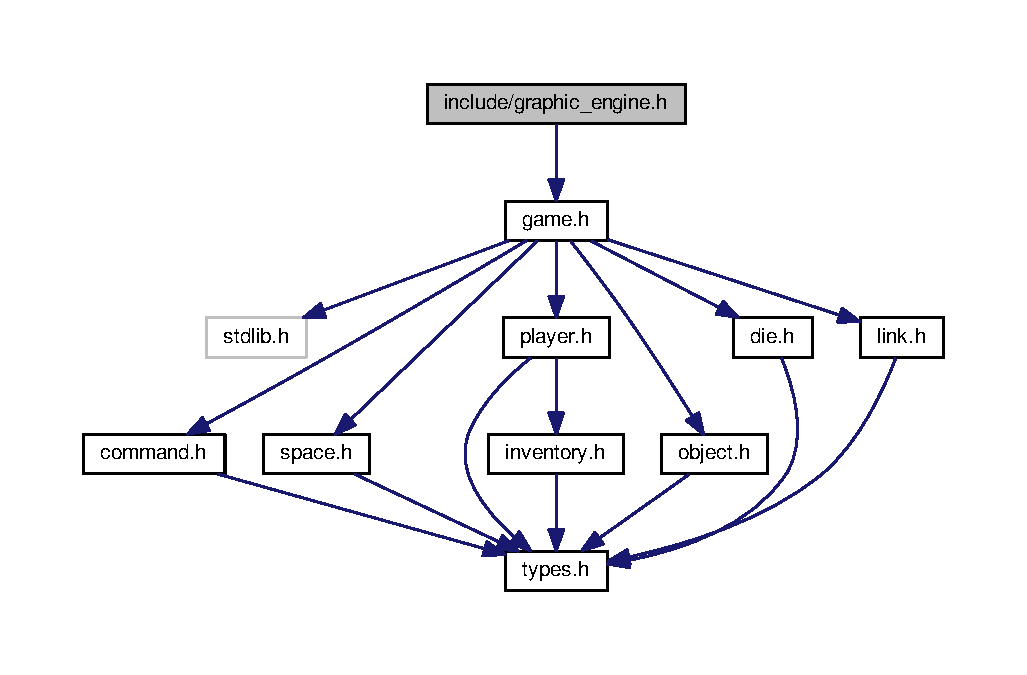
\includegraphics[width=350pt]{graphic__engine_8h__incl}
\end{center}
\end{figure}
\subsection*{Typedefs}
\begin{DoxyCompactItemize}
\item 
typedef struct \+\_\+\+Graphic\+\_\+engine \hyperlink{graphic__engine_8h_ae1bc5cdbfce93098f066274fdea49af1}{Graphic\+\_\+engine}\hypertarget{graphic__engine_8h_ae1bc5cdbfce93098f066274fdea49af1}{}\label{graphic__engine_8h_ae1bc5cdbfce93098f066274fdea49af1}

\begin{DoxyCompactList}\small\item\em It holds the necessary data to manage a Graphic Engine. \end{DoxyCompactList}\end{DoxyCompactItemize}
\subsection*{Functions}
\begin{Indent}{\bf graphic\+\_\+engine\+\_\+create}\par
{\em It allocates memory for a Graphic Engine we will be using to print.

\begin{DoxyAuthor}{Author}
Profesores P\+P\+R\+OG edited by Eric Morales 
\end{DoxyAuthor}
\begin{DoxyVersion}{Version}
2.\+0 
\end{DoxyVersion}
\begin{DoxyDate}{Date}
02-\/03-\/2018 
\end{DoxyDate}
\begin{DoxyReturn}{Returns}
A Graphic Engine. 
\end{DoxyReturn}
}\begin{DoxyCompactItemize}
\item 
\hyperlink{graphic__engine_8h_ae1bc5cdbfce93098f066274fdea49af1}{Graphic\+\_\+engine} $\ast$ {\bfseries graphic\+\_\+engine\+\_\+create} ()\hypertarget{graphic__engine_8h_a8c3d9abe7282bee1d77d23ea80a4bdec}{}\label{graphic__engine_8h_a8c3d9abe7282bee1d77d23ea80a4bdec}

\end{DoxyCompactItemize}
\end{Indent}
\begin{Indent}{\bf graphic\+\_\+engine\+\_\+destroy}\par
{\em It frees the memory a Graphic Engine was allocating.

\begin{DoxyAuthor}{Author}
Profesores P\+P\+R\+OG edited by Eric Morales 
\end{DoxyAuthor}
\begin{DoxyVersion}{Version}
1.\+0 
\end{DoxyVersion}
\begin{DoxyDate}{Date}
02-\/03-\/2018 
\end{DoxyDate}

\begin{DoxyParams}{Parameters}
{\em Graphic\+\_\+engine$\ast$} & -\/$>$ a graphic engine to be freed. \\
\hline
\end{DoxyParams}
\begin{DoxyReturn}{Returns}
A void, with nothing important. 
\end{DoxyReturn}
}\begin{DoxyCompactItemize}
\item 
void {\bfseries graphic\+\_\+engine\+\_\+destroy} (\hyperlink{graphic__engine_8h_ae1bc5cdbfce93098f066274fdea49af1}{Graphic\+\_\+engine} $\ast$ge)\hypertarget{graphic__engine_8h_a5a5eac4ef2033c5ad71aa6895f362f79}{}\label{graphic__engine_8h_a5a5eac4ef2033c5ad71aa6895f362f79}

\end{DoxyCompactItemize}
\end{Indent}
\begin{Indent}{\bf graphic\+\_\+engine\+\_\+paint\+\_\+game}\par
{\em It paints the game on the screen with all its info.

\begin{DoxyAuthor}{Author}
Profesores P\+P\+R\+OG edited by Alejandro Pascual, Eric Morales \& Javier Lougedo. 
\end{DoxyAuthor}
\begin{DoxyVersion}{Version}
3.\+0 
\end{DoxyVersion}
\begin{DoxyDate}{Date}
02-\/03-\/2018 
\end{DoxyDate}

\begin{DoxyParams}{Parameters}
{\em Graphic\+\_\+engine$\ast$} & -\/$>$ a graphic engine that will define where to print. \\
\hline
{\em Game$\ast$} & -\/$>$ a game with the information to print on the screen. \\
\hline
\end{DoxyParams}
\begin{DoxyReturn}{Returns}
A void. 
\end{DoxyReturn}
}\begin{DoxyCompactItemize}
\item 
void {\bfseries graphic\+\_\+engine\+\_\+paint\+\_\+game} (\hyperlink{graphic__engine_8h_ae1bc5cdbfce93098f066274fdea49af1}{Graphic\+\_\+engine} $\ast$ge, \hyperlink{game_8h_a57156d39c530aec3fba3a9dad8c2dc6a}{Game} $\ast$game)\hypertarget{graphic__engine_8h_a0e275aa477d5fa59e903da33a2a40a5d}{}\label{graphic__engine_8h_a0e275aa477d5fa59e903da33a2a40a5d}

\end{DoxyCompactItemize}
\end{Indent}
\begin{Indent}{\bf graphic\+\_\+engine\+\_\+write\+\_\+command}\par
{\em It writes the last command and if it worked on the screen.

\begin{DoxyAuthor}{Author}
Alejandro Pascual. 
\end{DoxyAuthor}
\begin{DoxyVersion}{Version}
3.\+0 
\end{DoxyVersion}
\begin{DoxyDate}{Date}
02-\/03-\/2018 
\end{DoxyDate}

\begin{DoxyParams}{Parameters}
{\em Game$\ast$} & -\/$>$ a game to get the objects from. \\
\hline
{\em Space$\ast$} & -\/$>$ a space where we will \textquotesingle{}extract\textquotesingle{} the objects to print. \\
\hline
\end{DoxyParams}
\begin{DoxyReturn}{Returns}
A char with the symbol of the object (its initial). 
\end{DoxyReturn}
}\begin{DoxyCompactItemize}
\item 
void {\bfseries graphic\+\_\+engine\+\_\+write\+\_\+command} (\hyperlink{graphic__engine_8h_ae1bc5cdbfce93098f066274fdea49af1}{Graphic\+\_\+engine} $\ast$ge, char $\ast$str)\hypertarget{graphic__engine_8h_a112605879db4582a6d9cd6c12bd0e90c}{}\label{graphic__engine_8h_a112605879db4582a6d9cd6c12bd0e90c}

\item 
char $\ast$ {\bfseries graphic\+\_\+engine\+\_\+get\+\_\+objects\+\_\+symbols} (\hyperlink{game_8h_a57156d39c530aec3fba3a9dad8c2dc6a}{Game} $\ast$, \hyperlink{space_8h_a67533ffc2b70463baecc38fb0629bbfc}{Space} $\ast$)\hypertarget{graphic__engine_8h_a6785925a77e9a39e68315b8cee36944f}{}\label{graphic__engine_8h_a6785925a77e9a39e68315b8cee36944f}

\end{DoxyCompactItemize}
\end{Indent}


\subsection{Detailed Description}
It defines a textual graphic engine. 

\begin{DoxyAuthor}{Author}
Profesores P\+P\+R\+OG edited by Javier Lougedo, Victor Yrazusta, Eric Morales \& Alejandro Pascual 
\end{DoxyAuthor}
\begin{DoxyVersion}{Version}
4.\+0 
\end{DoxyVersion}
\begin{DoxyDate}{Date}
18-\/01-\/2017 
\end{DoxyDate}
\begin{DoxyCopyright}{Copyright}
G\+NU Public License 
\end{DoxyCopyright}

\hypertarget{inventory_8h}{}\section{include/inventory.h File Reference}
\label{inventory_8h}\index{include/inventory.\+h@{include/inventory.\+h}}


It implements the inventory interpreter and the different functions needed to use it.  


{\ttfamily \#include \char`\"{}types.\+h\char`\"{}}\\*
Include dependency graph for inventory.\+h\+:\nopagebreak
\begin{figure}[H]
\begin{center}
\leavevmode
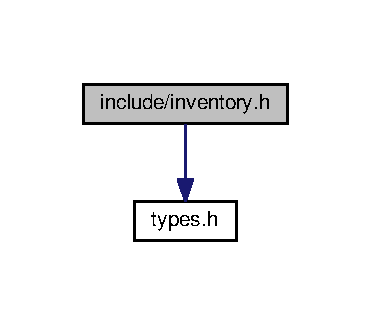
\includegraphics[width=178pt]{inventory_8h__incl}
\end{center}
\end{figure}
This graph shows which files directly or indirectly include this file\+:\nopagebreak
\begin{figure}[H]
\begin{center}
\leavevmode
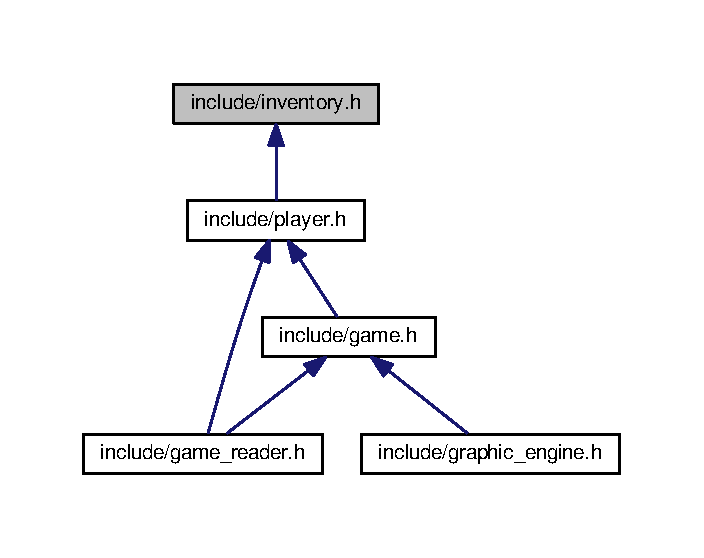
\includegraphics[width=338pt]{inventory_8h__dep__incl}
\end{center}
\end{figure}
\subsection*{Typedefs}
\begin{DoxyCompactItemize}
\item 
typedef struct \+\_\+\+Inventory \hyperlink{inventory_8h_a2253bf64ac4ce6a9c1d6f39c0b0d32a3}{Inventory}\hypertarget{inventory_8h_a2253bf64ac4ce6a9c1d6f39c0b0d32a3}{}\label{inventory_8h_a2253bf64ac4ce6a9c1d6f39c0b0d32a3}

\begin{DoxyCompactList}\small\item\em It holds the necessary data to manage an inventory. \end{DoxyCompactList}\end{DoxyCompactItemize}
\subsection*{Functions}
\begin{Indent}{\bf inventory\+\_\+create}\par
{\em It creates an Inventory with the passed int as its capacity.

\begin{DoxyAuthor}{Author}
Alejandro Pascual 
\end{DoxyAuthor}
\begin{DoxyVersion}{Version}
1.\+0 
\end{DoxyVersion}
\begin{DoxyDate}{Date}
01-\/04-\/2018 
\end{DoxyDate}

\begin{DoxyParams}{Parameters}
{\em int} & -\/$>$ an integer with the capacity of the new inventory. \\
\hline
\end{DoxyParams}
\begin{DoxyReturn}{Returns}
An Inventory$\ast$, which points towards the created inventory. 
\end{DoxyReturn}
}\begin{DoxyCompactItemize}
\item 
\hyperlink{inventory_8h_a2253bf64ac4ce6a9c1d6f39c0b0d32a3}{Inventory} $\ast$ {\bfseries inventory\+\_\+create} (int max\+\_\+ids)\hypertarget{inventory_8h_abcf6f24e277f673a39437523a1e4a286}{}\label{inventory_8h_abcf6f24e277f673a39437523a1e4a286}

\end{DoxyCompactItemize}
\end{Indent}
\begin{Indent}{\bf inventory\+\_\+destroy}\par
{\em It destroys the Inventory passed.

\begin{DoxyAuthor}{Author}
Alejandro Pascual 
\end{DoxyAuthor}
\begin{DoxyVersion}{Version}
1.\+0 
\end{DoxyVersion}
\begin{DoxyDate}{Date}
01-\/04-\/2018 
\end{DoxyDate}

\begin{DoxyParams}{Parameters}
{\em Inventory$\ast$} & -\/$>$ the inventory we are willing to destroy. \\
\hline
\end{DoxyParams}
\begin{DoxyReturn}{Returns}
A S\+T\+A\+T\+US, which indicates whether the operation could be executed correctly. 
\end{DoxyReturn}
}\begin{DoxyCompactItemize}
\item 
\hyperlink{types_8h_a32c27cc471df37f4fc818d65de0a56c4}{S\+T\+A\+T\+US} {\bfseries inventory\+\_\+destroy} (\hyperlink{inventory_8h_a2253bf64ac4ce6a9c1d6f39c0b0d32a3}{Inventory} $\ast$)\hypertarget{inventory_8h_a5d82d8e66a459a366d26d70f312504f5}{}\label{inventory_8h_a5d82d8e66a459a366d26d70f312504f5}

\end{DoxyCompactItemize}
\end{Indent}
\begin{Indent}{\bf inventory\+\_\+add}\par
{\em It adds the passed Id to the Set of the Inventory.

\begin{DoxyAuthor}{Author}
Alejandro Pascual 
\end{DoxyAuthor}
\begin{DoxyVersion}{Version}
1.\+0 
\end{DoxyVersion}
\begin{DoxyDate}{Date}
01-\/04-\/2018 
\end{DoxyDate}

\begin{DoxyParams}{Parameters}
{\em Inventory$\ast$} & -\/$>$ the inventory we are willing to add an (object) id in. \\
\hline
{\em Id} & -\/$>$ the Id of the object (or other). \\
\hline
\end{DoxyParams}
\begin{DoxyReturn}{Returns}
A S\+T\+A\+T\+US, which indicates whether the operation could be executed correctly. 
\end{DoxyReturn}
}\begin{DoxyCompactItemize}
\item 
\hyperlink{types_8h_a32c27cc471df37f4fc818d65de0a56c4}{S\+T\+A\+T\+US} {\bfseries inventory\+\_\+add} (\hyperlink{inventory_8h_a2253bf64ac4ce6a9c1d6f39c0b0d32a3}{Inventory} $\ast$, \hyperlink{types_8h_a845e604fb28f7e3d97549da3448149d3}{Id} object\+\_\+id)\hypertarget{inventory_8h_a9ad6d908b5f9c83b251b19d7286aef28}{}\label{inventory_8h_a9ad6d908b5f9c83b251b19d7286aef28}

\end{DoxyCompactItemize}
\end{Indent}
\begin{Indent}{\bf inventory\+\_\+del}\par
{\em It removes the passed Id from the Set of the Inventory.

\begin{DoxyAuthor}{Author}
Alejandro Pascual 
\end{DoxyAuthor}
\begin{DoxyVersion}{Version}
1.\+0 
\end{DoxyVersion}
\begin{DoxyDate}{Date}
01-\/04-\/2018 
\end{DoxyDate}

\begin{DoxyParams}{Parameters}
{\em Inventory$\ast$} & -\/$>$ the inventory we want to delete an object in. \\
\hline
{\em Id} & -\/$>$ the Id of the object to be destroyed of the inventory. \\
\hline
\end{DoxyParams}
\begin{DoxyReturn}{Returns}
A S\+T\+A\+T\+US, which indicates whether the operation could be executed correctly. 
\end{DoxyReturn}
}\begin{DoxyCompactItemize}
\item 
\hyperlink{types_8h_a32c27cc471df37f4fc818d65de0a56c4}{S\+T\+A\+T\+US} {\bfseries inventory\+\_\+del} (\hyperlink{inventory_8h_a2253bf64ac4ce6a9c1d6f39c0b0d32a3}{Inventory} $\ast$, \hyperlink{types_8h_a845e604fb28f7e3d97549da3448149d3}{Id} object\+\_\+id)\hypertarget{inventory_8h_a031c411e1e061161da757efef99a82b8}{}\label{inventory_8h_a031c411e1e061161da757efef99a82b8}

\end{DoxyCompactItemize}
\end{Indent}
\begin{Indent}{\bf inventory\+\_\+set\+\_\+max\+\_\+objects}\par
{\em It sets the capacity of the Inventory.

\begin{DoxyAuthor}{Author}
Alejandro Pascual 
\end{DoxyAuthor}
\begin{DoxyVersion}{Version}
1.\+0 
\end{DoxyVersion}
\begin{DoxyDate}{Date}
01-\/04-\/2018 
\end{DoxyDate}

\begin{DoxyParams}{Parameters}
{\em Inventory$\ast$} & -\/$>$ the inventory whose max\+\_\+objects is going to be set. \\
\hline
{\em int} & -\/$>$ an integer that will define the capacity of the Inventory. \\
\hline
\end{DoxyParams}
\begin{DoxyReturn}{Returns}
A S\+T\+A\+T\+US, which indicates whether the operation could be executed correctly. 
\end{DoxyReturn}
}\begin{DoxyCompactItemize}
\item 
\hyperlink{types_8h_a32c27cc471df37f4fc818d65de0a56c4}{S\+T\+A\+T\+US} {\bfseries inventory\+\_\+set\+\_\+max\+\_\+objects} (\hyperlink{inventory_8h_a2253bf64ac4ce6a9c1d6f39c0b0d32a3}{Inventory} $\ast$, int max\+\_\+objects)\hypertarget{inventory_8h_ac8f4bb3a7415d3b6d887a93680e64949}{}\label{inventory_8h_ac8f4bb3a7415d3b6d887a93680e64949}

\end{DoxyCompactItemize}
\end{Indent}
\begin{Indent}{\bf inventory\+\_\+get\+\_\+object\+\_\+id}\par
{\em It returns the Id of the specified position in the Set of the Inventory.

\begin{DoxyAuthor}{Author}
Alejandro Pascual 
\end{DoxyAuthor}
\begin{DoxyVersion}{Version}
1.\+0 
\end{DoxyVersion}
\begin{DoxyDate}{Date}
01-\/04-\/2018 
\end{DoxyDate}

\begin{DoxyParams}{Parameters}
{\em Inventory$\ast$} & -\/$>$ the inventory we are going to get the object from. \\
\hline
{\em int} & -\/$>$ an integer that will specifie the position of the Id in the Set of the Inventory. \\
\hline
\end{DoxyParams}
\begin{DoxyReturn}{Returns}
The Id of the specified position in the Set of the Inventory. 
\end{DoxyReturn}
}\begin{DoxyCompactItemize}
\item 
\hyperlink{types_8h_a845e604fb28f7e3d97549da3448149d3}{Id} {\bfseries inventory\+\_\+get\+\_\+object\+\_\+id} (\hyperlink{inventory_8h_a2253bf64ac4ce6a9c1d6f39c0b0d32a3}{Inventory} $\ast$, int position)\hypertarget{inventory_8h_aaf1dddaa358d892a07aacc12c681db21}{}\label{inventory_8h_aaf1dddaa358d892a07aacc12c681db21}

\end{DoxyCompactItemize}
\end{Indent}
\begin{Indent}{\bf inventory\+\_\+get\+\_\+objects\+\_\+number}\par
{\em It returns the current number of Ids in Set of the Inventory.

\begin{DoxyAuthor}{Author}
Alejandro Pascual 
\end{DoxyAuthor}
\begin{DoxyVersion}{Version}
1.\+0 
\end{DoxyVersion}
\begin{DoxyDate}{Date}
01-\/04-\/2018 
\end{DoxyDate}

\begin{DoxyParams}{Parameters}
{\em Inventory$\ast$} & -\/$>$ the inventory we want to get the quantity of objects in. \\
\hline
\end{DoxyParams}
\begin{DoxyReturn}{Returns}
The current number of Ids in Set of the Inventory. 
\end{DoxyReturn}
}\begin{DoxyCompactItemize}
\item 
int {\bfseries inventory\+\_\+get\+\_\+objects\+\_\+number} (\hyperlink{inventory_8h_a2253bf64ac4ce6a9c1d6f39c0b0d32a3}{Inventory} $\ast$)\hypertarget{inventory_8h_a7c3c1ed9aa24751075f36cdb37a42db6}{}\label{inventory_8h_a7c3c1ed9aa24751075f36cdb37a42db6}

\end{DoxyCompactItemize}
\end{Indent}
\begin{Indent}{\bf inventory\+\_\+get\+\_\+max\+\_\+objects}\par
{\em It returns the capacity of the Inventory.

\begin{DoxyAuthor}{Author}
Alejandro Pascual 
\end{DoxyAuthor}
\begin{DoxyVersion}{Version}
1.\+0 
\end{DoxyVersion}
\begin{DoxyDate}{Date}
01-\/04-\/2018 
\end{DoxyDate}

\begin{DoxyParams}{Parameters}
{\em Inventory$\ast$} & -\/$>$ the Inventory we want to get the max objects from. \\
\hline
\end{DoxyParams}
\begin{DoxyReturn}{Returns}
The capacity of the inventory as an int. 
\end{DoxyReturn}
}\begin{DoxyCompactItemize}
\item 
int {\bfseries inventory\+\_\+get\+\_\+max\+\_\+objects} (\hyperlink{inventory_8h_a2253bf64ac4ce6a9c1d6f39c0b0d32a3}{Inventory} $\ast$)\hypertarget{inventory_8h_a2938d0f22f713aa19214169708811356}{}\label{inventory_8h_a2938d0f22f713aa19214169708811356}

\end{DoxyCompactItemize}
\end{Indent}
\begin{Indent}{\bf inventory\+\_\+check\+\_\+object}\par
{\em It checks if the passed Id is on the Set of the Inventory.

\begin{DoxyAuthor}{Author}
Alejandro Pascual 
\end{DoxyAuthor}
\begin{DoxyVersion}{Version}
1.\+0 
\end{DoxyVersion}
\begin{DoxyDate}{Date}
01-\/04-\/2018 
\end{DoxyDate}

\begin{DoxyParams}{Parameters}
{\em Inventory$\ast$} & -\/$>$ the inventory we are going to check in. \\
\hline
{\em Id} & -\/$>$ the Id of the object to be checked. \\
\hline
\end{DoxyParams}
\begin{DoxyReturn}{Returns}
A B\+O\+OL, which is T\+R\+UE if the object is in the Set. 
\end{DoxyReturn}
}\begin{DoxyCompactItemize}
\item 
\hyperlink{types_8h_a3e5b8192e7d9ffaf3542f1210aec18dd}{B\+O\+OL} {\bfseries inventory\+\_\+check\+\_\+object} (\hyperlink{inventory_8h_a2253bf64ac4ce6a9c1d6f39c0b0d32a3}{Inventory} $\ast$, \hyperlink{types_8h_a845e604fb28f7e3d97549da3448149d3}{Id} object\+\_\+id)\hypertarget{inventory_8h_ad5a6495fb65ec1fa4a3a076e15a7e3e8}{}\label{inventory_8h_ad5a6495fb65ec1fa4a3a076e15a7e3e8}

\end{DoxyCompactItemize}
\end{Indent}
\begin{Indent}{\bf inventory\+\_\+is\+\_\+empty}\par
{\em It checks if the Set of the Inventory is empty.

\begin{DoxyAuthor}{Author}
Alejandro Pascual 
\end{DoxyAuthor}
\begin{DoxyVersion}{Version}
1.\+0 
\end{DoxyVersion}
\begin{DoxyDate}{Date}
01-\/04-\/2018 
\end{DoxyDate}

\begin{DoxyParams}{Parameters}
{\em Inventory$\ast$} & -\/$>$ the inventory we will check if empty or not. \\
\hline
\end{DoxyParams}
\begin{DoxyReturn}{Returns}
A B\+O\+OL, which is T\+R\+UE if the Set of the Inventory is empty or if the Inventory$\ast$ is N\+U\+LL. 
\end{DoxyReturn}
}\begin{DoxyCompactItemize}
\item 
\hyperlink{types_8h_a3e5b8192e7d9ffaf3542f1210aec18dd}{B\+O\+OL} {\bfseries inventory\+\_\+is\+\_\+empty} (\hyperlink{inventory_8h_a2253bf64ac4ce6a9c1d6f39c0b0d32a3}{Inventory} $\ast$)\hypertarget{inventory_8h_a4789367383af94d5f789a6fc544675a5}{}\label{inventory_8h_a4789367383af94d5f789a6fc544675a5}

\end{DoxyCompactItemize}
\end{Indent}
\begin{Indent}{\bf inventory\+\_\+is\+\_\+full}\par
{\em It checks if the Set of the Inventory is full.

\begin{DoxyAuthor}{Author}
Alejandro Pascual 
\end{DoxyAuthor}
\begin{DoxyVersion}{Version}
1.\+0 
\end{DoxyVersion}
\begin{DoxyDate}{Date}
01-\/04-\/2018 
\end{DoxyDate}

\begin{DoxyParams}{Parameters}
{\em Inventory$\ast$} & -\/$>$ the inventory we will check if full or not. \\
\hline
\end{DoxyParams}
\begin{DoxyReturn}{Returns}
A B\+O\+OL, which is T\+R\+UE if the Set of the Inventory is full or if the Inventory$\ast$ is N\+U\+LL. 
\end{DoxyReturn}
}\begin{DoxyCompactItemize}
\item 
\hyperlink{types_8h_a3e5b8192e7d9ffaf3542f1210aec18dd}{B\+O\+OL} {\bfseries inventory\+\_\+is\+\_\+full} (\hyperlink{inventory_8h_a2253bf64ac4ce6a9c1d6f39c0b0d32a3}{Inventory} $\ast$)\hypertarget{inventory_8h_adeab3119b7030970980db8d25f60d3bd}{}\label{inventory_8h_adeab3119b7030970980db8d25f60d3bd}

\end{DoxyCompactItemize}
\end{Indent}
\begin{Indent}{\bf inventory\+\_\+print}\par
{\em It prints the content of the Set of the Inventory.

\begin{DoxyAuthor}{Author}
Alejandro Pascual 
\end{DoxyAuthor}
\begin{DoxyVersion}{Version}
1.\+0 
\end{DoxyVersion}
\begin{DoxyDate}{Date}
01-\/04-\/2018 
\end{DoxyDate}

\begin{DoxyParams}{Parameters}
{\em Inventory$\ast$} & -\/$>$ the inventory to be printed. \\
\hline
\end{DoxyParams}
\begin{DoxyReturn}{Returns}
A S\+T\+A\+T\+US, which indicates whether the operation could be executed correctly.
\end{DoxyReturn}
N\+O\+TE\+: This function was created for debugging purposes only and it is not used in the normal execution of the game. }\begin{DoxyCompactItemize}
\item 
\hyperlink{types_8h_a32c27cc471df37f4fc818d65de0a56c4}{S\+T\+A\+T\+US} {\bfseries inventory\+\_\+print} (\hyperlink{inventory_8h_a2253bf64ac4ce6a9c1d6f39c0b0d32a3}{Inventory} $\ast$)\hypertarget{inventory_8h_aa91cd1c1be9d1cbdfb72d2b48346d4fd}{}\label{inventory_8h_aa91cd1c1be9d1cbdfb72d2b48346d4fd}

\end{DoxyCompactItemize}
\end{Indent}


\subsection{Detailed Description}
It implements the inventory interpreter and the different functions needed to use it. 

\begin{DoxyAuthor}{Author}
Alejandro Pascual. 
\end{DoxyAuthor}
\begin{DoxyVersion}{Version}
1.\+0 
\end{DoxyVersion}
\begin{DoxyDate}{Date}
01-\/04-\/2018 (creation) 
\end{DoxyDate}
\begin{DoxyCopyright}{Copyright}
G\+NU Public License 
\end{DoxyCopyright}

\hypertarget{inventory__test_8h}{}\section{include/inventory\+\_\+test.h File Reference}
\label{inventory__test_8h}\index{include/inventory\+\_\+test.\+h@{include/inventory\+\_\+test.\+h}}


It declares the tests for the Inventory module.  


\subsection*{Functions}
\begin{DoxyCompactItemize}
\item 
void \hyperlink{inventory__test_8h_a33638f1a88ae16ab8d6bee00145b82b8}{test1\+\_\+inventory\+\_\+create} ()
\item 
void \hyperlink{inventory__test_8h_a73a6080c360a8870c4ffc734e989c8b3}{test2\+\_\+inventory\+\_\+create} ()
\item 
void \hyperlink{inventory__test_8h_ab161eafe6a61db39b2237e97c677d822}{test1\+\_\+inventory\+\_\+destroy} ()
\item 
void \hyperlink{inventory__test_8h_a9f3daec28c696c0671e6a3e905359741}{test2\+\_\+inventory\+\_\+destroy} ()
\item 
void \hyperlink{inventory__test_8h_ae81ec4669af03331ca8a228567736474}{test1\+\_\+inventory\+\_\+add} ()
\item 
void \hyperlink{inventory__test_8h_a48019cb45cb5918233d5d42334d2be17}{test2\+\_\+inventory\+\_\+add} ()
\item 
void \hyperlink{inventory__test_8h_ada5ad194dfe9af537c6b2805bf38910d}{test3\+\_\+inventory\+\_\+add} ()
\item 
void \hyperlink{inventory__test_8h_afe091fc610e1df3c1d0982754ea1ae7f}{test4\+\_\+inventory\+\_\+add} ()
\item 
void \hyperlink{inventory__test_8h_a0198822eb71da7d7e1a8742e6953c82c}{test1\+\_\+inventory\+\_\+del} ()
\item 
void \hyperlink{inventory__test_8h_a242baf98676c3685d4696ec6c006cbb9}{test2\+\_\+inventory\+\_\+del} ()
\item 
void \hyperlink{inventory__test_8h_a063d13c3dbc32094f20fe98ca0c6c357}{test3\+\_\+inventory\+\_\+del} ()
\item 
void \hyperlink{inventory__test_8h_a8df246f77e3ca2cdaf6162bd88eda9ef}{test4\+\_\+inventory\+\_\+del} ()
\item 
void \hyperlink{inventory__test_8h_aedc895d6409678b2176d822c105c3796}{test1\+\_\+inventory\+\_\+set\+\_\+max\+\_\+objects} ()
\item 
void \hyperlink{inventory__test_8h_aff93a7fb7ffbac1890ce563012a9d372}{test2\+\_\+inventory\+\_\+set\+\_\+max\+\_\+objects} ()
\item 
void \hyperlink{inventory__test_8h_a270c2d6aecda0d73fbcff6ca0c9a90db}{test3\+\_\+inventory\+\_\+set\+\_\+max\+\_\+objects} ()
\item 
void \hyperlink{inventory__test_8h_ad7af47985db2fe8d44d715df81414f33}{test4\+\_\+inventory\+\_\+set\+\_\+max\+\_\+objects} ()
\item 
void \hyperlink{inventory__test_8h_a7feab32c68817ece1716946f02738dc5}{test1\+\_\+inventory\+\_\+get\+\_\+object\+\_\+id} ()
\item 
void \hyperlink{inventory__test_8h_a41ba2562e1c60e222110f05c9a8e221e}{test2\+\_\+inventory\+\_\+get\+\_\+object\+\_\+id} ()
\item 
void \hyperlink{inventory__test_8h_af4188f35f25167e033fab87480f69c72}{test3\+\_\+inventory\+\_\+get\+\_\+object\+\_\+id} ()
\item 
void \hyperlink{inventory__test_8h_a03ef2e867bad9b096df6047fcb22331e}{test1\+\_\+inventory\+\_\+get\+\_\+objects\+\_\+number} ()
\item 
void \hyperlink{inventory__test_8h_a3546785f0cda504b4d16c89c19f0b23e}{test2\+\_\+inventory\+\_\+get\+\_\+objects\+\_\+number} ()
\item 
void \hyperlink{inventory__test_8h_adc6cd2ad429ac85285e5f40619c2e06b}{test3\+\_\+inventory\+\_\+get\+\_\+objects\+\_\+number} ()
\item 
void \hyperlink{inventory__test_8h_a17c5d7d6ecb4161696deca0155e13f4f}{test1\+\_\+inventory\+\_\+get\+\_\+max\+\_\+objects} ()
\item 
void \hyperlink{inventory__test_8h_ac75954611acab583f780145532ab3197}{test2\+\_\+inventory\+\_\+get\+\_\+max\+\_\+objects} ()
\item 
void \hyperlink{inventory__test_8h_aee11f25fc989fa8d62b5115f30b48edc}{test3\+\_\+inventory\+\_\+get\+\_\+max\+\_\+objects} ()
\item 
void \hyperlink{inventory__test_8h_a94926e4449b777046515a173637bee84}{test1\+\_\+inventory\+\_\+check\+\_\+object} ()
\item 
void \hyperlink{inventory__test_8h_a847aa346d12ebb77d86d202bd0fa99b6}{test2\+\_\+inventory\+\_\+check\+\_\+object} ()
\item 
void \hyperlink{inventory__test_8h_a4f88e37d67c69f990b82b135f5c1f9f9}{test3\+\_\+inventory\+\_\+check\+\_\+object} ()
\item 
void \hyperlink{inventory__test_8h_afe8c9730e30b58535afc0481970ab2b1}{test1\+\_\+inventory\+\_\+is\+\_\+empty} ()
\item 
void \hyperlink{inventory__test_8h_a4d2a2a4d4ba59446d013debfe9bf05dc}{test2\+\_\+inventory\+\_\+is\+\_\+empty} ()
\item 
void \hyperlink{inventory__test_8h_a9c8daeb141dbec6ddd5621edade53091}{test3\+\_\+inventory\+\_\+is\+\_\+empty} ()
\item 
void \hyperlink{inventory__test_8h_a7eb3ba387e33c42ff45331c9d9aada34}{test1\+\_\+inventory\+\_\+is\+\_\+full} ()
\item 
void \hyperlink{inventory__test_8h_a1c9e567d4919d5aaccc9580815a8a81d}{test2\+\_\+inventory\+\_\+is\+\_\+full} ()
\item 
void \hyperlink{inventory__test_8h_a540dbcbfd29bd63590d081e496f8227f}{test3\+\_\+inventory\+\_\+is\+\_\+full} ()
\end{DoxyCompactItemize}


\subsection{Detailed Description}
It declares the tests for the Inventory module. 

\begin{DoxyAuthor}{Author}
Alejandro Pascual 
\end{DoxyAuthor}
\begin{DoxyVersion}{Version}
1.\+0 
\end{DoxyVersion}
\begin{DoxyDate}{Date}
06-\/04-\/2018 (creation) 
\end{DoxyDate}
\begin{DoxyCopyright}{Copyright}
G\+NU Public License 
\end{DoxyCopyright}


\subsection{Function Documentation}
\index{inventory\+\_\+test.\+h@{inventory\+\_\+test.\+h}!test1\+\_\+inventory\+\_\+add@{test1\+\_\+inventory\+\_\+add}}
\index{test1\+\_\+inventory\+\_\+add@{test1\+\_\+inventory\+\_\+add}!inventory\+\_\+test.\+h@{inventory\+\_\+test.\+h}}
\subsubsection[{\texorpdfstring{test1\+\_\+inventory\+\_\+add()}{test1_inventory_add()}}]{\setlength{\rightskip}{0pt plus 5cm}void test1\+\_\+inventory\+\_\+add (
\begin{DoxyParamCaption}
{}
\end{DoxyParamCaption}
)}\hypertarget{inventory__test_8h_ae81ec4669af03331ca8a228567736474}{}\label{inventory__test_8h_ae81ec4669af03331ca8a228567736474}
\begin{DoxyRefDesc}{Test}
\item[\hyperlink{test__test000093}{Test}]Test function for adding an object \end{DoxyRefDesc}
\begin{DoxyPrecond}{Precondition}
A non full Inventory and a valid Id 
\end{DoxyPrecond}
\begin{DoxyPostcond}{Postcondition}
OK. The inventory must contain the passed Id 
\end{DoxyPostcond}
\index{inventory\+\_\+test.\+h@{inventory\+\_\+test.\+h}!test1\+\_\+inventory\+\_\+check\+\_\+object@{test1\+\_\+inventory\+\_\+check\+\_\+object}}
\index{test1\+\_\+inventory\+\_\+check\+\_\+object@{test1\+\_\+inventory\+\_\+check\+\_\+object}!inventory\+\_\+test.\+h@{inventory\+\_\+test.\+h}}
\subsubsection[{\texorpdfstring{test1\+\_\+inventory\+\_\+check\+\_\+object()}{test1_inventory_check_object()}}]{\setlength{\rightskip}{0pt plus 5cm}void test1\+\_\+inventory\+\_\+check\+\_\+object (
\begin{DoxyParamCaption}
{}
\end{DoxyParamCaption}
)}\hypertarget{inventory__test_8h_a94926e4449b777046515a173637bee84}{}\label{inventory__test_8h_a94926e4449b777046515a173637bee84}
\begin{DoxyRefDesc}{Test}
\item[\hyperlink{test__test000114}{Test}]Test function for checking if an Object Id is in the Inventory \end{DoxyRefDesc}
\begin{DoxyPrecond}{Precondition}
An Inventory with an Id and that Id 
\end{DoxyPrecond}
\begin{DoxyPostcond}{Postcondition}
T\+R\+UE 
\end{DoxyPostcond}
\index{inventory\+\_\+test.\+h@{inventory\+\_\+test.\+h}!test1\+\_\+inventory\+\_\+create@{test1\+\_\+inventory\+\_\+create}}
\index{test1\+\_\+inventory\+\_\+create@{test1\+\_\+inventory\+\_\+create}!inventory\+\_\+test.\+h@{inventory\+\_\+test.\+h}}
\subsubsection[{\texorpdfstring{test1\+\_\+inventory\+\_\+create()}{test1_inventory_create()}}]{\setlength{\rightskip}{0pt plus 5cm}void test1\+\_\+inventory\+\_\+create (
\begin{DoxyParamCaption}
{}
\end{DoxyParamCaption}
)}\hypertarget{inventory__test_8h_a33638f1a88ae16ab8d6bee00145b82b8}{}\label{inventory__test_8h_a33638f1a88ae16ab8d6bee00145b82b8}
\begin{DoxyRefDesc}{Test}
\item[\hyperlink{test__test000089}{Test}]Test function for inventory creation \end{DoxyRefDesc}
\begin{DoxyPrecond}{Precondition}
A capacity of 0 or more 
\end{DoxyPrecond}
\begin{DoxyPostcond}{Postcondition}
Non N\+U\+LL pointer to Inventory with the passed capacity 
\end{DoxyPostcond}
\index{inventory\+\_\+test.\+h@{inventory\+\_\+test.\+h}!test1\+\_\+inventory\+\_\+del@{test1\+\_\+inventory\+\_\+del}}
\index{test1\+\_\+inventory\+\_\+del@{test1\+\_\+inventory\+\_\+del}!inventory\+\_\+test.\+h@{inventory\+\_\+test.\+h}}
\subsubsection[{\texorpdfstring{test1\+\_\+inventory\+\_\+del()}{test1_inventory_del()}}]{\setlength{\rightskip}{0pt plus 5cm}void test1\+\_\+inventory\+\_\+del (
\begin{DoxyParamCaption}
{}
\end{DoxyParamCaption}
)}\hypertarget{inventory__test_8h_a0198822eb71da7d7e1a8742e6953c82c}{}\label{inventory__test_8h_a0198822eb71da7d7e1a8742e6953c82c}
\begin{DoxyRefDesc}{Test}
\item[\hyperlink{test__test000097}{Test}]Test function for deleting an object \end{DoxyRefDesc}
\begin{DoxyPrecond}{Precondition}
An Inventory with an Id and that Id 
\end{DoxyPrecond}
\begin{DoxyPostcond}{Postcondition}
OK. The inventory mustn\textquotesingle{}t contain the passed Id. 
\end{DoxyPostcond}
\index{inventory\+\_\+test.\+h@{inventory\+\_\+test.\+h}!test1\+\_\+inventory\+\_\+destroy@{test1\+\_\+inventory\+\_\+destroy}}
\index{test1\+\_\+inventory\+\_\+destroy@{test1\+\_\+inventory\+\_\+destroy}!inventory\+\_\+test.\+h@{inventory\+\_\+test.\+h}}
\subsubsection[{\texorpdfstring{test1\+\_\+inventory\+\_\+destroy()}{test1_inventory_destroy()}}]{\setlength{\rightskip}{0pt plus 5cm}void test1\+\_\+inventory\+\_\+destroy (
\begin{DoxyParamCaption}
{}
\end{DoxyParamCaption}
)}\hypertarget{inventory__test_8h_ab161eafe6a61db39b2237e97c677d822}{}\label{inventory__test_8h_ab161eafe6a61db39b2237e97c677d822}
\begin{DoxyRefDesc}{Test}
\item[\hyperlink{test__test000091}{Test}]Test function for inventory destruction \end{DoxyRefDesc}
\begin{DoxyPrecond}{Precondition}
A non N\+U\+LL Inventory pointer 
\end{DoxyPrecond}
\begin{DoxyPostcond}{Postcondition}
OK 
\end{DoxyPostcond}
\index{inventory\+\_\+test.\+h@{inventory\+\_\+test.\+h}!test1\+\_\+inventory\+\_\+get\+\_\+max\+\_\+objects@{test1\+\_\+inventory\+\_\+get\+\_\+max\+\_\+objects}}
\index{test1\+\_\+inventory\+\_\+get\+\_\+max\+\_\+objects@{test1\+\_\+inventory\+\_\+get\+\_\+max\+\_\+objects}!inventory\+\_\+test.\+h@{inventory\+\_\+test.\+h}}
\subsubsection[{\texorpdfstring{test1\+\_\+inventory\+\_\+get\+\_\+max\+\_\+objects()}{test1_inventory_get_max_objects()}}]{\setlength{\rightskip}{0pt plus 5cm}void test1\+\_\+inventory\+\_\+get\+\_\+max\+\_\+objects (
\begin{DoxyParamCaption}
{}
\end{DoxyParamCaption}
)}\hypertarget{inventory__test_8h_a17c5d7d6ecb4161696deca0155e13f4f}{}\label{inventory__test_8h_a17c5d7d6ecb4161696deca0155e13f4f}
\begin{DoxyRefDesc}{Test}
\item[\hyperlink{test__test000111}{Test}]Test function for getting the capacity \end{DoxyRefDesc}
\begin{DoxyPrecond}{Precondition}
An Inventory with a capacity of more than 0 
\end{DoxyPrecond}
\begin{DoxyPostcond}{Postcondition}
A capacity of more than 0 
\end{DoxyPostcond}
\index{inventory\+\_\+test.\+h@{inventory\+\_\+test.\+h}!test1\+\_\+inventory\+\_\+get\+\_\+object\+\_\+id@{test1\+\_\+inventory\+\_\+get\+\_\+object\+\_\+id}}
\index{test1\+\_\+inventory\+\_\+get\+\_\+object\+\_\+id@{test1\+\_\+inventory\+\_\+get\+\_\+object\+\_\+id}!inventory\+\_\+test.\+h@{inventory\+\_\+test.\+h}}
\subsubsection[{\texorpdfstring{test1\+\_\+inventory\+\_\+get\+\_\+object\+\_\+id()}{test1_inventory_get_object_id()}}]{\setlength{\rightskip}{0pt plus 5cm}void test1\+\_\+inventory\+\_\+get\+\_\+object\+\_\+id (
\begin{DoxyParamCaption}
{}
\end{DoxyParamCaption}
)}\hypertarget{inventory__test_8h_a7feab32c68817ece1716946f02738dc5}{}\label{inventory__test_8h_a7feab32c68817ece1716946f02738dc5}
\begin{DoxyRefDesc}{Test}
\item[\hyperlink{test__test000105}{Test}]Test function for getting an Object Id \end{DoxyRefDesc}
\begin{DoxyPrecond}{Precondition}
A non empty Inventory and a position with an Id 
\end{DoxyPrecond}
\begin{DoxyPostcond}{Postcondition}
The Id in the specified position. 
\end{DoxyPostcond}
\index{inventory\+\_\+test.\+h@{inventory\+\_\+test.\+h}!test1\+\_\+inventory\+\_\+get\+\_\+objects\+\_\+number@{test1\+\_\+inventory\+\_\+get\+\_\+objects\+\_\+number}}
\index{test1\+\_\+inventory\+\_\+get\+\_\+objects\+\_\+number@{test1\+\_\+inventory\+\_\+get\+\_\+objects\+\_\+number}!inventory\+\_\+test.\+h@{inventory\+\_\+test.\+h}}
\subsubsection[{\texorpdfstring{test1\+\_\+inventory\+\_\+get\+\_\+objects\+\_\+number()}{test1_inventory_get_objects_number()}}]{\setlength{\rightskip}{0pt plus 5cm}void test1\+\_\+inventory\+\_\+get\+\_\+objects\+\_\+number (
\begin{DoxyParamCaption}
{}
\end{DoxyParamCaption}
)}\hypertarget{inventory__test_8h_a03ef2e867bad9b096df6047fcb22331e}{}\label{inventory__test_8h_a03ef2e867bad9b096df6047fcb22331e}
\begin{DoxyRefDesc}{Test}
\item[\hyperlink{test__test000108}{Test}]Test function for getting the current number of Objects Ids \end{DoxyRefDesc}
\begin{DoxyPrecond}{Precondition}
A non empty Inventory 
\end{DoxyPrecond}
\begin{DoxyPostcond}{Postcondition}
A value of more than 0 
\end{DoxyPostcond}
\index{inventory\+\_\+test.\+h@{inventory\+\_\+test.\+h}!test1\+\_\+inventory\+\_\+is\+\_\+empty@{test1\+\_\+inventory\+\_\+is\+\_\+empty}}
\index{test1\+\_\+inventory\+\_\+is\+\_\+empty@{test1\+\_\+inventory\+\_\+is\+\_\+empty}!inventory\+\_\+test.\+h@{inventory\+\_\+test.\+h}}
\subsubsection[{\texorpdfstring{test1\+\_\+inventory\+\_\+is\+\_\+empty()}{test1_inventory_is_empty()}}]{\setlength{\rightskip}{0pt plus 5cm}void test1\+\_\+inventory\+\_\+is\+\_\+empty (
\begin{DoxyParamCaption}
{}
\end{DoxyParamCaption}
)}\hypertarget{inventory__test_8h_afe8c9730e30b58535afc0481970ab2b1}{}\label{inventory__test_8h_afe8c9730e30b58535afc0481970ab2b1}
\begin{DoxyRefDesc}{Test}
\item[\hyperlink{test__test000117}{Test}]Test function for checking if the Inventory is empty \end{DoxyRefDesc}
\begin{DoxyPrecond}{Precondition}
An empty Inventory 
\end{DoxyPrecond}
\begin{DoxyPostcond}{Postcondition}
T\+R\+UE 
\end{DoxyPostcond}
\index{inventory\+\_\+test.\+h@{inventory\+\_\+test.\+h}!test1\+\_\+inventory\+\_\+is\+\_\+full@{test1\+\_\+inventory\+\_\+is\+\_\+full}}
\index{test1\+\_\+inventory\+\_\+is\+\_\+full@{test1\+\_\+inventory\+\_\+is\+\_\+full}!inventory\+\_\+test.\+h@{inventory\+\_\+test.\+h}}
\subsubsection[{\texorpdfstring{test1\+\_\+inventory\+\_\+is\+\_\+full()}{test1_inventory_is_full()}}]{\setlength{\rightskip}{0pt plus 5cm}void test1\+\_\+inventory\+\_\+is\+\_\+full (
\begin{DoxyParamCaption}
{}
\end{DoxyParamCaption}
)}\hypertarget{inventory__test_8h_a7eb3ba387e33c42ff45331c9d9aada34}{}\label{inventory__test_8h_a7eb3ba387e33c42ff45331c9d9aada34}
\begin{DoxyRefDesc}{Test}
\item[\hyperlink{test__test000120}{Test}]Test function for checking if the Inventory is full \end{DoxyRefDesc}
\begin{DoxyPrecond}{Precondition}
A full Inventory 
\end{DoxyPrecond}
\begin{DoxyPostcond}{Postcondition}
T\+R\+UE 
\end{DoxyPostcond}
\index{inventory\+\_\+test.\+h@{inventory\+\_\+test.\+h}!test1\+\_\+inventory\+\_\+set\+\_\+max\+\_\+objects@{test1\+\_\+inventory\+\_\+set\+\_\+max\+\_\+objects}}
\index{test1\+\_\+inventory\+\_\+set\+\_\+max\+\_\+objects@{test1\+\_\+inventory\+\_\+set\+\_\+max\+\_\+objects}!inventory\+\_\+test.\+h@{inventory\+\_\+test.\+h}}
\subsubsection[{\texorpdfstring{test1\+\_\+inventory\+\_\+set\+\_\+max\+\_\+objects()}{test1_inventory_set_max_objects()}}]{\setlength{\rightskip}{0pt plus 5cm}void test1\+\_\+inventory\+\_\+set\+\_\+max\+\_\+objects (
\begin{DoxyParamCaption}
{}
\end{DoxyParamCaption}
)}\hypertarget{inventory__test_8h_aedc895d6409678b2176d822c105c3796}{}\label{inventory__test_8h_aedc895d6409678b2176d822c105c3796}
\begin{DoxyRefDesc}{Test}
\item[\hyperlink{test__test000101}{Test}]Test function for setting the capacity \end{DoxyRefDesc}
\begin{DoxyPrecond}{Precondition}
A valid capacity 
\end{DoxyPrecond}
\begin{DoxyPostcond}{Postcondition}
OK. The capacity should be the passed one. 
\end{DoxyPostcond}
\index{inventory\+\_\+test.\+h@{inventory\+\_\+test.\+h}!test2\+\_\+inventory\+\_\+add@{test2\+\_\+inventory\+\_\+add}}
\index{test2\+\_\+inventory\+\_\+add@{test2\+\_\+inventory\+\_\+add}!inventory\+\_\+test.\+h@{inventory\+\_\+test.\+h}}
\subsubsection[{\texorpdfstring{test2\+\_\+inventory\+\_\+add()}{test2_inventory_add()}}]{\setlength{\rightskip}{0pt plus 5cm}void test2\+\_\+inventory\+\_\+add (
\begin{DoxyParamCaption}
{}
\end{DoxyParamCaption}
)}\hypertarget{inventory__test_8h_a48019cb45cb5918233d5d42334d2be17}{}\label{inventory__test_8h_a48019cb45cb5918233d5d42334d2be17}
\begin{DoxyRefDesc}{Test}
\item[\hyperlink{test__test000094}{Test}]Test function for adding an object \end{DoxyRefDesc}
\begin{DoxyPrecond}{Precondition}
An invalid Id 
\end{DoxyPrecond}
\begin{DoxyPostcond}{Postcondition}
E\+R\+R\+OR 
\end{DoxyPostcond}
\index{inventory\+\_\+test.\+h@{inventory\+\_\+test.\+h}!test2\+\_\+inventory\+\_\+check\+\_\+object@{test2\+\_\+inventory\+\_\+check\+\_\+object}}
\index{test2\+\_\+inventory\+\_\+check\+\_\+object@{test2\+\_\+inventory\+\_\+check\+\_\+object}!inventory\+\_\+test.\+h@{inventory\+\_\+test.\+h}}
\subsubsection[{\texorpdfstring{test2\+\_\+inventory\+\_\+check\+\_\+object()}{test2_inventory_check_object()}}]{\setlength{\rightskip}{0pt plus 5cm}void test2\+\_\+inventory\+\_\+check\+\_\+object (
\begin{DoxyParamCaption}
{}
\end{DoxyParamCaption}
)}\hypertarget{inventory__test_8h_a847aa346d12ebb77d86d202bd0fa99b6}{}\label{inventory__test_8h_a847aa346d12ebb77d86d202bd0fa99b6}
\begin{DoxyRefDesc}{Test}
\item[\hyperlink{test__test000115}{Test}]Test function for checking if an Object Id is in the Inventory \end{DoxyRefDesc}
\begin{DoxyPrecond}{Precondition}
An Inventory with an Id and another Id 
\end{DoxyPrecond}
\begin{DoxyPostcond}{Postcondition}
F\+A\+L\+SE 
\end{DoxyPostcond}
\index{inventory\+\_\+test.\+h@{inventory\+\_\+test.\+h}!test2\+\_\+inventory\+\_\+create@{test2\+\_\+inventory\+\_\+create}}
\index{test2\+\_\+inventory\+\_\+create@{test2\+\_\+inventory\+\_\+create}!inventory\+\_\+test.\+h@{inventory\+\_\+test.\+h}}
\subsubsection[{\texorpdfstring{test2\+\_\+inventory\+\_\+create()}{test2_inventory_create()}}]{\setlength{\rightskip}{0pt plus 5cm}void test2\+\_\+inventory\+\_\+create (
\begin{DoxyParamCaption}
{}
\end{DoxyParamCaption}
)}\hypertarget{inventory__test_8h_a73a6080c360a8870c4ffc734e989c8b3}{}\label{inventory__test_8h_a73a6080c360a8870c4ffc734e989c8b3}
\begin{DoxyRefDesc}{Test}
\item[\hyperlink{test__test000090}{Test}]Test function for inventory creation \end{DoxyRefDesc}
\begin{DoxyPrecond}{Precondition}
A capacity of less than 0 
\end{DoxyPrecond}
\begin{DoxyPostcond}{Postcondition}
N\+U\+LL 
\end{DoxyPostcond}
\index{inventory\+\_\+test.\+h@{inventory\+\_\+test.\+h}!test2\+\_\+inventory\+\_\+del@{test2\+\_\+inventory\+\_\+del}}
\index{test2\+\_\+inventory\+\_\+del@{test2\+\_\+inventory\+\_\+del}!inventory\+\_\+test.\+h@{inventory\+\_\+test.\+h}}
\subsubsection[{\texorpdfstring{test2\+\_\+inventory\+\_\+del()}{test2_inventory_del()}}]{\setlength{\rightskip}{0pt plus 5cm}void test2\+\_\+inventory\+\_\+del (
\begin{DoxyParamCaption}
{}
\end{DoxyParamCaption}
)}\hypertarget{inventory__test_8h_a242baf98676c3685d4696ec6c006cbb9}{}\label{inventory__test_8h_a242baf98676c3685d4696ec6c006cbb9}
\begin{DoxyRefDesc}{Test}
\item[\hyperlink{test__test000098}{Test}]Test function for deleting an object \end{DoxyRefDesc}
\begin{DoxyPrecond}{Precondition}
An Inventory with an Id and another Id 
\end{DoxyPrecond}
\begin{DoxyPostcond}{Postcondition}
E\+R\+R\+OR 
\end{DoxyPostcond}
\index{inventory\+\_\+test.\+h@{inventory\+\_\+test.\+h}!test2\+\_\+inventory\+\_\+destroy@{test2\+\_\+inventory\+\_\+destroy}}
\index{test2\+\_\+inventory\+\_\+destroy@{test2\+\_\+inventory\+\_\+destroy}!inventory\+\_\+test.\+h@{inventory\+\_\+test.\+h}}
\subsubsection[{\texorpdfstring{test2\+\_\+inventory\+\_\+destroy()}{test2_inventory_destroy()}}]{\setlength{\rightskip}{0pt plus 5cm}void test2\+\_\+inventory\+\_\+destroy (
\begin{DoxyParamCaption}
{}
\end{DoxyParamCaption}
)}\hypertarget{inventory__test_8h_a9f3daec28c696c0671e6a3e905359741}{}\label{inventory__test_8h_a9f3daec28c696c0671e6a3e905359741}
\begin{DoxyRefDesc}{Test}
\item[\hyperlink{test__test000092}{Test}]Test function for inventory destruction \end{DoxyRefDesc}
\begin{DoxyPrecond}{Precondition}
A N\+U\+LL Inventory pointer 
\end{DoxyPrecond}
\begin{DoxyPostcond}{Postcondition}
E\+R\+R\+OR 
\end{DoxyPostcond}
\index{inventory\+\_\+test.\+h@{inventory\+\_\+test.\+h}!test2\+\_\+inventory\+\_\+get\+\_\+max\+\_\+objects@{test2\+\_\+inventory\+\_\+get\+\_\+max\+\_\+objects}}
\index{test2\+\_\+inventory\+\_\+get\+\_\+max\+\_\+objects@{test2\+\_\+inventory\+\_\+get\+\_\+max\+\_\+objects}!inventory\+\_\+test.\+h@{inventory\+\_\+test.\+h}}
\subsubsection[{\texorpdfstring{test2\+\_\+inventory\+\_\+get\+\_\+max\+\_\+objects()}{test2_inventory_get_max_objects()}}]{\setlength{\rightskip}{0pt plus 5cm}void test2\+\_\+inventory\+\_\+get\+\_\+max\+\_\+objects (
\begin{DoxyParamCaption}
{}
\end{DoxyParamCaption}
)}\hypertarget{inventory__test_8h_ac75954611acab583f780145532ab3197}{}\label{inventory__test_8h_ac75954611acab583f780145532ab3197}
\begin{DoxyRefDesc}{Test}
\item[\hyperlink{test__test000112}{Test}]Test function for getting the capacity \end{DoxyRefDesc}
\begin{DoxyPrecond}{Precondition}
An Inventory with a capacity of 0 
\end{DoxyPrecond}
\begin{DoxyPostcond}{Postcondition}
A capacity of 0 
\end{DoxyPostcond}
\index{inventory\+\_\+test.\+h@{inventory\+\_\+test.\+h}!test2\+\_\+inventory\+\_\+get\+\_\+object\+\_\+id@{test2\+\_\+inventory\+\_\+get\+\_\+object\+\_\+id}}
\index{test2\+\_\+inventory\+\_\+get\+\_\+object\+\_\+id@{test2\+\_\+inventory\+\_\+get\+\_\+object\+\_\+id}!inventory\+\_\+test.\+h@{inventory\+\_\+test.\+h}}
\subsubsection[{\texorpdfstring{test2\+\_\+inventory\+\_\+get\+\_\+object\+\_\+id()}{test2_inventory_get_object_id()}}]{\setlength{\rightskip}{0pt plus 5cm}void test2\+\_\+inventory\+\_\+get\+\_\+object\+\_\+id (
\begin{DoxyParamCaption}
{}
\end{DoxyParamCaption}
)}\hypertarget{inventory__test_8h_a41ba2562e1c60e222110f05c9a8e221e}{}\label{inventory__test_8h_a41ba2562e1c60e222110f05c9a8e221e}
\begin{DoxyRefDesc}{Test}
\item[\hyperlink{test__test000106}{Test}]Test function for getting an Object Id \end{DoxyRefDesc}
\begin{DoxyPrecond}{Precondition}
A non empty Inventory and a position with no Id 
\end{DoxyPrecond}
\begin{DoxyPostcond}{Postcondition}
N\+O\+\_\+\+ID 
\end{DoxyPostcond}
\index{inventory\+\_\+test.\+h@{inventory\+\_\+test.\+h}!test2\+\_\+inventory\+\_\+get\+\_\+objects\+\_\+number@{test2\+\_\+inventory\+\_\+get\+\_\+objects\+\_\+number}}
\index{test2\+\_\+inventory\+\_\+get\+\_\+objects\+\_\+number@{test2\+\_\+inventory\+\_\+get\+\_\+objects\+\_\+number}!inventory\+\_\+test.\+h@{inventory\+\_\+test.\+h}}
\subsubsection[{\texorpdfstring{test2\+\_\+inventory\+\_\+get\+\_\+objects\+\_\+number()}{test2_inventory_get_objects_number()}}]{\setlength{\rightskip}{0pt plus 5cm}void test2\+\_\+inventory\+\_\+get\+\_\+objects\+\_\+number (
\begin{DoxyParamCaption}
{}
\end{DoxyParamCaption}
)}\hypertarget{inventory__test_8h_a3546785f0cda504b4d16c89c19f0b23e}{}\label{inventory__test_8h_a3546785f0cda504b4d16c89c19f0b23e}
\begin{DoxyRefDesc}{Test}
\item[\hyperlink{test__test000109}{Test}]Test function for getting the current number of Objects Ids \end{DoxyRefDesc}
\begin{DoxyPrecond}{Precondition}
An empty Inventory 
\end{DoxyPrecond}
\begin{DoxyPostcond}{Postcondition}
A value of 0 
\end{DoxyPostcond}
\index{inventory\+\_\+test.\+h@{inventory\+\_\+test.\+h}!test2\+\_\+inventory\+\_\+is\+\_\+empty@{test2\+\_\+inventory\+\_\+is\+\_\+empty}}
\index{test2\+\_\+inventory\+\_\+is\+\_\+empty@{test2\+\_\+inventory\+\_\+is\+\_\+empty}!inventory\+\_\+test.\+h@{inventory\+\_\+test.\+h}}
\subsubsection[{\texorpdfstring{test2\+\_\+inventory\+\_\+is\+\_\+empty()}{test2_inventory_is_empty()}}]{\setlength{\rightskip}{0pt plus 5cm}void test2\+\_\+inventory\+\_\+is\+\_\+empty (
\begin{DoxyParamCaption}
{}
\end{DoxyParamCaption}
)}\hypertarget{inventory__test_8h_a4d2a2a4d4ba59446d013debfe9bf05dc}{}\label{inventory__test_8h_a4d2a2a4d4ba59446d013debfe9bf05dc}
\begin{DoxyRefDesc}{Test}
\item[\hyperlink{test__test000118}{Test}]Test function for checking if the Inventory is empty \end{DoxyRefDesc}
\begin{DoxyPrecond}{Precondition}
A non empty Inventory 
\end{DoxyPrecond}
\begin{DoxyPostcond}{Postcondition}
F\+A\+L\+SE 
\end{DoxyPostcond}
\index{inventory\+\_\+test.\+h@{inventory\+\_\+test.\+h}!test2\+\_\+inventory\+\_\+is\+\_\+full@{test2\+\_\+inventory\+\_\+is\+\_\+full}}
\index{test2\+\_\+inventory\+\_\+is\+\_\+full@{test2\+\_\+inventory\+\_\+is\+\_\+full}!inventory\+\_\+test.\+h@{inventory\+\_\+test.\+h}}
\subsubsection[{\texorpdfstring{test2\+\_\+inventory\+\_\+is\+\_\+full()}{test2_inventory_is_full()}}]{\setlength{\rightskip}{0pt plus 5cm}void test2\+\_\+inventory\+\_\+is\+\_\+full (
\begin{DoxyParamCaption}
{}
\end{DoxyParamCaption}
)}\hypertarget{inventory__test_8h_a1c9e567d4919d5aaccc9580815a8a81d}{}\label{inventory__test_8h_a1c9e567d4919d5aaccc9580815a8a81d}
\begin{DoxyRefDesc}{Test}
\item[\hyperlink{test__test000121}{Test}]Test function for checking if the Inventory is full \end{DoxyRefDesc}
\begin{DoxyPrecond}{Precondition}
A non full Inventory 
\end{DoxyPrecond}
\begin{DoxyPostcond}{Postcondition}
F\+A\+L\+SE 
\end{DoxyPostcond}
\index{inventory\+\_\+test.\+h@{inventory\+\_\+test.\+h}!test2\+\_\+inventory\+\_\+set\+\_\+max\+\_\+objects@{test2\+\_\+inventory\+\_\+set\+\_\+max\+\_\+objects}}
\index{test2\+\_\+inventory\+\_\+set\+\_\+max\+\_\+objects@{test2\+\_\+inventory\+\_\+set\+\_\+max\+\_\+objects}!inventory\+\_\+test.\+h@{inventory\+\_\+test.\+h}}
\subsubsection[{\texorpdfstring{test2\+\_\+inventory\+\_\+set\+\_\+max\+\_\+objects()}{test2_inventory_set_max_objects()}}]{\setlength{\rightskip}{0pt plus 5cm}void test2\+\_\+inventory\+\_\+set\+\_\+max\+\_\+objects (
\begin{DoxyParamCaption}
{}
\end{DoxyParamCaption}
)}\hypertarget{inventory__test_8h_aff93a7fb7ffbac1890ce563012a9d372}{}\label{inventory__test_8h_aff93a7fb7ffbac1890ce563012a9d372}
\begin{DoxyRefDesc}{Test}
\item[\hyperlink{test__test000102}{Test}]Test function for setting the capacity \end{DoxyRefDesc}
\begin{DoxyPrecond}{Precondition}
A capacity of less than 0 
\end{DoxyPrecond}
\begin{DoxyPostcond}{Postcondition}
E\+R\+R\+OR 
\end{DoxyPostcond}
\index{inventory\+\_\+test.\+h@{inventory\+\_\+test.\+h}!test3\+\_\+inventory\+\_\+add@{test3\+\_\+inventory\+\_\+add}}
\index{test3\+\_\+inventory\+\_\+add@{test3\+\_\+inventory\+\_\+add}!inventory\+\_\+test.\+h@{inventory\+\_\+test.\+h}}
\subsubsection[{\texorpdfstring{test3\+\_\+inventory\+\_\+add()}{test3_inventory_add()}}]{\setlength{\rightskip}{0pt plus 5cm}void test3\+\_\+inventory\+\_\+add (
\begin{DoxyParamCaption}
{}
\end{DoxyParamCaption}
)}\hypertarget{inventory__test_8h_ada5ad194dfe9af537c6b2805bf38910d}{}\label{inventory__test_8h_ada5ad194dfe9af537c6b2805bf38910d}
\begin{DoxyRefDesc}{Test}
\item[\hyperlink{test__test000095}{Test}]Test function for adding an object \end{DoxyRefDesc}
\begin{DoxyPrecond}{Precondition}
A full inventory 
\end{DoxyPrecond}
\begin{DoxyPostcond}{Postcondition}
E\+R\+R\+OR 
\end{DoxyPostcond}
\index{inventory\+\_\+test.\+h@{inventory\+\_\+test.\+h}!test3\+\_\+inventory\+\_\+check\+\_\+object@{test3\+\_\+inventory\+\_\+check\+\_\+object}}
\index{test3\+\_\+inventory\+\_\+check\+\_\+object@{test3\+\_\+inventory\+\_\+check\+\_\+object}!inventory\+\_\+test.\+h@{inventory\+\_\+test.\+h}}
\subsubsection[{\texorpdfstring{test3\+\_\+inventory\+\_\+check\+\_\+object()}{test3_inventory_check_object()}}]{\setlength{\rightskip}{0pt plus 5cm}void test3\+\_\+inventory\+\_\+check\+\_\+object (
\begin{DoxyParamCaption}
{}
\end{DoxyParamCaption}
)}\hypertarget{inventory__test_8h_a4f88e37d67c69f990b82b135f5c1f9f9}{}\label{inventory__test_8h_a4f88e37d67c69f990b82b135f5c1f9f9}
\begin{DoxyRefDesc}{Test}
\item[\hyperlink{test__test000116}{Test}]Test function for checking if an Object Id is in the Inventory \end{DoxyRefDesc}
\begin{DoxyPrecond}{Precondition}
A N\+U\+LL Inventory pointer 
\end{DoxyPrecond}
\begin{DoxyPostcond}{Postcondition}
F\+A\+L\+SE 
\end{DoxyPostcond}
\index{inventory\+\_\+test.\+h@{inventory\+\_\+test.\+h}!test3\+\_\+inventory\+\_\+del@{test3\+\_\+inventory\+\_\+del}}
\index{test3\+\_\+inventory\+\_\+del@{test3\+\_\+inventory\+\_\+del}!inventory\+\_\+test.\+h@{inventory\+\_\+test.\+h}}
\subsubsection[{\texorpdfstring{test3\+\_\+inventory\+\_\+del()}{test3_inventory_del()}}]{\setlength{\rightskip}{0pt plus 5cm}void test3\+\_\+inventory\+\_\+del (
\begin{DoxyParamCaption}
{}
\end{DoxyParamCaption}
)}\hypertarget{inventory__test_8h_a063d13c3dbc32094f20fe98ca0c6c357}{}\label{inventory__test_8h_a063d13c3dbc32094f20fe98ca0c6c357}
\begin{DoxyRefDesc}{Test}
\item[\hyperlink{test__test000099}{Test}]Test function for deleting an object \end{DoxyRefDesc}
\begin{DoxyPrecond}{Precondition}
An empty inventory and an Id 
\end{DoxyPrecond}
\begin{DoxyPostcond}{Postcondition}
E\+R\+R\+OR 
\end{DoxyPostcond}
\index{inventory\+\_\+test.\+h@{inventory\+\_\+test.\+h}!test3\+\_\+inventory\+\_\+get\+\_\+max\+\_\+objects@{test3\+\_\+inventory\+\_\+get\+\_\+max\+\_\+objects}}
\index{test3\+\_\+inventory\+\_\+get\+\_\+max\+\_\+objects@{test3\+\_\+inventory\+\_\+get\+\_\+max\+\_\+objects}!inventory\+\_\+test.\+h@{inventory\+\_\+test.\+h}}
\subsubsection[{\texorpdfstring{test3\+\_\+inventory\+\_\+get\+\_\+max\+\_\+objects()}{test3_inventory_get_max_objects()}}]{\setlength{\rightskip}{0pt plus 5cm}void test3\+\_\+inventory\+\_\+get\+\_\+max\+\_\+objects (
\begin{DoxyParamCaption}
{}
\end{DoxyParamCaption}
)}\hypertarget{inventory__test_8h_aee11f25fc989fa8d62b5115f30b48edc}{}\label{inventory__test_8h_aee11f25fc989fa8d62b5115f30b48edc}
\begin{DoxyRefDesc}{Test}
\item[\hyperlink{test__test000113}{Test}]Test function for getting the capacity \end{DoxyRefDesc}
\begin{DoxyPrecond}{Precondition}
A N\+U\+LL Inventory pointer 
\end{DoxyPrecond}
\begin{DoxyPostcond}{Postcondition}
A capacity of 0 
\end{DoxyPostcond}
\index{inventory\+\_\+test.\+h@{inventory\+\_\+test.\+h}!test3\+\_\+inventory\+\_\+get\+\_\+object\+\_\+id@{test3\+\_\+inventory\+\_\+get\+\_\+object\+\_\+id}}
\index{test3\+\_\+inventory\+\_\+get\+\_\+object\+\_\+id@{test3\+\_\+inventory\+\_\+get\+\_\+object\+\_\+id}!inventory\+\_\+test.\+h@{inventory\+\_\+test.\+h}}
\subsubsection[{\texorpdfstring{test3\+\_\+inventory\+\_\+get\+\_\+object\+\_\+id()}{test3_inventory_get_object_id()}}]{\setlength{\rightskip}{0pt plus 5cm}void test3\+\_\+inventory\+\_\+get\+\_\+object\+\_\+id (
\begin{DoxyParamCaption}
{}
\end{DoxyParamCaption}
)}\hypertarget{inventory__test_8h_af4188f35f25167e033fab87480f69c72}{}\label{inventory__test_8h_af4188f35f25167e033fab87480f69c72}
\begin{DoxyRefDesc}{Test}
\item[\hyperlink{test__test000107}{Test}]Test function for getting an Object Id \end{DoxyRefDesc}
\begin{DoxyPrecond}{Precondition}
A N\+U\+LL Inventory pointer 
\end{DoxyPrecond}
\begin{DoxyPostcond}{Postcondition}
N\+O\+\_\+\+ID 
\end{DoxyPostcond}
\index{inventory\+\_\+test.\+h@{inventory\+\_\+test.\+h}!test3\+\_\+inventory\+\_\+get\+\_\+objects\+\_\+number@{test3\+\_\+inventory\+\_\+get\+\_\+objects\+\_\+number}}
\index{test3\+\_\+inventory\+\_\+get\+\_\+objects\+\_\+number@{test3\+\_\+inventory\+\_\+get\+\_\+objects\+\_\+number}!inventory\+\_\+test.\+h@{inventory\+\_\+test.\+h}}
\subsubsection[{\texorpdfstring{test3\+\_\+inventory\+\_\+get\+\_\+objects\+\_\+number()}{test3_inventory_get_objects_number()}}]{\setlength{\rightskip}{0pt plus 5cm}void test3\+\_\+inventory\+\_\+get\+\_\+objects\+\_\+number (
\begin{DoxyParamCaption}
{}
\end{DoxyParamCaption}
)}\hypertarget{inventory__test_8h_adc6cd2ad429ac85285e5f40619c2e06b}{}\label{inventory__test_8h_adc6cd2ad429ac85285e5f40619c2e06b}
\begin{DoxyRefDesc}{Test}
\item[\hyperlink{test__test000110}{Test}]Test function for getting the current number of Objects Ids \end{DoxyRefDesc}
\begin{DoxyPrecond}{Precondition}
A N\+U\+LL Inventory pointer 
\end{DoxyPrecond}
\begin{DoxyPostcond}{Postcondition}
A value of 0 
\end{DoxyPostcond}
\index{inventory\+\_\+test.\+h@{inventory\+\_\+test.\+h}!test3\+\_\+inventory\+\_\+is\+\_\+empty@{test3\+\_\+inventory\+\_\+is\+\_\+empty}}
\index{test3\+\_\+inventory\+\_\+is\+\_\+empty@{test3\+\_\+inventory\+\_\+is\+\_\+empty}!inventory\+\_\+test.\+h@{inventory\+\_\+test.\+h}}
\subsubsection[{\texorpdfstring{test3\+\_\+inventory\+\_\+is\+\_\+empty()}{test3_inventory_is_empty()}}]{\setlength{\rightskip}{0pt plus 5cm}void test3\+\_\+inventory\+\_\+is\+\_\+empty (
\begin{DoxyParamCaption}
{}
\end{DoxyParamCaption}
)}\hypertarget{inventory__test_8h_a9c8daeb141dbec6ddd5621edade53091}{}\label{inventory__test_8h_a9c8daeb141dbec6ddd5621edade53091}
\begin{DoxyRefDesc}{Test}
\item[\hyperlink{test__test000119}{Test}]Test function for checking if the Inventory is empty \end{DoxyRefDesc}
\begin{DoxyPrecond}{Precondition}
A N\+U\+LL Inventory pointer 
\end{DoxyPrecond}
\begin{DoxyPostcond}{Postcondition}
T\+R\+UE 
\end{DoxyPostcond}
\index{inventory\+\_\+test.\+h@{inventory\+\_\+test.\+h}!test3\+\_\+inventory\+\_\+is\+\_\+full@{test3\+\_\+inventory\+\_\+is\+\_\+full}}
\index{test3\+\_\+inventory\+\_\+is\+\_\+full@{test3\+\_\+inventory\+\_\+is\+\_\+full}!inventory\+\_\+test.\+h@{inventory\+\_\+test.\+h}}
\subsubsection[{\texorpdfstring{test3\+\_\+inventory\+\_\+is\+\_\+full()}{test3_inventory_is_full()}}]{\setlength{\rightskip}{0pt plus 5cm}void test3\+\_\+inventory\+\_\+is\+\_\+full (
\begin{DoxyParamCaption}
{}
\end{DoxyParamCaption}
)}\hypertarget{inventory__test_8h_a540dbcbfd29bd63590d081e496f8227f}{}\label{inventory__test_8h_a540dbcbfd29bd63590d081e496f8227f}
\begin{DoxyRefDesc}{Test}
\item[\hyperlink{test__test000122}{Test}]Test function for checking if the Inventory is full \end{DoxyRefDesc}
\begin{DoxyPrecond}{Precondition}
A N\+U\+LL Inventory pointer 
\end{DoxyPrecond}
\begin{DoxyPostcond}{Postcondition}
T\+R\+UE 
\end{DoxyPostcond}
\index{inventory\+\_\+test.\+h@{inventory\+\_\+test.\+h}!test3\+\_\+inventory\+\_\+set\+\_\+max\+\_\+objects@{test3\+\_\+inventory\+\_\+set\+\_\+max\+\_\+objects}}
\index{test3\+\_\+inventory\+\_\+set\+\_\+max\+\_\+objects@{test3\+\_\+inventory\+\_\+set\+\_\+max\+\_\+objects}!inventory\+\_\+test.\+h@{inventory\+\_\+test.\+h}}
\subsubsection[{\texorpdfstring{test3\+\_\+inventory\+\_\+set\+\_\+max\+\_\+objects()}{test3_inventory_set_max_objects()}}]{\setlength{\rightskip}{0pt plus 5cm}void test3\+\_\+inventory\+\_\+set\+\_\+max\+\_\+objects (
\begin{DoxyParamCaption}
{}
\end{DoxyParamCaption}
)}\hypertarget{inventory__test_8h_a270c2d6aecda0d73fbcff6ca0c9a90db}{}\label{inventory__test_8h_a270c2d6aecda0d73fbcff6ca0c9a90db}
\begin{DoxyRefDesc}{Test}
\item[\hyperlink{test__test000103}{Test}]Test function for setting the capacity \end{DoxyRefDesc}
\begin{DoxyPrecond}{Precondition}
A capacity bigger than S\+E\+T\+\_\+\+M\+A\+X\+\_\+\+I\+DS 
\end{DoxyPrecond}
\begin{DoxyPostcond}{Postcondition}
E\+R\+R\+OR 
\end{DoxyPostcond}
\index{inventory\+\_\+test.\+h@{inventory\+\_\+test.\+h}!test4\+\_\+inventory\+\_\+add@{test4\+\_\+inventory\+\_\+add}}
\index{test4\+\_\+inventory\+\_\+add@{test4\+\_\+inventory\+\_\+add}!inventory\+\_\+test.\+h@{inventory\+\_\+test.\+h}}
\subsubsection[{\texorpdfstring{test4\+\_\+inventory\+\_\+add()}{test4_inventory_add()}}]{\setlength{\rightskip}{0pt plus 5cm}void test4\+\_\+inventory\+\_\+add (
\begin{DoxyParamCaption}
{}
\end{DoxyParamCaption}
)}\hypertarget{inventory__test_8h_afe091fc610e1df3c1d0982754ea1ae7f}{}\label{inventory__test_8h_afe091fc610e1df3c1d0982754ea1ae7f}
\begin{DoxyRefDesc}{Test}
\item[\hyperlink{test__test000096}{Test}]Test function for adding an object \end{DoxyRefDesc}
\begin{DoxyPrecond}{Precondition}
A N\+U\+LL Inventory pointer 
\end{DoxyPrecond}
\begin{DoxyPostcond}{Postcondition}
E\+R\+R\+OR 
\end{DoxyPostcond}
\index{inventory\+\_\+test.\+h@{inventory\+\_\+test.\+h}!test4\+\_\+inventory\+\_\+del@{test4\+\_\+inventory\+\_\+del}}
\index{test4\+\_\+inventory\+\_\+del@{test4\+\_\+inventory\+\_\+del}!inventory\+\_\+test.\+h@{inventory\+\_\+test.\+h}}
\subsubsection[{\texorpdfstring{test4\+\_\+inventory\+\_\+del()}{test4_inventory_del()}}]{\setlength{\rightskip}{0pt plus 5cm}void test4\+\_\+inventory\+\_\+del (
\begin{DoxyParamCaption}
{}
\end{DoxyParamCaption}
)}\hypertarget{inventory__test_8h_a8df246f77e3ca2cdaf6162bd88eda9ef}{}\label{inventory__test_8h_a8df246f77e3ca2cdaf6162bd88eda9ef}
\begin{DoxyRefDesc}{Test}
\item[\hyperlink{test__test000100}{Test}]Test function for deleting an object \end{DoxyRefDesc}
\begin{DoxyPrecond}{Precondition}
A N\+U\+LL Inventory pointer 
\end{DoxyPrecond}
\begin{DoxyPostcond}{Postcondition}
E\+R\+R\+OR 
\end{DoxyPostcond}
\index{inventory\+\_\+test.\+h@{inventory\+\_\+test.\+h}!test4\+\_\+inventory\+\_\+set\+\_\+max\+\_\+objects@{test4\+\_\+inventory\+\_\+set\+\_\+max\+\_\+objects}}
\index{test4\+\_\+inventory\+\_\+set\+\_\+max\+\_\+objects@{test4\+\_\+inventory\+\_\+set\+\_\+max\+\_\+objects}!inventory\+\_\+test.\+h@{inventory\+\_\+test.\+h}}
\subsubsection[{\texorpdfstring{test4\+\_\+inventory\+\_\+set\+\_\+max\+\_\+objects()}{test4_inventory_set_max_objects()}}]{\setlength{\rightskip}{0pt plus 5cm}void test4\+\_\+inventory\+\_\+set\+\_\+max\+\_\+objects (
\begin{DoxyParamCaption}
{}
\end{DoxyParamCaption}
)}\hypertarget{inventory__test_8h_ad7af47985db2fe8d44d715df81414f33}{}\label{inventory__test_8h_ad7af47985db2fe8d44d715df81414f33}
\begin{DoxyRefDesc}{Test}
\item[\hyperlink{test__test000104}{Test}]Test function for setting the capacity \end{DoxyRefDesc}
\begin{DoxyPrecond}{Precondition}
A N\+U\+LL Inventory pointer 
\end{DoxyPrecond}
\begin{DoxyPostcond}{Postcondition}
E\+R\+R\+OR 
\end{DoxyPostcond}

\hypertarget{link_8h}{}\section{include/link.h File Reference}
\label{link_8h}\index{include/link.\+h@{include/link.\+h}}


It defines a link and the different functions it needs to be managed.  


{\ttfamily \#include \char`\"{}types.\+h\char`\"{}}\\*
Include dependency graph for link.\+h\+:\nopagebreak
\begin{figure}[H]
\begin{center}
\leavevmode
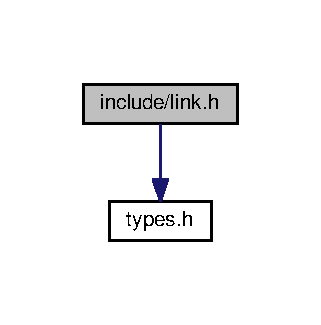
\includegraphics[width=154pt]{link_8h__incl}
\end{center}
\end{figure}
This graph shows which files directly or indirectly include this file\+:\nopagebreak
\begin{figure}[H]
\begin{center}
\leavevmode
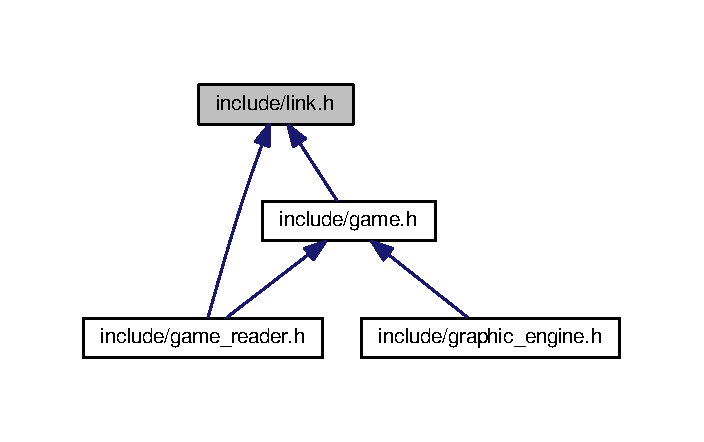
\includegraphics[width=338pt]{link_8h__dep__incl}
\end{center}
\end{figure}
\subsection*{Typedefs}
\begin{DoxyCompactItemize}
\item 
typedef struct \+\_\+\+Link \hyperlink{link_8h_ae3b299941e67be6971bfd64a25505eff}{Link}\hypertarget{link_8h_ae3b299941e67be6971bfd64a25505eff}{}\label{link_8h_ae3b299941e67be6971bfd64a25505eff}

\begin{DoxyCompactList}\small\item\em It holds the necessary data to manage a link. \end{DoxyCompactList}\end{DoxyCompactItemize}
\subsection*{Functions}
\begin{Indent}{\bf link\+\_\+create}\par
{\em It creates a link with the id passed.

\begin{DoxyAuthor}{Author}
Víctor Yrazusta 
\end{DoxyAuthor}
\begin{DoxyVersion}{Version}
1.\+0 
\end{DoxyVersion}
\begin{DoxyDate}{Date}
26-\/03-\/2018 
\end{DoxyDate}

\begin{DoxyParams}{Parameters}
{\em Id} & -\/$>$ the id for the new link. \\
\hline
\end{DoxyParams}
\begin{DoxyReturn}{Returns}
A Link$\ast$, which points towards the created link. 
\end{DoxyReturn}
}\begin{DoxyCompactItemize}
\item 
\hyperlink{link_8h_ae3b299941e67be6971bfd64a25505eff}{Link} $\ast$ {\bfseries link\+\_\+create} (\hyperlink{types_8h_a845e604fb28f7e3d97549da3448149d3}{Id})\hypertarget{link_8h_ae5986501818a720e4295dc5e634d27f1}{}\label{link_8h_ae5986501818a720e4295dc5e634d27f1}

\end{DoxyCompactItemize}
\end{Indent}
\begin{Indent}{\bf link\+\_\+destroy}\par
{\em It destroys the link passed.

\begin{DoxyAuthor}{Author}
Víctor Yrazusta 
\end{DoxyAuthor}
\begin{DoxyVersion}{Version}
1.\+0 
\end{DoxyVersion}
\begin{DoxyDate}{Date}
26-\/03-\/2018 
\end{DoxyDate}

\begin{DoxyParams}{Parameters}
{\em Link$\ast$} & -\/$>$ the link which will be destroyed. \\
\hline
\end{DoxyParams}
\begin{DoxyReturn}{Returns}
A S\+T\+A\+T\+US which indicates whether the operation could be executed correctly. 
\end{DoxyReturn}
}\begin{DoxyCompactItemize}
\item 
\hyperlink{types_8h_a32c27cc471df37f4fc818d65de0a56c4}{S\+T\+A\+T\+US} {\bfseries link\+\_\+destroy} (\hyperlink{link_8h_ae3b299941e67be6971bfd64a25505eff}{Link} $\ast$)\hypertarget{link_8h_a6f92a24607b7304bf1948b15795b2ec3}{}\label{link_8h_a6f92a24607b7304bf1948b15795b2ec3}

\end{DoxyCompactItemize}
\end{Indent}
\begin{Indent}{\bf link\+\_\+set\+\_\+name}\par
{\em It changes the name of the passed link.

\begin{DoxyAuthor}{Author}
Víctor Yrazusta 
\end{DoxyAuthor}
\begin{DoxyVersion}{Version}
1.\+0 
\end{DoxyVersion}
\begin{DoxyDate}{Date}
26-\/03-\/2018 
\end{DoxyDate}

\begin{DoxyParams}{Parameters}
{\em Link$\ast$} & -\/$>$ the link whose name will be changed. \\
\hline
{\em char} & -\/$>$ a string with the new name for the link. \\
\hline
\end{DoxyParams}
\begin{DoxyReturn}{Returns}
A S\+T\+A\+T\+US which indicates whether the operation could be executed correctly. 
\end{DoxyReturn}
}\begin{DoxyCompactItemize}
\item 
\hyperlink{types_8h_a32c27cc471df37f4fc818d65de0a56c4}{S\+T\+A\+T\+US} {\bfseries link\+\_\+set\+\_\+name} (\hyperlink{link_8h_ae3b299941e67be6971bfd64a25505eff}{Link} $\ast$, char name\mbox{[}\hyperlink{types_8h_ac7c0207aa5a0e10d378be03b68041350}{M\+A\+X\+\_\+\+N\+A\+ME}\mbox{]})\hypertarget{link_8h_ab5c8bf7b75bcbb8ab765d9cc1f2ca4ba}{}\label{link_8h_ab5c8bf7b75bcbb8ab765d9cc1f2ca4ba}

\end{DoxyCompactItemize}
\end{Indent}
\begin{Indent}{\bf link\+\_\+add\+\_\+space}\par
{\em It adds a new space in a link.

\begin{DoxyAuthor}{Author}
Víctor Yrazusta 
\end{DoxyAuthor}
\begin{DoxyVersion}{Version}
1.\+0 
\end{DoxyVersion}
\begin{DoxyDate}{Date}
26-\/03-\/2018 
\end{DoxyDate}

\begin{DoxyParams}{Parameters}
{\em Link$\ast$} & -\/$>$ the link in which the space will be inserted. \\
\hline
{\em Id} & -\/$>$ the Id of the space to be inserted. \\
\hline
\end{DoxyParams}
\begin{DoxyReturn}{Returns}
A S\+T\+A\+T\+US which indicates whether the operation could be executed correctly. 
\end{DoxyReturn}
}\begin{DoxyCompactItemize}
\item 
\hyperlink{types_8h_a32c27cc471df37f4fc818d65de0a56c4}{S\+T\+A\+T\+US} {\bfseries link\+\_\+add\+\_\+space} (\hyperlink{link_8h_ae3b299941e67be6971bfd64a25505eff}{Link} $\ast$, \hyperlink{types_8h_a845e604fb28f7e3d97549da3448149d3}{Id})\hypertarget{link_8h_a6016af52783286d2e7abc1e21c4e350d}{}\label{link_8h_a6016af52783286d2e7abc1e21c4e350d}

\end{DoxyCompactItemize}
\end{Indent}
\begin{Indent}{\bf link\+\_\+set\+\_\+status}\par
{\em It changes the status of the link.

\begin{DoxyAuthor}{Author}
Víctor Yrazusta 
\end{DoxyAuthor}
\begin{DoxyVersion}{Version}
1.\+0 
\end{DoxyVersion}
\begin{DoxyDate}{Date}
26-\/03-\/2018 
\end{DoxyDate}

\begin{DoxyParams}{Parameters}
{\em Link$\ast$} & -\/$>$ the link whose status will be changed. \\
\hline
{\em L\+I\+N\+K\+\_\+\+S\+T\+A\+T\+US} & -\/$>$ the new status for the link. \\
\hline
\end{DoxyParams}
\begin{DoxyReturn}{Returns}
A S\+T\+A\+T\+US which indicates whether the operation could be executed correctly. 
\end{DoxyReturn}
}\begin{DoxyCompactItemize}
\item 
\hyperlink{types_8h_a32c27cc471df37f4fc818d65de0a56c4}{S\+T\+A\+T\+US} {\bfseries link\+\_\+set\+\_\+status} (\hyperlink{link_8h_ae3b299941e67be6971bfd64a25505eff}{Link} $\ast$, \hyperlink{types_8h_ab0ce7873e5a1bd8bc18fafaaed449b24}{L\+I\+N\+K\+\_\+\+S\+T\+A\+T\+US} status)\hypertarget{link_8h_a87504cf04432e9d585f0b786d0cadf4c}{}\label{link_8h_a87504cf04432e9d585f0b786d0cadf4c}

\end{DoxyCompactItemize}
\end{Indent}
\begin{Indent}{\bf link\+\_\+get\+\_\+id}\par
{\em It returns the Id of the passed link.

\begin{DoxyAuthor}{Author}
Víctor Yrazusta 
\end{DoxyAuthor}
\begin{DoxyVersion}{Version}
1.\+0 
\end{DoxyVersion}
\begin{DoxyDate}{Date}
26-\/03-\/2018 
\end{DoxyDate}

\begin{DoxyParams}{Parameters}
{\em Link$\ast$} & -\/$>$ the link whose Id will be returned. \\
\hline
\end{DoxyParams}
\begin{DoxyReturn}{Returns}
An Id of the link passed. 
\end{DoxyReturn}
}\begin{DoxyCompactItemize}
\item 
\hyperlink{types_8h_a845e604fb28f7e3d97549da3448149d3}{Id} {\bfseries link\+\_\+get\+\_\+id} (\hyperlink{link_8h_ae3b299941e67be6971bfd64a25505eff}{Link} $\ast$)\hypertarget{link_8h_adccafd8e077d74b58e73f5ab39c10fda}{}\label{link_8h_adccafd8e077d74b58e73f5ab39c10fda}

\end{DoxyCompactItemize}
\end{Indent}
\begin{Indent}{\bf link\+\_\+get\+\_\+name}\par
{\em It returns the name of the passed link.

\begin{DoxyAuthor}{Author}
Víctor Yrazusta 
\end{DoxyAuthor}
\begin{DoxyVersion}{Version}
1.\+0 
\end{DoxyVersion}
\begin{DoxyDate}{Date}
26-\/03-\/2018 
\end{DoxyDate}

\begin{DoxyParams}{Parameters}
{\em Link$\ast$} & -\/$>$ the link whose name will be returned. \\
\hline
\end{DoxyParams}
\begin{DoxyReturn}{Returns}
A char with the name of the link passed. 
\end{DoxyReturn}
}\begin{DoxyCompactItemize}
\item 
char $\ast$ {\bfseries link\+\_\+get\+\_\+name} (\hyperlink{link_8h_ae3b299941e67be6971bfd64a25505eff}{Link} $\ast$)\hypertarget{link_8h_abfbc5ea744d8b7ef27e974a9d1e96401}{}\label{link_8h_abfbc5ea744d8b7ef27e974a9d1e96401}

\end{DoxyCompactItemize}
\end{Indent}
\begin{Indent}{\bf link\+\_\+get\+\_\+other\+\_\+side}\par
{\em It returns the Id of the other side of a link.

\begin{DoxyAuthor}{Author}
Víctor Yrazusta 
\end{DoxyAuthor}
\begin{DoxyVersion}{Version}
1.\+0 
\end{DoxyVersion}
\begin{DoxyDate}{Date}
26-\/03-\/2018 
\end{DoxyDate}

\begin{DoxyParams}{Parameters}
{\em Link$\ast$} & -\/$>$ the link in which the other space will be searched. \\
\hline
{\em Id} & -\/$>$ Id of the space of one side of the link. \\
\hline
\end{DoxyParams}
\begin{DoxyReturn}{Returns}
An Id of the space of the side oposing the passed Id. 
\end{DoxyReturn}
}\begin{DoxyCompactItemize}
\item 
\hyperlink{types_8h_a845e604fb28f7e3d97549da3448149d3}{Id} {\bfseries link\+\_\+get\+\_\+other\+\_\+side} (\hyperlink{link_8h_ae3b299941e67be6971bfd64a25505eff}{Link} $\ast$, \hyperlink{types_8h_a845e604fb28f7e3d97549da3448149d3}{Id})\hypertarget{link_8h_af4c1889bee64a6ac28c0edc4880580a5}{}\label{link_8h_af4c1889bee64a6ac28c0edc4880580a5}

\end{DoxyCompactItemize}
\end{Indent}
\begin{Indent}{\bf link\+\_\+get\+\_\+status}\par
{\em It returns the status of the link passed.

\begin{DoxyAuthor}{Author}
Víctor Yrazusta 
\end{DoxyAuthor}
\begin{DoxyVersion}{Version}
1.\+0 
\end{DoxyVersion}
\begin{DoxyDate}{Date}
26-\/03-\/2018 
\end{DoxyDate}

\begin{DoxyParams}{Parameters}
{\em Link$\ast$} & -\/$>$ the link whose status will be returned. \\
\hline
\end{DoxyParams}
\begin{DoxyReturn}{Returns}
A S\+T\+A\+T\+US of the link passed. 
\end{DoxyReturn}
}\begin{DoxyCompactItemize}
\item 
\hyperlink{types_8h_ab0ce7873e5a1bd8bc18fafaaed449b24}{L\+I\+N\+K\+\_\+\+S\+T\+A\+T\+US} {\bfseries link\+\_\+get\+\_\+status} (\hyperlink{link_8h_ae3b299941e67be6971bfd64a25505eff}{Link} $\ast$)\hypertarget{link_8h_a9240bcf106709443f9f69ce563ea9ef6}{}\label{link_8h_a9240bcf106709443f9f69ce563ea9ef6}

\end{DoxyCompactItemize}
\end{Indent}
\begin{Indent}{\bf link\+\_\+print}\par
{\em It prints on the standard output all the data that hold the link passed.

\begin{DoxyAuthor}{Author}
Víctor Yrazusta 
\end{DoxyAuthor}
\begin{DoxyVersion}{Version}
1.\+0 
\end{DoxyVersion}
\begin{DoxyDate}{Date}
26-\/03-\/2018 
\end{DoxyDate}

\begin{DoxyParams}{Parameters}
{\em Link$\ast$} & -\/$>$ the link whose data will be printed. \\
\hline
\end{DoxyParams}
\begin{DoxyReturn}{Returns}
A S\+T\+A\+T\+US which indicates whether the operation could be executed correctly.
\end{DoxyReturn}
N\+O\+TE\+: This function was created for debugging purposes only and it is not used in the normal execution of the game. }\begin{DoxyCompactItemize}
\item 
\hyperlink{types_8h_a32c27cc471df37f4fc818d65de0a56c4}{S\+T\+A\+T\+US} {\bfseries link\+\_\+print} (\hyperlink{link_8h_ae3b299941e67be6971bfd64a25505eff}{Link} $\ast$)\hypertarget{link_8h_aeabb8b5956d460d0e246d5917478877a}{}\label{link_8h_aeabb8b5956d460d0e246d5917478877a}

\end{DoxyCompactItemize}
\end{Indent}


\subsection{Detailed Description}
It defines a link and the different functions it needs to be managed. 

\begin{DoxyAuthor}{Author}
Víctor Yrazusta 
\end{DoxyAuthor}
\begin{DoxyVersion}{Version}
2.\+0 
\end{DoxyVersion}
\begin{DoxyDate}{Date}
26-\/03-\/2018 (creation) 26-\/03-\/2018 (last edit) 
\end{DoxyDate}
\begin{DoxyCopyright}{Copyright}
G\+NU Public License 
\end{DoxyCopyright}

\hypertarget{link__test_8h}{}\section{include/link\+\_\+test.h File Reference}
\label{link__test_8h}\index{include/link\+\_\+test.\+h@{include/link\+\_\+test.\+h}}


It declares the tests for the test module.  


\subsection*{Functions}
\begin{DoxyCompactItemize}
\item 
void \hyperlink{link__test_8h_a82c5ee441ad22caad8272212a9e9cc26}{test1\+\_\+link\+\_\+create} ()
\item 
void \hyperlink{link__test_8h_a24b5463da176c3e578b0a0fa8bb1f9f0}{test2\+\_\+link\+\_\+create} ()
\item 
void \hyperlink{link__test_8h_a8064d57d2dea4a7554fa1b29ad8eca8a}{test3\+\_\+link\+\_\+create} ()
\item 
void \hyperlink{link__test_8h_a159475c79eaec945c64ec6da610a89a0}{test4\+\_\+link\+\_\+create} ()
\item 
void \hyperlink{link__test_8h_ae0e478a0540bed26befc071591e3ff6c}{test1\+\_\+link\+\_\+set\+\_\+name} ()
\item 
void \hyperlink{link__test_8h_aa66c1e991620a5a758ba6e4d6b4a8b73}{test2\+\_\+link\+\_\+set\+\_\+name} ()
\item 
void \hyperlink{link__test_8h_a8396e33f601deb52c940cb89cd7c6bfe}{test3\+\_\+link\+\_\+set\+\_\+name} ()
\item 
void \hyperlink{link__test_8h_af84ec726ff74021eff3ccc9c3116a634}{test1\+\_\+link\+\_\+add\+\_\+space} ()
\item 
void \hyperlink{link__test_8h_a1a9f0d8d05848f9cc3f9f30097ca9452}{test2\+\_\+link\+\_\+add\+\_\+space} ()
\item 
void \hyperlink{link__test_8h_a1fdabc1833331e2d0c3ab3e420db4a0c}{test3\+\_\+link\+\_\+add\+\_\+space} ()
\item 
void \hyperlink{link__test_8h_a3b39fdba0c3c967716572bfb01beec27}{test1\+\_\+link\+\_\+set\+\_\+status} ()
\item 
void \hyperlink{link__test_8h_a315ea19cd24434d2153b5df9f372a561}{test2\+\_\+link\+\_\+set\+\_\+status} ()
\item 
void \hyperlink{link__test_8h_a19c70f79fd51d123173f7aaf6ae50bf8}{test1\+\_\+link\+\_\+get\+\_\+id} ()
\item 
void \hyperlink{link__test_8h_a0f967a1782dd7264e73ad428d22d125d}{test2\+\_\+link\+\_\+get\+\_\+id} ()
\item 
void \hyperlink{link__test_8h_a044128db00a5cc385d7157dea8bdf3c3}{test1\+\_\+link\+\_\+get\+\_\+name} ()
\item 
void \hyperlink{link__test_8h_a4efc6cfcdc210e2803f9d285734c571e}{test2\+\_\+link\+\_\+get\+\_\+name} ()
\item 
void \hyperlink{link__test_8h_a9f7bf73b9398d551c64f6c845e9e1560}{test1\+\_\+link\+\_\+get\+\_\+status} ()
\item 
void \hyperlink{link__test_8h_a7d1062febd832b21e69df5f071425b4c}{test2\+\_\+link\+\_\+get\+\_\+status} ()
\item 
void \hyperlink{link__test_8h_a342f65b583bf77b00715e4f76c63c84f}{test1\+\_\+link\+\_\+get\+\_\+other\+\_\+side} ()
\item 
void \hyperlink{link__test_8h_a9bb64e905b519d629239c31029ec4cd2}{test2\+\_\+link\+\_\+get\+\_\+other\+\_\+side} ()
\item 
void \hyperlink{link__test_8h_a624e83e69b76d04ac199a51741a392f5}{test3\+\_\+link\+\_\+get\+\_\+other\+\_\+side} ()
\item 
void \hyperlink{link__test_8h_ad4ca02e93472a080362a005ea4840218}{test1\+\_\+link\+\_\+destroy} ()
\item 
void \hyperlink{link__test_8h_afae7294e1213cade145448511cfae536}{test2\+\_\+link\+\_\+destroy} ()
\end{DoxyCompactItemize}


\subsection{Detailed Description}
It declares the tests for the test module. 

\begin{DoxyAuthor}{Author}
Victor Yrazusta 
\end{DoxyAuthor}
\begin{DoxyVersion}{Version}
1.\+0 
\end{DoxyVersion}
\begin{DoxyDate}{Date}
05-\/03-\/2018 (creation) 
\end{DoxyDate}
\begin{DoxyCopyright}{Copyright}
G\+NU Public License 
\end{DoxyCopyright}


\subsection{Function Documentation}
\index{link\+\_\+test.\+h@{link\+\_\+test.\+h}!test1\+\_\+link\+\_\+add\+\_\+space@{test1\+\_\+link\+\_\+add\+\_\+space}}
\index{test1\+\_\+link\+\_\+add\+\_\+space@{test1\+\_\+link\+\_\+add\+\_\+space}!link\+\_\+test.\+h@{link\+\_\+test.\+h}}
\subsubsection[{\texorpdfstring{test1\+\_\+link\+\_\+add\+\_\+space()}{test1_link_add_space()}}]{\setlength{\rightskip}{0pt plus 5cm}void test1\+\_\+link\+\_\+add\+\_\+space (
\begin{DoxyParamCaption}
{}
\end{DoxyParamCaption}
)}\hypertarget{link__test_8h_af84ec726ff74021eff3ccc9c3116a634}{}\label{link__test_8h_af84ec726ff74021eff3ccc9c3116a634}
\begin{DoxyRefDesc}{Test}
\item[\hyperlink{test__test000130}{Test}]Test function for link-\/$>$space1 and link-\/$>$space2 settings \end{DoxyRefDesc}
\begin{DoxyPrecond}{Precondition}
Two correct Space I\+Ds 
\end{DoxyPrecond}
\begin{DoxyPostcond}{Postcondition}
Output == OK 
\end{DoxyPostcond}
\index{link\+\_\+test.\+h@{link\+\_\+test.\+h}!test1\+\_\+link\+\_\+create@{test1\+\_\+link\+\_\+create}}
\index{test1\+\_\+link\+\_\+create@{test1\+\_\+link\+\_\+create}!link\+\_\+test.\+h@{link\+\_\+test.\+h}}
\subsubsection[{\texorpdfstring{test1\+\_\+link\+\_\+create()}{test1_link_create()}}]{\setlength{\rightskip}{0pt plus 5cm}void test1\+\_\+link\+\_\+create (
\begin{DoxyParamCaption}
{}
\end{DoxyParamCaption}
)}\hypertarget{link__test_8h_a82c5ee441ad22caad8272212a9e9cc26}{}\label{link__test_8h_a82c5ee441ad22caad8272212a9e9cc26}
\begin{DoxyRefDesc}{Test}
\item[\hyperlink{test__test000123}{Test}]Test link creation \end{DoxyRefDesc}
\begin{DoxyPrecond}{Precondition}
Link ID 
\end{DoxyPrecond}
\begin{DoxyPostcond}{Postcondition}
Non N\+U\+LL pointer to link 
\end{DoxyPostcond}
\index{link\+\_\+test.\+h@{link\+\_\+test.\+h}!test1\+\_\+link\+\_\+destroy@{test1\+\_\+link\+\_\+destroy}}
\index{test1\+\_\+link\+\_\+destroy@{test1\+\_\+link\+\_\+destroy}!link\+\_\+test.\+h@{link\+\_\+test.\+h}}
\subsubsection[{\texorpdfstring{test1\+\_\+link\+\_\+destroy()}{test1_link_destroy()}}]{\setlength{\rightskip}{0pt plus 5cm}void test1\+\_\+link\+\_\+destroy (
\begin{DoxyParamCaption}
{}
\end{DoxyParamCaption}
)}\hypertarget{link__test_8h_ad4ca02e93472a080362a005ea4840218}{}\label{link__test_8h_ad4ca02e93472a080362a005ea4840218}
\begin{DoxyRefDesc}{Test}
\item[\hyperlink{test__test000144}{Test}]Test function for destroying links \end{DoxyRefDesc}
\begin{DoxyPrecond}{Precondition}
A correct Link pointer 
\end{DoxyPrecond}
\begin{DoxyPostcond}{Postcondition}
Output == OK 
\end{DoxyPostcond}
\index{link\+\_\+test.\+h@{link\+\_\+test.\+h}!test1\+\_\+link\+\_\+get\+\_\+id@{test1\+\_\+link\+\_\+get\+\_\+id}}
\index{test1\+\_\+link\+\_\+get\+\_\+id@{test1\+\_\+link\+\_\+get\+\_\+id}!link\+\_\+test.\+h@{link\+\_\+test.\+h}}
\subsubsection[{\texorpdfstring{test1\+\_\+link\+\_\+get\+\_\+id()}{test1_link_get_id()}}]{\setlength{\rightskip}{0pt plus 5cm}void test1\+\_\+link\+\_\+get\+\_\+id (
\begin{DoxyParamCaption}
{}
\end{DoxyParamCaption}
)}\hypertarget{link__test_8h_a19c70f79fd51d123173f7aaf6ae50bf8}{}\label{link__test_8h_a19c70f79fd51d123173f7aaf6ae50bf8}
\begin{DoxyRefDesc}{Test}
\item[\hyperlink{test__test000135}{Test}]Test function for reading link-\/$>$id setting \end{DoxyRefDesc}
\begin{DoxyPrecond}{Precondition}
A Correct Link Id 
\end{DoxyPrecond}
\begin{DoxyPostcond}{Postcondition}
Registered ID == Given ID 
\end{DoxyPostcond}
\index{link\+\_\+test.\+h@{link\+\_\+test.\+h}!test1\+\_\+link\+\_\+get\+\_\+name@{test1\+\_\+link\+\_\+get\+\_\+name}}
\index{test1\+\_\+link\+\_\+get\+\_\+name@{test1\+\_\+link\+\_\+get\+\_\+name}!link\+\_\+test.\+h@{link\+\_\+test.\+h}}
\subsubsection[{\texorpdfstring{test1\+\_\+link\+\_\+get\+\_\+name()}{test1_link_get_name()}}]{\setlength{\rightskip}{0pt plus 5cm}void test1\+\_\+link\+\_\+get\+\_\+name (
\begin{DoxyParamCaption}
{}
\end{DoxyParamCaption}
)}\hypertarget{link__test_8h_a044128db00a5cc385d7157dea8bdf3c3}{}\label{link__test_8h_a044128db00a5cc385d7157dea8bdf3c3}
\begin{DoxyRefDesc}{Test}
\item[\hyperlink{test__test000137}{Test}]Test function for reading link-\/$>$name setting \end{DoxyRefDesc}
\begin{DoxyPrecond}{Precondition}
A Correct string 
\end{DoxyPrecond}
\begin{DoxyPostcond}{Postcondition}
Registered name == Given string 
\end{DoxyPostcond}
\index{link\+\_\+test.\+h@{link\+\_\+test.\+h}!test1\+\_\+link\+\_\+get\+\_\+other\+\_\+side@{test1\+\_\+link\+\_\+get\+\_\+other\+\_\+side}}
\index{test1\+\_\+link\+\_\+get\+\_\+other\+\_\+side@{test1\+\_\+link\+\_\+get\+\_\+other\+\_\+side}!link\+\_\+test.\+h@{link\+\_\+test.\+h}}
\subsubsection[{\texorpdfstring{test1\+\_\+link\+\_\+get\+\_\+other\+\_\+side()}{test1_link_get_other_side()}}]{\setlength{\rightskip}{0pt plus 5cm}void test1\+\_\+link\+\_\+get\+\_\+other\+\_\+side (
\begin{DoxyParamCaption}
{}
\end{DoxyParamCaption}
)}\hypertarget{link__test_8h_a342f65b583bf77b00715e4f76c63c84f}{}\label{link__test_8h_a342f65b583bf77b00715e4f76c63c84f}
\begin{DoxyRefDesc}{Test}
\item[\hyperlink{test__test000141}{Test}]Test function for link\+\_\+get\+\_\+other\+\_\+side \end{DoxyRefDesc}
\begin{DoxyPrecond}{Precondition}
Two correct Space I\+Ds 
\end{DoxyPrecond}
\begin{DoxyPostcond}{Postcondition}
Registered I\+Ds == Given I\+Ds 
\end{DoxyPostcond}
\index{link\+\_\+test.\+h@{link\+\_\+test.\+h}!test1\+\_\+link\+\_\+get\+\_\+status@{test1\+\_\+link\+\_\+get\+\_\+status}}
\index{test1\+\_\+link\+\_\+get\+\_\+status@{test1\+\_\+link\+\_\+get\+\_\+status}!link\+\_\+test.\+h@{link\+\_\+test.\+h}}
\subsubsection[{\texorpdfstring{test1\+\_\+link\+\_\+get\+\_\+status()}{test1_link_get_status()}}]{\setlength{\rightskip}{0pt plus 5cm}void test1\+\_\+link\+\_\+get\+\_\+status (
\begin{DoxyParamCaption}
{}
\end{DoxyParamCaption}
)}\hypertarget{link__test_8h_a9f7bf73b9398d551c64f6c845e9e1560}{}\label{link__test_8h_a9f7bf73b9398d551c64f6c845e9e1560}
\begin{DoxyRefDesc}{Test}
\item[\hyperlink{test__test000139}{Test}]Test function for reading link-\/$>$status setting \end{DoxyRefDesc}
\begin{DoxyPrecond}{Precondition}
A correct Link pointer 
\end{DoxyPrecond}
\begin{DoxyPostcond}{Postcondition}
Registered status == Given status 
\end{DoxyPostcond}
\index{link\+\_\+test.\+h@{link\+\_\+test.\+h}!test1\+\_\+link\+\_\+set\+\_\+name@{test1\+\_\+link\+\_\+set\+\_\+name}}
\index{test1\+\_\+link\+\_\+set\+\_\+name@{test1\+\_\+link\+\_\+set\+\_\+name}!link\+\_\+test.\+h@{link\+\_\+test.\+h}}
\subsubsection[{\texorpdfstring{test1\+\_\+link\+\_\+set\+\_\+name()}{test1_link_set_name()}}]{\setlength{\rightskip}{0pt plus 5cm}void test1\+\_\+link\+\_\+set\+\_\+name (
\begin{DoxyParamCaption}
{}
\end{DoxyParamCaption}
)}\hypertarget{link__test_8h_ae0e478a0540bed26befc071591e3ff6c}{}\label{link__test_8h_ae0e478a0540bed26befc071591e3ff6c}
\begin{DoxyRefDesc}{Test}
\item[\hyperlink{test__test000127}{Test}]Test function for link-\/$>$name setting \end{DoxyRefDesc}
\begin{DoxyPrecond}{Precondition}
A string 
\end{DoxyPrecond}
\begin{DoxyPostcond}{Postcondition}
Output == OK 
\end{DoxyPostcond}
\index{link\+\_\+test.\+h@{link\+\_\+test.\+h}!test1\+\_\+link\+\_\+set\+\_\+status@{test1\+\_\+link\+\_\+set\+\_\+status}}
\index{test1\+\_\+link\+\_\+set\+\_\+status@{test1\+\_\+link\+\_\+set\+\_\+status}!link\+\_\+test.\+h@{link\+\_\+test.\+h}}
\subsubsection[{\texorpdfstring{test1\+\_\+link\+\_\+set\+\_\+status()}{test1_link_set_status()}}]{\setlength{\rightskip}{0pt plus 5cm}void test1\+\_\+link\+\_\+set\+\_\+status (
\begin{DoxyParamCaption}
{}
\end{DoxyParamCaption}
)}\hypertarget{link__test_8h_a3b39fdba0c3c967716572bfb01beec27}{}\label{link__test_8h_a3b39fdba0c3c967716572bfb01beec27}
\begin{DoxyRefDesc}{Test}
\item[\hyperlink{test__test000133}{Test}]Test function for link-\/$>$status setting \end{DoxyRefDesc}
\begin{DoxyPrecond}{Precondition}
A link status 
\end{DoxyPrecond}
\begin{DoxyPostcond}{Postcondition}
Output == OK 
\end{DoxyPostcond}
\index{link\+\_\+test.\+h@{link\+\_\+test.\+h}!test2\+\_\+link\+\_\+add\+\_\+space@{test2\+\_\+link\+\_\+add\+\_\+space}}
\index{test2\+\_\+link\+\_\+add\+\_\+space@{test2\+\_\+link\+\_\+add\+\_\+space}!link\+\_\+test.\+h@{link\+\_\+test.\+h}}
\subsubsection[{\texorpdfstring{test2\+\_\+link\+\_\+add\+\_\+space()}{test2_link_add_space()}}]{\setlength{\rightskip}{0pt plus 5cm}void test2\+\_\+link\+\_\+add\+\_\+space (
\begin{DoxyParamCaption}
{}
\end{DoxyParamCaption}
)}\hypertarget{link__test_8h_a1a9f0d8d05848f9cc3f9f30097ca9452}{}\label{link__test_8h_a1a9f0d8d05848f9cc3f9f30097ca9452}
\begin{DoxyRefDesc}{Test}
\item[\hyperlink{test__test000131}{Test}]Test function for link-\/$>$space1 and link-\/$>$space2 settings \end{DoxyRefDesc}
\begin{DoxyPrecond}{Precondition}
One correct Space ID amd one incorrect 
\end{DoxyPrecond}
\begin{DoxyPostcond}{Postcondition}
Output == E\+R\+R\+OR for the incorrect one and == OK for the correct one 
\end{DoxyPostcond}
\index{link\+\_\+test.\+h@{link\+\_\+test.\+h}!test2\+\_\+link\+\_\+create@{test2\+\_\+link\+\_\+create}}
\index{test2\+\_\+link\+\_\+create@{test2\+\_\+link\+\_\+create}!link\+\_\+test.\+h@{link\+\_\+test.\+h}}
\subsubsection[{\texorpdfstring{test2\+\_\+link\+\_\+create()}{test2_link_create()}}]{\setlength{\rightskip}{0pt plus 5cm}void test2\+\_\+link\+\_\+create (
\begin{DoxyParamCaption}
{}
\end{DoxyParamCaption}
)}\hypertarget{link__test_8h_a24b5463da176c3e578b0a0fa8bb1f9f0}{}\label{link__test_8h_a24b5463da176c3e578b0a0fa8bb1f9f0}
\begin{DoxyRefDesc}{Test}
\item[\hyperlink{test__test000124}{Test}]Test link creation \end{DoxyRefDesc}
\begin{DoxyPrecond}{Precondition}
Link ID 
\end{DoxyPrecond}
\begin{DoxyPostcond}{Postcondition}
Link\+\_\+\+ID == Supplied Link Id 
\end{DoxyPostcond}
\index{link\+\_\+test.\+h@{link\+\_\+test.\+h}!test2\+\_\+link\+\_\+destroy@{test2\+\_\+link\+\_\+destroy}}
\index{test2\+\_\+link\+\_\+destroy@{test2\+\_\+link\+\_\+destroy}!link\+\_\+test.\+h@{link\+\_\+test.\+h}}
\subsubsection[{\texorpdfstring{test2\+\_\+link\+\_\+destroy()}{test2_link_destroy()}}]{\setlength{\rightskip}{0pt plus 5cm}void test2\+\_\+link\+\_\+destroy (
\begin{DoxyParamCaption}
{}
\end{DoxyParamCaption}
)}\hypertarget{link__test_8h_afae7294e1213cade145448511cfae536}{}\label{link__test_8h_afae7294e1213cade145448511cfae536}
\begin{DoxyRefDesc}{Test}
\item[\hyperlink{test__test000145}{Test}]Test function for destroying links \end{DoxyRefDesc}
\begin{DoxyPrecond}{Precondition}
A N\+U\+LL Link pointer 
\end{DoxyPrecond}
\begin{DoxyPostcond}{Postcondition}
Output == E\+R\+R\+OR 
\end{DoxyPostcond}
\index{link\+\_\+test.\+h@{link\+\_\+test.\+h}!test2\+\_\+link\+\_\+get\+\_\+id@{test2\+\_\+link\+\_\+get\+\_\+id}}
\index{test2\+\_\+link\+\_\+get\+\_\+id@{test2\+\_\+link\+\_\+get\+\_\+id}!link\+\_\+test.\+h@{link\+\_\+test.\+h}}
\subsubsection[{\texorpdfstring{test2\+\_\+link\+\_\+get\+\_\+id()}{test2_link_get_id()}}]{\setlength{\rightskip}{0pt plus 5cm}void test2\+\_\+link\+\_\+get\+\_\+id (
\begin{DoxyParamCaption}
{}
\end{DoxyParamCaption}
)}\hypertarget{link__test_8h_a0f967a1782dd7264e73ad428d22d125d}{}\label{link__test_8h_a0f967a1782dd7264e73ad428d22d125d}
\begin{DoxyRefDesc}{Test}
\item[\hyperlink{test__test000136}{Test}]Test function for reading link-\/$>$id setting \end{DoxyRefDesc}
\begin{DoxyPrecond}{Precondition}
A N\+U\+LL Link pointer 
\end{DoxyPrecond}
\begin{DoxyPostcond}{Postcondition}
Output == N\+O\+\_\+\+ID 
\end{DoxyPostcond}
\index{link\+\_\+test.\+h@{link\+\_\+test.\+h}!test2\+\_\+link\+\_\+get\+\_\+name@{test2\+\_\+link\+\_\+get\+\_\+name}}
\index{test2\+\_\+link\+\_\+get\+\_\+name@{test2\+\_\+link\+\_\+get\+\_\+name}!link\+\_\+test.\+h@{link\+\_\+test.\+h}}
\subsubsection[{\texorpdfstring{test2\+\_\+link\+\_\+get\+\_\+name()}{test2_link_get_name()}}]{\setlength{\rightskip}{0pt plus 5cm}void test2\+\_\+link\+\_\+get\+\_\+name (
\begin{DoxyParamCaption}
{}
\end{DoxyParamCaption}
)}\hypertarget{link__test_8h_a4efc6cfcdc210e2803f9d285734c571e}{}\label{link__test_8h_a4efc6cfcdc210e2803f9d285734c571e}
\begin{DoxyRefDesc}{Test}
\item[\hyperlink{test__test000138}{Test}]Test function for reading link-\/$>$name setting \end{DoxyRefDesc}
\begin{DoxyPrecond}{Precondition}
A N\+U\+LL Link pointer 
\end{DoxyPrecond}
\begin{DoxyPostcond}{Postcondition}
Registered name == N\+U\+LL 
\end{DoxyPostcond}
\index{link\+\_\+test.\+h@{link\+\_\+test.\+h}!test2\+\_\+link\+\_\+get\+\_\+other\+\_\+side@{test2\+\_\+link\+\_\+get\+\_\+other\+\_\+side}}
\index{test2\+\_\+link\+\_\+get\+\_\+other\+\_\+side@{test2\+\_\+link\+\_\+get\+\_\+other\+\_\+side}!link\+\_\+test.\+h@{link\+\_\+test.\+h}}
\subsubsection[{\texorpdfstring{test2\+\_\+link\+\_\+get\+\_\+other\+\_\+side()}{test2_link_get_other_side()}}]{\setlength{\rightskip}{0pt plus 5cm}void test2\+\_\+link\+\_\+get\+\_\+other\+\_\+side (
\begin{DoxyParamCaption}
{}
\end{DoxyParamCaption}
)}\hypertarget{link__test_8h_a9bb64e905b519d629239c31029ec4cd2}{}\label{link__test_8h_a9bb64e905b519d629239c31029ec4cd2}
\begin{DoxyRefDesc}{Test}
\item[\hyperlink{test__test000142}{Test}]Test function for link\+\_\+get\+\_\+other\+\_\+side \end{DoxyRefDesc}
\begin{DoxyPrecond}{Precondition}
One correct Space ID and one incorrect 
\end{DoxyPrecond}
\begin{DoxyPostcond}{Postcondition}
Registered I\+Ds != Given I\+Ds 
\end{DoxyPostcond}
\index{link\+\_\+test.\+h@{link\+\_\+test.\+h}!test2\+\_\+link\+\_\+get\+\_\+status@{test2\+\_\+link\+\_\+get\+\_\+status}}
\index{test2\+\_\+link\+\_\+get\+\_\+status@{test2\+\_\+link\+\_\+get\+\_\+status}!link\+\_\+test.\+h@{link\+\_\+test.\+h}}
\subsubsection[{\texorpdfstring{test2\+\_\+link\+\_\+get\+\_\+status()}{test2_link_get_status()}}]{\setlength{\rightskip}{0pt plus 5cm}void test2\+\_\+link\+\_\+get\+\_\+status (
\begin{DoxyParamCaption}
{}
\end{DoxyParamCaption}
)}\hypertarget{link__test_8h_a7d1062febd832b21e69df5f071425b4c}{}\label{link__test_8h_a7d1062febd832b21e69df5f071425b4c}
\begin{DoxyRefDesc}{Test}
\item[\hyperlink{test__test000140}{Test}]Test function for reading link-\/$>$status setting \end{DoxyRefDesc}
\begin{DoxyPrecond}{Precondition}
A incorrect Link pointer 
\end{DoxyPrecond}
\begin{DoxyPostcond}{Postcondition}
Registered status != Given status 
\end{DoxyPostcond}
\index{link\+\_\+test.\+h@{link\+\_\+test.\+h}!test2\+\_\+link\+\_\+set\+\_\+name@{test2\+\_\+link\+\_\+set\+\_\+name}}
\index{test2\+\_\+link\+\_\+set\+\_\+name@{test2\+\_\+link\+\_\+set\+\_\+name}!link\+\_\+test.\+h@{link\+\_\+test.\+h}}
\subsubsection[{\texorpdfstring{test2\+\_\+link\+\_\+set\+\_\+name()}{test2_link_set_name()}}]{\setlength{\rightskip}{0pt plus 5cm}void test2\+\_\+link\+\_\+set\+\_\+name (
\begin{DoxyParamCaption}
{}
\end{DoxyParamCaption}
)}\hypertarget{link__test_8h_aa66c1e991620a5a758ba6e4d6b4a8b73}{}\label{link__test_8h_aa66c1e991620a5a758ba6e4d6b4a8b73}
\begin{DoxyRefDesc}{Test}
\item[\hyperlink{test__test000128}{Test}]Test function for link-\/$>$name setting \end{DoxyRefDesc}
\begin{DoxyPrecond}{Precondition}
A null link pointer 
\end{DoxyPrecond}
\begin{DoxyPostcond}{Postcondition}
Output == E\+R\+R\+OR 
\end{DoxyPostcond}
\index{link\+\_\+test.\+h@{link\+\_\+test.\+h}!test2\+\_\+link\+\_\+set\+\_\+status@{test2\+\_\+link\+\_\+set\+\_\+status}}
\index{test2\+\_\+link\+\_\+set\+\_\+status@{test2\+\_\+link\+\_\+set\+\_\+status}!link\+\_\+test.\+h@{link\+\_\+test.\+h}}
\subsubsection[{\texorpdfstring{test2\+\_\+link\+\_\+set\+\_\+status()}{test2_link_set_status()}}]{\setlength{\rightskip}{0pt plus 5cm}void test2\+\_\+link\+\_\+set\+\_\+status (
\begin{DoxyParamCaption}
{}
\end{DoxyParamCaption}
)}\hypertarget{link__test_8h_a315ea19cd24434d2153b5df9f372a561}{}\label{link__test_8h_a315ea19cd24434d2153b5df9f372a561}
\begin{DoxyRefDesc}{Test}
\item[\hyperlink{test__test000134}{Test}]Test function for link-\/$>$status setting \end{DoxyRefDesc}
\begin{DoxyPrecond}{Precondition}
A N\+U\+LL Link pointer 
\end{DoxyPrecond}
\begin{DoxyPostcond}{Postcondition}
Output == E\+R\+R\+OR 
\end{DoxyPostcond}
\index{link\+\_\+test.\+h@{link\+\_\+test.\+h}!test3\+\_\+link\+\_\+add\+\_\+space@{test3\+\_\+link\+\_\+add\+\_\+space}}
\index{test3\+\_\+link\+\_\+add\+\_\+space@{test3\+\_\+link\+\_\+add\+\_\+space}!link\+\_\+test.\+h@{link\+\_\+test.\+h}}
\subsubsection[{\texorpdfstring{test3\+\_\+link\+\_\+add\+\_\+space()}{test3_link_add_space()}}]{\setlength{\rightskip}{0pt plus 5cm}void test3\+\_\+link\+\_\+add\+\_\+space (
\begin{DoxyParamCaption}
{}
\end{DoxyParamCaption}
)}\hypertarget{link__test_8h_a1fdabc1833331e2d0c3ab3e420db4a0c}{}\label{link__test_8h_a1fdabc1833331e2d0c3ab3e420db4a0c}
\begin{DoxyRefDesc}{Test}
\item[\hyperlink{test__test000132}{Test}]Test function for link-\/$>$space1 and link-\/$>$space2 settings \end{DoxyRefDesc}
\begin{DoxyPrecond}{Precondition}
A N\+U\+LL Link pointer 
\end{DoxyPrecond}
\begin{DoxyPostcond}{Postcondition}
Output == E\+R\+R\+OR 
\end{DoxyPostcond}
\index{link\+\_\+test.\+h@{link\+\_\+test.\+h}!test3\+\_\+link\+\_\+create@{test3\+\_\+link\+\_\+create}}
\index{test3\+\_\+link\+\_\+create@{test3\+\_\+link\+\_\+create}!link\+\_\+test.\+h@{link\+\_\+test.\+h}}
\subsubsection[{\texorpdfstring{test3\+\_\+link\+\_\+create()}{test3_link_create()}}]{\setlength{\rightskip}{0pt plus 5cm}void test3\+\_\+link\+\_\+create (
\begin{DoxyParamCaption}
{}
\end{DoxyParamCaption}
)}\hypertarget{link__test_8h_a8064d57d2dea4a7554fa1b29ad8eca8a}{}\label{link__test_8h_a8064d57d2dea4a7554fa1b29ad8eca8a}
\begin{DoxyRefDesc}{Test}
\item[\hyperlink{test__test000125}{Test}]Test link creation \end{DoxyRefDesc}
\begin{DoxyPrecond}{Precondition}
Link ID and Link Status 
\end{DoxyPrecond}
\begin{DoxyPostcond}{Postcondition}
Link\+\_\+\+ID == Supplied Link Id and Link\+\_\+\+Status == Supplied Link Status 
\end{DoxyPostcond}
\index{link\+\_\+test.\+h@{link\+\_\+test.\+h}!test3\+\_\+link\+\_\+get\+\_\+other\+\_\+side@{test3\+\_\+link\+\_\+get\+\_\+other\+\_\+side}}
\index{test3\+\_\+link\+\_\+get\+\_\+other\+\_\+side@{test3\+\_\+link\+\_\+get\+\_\+other\+\_\+side}!link\+\_\+test.\+h@{link\+\_\+test.\+h}}
\subsubsection[{\texorpdfstring{test3\+\_\+link\+\_\+get\+\_\+other\+\_\+side()}{test3_link_get_other_side()}}]{\setlength{\rightskip}{0pt plus 5cm}void test3\+\_\+link\+\_\+get\+\_\+other\+\_\+side (
\begin{DoxyParamCaption}
{}
\end{DoxyParamCaption}
)}\hypertarget{link__test_8h_a624e83e69b76d04ac199a51741a392f5}{}\label{link__test_8h_a624e83e69b76d04ac199a51741a392f5}
\begin{DoxyRefDesc}{Test}
\item[\hyperlink{test__test000143}{Test}]Test function for link\+\_\+get\+\_\+other\+\_\+side \end{DoxyRefDesc}
\begin{DoxyPrecond}{Precondition}
A N\+U\+LL Link pointer 
\end{DoxyPrecond}
\begin{DoxyPostcond}{Postcondition}
Registered I\+Ds != Given I\+Ds 
\end{DoxyPostcond}
\index{link\+\_\+test.\+h@{link\+\_\+test.\+h}!test3\+\_\+link\+\_\+set\+\_\+name@{test3\+\_\+link\+\_\+set\+\_\+name}}
\index{test3\+\_\+link\+\_\+set\+\_\+name@{test3\+\_\+link\+\_\+set\+\_\+name}!link\+\_\+test.\+h@{link\+\_\+test.\+h}}
\subsubsection[{\texorpdfstring{test3\+\_\+link\+\_\+set\+\_\+name()}{test3_link_set_name()}}]{\setlength{\rightskip}{0pt plus 5cm}void test3\+\_\+link\+\_\+set\+\_\+name (
\begin{DoxyParamCaption}
{}
\end{DoxyParamCaption}
)}\hypertarget{link__test_8h_a8396e33f601deb52c940cb89cd7c6bfe}{}\label{link__test_8h_a8396e33f601deb52c940cb89cd7c6bfe}
\begin{DoxyRefDesc}{Test}
\item[\hyperlink{test__test000129}{Test}]Test function for link-\/$>$name setting \end{DoxyRefDesc}
\begin{DoxyPrecond}{Precondition}
A null string pointer 
\end{DoxyPrecond}
\begin{DoxyPostcond}{Postcondition}
Output == E\+R\+R\+OR 
\end{DoxyPostcond}
\index{link\+\_\+test.\+h@{link\+\_\+test.\+h}!test4\+\_\+link\+\_\+create@{test4\+\_\+link\+\_\+create}}
\index{test4\+\_\+link\+\_\+create@{test4\+\_\+link\+\_\+create}!link\+\_\+test.\+h@{link\+\_\+test.\+h}}
\subsubsection[{\texorpdfstring{test4\+\_\+link\+\_\+create()}{test4_link_create()}}]{\setlength{\rightskip}{0pt plus 5cm}void test4\+\_\+link\+\_\+create (
\begin{DoxyParamCaption}
{}
\end{DoxyParamCaption}
)}\hypertarget{link__test_8h_a159475c79eaec945c64ec6da610a89a0}{}\label{link__test_8h_a159475c79eaec945c64ec6da610a89a0}
\begin{DoxyRefDesc}{Test}
\item[\hyperlink{test__test000126}{Test}]Test link creation \end{DoxyRefDesc}
\begin{DoxyPrecond}{Precondition}
Link ID and Link Status and two Space I\+Ds 
\end{DoxyPrecond}
\begin{DoxyPostcond}{Postcondition}
Link\+\_\+\+ID == Supplied Link Id and Link\+\_\+\+Status == Supplied Link Status and both Spaces\+\_\+\+I\+Ds == Supplied Space I\+Ds 
\end{DoxyPostcond}

\hypertarget{object_8h}{}\section{include/object.h File Reference}
\label{object_8h}\index{include/object.\+h@{include/object.\+h}}


It defines an object and the necessary functions to use it.  


{\ttfamily \#include \char`\"{}types.\+h\char`\"{}}\\*
Include dependency graph for object.\+h\+:\nopagebreak
\begin{figure}[H]
\begin{center}
\leavevmode
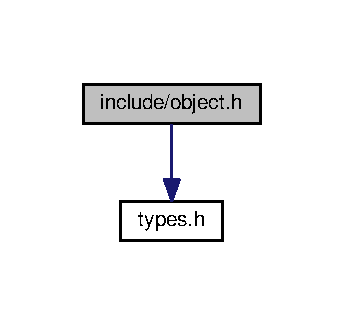
\includegraphics[width=165pt]{object_8h__incl}
\end{center}
\end{figure}
This graph shows which files directly or indirectly include this file\+:\nopagebreak
\begin{figure}[H]
\begin{center}
\leavevmode
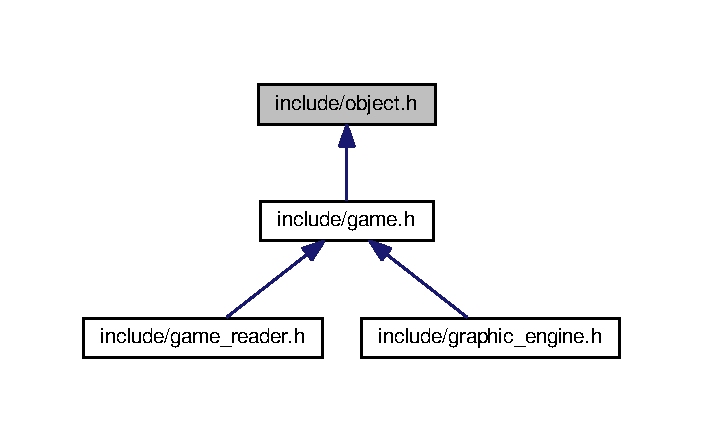
\includegraphics[width=338pt]{object_8h__dep__incl}
\end{center}
\end{figure}
\subsection*{Typedefs}
\begin{DoxyCompactItemize}
\item 
typedef struct \+\_\+\+Object \hyperlink{object_8h_a7f8bbcda919b65ce67f92fba08e0212f}{Object}\hypertarget{object_8h_a7f8bbcda919b65ce67f92fba08e0212f}{}\label{object_8h_a7f8bbcda919b65ce67f92fba08e0212f}

\begin{DoxyCompactList}\small\item\em It holds the necessary data to manage an object. \end{DoxyCompactList}\end{DoxyCompactItemize}
\subsection*{Functions}
\begin{Indent}{\bf object\+\_\+create}\par
{\em It creates an object with the id passed.

\begin{DoxyAuthor}{Author}
Alejandro Pascual edited by Eric Morales and Victor Yrazusta 
\end{DoxyAuthor}
\begin{DoxyVersion}{Version}
2.\+0 
\end{DoxyVersion}
\begin{DoxyDate}{Date}
19-\/02-\/2018 
\end{DoxyDate}

\begin{DoxyParams}{Parameters}
{\em Id} & -\/$>$ the Id of the created object. \\
\hline
\end{DoxyParams}
\begin{DoxyReturn}{Returns}
An Object$\ast$, which points towards the created object. 
\end{DoxyReturn}
}\begin{DoxyCompactItemize}
\item 
\hyperlink{object_8h_a7f8bbcda919b65ce67f92fba08e0212f}{Object} $\ast$ {\bfseries object\+\_\+create} (\hyperlink{types_8h_a845e604fb28f7e3d97549da3448149d3}{Id})\hypertarget{object_8h_a27a09fed29aed663ae056488a6e09e96}{}\label{object_8h_a27a09fed29aed663ae056488a6e09e96}

\end{DoxyCompactItemize}
\end{Indent}
\begin{Indent}{\bf object\+\_\+destroy}\par
{\em It deallocates the memory reserved for the Object$\ast$ passed.

\begin{DoxyAuthor}{Author}
Victor Yrazusta edited by Eric Morales 
\end{DoxyAuthor}
\begin{DoxyVersion}{Version}
2.\+0 
\end{DoxyVersion}
\begin{DoxyDate}{Date}
19-\/02-\/2018 
\end{DoxyDate}

\begin{DoxyParams}{Parameters}
{\em Object$\ast$} & -\/$>$ the object which will be deallocated. \\
\hline
\end{DoxyParams}
\begin{DoxyReturn}{Returns}
An S\+T\+A\+T\+US, which could be E\+R\+R\+OR if the pointer passed as an argument is N\+U\+LL, or OK otherwise. 
\end{DoxyReturn}
}\begin{DoxyCompactItemize}
\item 
\hyperlink{types_8h_a32c27cc471df37f4fc818d65de0a56c4}{S\+T\+A\+T\+US} {\bfseries object\+\_\+destroy} (\hyperlink{object_8h_a7f8bbcda919b65ce67f92fba08e0212f}{Object} $\ast$)\hypertarget{object_8h_a5f446eb95985239170cb8d2cfd00ec5a}{}\label{object_8h_a5f446eb95985239170cb8d2cfd00ec5a}

\end{DoxyCompactItemize}
\end{Indent}
\begin{Indent}{\bf object\+\_\+set\+\_\+check}\par
{\em It changes the check of the passed object to the passed char$\ast$$\ast$.

\begin{DoxyAuthor}{Author}
Eric Morales 
\end{DoxyAuthor}
\begin{DoxyVersion}{Version}
1.\+0 
\end{DoxyVersion}
\begin{DoxyDate}{Date}
26-\/03-\/2018 
\end{DoxyDate}

\begin{DoxyParams}{Parameters}
{\em Object$\ast$} & -\/$>$ which must point towards the object that wants to be renamed. \\
\hline
{\em char} & -\/$>$ a string with the new check for the object. \\
\hline
\end{DoxyParams}
\begin{DoxyReturn}{Returns}
An S\+T\+A\+T\+US, which could be \char`\"{}\+E\+R\+R\+O\+R\char`\"{} if one of the passed pointers is N\+U\+LL or if the rename fails, or \char`\"{}\+O\+K\char`\"{} otherwise. 
\end{DoxyReturn}
}\begin{DoxyCompactItemize}
\item 
\hyperlink{types_8h_a32c27cc471df37f4fc818d65de0a56c4}{S\+T\+A\+T\+US} {\bfseries object\+\_\+set\+\_\+check} (\hyperlink{object_8h_a7f8bbcda919b65ce67f92fba08e0212f}{Object} $\ast$, char check\mbox{[}\hyperlink{types_8h_ae41569a4c2560714ec2b9feb28919682}{M\+A\+X\+\_\+\+C\+H\+E\+C\+K\+\_\+R}\mbox{]}\mbox{[}\hyperlink{types_8h_a9990950cd307079021e49d95eae07c60}{M\+A\+X\+\_\+\+C\+H\+E\+C\+K\+\_\+C}\mbox{]})\hypertarget{object_8h_a4f0836a51b4e938fd6261fdd0dae1371}{}\label{object_8h_a4f0836a51b4e938fd6261fdd0dae1371}

\end{DoxyCompactItemize}
\end{Indent}
\begin{Indent}{\bf object\+\_\+set\+\_\+name}\par
{\em It changes the name of the passed object to the passed char$\ast$.

\begin{DoxyAuthor}{Author}
Alejandro Pascual 
\end{DoxyAuthor}
\begin{DoxyVersion}{Version}
1.\+0 
\end{DoxyVersion}
\begin{DoxyDate}{Date}
19-\/02-\/2018 
\end{DoxyDate}

\begin{DoxyParams}{Parameters}
{\em Object$\ast$} & -\/$>$ which must point towards the object that wants to be renamed. \\
\hline
{\em char} & -\/$>$ a string with the new name for the object. \\
\hline
\end{DoxyParams}
\begin{DoxyReturn}{Returns}
An S\+T\+A\+T\+US, which could be \char`\"{}\+E\+R\+R\+O\+R\char`\"{} if one of the passed pointers is N\+U\+LL or if the rename fails, or \char`\"{}\+O\+K\char`\"{} otherwise. 
\end{DoxyReturn}
}\begin{DoxyCompactItemize}
\item 
\hyperlink{types_8h_a32c27cc471df37f4fc818d65de0a56c4}{S\+T\+A\+T\+US} {\bfseries object\+\_\+set\+\_\+name} (\hyperlink{object_8h_a7f8bbcda919b65ce67f92fba08e0212f}{Object} $\ast$, char $\ast$name)\hypertarget{object_8h_aab309186945ddf46c8f693af562e86c2}{}\label{object_8h_aab309186945ddf46c8f693af562e86c2}

\end{DoxyCompactItemize}
\end{Indent}
\begin{Indent}{\bf object\+\_\+set\+\_\+location}\par
{\em It changes the location of the passed object to the passed id of the new location.

\begin{DoxyAuthor}{Author}
Alejandro Pascual 
\end{DoxyAuthor}
\begin{DoxyVersion}{Version}
1.\+0 
\end{DoxyVersion}
\begin{DoxyDate}{Date}
19-\/02-\/2018 
\end{DoxyDate}

\begin{DoxyParams}{Parameters}
{\em Object$\ast$} & -\/$>$ an object whose location will be changed. \\
\hline
{\em Id} & -\/$>$ an id with the new location for the object. \\
\hline
\end{DoxyParams}
\begin{DoxyReturn}{Returns}
An S\+T\+A\+T\+US, which could be \char`\"{}\+E\+R\+R\+O\+R\char`\"{} if the pointer passed as an argument is N\+U\+LL, or \char`\"{}\+O\+K\char`\"{} otherwise. 
\end{DoxyReturn}
}\begin{DoxyCompactItemize}
\item 
\hyperlink{types_8h_a32c27cc471df37f4fc818d65de0a56c4}{S\+T\+A\+T\+US} {\bfseries object\+\_\+set\+\_\+location} (\hyperlink{object_8h_a7f8bbcda919b65ce67f92fba08e0212f}{Object} $\ast$, \hyperlink{types_8h_a845e604fb28f7e3d97549da3448149d3}{Id} location)\hypertarget{object_8h_a61838ae47251bce978b255b404bcab63}{}\label{object_8h_a61838ae47251bce978b255b404bcab63}

\end{DoxyCompactItemize}
\end{Indent}
\begin{Indent}{\bf object\+\_\+get\+\_\+name}\par
{\em It returns the name of the object passed as an argument.

\begin{DoxyAuthor}{Author}
Victor Yrazusta 
\end{DoxyAuthor}
\begin{DoxyVersion}{Version}
1.\+0 
\end{DoxyVersion}
\begin{DoxyDate}{Date}
19-\/02-\/2018 
\end{DoxyDate}

\begin{DoxyParams}{Parameters}
{\em Object$\ast$} & -\/$>$ an object whose name will be returned. \\
\hline
\end{DoxyParams}
\begin{DoxyReturn}{Returns}
A const char$\ast$, which could be N\+U\+LL if the pointer passed as an argument is N\+U\+LL, or the object\textquotesingle{}s name otherwise. 
\end{DoxyReturn}
}\begin{DoxyCompactItemize}
\item 
const char $\ast$ {\bfseries object\+\_\+get\+\_\+name} (\hyperlink{object_8h_a7f8bbcda919b65ce67f92fba08e0212f}{Object} $\ast$)\hypertarget{object_8h_a7648425b9732c23ada54ef6d0b016690}{}\label{object_8h_a7648425b9732c23ada54ef6d0b016690}

\end{DoxyCompactItemize}
\end{Indent}
\begin{Indent}{\bf object\+\_\+get\+\_\+check}\par
{\em It returns the check of the object passed as an argument.

\begin{DoxyAuthor}{Author}
Eric Morales 
\end{DoxyAuthor}
\begin{DoxyVersion}{Version}
1.\+0 
\end{DoxyVersion}
\begin{DoxyDate}{Date}
26-\/03-\/2018 
\end{DoxyDate}

\begin{DoxyParams}{Parameters}
{\em Object$\ast$} & -\/$>$ an object whose check will be returned. \\
\hline
\end{DoxyParams}
\begin{DoxyReturn}{Returns}
A char$\ast$$\ast$, which could be N\+U\+LL if the pointer passed as an argument is N\+U\+LL, or the object\textquotesingle{}s check otherwise. 
\end{DoxyReturn}
}\begin{DoxyCompactItemize}
\item 
char $\ast$$\ast$ {\bfseries object\+\_\+get\+\_\+check} (\hyperlink{object_8h_a7f8bbcda919b65ce67f92fba08e0212f}{Object} $\ast$)\hypertarget{object_8h_a39e662f41136f98f1063f4f6e8509c30}{}\label{object_8h_a39e662f41136f98f1063f4f6e8509c30}

\end{DoxyCompactItemize}
\end{Indent}
\begin{Indent}{\bf object\+\_\+get\+\_\+id}\par
{\em It returns the id of the object passed as an argument.

\begin{DoxyAuthor}{Author}
Alejandro Pascual 
\end{DoxyAuthor}
\begin{DoxyVersion}{Version}
1.\+0 
\end{DoxyVersion}
\begin{DoxyDate}{Date}
19-\/02-\/2018 
\end{DoxyDate}

\begin{DoxyParams}{Parameters}
{\em Object$\ast$} & -\/$>$ an object whose id will be returned. \\
\hline
\end{DoxyParams}
\begin{DoxyReturn}{Returns}
A const char$\ast$, which could be N\+O\+\_\+\+ID if the pointer passed as an argument is N\+U\+LL, or the object\textquotesingle{}s id otherwise. 
\end{DoxyReturn}
}\begin{DoxyCompactItemize}
\item 
\hyperlink{types_8h_a845e604fb28f7e3d97549da3448149d3}{Id} {\bfseries object\+\_\+get\+\_\+id} (\hyperlink{object_8h_a7f8bbcda919b65ce67f92fba08e0212f}{Object} $\ast$)\hypertarget{object_8h_aa1cd73ff207e54a2229cc9f5b19d957c}{}\label{object_8h_aa1cd73ff207e54a2229cc9f5b19d957c}

\end{DoxyCompactItemize}
\end{Indent}
\begin{Indent}{\bf object\+\_\+get\+\_\+location}\par
{\em It returns the id of the location of the object passed as an argument.

\begin{DoxyAuthor}{Author}
Victor Yrazusta 
\end{DoxyAuthor}
\begin{DoxyVersion}{Version}
1.\+0 
\end{DoxyVersion}
\begin{DoxyDate}{Date}
19-\/02-\/2018 
\end{DoxyDate}

\begin{DoxyParams}{Parameters}
{\em Object$\ast$} & -\/$>$ an object whose location id will be returned. \\
\hline
\end{DoxyParams}
\begin{DoxyReturn}{Returns}
An Id, which could be N\+O\+\_\+\+ID if the pointer passed as an argument is N\+U\+LL, or the object\textquotesingle{}s location id otherwise. 
\end{DoxyReturn}
}\begin{DoxyCompactItemize}
\item 
\hyperlink{types_8h_a845e604fb28f7e3d97549da3448149d3}{Id} {\bfseries object\+\_\+get\+\_\+location} (\hyperlink{object_8h_a7f8bbcda919b65ce67f92fba08e0212f}{Object} $\ast$)\hypertarget{object_8h_af122813e6b92c0f0cbb5e0afb1b7336f}{}\label{object_8h_af122813e6b92c0f0cbb5e0afb1b7336f}

\end{DoxyCompactItemize}
\end{Indent}
\begin{Indent}{\bf object\+\_\+print}\par
{\em It prints on the standard output the values of the object passed as an argument.

\begin{DoxyAuthor}{Author}
Alejandro Pascual 
\end{DoxyAuthor}
\begin{DoxyVersion}{Version}
1.\+0 
\end{DoxyVersion}
\begin{DoxyDate}{Date}
19-\/02-\/2018 
\end{DoxyDate}

\begin{DoxyParams}{Parameters}
{\em Object$\ast$} & -\/$>$ an object whose data will be printed. \\
\hline
\end{DoxyParams}
\begin{DoxyReturn}{Returns}
An S\+T\+A\+T\+US, which could be \char`\"{}\+E\+R\+R\+O\+R\char`\"{} if the pointer passed as an argument is N\+U\+LL, or \char`\"{}\+O\+K\char`\"{} otherwise.
\end{DoxyReturn}
N\+O\+TE\+: This function was created for debugging purposes only and it is not used in the normal execution of the game. }\begin{DoxyCompactItemize}
\item 
\hyperlink{types_8h_a32c27cc471df37f4fc818d65de0a56c4}{S\+T\+A\+T\+US} {\bfseries object\+\_\+print} (\hyperlink{object_8h_a7f8bbcda919b65ce67f92fba08e0212f}{Object} $\ast$)\hypertarget{object_8h_a56b716121e91855a9d73912925f2e516}{}\label{object_8h_a56b716121e91855a9d73912925f2e516}

\end{DoxyCompactItemize}
\end{Indent}
\begin{Indent}{\bf object\+\_\+add\+\_\+tags}\par
{\em It adds the passed tags to the passed object.

\begin{DoxyAuthor}{Author}
Victor Yrazusta 
\end{DoxyAuthor}
\begin{DoxyVersion}{Version}
1.\+0 
\end{DoxyVersion}
\begin{DoxyDate}{Date}
10-\/04-\/2018 
\end{DoxyDate}

\begin{DoxyParams}{Parameters}
{\em Object$\ast$} & -\/$>$ an object which will recieve the tags. \\
\hline
{\em num\+\_\+tags-\/$>$} & the amount of tags that the funcion will add. \\
\hline
\end{DoxyParams}
\begin{DoxyReturn}{Returns}
A S\+T\+A\+T\+US that indicates whether the funcion was executed correctly or not.
\end{DoxyReturn}
N\+O\+TE\+: This funcion has a variable number of input parameters. }\begin{DoxyCompactItemize}
\item 
\hyperlink{types_8h_a32c27cc471df37f4fc818d65de0a56c4}{S\+T\+A\+T\+US} {\bfseries object\+\_\+add\+\_\+tags} (\hyperlink{object_8h_a7f8bbcda919b65ce67f92fba08e0212f}{Object} $\ast$, int num\+\_\+tags,...)\hypertarget{object_8h_a3fead0b6e2b59cbbbc27f6a7ca3c98db}{}\label{object_8h_a3fead0b6e2b59cbbbc27f6a7ca3c98db}

\end{DoxyCompactItemize}
\end{Indent}
\begin{Indent}{\bf object\+\_\+get\+\_\+tags}\par
{\em It returns all the tags that an object has.

\begin{DoxyAuthor}{Author}
Victor Yrazusta 
\end{DoxyAuthor}
\begin{DoxyVersion}{Version}
1.\+0 
\end{DoxyVersion}
\begin{DoxyDate}{Date}
10-\/04-\/2018 
\end{DoxyDate}

\begin{DoxyParams}{Parameters}
{\em Object$\ast$} & -\/$>$ an object whose tags will be returned. \\
\hline
\end{DoxyParams}
\begin{DoxyReturn}{Returns}
A T\+A\+G$\ast$ which will point towards the tags hold by the passed object. 
\end{DoxyReturn}
}\begin{DoxyCompactItemize}
\item 
\hyperlink{types_8h_a781b03b8eb5f35cf89f3c931ffa26e35}{T\+AG} $\ast$ {\bfseries object\+\_\+get\+\_\+tags} (\hyperlink{object_8h_a7f8bbcda919b65ce67f92fba08e0212f}{Object} $\ast$)\hypertarget{object_8h_a74bc380972099a0f9c0cd87c72bb09b1}{}\label{object_8h_a74bc380972099a0f9c0cd87c72bb09b1}

\end{DoxyCompactItemize}
\end{Indent}
\begin{Indent}{\bf object\+\_\+get\+\_\+tags\+\_\+number}\par
{\em It returns the number of tags an object has.

\begin{DoxyAuthor}{Author}
Victor Yrazusta 
\end{DoxyAuthor}
\begin{DoxyVersion}{Version}
1.\+0 
\end{DoxyVersion}
\begin{DoxyDate}{Date}
10-\/04-\/2018 
\end{DoxyDate}

\begin{DoxyParams}{Parameters}
{\em Object$\ast$} & -\/$>$ an object whose number of tags will be returned. \\
\hline
\end{DoxyParams}
\begin{DoxyReturn}{Returns}
A unsigned int, which is the amount of tags that the passed object has. 
\end{DoxyReturn}
}\begin{DoxyCompactItemize}
\item 
unsigned int {\bfseries object\+\_\+get\+\_\+tags\+\_\+number} (\hyperlink{object_8h_a7f8bbcda919b65ce67f92fba08e0212f}{Object} $\ast$)\hypertarget{object_8h_a807d971b15a2fde02d19a93e73322420}{}\label{object_8h_a807d971b15a2fde02d19a93e73322420}

\end{DoxyCompactItemize}
\end{Indent}
\begin{Indent}{\bf object\+\_\+is}\par
{\em It checks if an object has a specified tag.

\begin{DoxyAuthor}{Author}
Victor Yrazusta 
\end{DoxyAuthor}
\begin{DoxyVersion}{Version}
1.\+0 
\end{DoxyVersion}
\begin{DoxyDate}{Date}
10-\/04-\/2018 
\end{DoxyDate}

\begin{DoxyParams}{Parameters}
{\em Object$\ast$} & -\/$>$ an object which will be checked. \\
\hline
{\em T\+AG} & -\/$>$ the tag that the function will look for. \\
\hline
\end{DoxyParams}
\begin{DoxyReturn}{Returns}
A B\+O\+OL, that indicates wheter or not the object has the passed tag. 
\end{DoxyReturn}
}\begin{DoxyCompactItemize}
\item 
\hyperlink{types_8h_a3e5b8192e7d9ffaf3542f1210aec18dd}{B\+O\+OL} {\bfseries object\+\_\+is} (\hyperlink{object_8h_a7f8bbcda919b65ce67f92fba08e0212f}{Object} $\ast$, \hyperlink{types_8h_a781b03b8eb5f35cf89f3c931ffa26e35}{T\+AG})\hypertarget{object_8h_a6071566988a89b7892e359331d50604e}{}\label{object_8h_a6071566988a89b7892e359331d50604e}

\end{DoxyCompactItemize}
\end{Indent}


\subsection{Detailed Description}
It defines an object and the necessary functions to use it. 

\begin{DoxyAuthor}{Author}
Alejandro Pascual, Victor Yrazusta edited by Eric Morales 
\end{DoxyAuthor}
\begin{DoxyVersion}{Version}
2.\+0 
\end{DoxyVersion}
\begin{DoxyDate}{Date}
13-\/02-\/2018 
\end{DoxyDate}
\begin{DoxyCopyright}{Copyright}
G\+NU Public License 
\end{DoxyCopyright}

\hypertarget{object__test_8h}{}\section{include/object\+\_\+test.h File Reference}
\label{object__test_8h}\index{include/object\+\_\+test.\+h@{include/object\+\_\+test.\+h}}


It declares the tests for the object module.  


\subsection*{Functions}
\begin{DoxyCompactItemize}
\item 
void \hyperlink{object__test_8h_a3836d69f92ce7149d56bafcaec83f516}{test1\+\_\+object\+\_\+create} ()
\item 
void \hyperlink{object__test_8h_add54ab5e33a1b0a93e9ddcf73591bd9f}{test2\+\_\+object\+\_\+create} ()
\item 
void \hyperlink{object__test_8h_a74e25ad653c4a32b9922fff8e4f916fd}{test1\+\_\+object\+\_\+set\+\_\+name} ()
\item 
void \hyperlink{object__test_8h_acf42b7e7be91ede243f2aaa56c4c9347}{test2\+\_\+object\+\_\+set\+\_\+name} ()
\item 
void \hyperlink{object__test_8h_ab40669b5d083b6484197d917fb6882b1}{test3\+\_\+object\+\_\+set\+\_\+name} ()
\item 
void \hyperlink{object__test_8h_aeed901e95aa669185059c85183e68a24}{test1\+\_\+object\+\_\+set\+\_\+location} ()
\item 
void \hyperlink{object__test_8h_a552de466dc09eaef60eff5835455fbb6}{test2\+\_\+object\+\_\+set\+\_\+location} ()
\item 
void \hyperlink{object__test_8h_a4c8afcd65be7fa10be6597b68c38056e}{test3\+\_\+object\+\_\+set\+\_\+location} ()
\item 
void \hyperlink{object__test_8h_a7e652e4dcf897db42363f6098bc1c3da}{test1\+\_\+object\+\_\+set\+\_\+check} ()
\item 
void \hyperlink{object__test_8h_a16f5685f75ace0aaaeef2b296d64221d}{test2\+\_\+object\+\_\+set\+\_\+check} ()
\item 
void \hyperlink{object__test_8h_ad2411bc3cc47c9905e63a3d9c561d369}{test1\+\_\+object\+\_\+get\+\_\+name} ()
\item 
void \hyperlink{object__test_8h_abdfafbc7b8588d3dcdb05fd2beb2397e}{test2\+\_\+object\+\_\+get\+\_\+name} ()
\item 
void \hyperlink{object__test_8h_aa88e9e9dab92ba9c58851d7a7a8415f0}{test1\+\_\+object\+\_\+get\+\_\+id} ()
\item 
void \hyperlink{object__test_8h_a1ff250f0f43297f57fcce1f3a6ae490b}{test2\+\_\+object\+\_\+get\+\_\+id} ()
\item 
void \hyperlink{object__test_8h_ac62fbd4db0970e9942aa900a3ee2bba4}{test1\+\_\+object\+\_\+get\+\_\+location} ()
\item 
void \hyperlink{object__test_8h_aa8e3d1f2c80097572d9a453737d8cd44}{test2\+\_\+object\+\_\+get\+\_\+location} ()
\item 
void \hyperlink{object__test_8h_a73c676e5d625179d75b96eed035a0876}{test1\+\_\+object\+\_\+get\+\_\+check} ()
\item 
void \hyperlink{object__test_8h_a0a46a923bd913c88dc697341d19cfb2b}{test2\+\_\+object\+\_\+get\+\_\+check} ()
\item 
void \hyperlink{object__test_8h_a1f1fd465442a100acc9f1a31b2f84116}{test1\+\_\+object\+\_\+add\+\_\+tags} ()
\item 
void \hyperlink{object__test_8h_a63f0d9bc3c6acd1e7ac25964c0e7d2e7}{test2\+\_\+object\+\_\+add\+\_\+tags} ()
\item 
void \hyperlink{object__test_8h_a616fa3608be2e781974fe549549bf2a6}{test1\+\_\+object\+\_\+get\+\_\+tags} ()
\item 
void \hyperlink{object__test_8h_a9cca45e17438fe1a0948c2e9c75f81d3}{test2\+\_\+object\+\_\+get\+\_\+tags} ()
\item 
void \hyperlink{object__test_8h_a0d964ae81c4084409e0fcc51bddd28b5}{test1\+\_\+object\+\_\+get\+\_\+tags\+\_\+number} ()
\item 
void \hyperlink{object__test_8h_a84f299de87c8e600980581758183115d}{test2\+\_\+object\+\_\+get\+\_\+tags\+\_\+number} ()
\item 
void \hyperlink{object__test_8h_a6a429a7c9cd7e16fb861f2d21d471f80}{test1\+\_\+object\+\_\+is} ()
\item 
void \hyperlink{object__test_8h_ab9377287e979599b63de60a17b6023bb}{test2\+\_\+object\+\_\+is} ()
\end{DoxyCompactItemize}


\subsection{Detailed Description}
It declares the tests for the object module. 

\begin{DoxyAuthor}{Author}
Eric Morales 
\end{DoxyAuthor}
\begin{DoxyVersion}{Version}
1.\+0 
\end{DoxyVersion}
\begin{DoxyDate}{Date}
08-\/04-\/2018 
\end{DoxyDate}
\begin{DoxyCopyright}{Copyright}
G\+NU Public License 
\end{DoxyCopyright}


\subsection{Function Documentation}
\index{object\+\_\+test.\+h@{object\+\_\+test.\+h}!test1\+\_\+object\+\_\+add\+\_\+tags@{test1\+\_\+object\+\_\+add\+\_\+tags}}
\index{test1\+\_\+object\+\_\+add\+\_\+tags@{test1\+\_\+object\+\_\+add\+\_\+tags}!object\+\_\+test.\+h@{object\+\_\+test.\+h}}
\subsubsection[{\texorpdfstring{test1\+\_\+object\+\_\+add\+\_\+tags()}{test1_object_add_tags()}}]{\setlength{\rightskip}{0pt plus 5cm}void test1\+\_\+object\+\_\+add\+\_\+tags (
\begin{DoxyParamCaption}
{}
\end{DoxyParamCaption}
)}\hypertarget{object__test_8h_a1f1fd465442a100acc9f1a31b2f84116}{}\label{object__test_8h_a1f1fd465442a100acc9f1a31b2f84116}
\begin{DoxyRefDesc}{Test}
\item[\hyperlink{test__test000164}{Test}]Test to see if function add\+\_\+tags works under normal conditions \end{DoxyRefDesc}
\begin{DoxyPrecond}{Precondition}
Created object 
\end{DoxyPrecond}
\begin{DoxyPostcond}{Postcondition}
O\+U\+T\+P\+UT==OK 
\end{DoxyPostcond}
\index{object\+\_\+test.\+h@{object\+\_\+test.\+h}!test1\+\_\+object\+\_\+create@{test1\+\_\+object\+\_\+create}}
\index{test1\+\_\+object\+\_\+create@{test1\+\_\+object\+\_\+create}!object\+\_\+test.\+h@{object\+\_\+test.\+h}}
\subsubsection[{\texorpdfstring{test1\+\_\+object\+\_\+create()}{test1_object_create()}}]{\setlength{\rightskip}{0pt plus 5cm}void test1\+\_\+object\+\_\+create (
\begin{DoxyParamCaption}
{}
\end{DoxyParamCaption}
)}\hypertarget{object__test_8h_a3836d69f92ce7149d56bafcaec83f516}{}\label{object__test_8h_a3836d69f92ce7149d56bafcaec83f516}
\begin{DoxyRefDesc}{Test}
\item[\hyperlink{test__test000146}{Test}]Test object creation \end{DoxyRefDesc}
\begin{DoxyPrecond}{Precondition}
Object ID 
\end{DoxyPrecond}
\begin{DoxyPostcond}{Postcondition}
Non N\+U\+LL pointer to object 
\end{DoxyPostcond}
\index{object\+\_\+test.\+h@{object\+\_\+test.\+h}!test1\+\_\+object\+\_\+get\+\_\+check@{test1\+\_\+object\+\_\+get\+\_\+check}}
\index{test1\+\_\+object\+\_\+get\+\_\+check@{test1\+\_\+object\+\_\+get\+\_\+check}!object\+\_\+test.\+h@{object\+\_\+test.\+h}}
\subsubsection[{\texorpdfstring{test1\+\_\+object\+\_\+get\+\_\+check()}{test1_object_get_check()}}]{\setlength{\rightskip}{0pt plus 5cm}void test1\+\_\+object\+\_\+get\+\_\+check (
\begin{DoxyParamCaption}
{}
\end{DoxyParamCaption}
)}\hypertarget{object__test_8h_a73c676e5d625179d75b96eed035a0876}{}\label{object__test_8h_a73c676e5d625179d75b96eed035a0876}
\begin{DoxyRefDesc}{Test}
\item[\hyperlink{test__test000162}{Test}]Test to see if the created object returns the correct description \end{DoxyRefDesc}
\begin{DoxyPrecond}{Precondition}
Created object and check field 
\end{DoxyPrecond}
\begin{DoxyPostcond}{Postcondition}
O\+U\+T\+P\+UT==OK (Matching descriptions) 
\end{DoxyPostcond}
\index{object\+\_\+test.\+h@{object\+\_\+test.\+h}!test1\+\_\+object\+\_\+get\+\_\+id@{test1\+\_\+object\+\_\+get\+\_\+id}}
\index{test1\+\_\+object\+\_\+get\+\_\+id@{test1\+\_\+object\+\_\+get\+\_\+id}!object\+\_\+test.\+h@{object\+\_\+test.\+h}}
\subsubsection[{\texorpdfstring{test1\+\_\+object\+\_\+get\+\_\+id()}{test1_object_get_id()}}]{\setlength{\rightskip}{0pt plus 5cm}void test1\+\_\+object\+\_\+get\+\_\+id (
\begin{DoxyParamCaption}
{}
\end{DoxyParamCaption}
)}\hypertarget{object__test_8h_aa88e9e9dab92ba9c58851d7a7a8415f0}{}\label{object__test_8h_aa88e9e9dab92ba9c58851d7a7a8415f0}
\begin{DoxyRefDesc}{Test}
\item[\hyperlink{test__test000158}{Test}]Test to see if Object has the given Id \end{DoxyRefDesc}
\begin{DoxyPrecond}{Precondition}
Object ID 
\end{DoxyPrecond}
\begin{DoxyPostcond}{Postcondition}
O\+U\+T\+P\+UT==OK 
\end{DoxyPostcond}
\index{object\+\_\+test.\+h@{object\+\_\+test.\+h}!test1\+\_\+object\+\_\+get\+\_\+location@{test1\+\_\+object\+\_\+get\+\_\+location}}
\index{test1\+\_\+object\+\_\+get\+\_\+location@{test1\+\_\+object\+\_\+get\+\_\+location}!object\+\_\+test.\+h@{object\+\_\+test.\+h}}
\subsubsection[{\texorpdfstring{test1\+\_\+object\+\_\+get\+\_\+location()}{test1_object_get_location()}}]{\setlength{\rightskip}{0pt plus 5cm}void test1\+\_\+object\+\_\+get\+\_\+location (
\begin{DoxyParamCaption}
{}
\end{DoxyParamCaption}
)}\hypertarget{object__test_8h_ac62fbd4db0970e9942aa900a3ee2bba4}{}\label{object__test_8h_ac62fbd4db0970e9942aa900a3ee2bba4}
\begin{DoxyRefDesc}{Test}
\item[\hyperlink{test__test000160}{Test}]Test to see if the created object returns the correct location \end{DoxyRefDesc}
\begin{DoxyPrecond}{Precondition}
Created object and location Id 
\end{DoxyPrecond}
\begin{DoxyPostcond}{Postcondition}
O\+U\+T\+P\+UT==OK (Matching locations) 
\end{DoxyPostcond}
\index{object\+\_\+test.\+h@{object\+\_\+test.\+h}!test1\+\_\+object\+\_\+get\+\_\+name@{test1\+\_\+object\+\_\+get\+\_\+name}}
\index{test1\+\_\+object\+\_\+get\+\_\+name@{test1\+\_\+object\+\_\+get\+\_\+name}!object\+\_\+test.\+h@{object\+\_\+test.\+h}}
\subsubsection[{\texorpdfstring{test1\+\_\+object\+\_\+get\+\_\+name()}{test1_object_get_name()}}]{\setlength{\rightskip}{0pt plus 5cm}void test1\+\_\+object\+\_\+get\+\_\+name (
\begin{DoxyParamCaption}
{}
\end{DoxyParamCaption}
)}\hypertarget{object__test_8h_ad2411bc3cc47c9905e63a3d9c561d369}{}\label{object__test_8h_ad2411bc3cc47c9905e63a3d9c561d369}
\begin{DoxyRefDesc}{Test}
\item[\hyperlink{test__test000156}{Test}]Test to see if Object has the given name \end{DoxyRefDesc}
\begin{DoxyPrecond}{Precondition}
Object ID and a string with a name on it 
\end{DoxyPrecond}
\begin{DoxyPostcond}{Postcondition}
O\+U\+T\+P\+UT==0 (equal strings) 
\end{DoxyPostcond}
\index{object\+\_\+test.\+h@{object\+\_\+test.\+h}!test1\+\_\+object\+\_\+get\+\_\+tags@{test1\+\_\+object\+\_\+get\+\_\+tags}}
\index{test1\+\_\+object\+\_\+get\+\_\+tags@{test1\+\_\+object\+\_\+get\+\_\+tags}!object\+\_\+test.\+h@{object\+\_\+test.\+h}}
\subsubsection[{\texorpdfstring{test1\+\_\+object\+\_\+get\+\_\+tags()}{test1_object_get_tags()}}]{\setlength{\rightskip}{0pt plus 5cm}void test1\+\_\+object\+\_\+get\+\_\+tags (
\begin{DoxyParamCaption}
{}
\end{DoxyParamCaption}
)}\hypertarget{object__test_8h_a616fa3608be2e781974fe549549bf2a6}{}\label{object__test_8h_a616fa3608be2e781974fe549549bf2a6}
\begin{DoxyRefDesc}{Test}
\item[\hyperlink{test__test000166}{Test}]Test to see if function get\+\_\+tags works under normal conditions \end{DoxyRefDesc}
\begin{DoxyPrecond}{Precondition}
Created object with correct tags 
\end{DoxyPrecond}
\begin{DoxyPostcond}{Postcondition}
O\+U\+T\+P\+UT==OK 
\end{DoxyPostcond}
\index{object\+\_\+test.\+h@{object\+\_\+test.\+h}!test1\+\_\+object\+\_\+get\+\_\+tags\+\_\+number@{test1\+\_\+object\+\_\+get\+\_\+tags\+\_\+number}}
\index{test1\+\_\+object\+\_\+get\+\_\+tags\+\_\+number@{test1\+\_\+object\+\_\+get\+\_\+tags\+\_\+number}!object\+\_\+test.\+h@{object\+\_\+test.\+h}}
\subsubsection[{\texorpdfstring{test1\+\_\+object\+\_\+get\+\_\+tags\+\_\+number()}{test1_object_get_tags_number()}}]{\setlength{\rightskip}{0pt plus 5cm}void test1\+\_\+object\+\_\+get\+\_\+tags\+\_\+number (
\begin{DoxyParamCaption}
{}
\end{DoxyParamCaption}
)}\hypertarget{object__test_8h_a0d964ae81c4084409e0fcc51bddd28b5}{}\label{object__test_8h_a0d964ae81c4084409e0fcc51bddd28b5}
\begin{DoxyRefDesc}{Test}
\item[\hyperlink{test__test000168}{Test}]Test to see if function get\+\_\+tags\+\_\+number works under normal conditions \end{DoxyRefDesc}
\begin{DoxyPrecond}{Precondition}
Created object with correct tags 
\end{DoxyPrecond}
\begin{DoxyPostcond}{Postcondition}
O\+U\+T\+P\+UT==T\+A\+G\+S\+\_\+\+N\+U\+M\+B\+ER 
\end{DoxyPostcond}
\index{object\+\_\+test.\+h@{object\+\_\+test.\+h}!test1\+\_\+object\+\_\+is@{test1\+\_\+object\+\_\+is}}
\index{test1\+\_\+object\+\_\+is@{test1\+\_\+object\+\_\+is}!object\+\_\+test.\+h@{object\+\_\+test.\+h}}
\subsubsection[{\texorpdfstring{test1\+\_\+object\+\_\+is()}{test1_object_is()}}]{\setlength{\rightskip}{0pt plus 5cm}void test1\+\_\+object\+\_\+is (
\begin{DoxyParamCaption}
{}
\end{DoxyParamCaption}
)}\hypertarget{object__test_8h_a6a429a7c9cd7e16fb861f2d21d471f80}{}\label{object__test_8h_a6a429a7c9cd7e16fb861f2d21d471f80}
\begin{DoxyRefDesc}{Test}
\item[\hyperlink{test__test000170}{Test}]Test to see if function is works under normal conditions \end{DoxyRefDesc}
\begin{DoxyPrecond}{Precondition}
Created object with correct tags 
\end{DoxyPrecond}
\begin{DoxyPostcond}{Postcondition}
Object is passed tag 
\end{DoxyPostcond}
\index{object\+\_\+test.\+h@{object\+\_\+test.\+h}!test1\+\_\+object\+\_\+set\+\_\+check@{test1\+\_\+object\+\_\+set\+\_\+check}}
\index{test1\+\_\+object\+\_\+set\+\_\+check@{test1\+\_\+object\+\_\+set\+\_\+check}!object\+\_\+test.\+h@{object\+\_\+test.\+h}}
\subsubsection[{\texorpdfstring{test1\+\_\+object\+\_\+set\+\_\+check()}{test1_object_set_check()}}]{\setlength{\rightskip}{0pt plus 5cm}void test1\+\_\+object\+\_\+set\+\_\+check (
\begin{DoxyParamCaption}
{}
\end{DoxyParamCaption}
)}\hypertarget{object__test_8h_a7e652e4dcf897db42363f6098bc1c3da}{}\label{object__test_8h_a7e652e4dcf897db42363f6098bc1c3da}
\begin{DoxyRefDesc}{Test}
\item[\hyperlink{test__test000154}{Test}]Test function for set check in normal conditions \end{DoxyRefDesc}
\begin{DoxyPrecond}{Precondition}
Object Id and strings for description 
\end{DoxyPrecond}
\begin{DoxyPostcond}{Postcondition}
Output==OK 
\end{DoxyPostcond}
\index{object\+\_\+test.\+h@{object\+\_\+test.\+h}!test1\+\_\+object\+\_\+set\+\_\+location@{test1\+\_\+object\+\_\+set\+\_\+location}}
\index{test1\+\_\+object\+\_\+set\+\_\+location@{test1\+\_\+object\+\_\+set\+\_\+location}!object\+\_\+test.\+h@{object\+\_\+test.\+h}}
\subsubsection[{\texorpdfstring{test1\+\_\+object\+\_\+set\+\_\+location()}{test1_object_set_location()}}]{\setlength{\rightskip}{0pt plus 5cm}void test1\+\_\+object\+\_\+set\+\_\+location (
\begin{DoxyParamCaption}
{}
\end{DoxyParamCaption}
)}\hypertarget{object__test_8h_aeed901e95aa669185059c85183e68a24}{}\label{object__test_8h_aeed901e95aa669185059c85183e68a24}
\begin{DoxyRefDesc}{Test}
\item[\hyperlink{test__test000151}{Test}]Test function for object set location in normal conditions \end{DoxyRefDesc}
\begin{DoxyPrecond}{Precondition}
Object Id and location Id 
\end{DoxyPrecond}
\begin{DoxyPostcond}{Postcondition}
Output==OK 
\end{DoxyPostcond}
\index{object\+\_\+test.\+h@{object\+\_\+test.\+h}!test1\+\_\+object\+\_\+set\+\_\+name@{test1\+\_\+object\+\_\+set\+\_\+name}}
\index{test1\+\_\+object\+\_\+set\+\_\+name@{test1\+\_\+object\+\_\+set\+\_\+name}!object\+\_\+test.\+h@{object\+\_\+test.\+h}}
\subsubsection[{\texorpdfstring{test1\+\_\+object\+\_\+set\+\_\+name()}{test1_object_set_name()}}]{\setlength{\rightskip}{0pt plus 5cm}void test1\+\_\+object\+\_\+set\+\_\+name (
\begin{DoxyParamCaption}
{}
\end{DoxyParamCaption}
)}\hypertarget{object__test_8h_a74e25ad653c4a32b9922fff8e4f916fd}{}\label{object__test_8h_a74e25ad653c4a32b9922fff8e4f916fd}
\begin{DoxyRefDesc}{Test}
\item[\hyperlink{test__test000148}{Test}]Test function for object name setting \end{DoxyRefDesc}
\begin{DoxyPrecond}{Precondition}
Object Id and string with object name 
\end{DoxyPrecond}
\begin{DoxyPostcond}{Postcondition}
Ouput==OK 
\end{DoxyPostcond}
\index{object\+\_\+test.\+h@{object\+\_\+test.\+h}!test2\+\_\+object\+\_\+add\+\_\+tags@{test2\+\_\+object\+\_\+add\+\_\+tags}}
\index{test2\+\_\+object\+\_\+add\+\_\+tags@{test2\+\_\+object\+\_\+add\+\_\+tags}!object\+\_\+test.\+h@{object\+\_\+test.\+h}}
\subsubsection[{\texorpdfstring{test2\+\_\+object\+\_\+add\+\_\+tags()}{test2_object_add_tags()}}]{\setlength{\rightskip}{0pt plus 5cm}void test2\+\_\+object\+\_\+add\+\_\+tags (
\begin{DoxyParamCaption}
{}
\end{DoxyParamCaption}
)}\hypertarget{object__test_8h_a63f0d9bc3c6acd1e7ac25964c0e7d2e7}{}\label{object__test_8h_a63f0d9bc3c6acd1e7ac25964c0e7d2e7}
\begin{DoxyRefDesc}{Test}
\item[\hyperlink{test__test000165}{Test}]Test to see if function add\+\_\+tags works under abnormal conditions \end{DoxyRefDesc}
\begin{DoxyPrecond}{Precondition}
N\+U\+LL object 
\end{DoxyPrecond}
\begin{DoxyPostcond}{Postcondition}
O\+U\+T\+P\+UT==E\+R\+R\+OR 
\end{DoxyPostcond}
\index{object\+\_\+test.\+h@{object\+\_\+test.\+h}!test2\+\_\+object\+\_\+create@{test2\+\_\+object\+\_\+create}}
\index{test2\+\_\+object\+\_\+create@{test2\+\_\+object\+\_\+create}!object\+\_\+test.\+h@{object\+\_\+test.\+h}}
\subsubsection[{\texorpdfstring{test2\+\_\+object\+\_\+create()}{test2_object_create()}}]{\setlength{\rightskip}{0pt plus 5cm}void test2\+\_\+object\+\_\+create (
\begin{DoxyParamCaption}
{}
\end{DoxyParamCaption}
)}\hypertarget{object__test_8h_add54ab5e33a1b0a93e9ddcf73591bd9f}{}\label{object__test_8h_add54ab5e33a1b0a93e9ddcf73591bd9f}
\begin{DoxyRefDesc}{Test}
\item[\hyperlink{test__test000147}{Test}]Test object creation \end{DoxyRefDesc}
\begin{DoxyPrecond}{Precondition}
Object ID 
\end{DoxyPrecond}
\begin{DoxyPostcond}{Postcondition}
Object\+\_\+\+ID == Supplied Object Id 
\end{DoxyPostcond}
\index{object\+\_\+test.\+h@{object\+\_\+test.\+h}!test2\+\_\+object\+\_\+get\+\_\+check@{test2\+\_\+object\+\_\+get\+\_\+check}}
\index{test2\+\_\+object\+\_\+get\+\_\+check@{test2\+\_\+object\+\_\+get\+\_\+check}!object\+\_\+test.\+h@{object\+\_\+test.\+h}}
\subsubsection[{\texorpdfstring{test2\+\_\+object\+\_\+get\+\_\+check()}{test2_object_get_check()}}]{\setlength{\rightskip}{0pt plus 5cm}void test2\+\_\+object\+\_\+get\+\_\+check (
\begin{DoxyParamCaption}
{}
\end{DoxyParamCaption}
)}\hypertarget{object__test_8h_a0a46a923bd913c88dc697341d19cfb2b}{}\label{object__test_8h_a0a46a923bd913c88dc697341d19cfb2b}
\begin{DoxyRefDesc}{Test}
\item[\hyperlink{test__test000163}{Test}]Test to see if the created object returns the correct description \end{DoxyRefDesc}
\begin{DoxyPrecond}{Precondition}
N\+U\+LL object 
\end{DoxyPrecond}
\begin{DoxyPostcond}{Postcondition}
O\+U\+T\+P\+UT==OK (Matching descriptions) 
\end{DoxyPostcond}
\index{object\+\_\+test.\+h@{object\+\_\+test.\+h}!test2\+\_\+object\+\_\+get\+\_\+id@{test2\+\_\+object\+\_\+get\+\_\+id}}
\index{test2\+\_\+object\+\_\+get\+\_\+id@{test2\+\_\+object\+\_\+get\+\_\+id}!object\+\_\+test.\+h@{object\+\_\+test.\+h}}
\subsubsection[{\texorpdfstring{test2\+\_\+object\+\_\+get\+\_\+id()}{test2_object_get_id()}}]{\setlength{\rightskip}{0pt plus 5cm}void test2\+\_\+object\+\_\+get\+\_\+id (
\begin{DoxyParamCaption}
{}
\end{DoxyParamCaption}
)}\hypertarget{object__test_8h_a1ff250f0f43297f57fcce1f3a6ae490b}{}\label{object__test_8h_a1ff250f0f43297f57fcce1f3a6ae490b}
\begin{DoxyRefDesc}{Test}
\item[\hyperlink{test__test000159}{Test}]Test to see if a N\+U\+LL Object Id is N\+O\+\_\+\+ID \end{DoxyRefDesc}
\begin{DoxyPrecond}{Precondition}
N\+U\+LL Object 
\end{DoxyPrecond}
\begin{DoxyPostcond}{Postcondition}
O\+U\+T\+P\+UT==N\+O\+\_\+\+ID 
\end{DoxyPostcond}
\index{object\+\_\+test.\+h@{object\+\_\+test.\+h}!test2\+\_\+object\+\_\+get\+\_\+location@{test2\+\_\+object\+\_\+get\+\_\+location}}
\index{test2\+\_\+object\+\_\+get\+\_\+location@{test2\+\_\+object\+\_\+get\+\_\+location}!object\+\_\+test.\+h@{object\+\_\+test.\+h}}
\subsubsection[{\texorpdfstring{test2\+\_\+object\+\_\+get\+\_\+location()}{test2_object_get_location()}}]{\setlength{\rightskip}{0pt plus 5cm}void test2\+\_\+object\+\_\+get\+\_\+location (
\begin{DoxyParamCaption}
{}
\end{DoxyParamCaption}
)}\hypertarget{object__test_8h_aa8e3d1f2c80097572d9a453737d8cd44}{}\label{object__test_8h_aa8e3d1f2c80097572d9a453737d8cd44}
\begin{DoxyRefDesc}{Test}
\item[\hyperlink{test__test000161}{Test}]Test to see if the created object returns the correct location \end{DoxyRefDesc}
\begin{DoxyPrecond}{Precondition}
N\+U\+LL object 
\end{DoxyPrecond}
\begin{DoxyPostcond}{Postcondition}
O\+U\+T\+P\+UT==OK (Matching locations) 
\end{DoxyPostcond}
\index{object\+\_\+test.\+h@{object\+\_\+test.\+h}!test2\+\_\+object\+\_\+get\+\_\+name@{test2\+\_\+object\+\_\+get\+\_\+name}}
\index{test2\+\_\+object\+\_\+get\+\_\+name@{test2\+\_\+object\+\_\+get\+\_\+name}!object\+\_\+test.\+h@{object\+\_\+test.\+h}}
\subsubsection[{\texorpdfstring{test2\+\_\+object\+\_\+get\+\_\+name()}{test2_object_get_name()}}]{\setlength{\rightskip}{0pt plus 5cm}void test2\+\_\+object\+\_\+get\+\_\+name (
\begin{DoxyParamCaption}
{}
\end{DoxyParamCaption}
)}\hypertarget{object__test_8h_abdfafbc7b8588d3dcdb05fd2beb2397e}{}\label{object__test_8h_abdfafbc7b8588d3dcdb05fd2beb2397e}
\begin{DoxyRefDesc}{Test}
\item[\hyperlink{test__test000157}{Test}]Test if getting a name from a N\+U\+LL Object works (it shouldn\textquotesingle{}t) \end{DoxyRefDesc}
\begin{DoxyPrecond}{Precondition}
N\+U\+LL Object 
\end{DoxyPrecond}
\begin{DoxyPostcond}{Postcondition}
O\+U\+T\+P\+UT==N\+U\+LL (error) 
\end{DoxyPostcond}
\index{object\+\_\+test.\+h@{object\+\_\+test.\+h}!test2\+\_\+object\+\_\+get\+\_\+tags@{test2\+\_\+object\+\_\+get\+\_\+tags}}
\index{test2\+\_\+object\+\_\+get\+\_\+tags@{test2\+\_\+object\+\_\+get\+\_\+tags}!object\+\_\+test.\+h@{object\+\_\+test.\+h}}
\subsubsection[{\texorpdfstring{test2\+\_\+object\+\_\+get\+\_\+tags()}{test2_object_get_tags()}}]{\setlength{\rightskip}{0pt plus 5cm}void test2\+\_\+object\+\_\+get\+\_\+tags (
\begin{DoxyParamCaption}
{}
\end{DoxyParamCaption}
)}\hypertarget{object__test_8h_a9cca45e17438fe1a0948c2e9c75f81d3}{}\label{object__test_8h_a9cca45e17438fe1a0948c2e9c75f81d3}
\begin{DoxyRefDesc}{Test}
\item[\hyperlink{test__test000167}{Test}]Test to see if function get\+\_\+tags works under abnormal conditions \end{DoxyRefDesc}
\begin{DoxyPrecond}{Precondition}
N\+U\+LL object 
\end{DoxyPrecond}
\begin{DoxyPostcond}{Postcondition}
O\+U\+T\+P\+UT==E\+R\+R\+OR 
\end{DoxyPostcond}
\index{object\+\_\+test.\+h@{object\+\_\+test.\+h}!test2\+\_\+object\+\_\+get\+\_\+tags\+\_\+number@{test2\+\_\+object\+\_\+get\+\_\+tags\+\_\+number}}
\index{test2\+\_\+object\+\_\+get\+\_\+tags\+\_\+number@{test2\+\_\+object\+\_\+get\+\_\+tags\+\_\+number}!object\+\_\+test.\+h@{object\+\_\+test.\+h}}
\subsubsection[{\texorpdfstring{test2\+\_\+object\+\_\+get\+\_\+tags\+\_\+number()}{test2_object_get_tags_number()}}]{\setlength{\rightskip}{0pt plus 5cm}void test2\+\_\+object\+\_\+get\+\_\+tags\+\_\+number (
\begin{DoxyParamCaption}
{}
\end{DoxyParamCaption}
)}\hypertarget{object__test_8h_a84f299de87c8e600980581758183115d}{}\label{object__test_8h_a84f299de87c8e600980581758183115d}
\begin{DoxyRefDesc}{Test}
\item[\hyperlink{test__test000169}{Test}]Test to see if function get\+\_\+tags works under abnormal conditions \end{DoxyRefDesc}
\begin{DoxyPrecond}{Precondition}
N\+U\+LL object 
\end{DoxyPrecond}
\begin{DoxyPostcond}{Postcondition}
O\+U\+T\+P\+UT==0 
\end{DoxyPostcond}
\index{object\+\_\+test.\+h@{object\+\_\+test.\+h}!test2\+\_\+object\+\_\+is@{test2\+\_\+object\+\_\+is}}
\index{test2\+\_\+object\+\_\+is@{test2\+\_\+object\+\_\+is}!object\+\_\+test.\+h@{object\+\_\+test.\+h}}
\subsubsection[{\texorpdfstring{test2\+\_\+object\+\_\+is()}{test2_object_is()}}]{\setlength{\rightskip}{0pt plus 5cm}void test2\+\_\+object\+\_\+is (
\begin{DoxyParamCaption}
{}
\end{DoxyParamCaption}
)}\hypertarget{object__test_8h_ab9377287e979599b63de60a17b6023bb}{}\label{object__test_8h_ab9377287e979599b63de60a17b6023bb}
\begin{DoxyRefDesc}{Test}
\item[\hyperlink{test__test000171}{Test}]Test to see if function is works under abnormal conditions \end{DoxyRefDesc}
\begin{DoxyPrecond}{Precondition}
Created object with correct tags 
\end{DoxyPrecond}
\begin{DoxyPostcond}{Postcondition}
Object isn\textquotesingle{}t passed tag 
\end{DoxyPostcond}
\index{object\+\_\+test.\+h@{object\+\_\+test.\+h}!test2\+\_\+object\+\_\+set\+\_\+check@{test2\+\_\+object\+\_\+set\+\_\+check}}
\index{test2\+\_\+object\+\_\+set\+\_\+check@{test2\+\_\+object\+\_\+set\+\_\+check}!object\+\_\+test.\+h@{object\+\_\+test.\+h}}
\subsubsection[{\texorpdfstring{test2\+\_\+object\+\_\+set\+\_\+check()}{test2_object_set_check()}}]{\setlength{\rightskip}{0pt plus 5cm}void test2\+\_\+object\+\_\+set\+\_\+check (
\begin{DoxyParamCaption}
{}
\end{DoxyParamCaption}
)}\hypertarget{object__test_8h_a16f5685f75ace0aaaeef2b296d64221d}{}\label{object__test_8h_a16f5685f75ace0aaaeef2b296d64221d}
\begin{DoxyRefDesc}{Test}
\item[\hyperlink{test__test000155}{Test}]Test function for set check in abnormal conditions (N\+U\+LL O\+B\+J\+E\+CT) \end{DoxyRefDesc}
\begin{DoxyPrecond}{Precondition}
N\+U\+LL object 
\end{DoxyPrecond}
\begin{DoxyPostcond}{Postcondition}
Output==E\+R\+R\+OR 
\end{DoxyPostcond}
\index{object\+\_\+test.\+h@{object\+\_\+test.\+h}!test2\+\_\+object\+\_\+set\+\_\+location@{test2\+\_\+object\+\_\+set\+\_\+location}}
\index{test2\+\_\+object\+\_\+set\+\_\+location@{test2\+\_\+object\+\_\+set\+\_\+location}!object\+\_\+test.\+h@{object\+\_\+test.\+h}}
\subsubsection[{\texorpdfstring{test2\+\_\+object\+\_\+set\+\_\+location()}{test2_object_set_location()}}]{\setlength{\rightskip}{0pt plus 5cm}void test2\+\_\+object\+\_\+set\+\_\+location (
\begin{DoxyParamCaption}
{}
\end{DoxyParamCaption}
)}\hypertarget{object__test_8h_a552de466dc09eaef60eff5835455fbb6}{}\label{object__test_8h_a552de466dc09eaef60eff5835455fbb6}
\begin{DoxyRefDesc}{Test}
\item[\hyperlink{test__test000152}{Test}]Test function for object set location with N\+U\+LL objects \end{DoxyRefDesc}
\begin{DoxyPrecond}{Precondition}
N\+U\+LL object and location Id. 
\end{DoxyPrecond}
\begin{DoxyPostcond}{Postcondition}
Output==E\+R\+R\+OR 
\end{DoxyPostcond}
\index{object\+\_\+test.\+h@{object\+\_\+test.\+h}!test2\+\_\+object\+\_\+set\+\_\+name@{test2\+\_\+object\+\_\+set\+\_\+name}}
\index{test2\+\_\+object\+\_\+set\+\_\+name@{test2\+\_\+object\+\_\+set\+\_\+name}!object\+\_\+test.\+h@{object\+\_\+test.\+h}}
\subsubsection[{\texorpdfstring{test2\+\_\+object\+\_\+set\+\_\+name()}{test2_object_set_name()}}]{\setlength{\rightskip}{0pt plus 5cm}void test2\+\_\+object\+\_\+set\+\_\+name (
\begin{DoxyParamCaption}
{}
\end{DoxyParamCaption}
)}\hypertarget{object__test_8h_acf42b7e7be91ede243f2aaa56c4c9347}{}\label{object__test_8h_acf42b7e7be91ede243f2aaa56c4c9347}
\begin{DoxyRefDesc}{Test}
\item[\hyperlink{test__test000149}{Test}]Test function for object name setting \end{DoxyRefDesc}
\begin{DoxyPrecond}{Precondition}
N\+U\+LL Object and string with object name 
\end{DoxyPrecond}
\begin{DoxyPostcond}{Postcondition}
Output==E\+R\+R\+OR 
\end{DoxyPostcond}
\index{object\+\_\+test.\+h@{object\+\_\+test.\+h}!test3\+\_\+object\+\_\+set\+\_\+location@{test3\+\_\+object\+\_\+set\+\_\+location}}
\index{test3\+\_\+object\+\_\+set\+\_\+location@{test3\+\_\+object\+\_\+set\+\_\+location}!object\+\_\+test.\+h@{object\+\_\+test.\+h}}
\subsubsection[{\texorpdfstring{test3\+\_\+object\+\_\+set\+\_\+location()}{test3_object_set_location()}}]{\setlength{\rightskip}{0pt plus 5cm}void test3\+\_\+object\+\_\+set\+\_\+location (
\begin{DoxyParamCaption}
{}
\end{DoxyParamCaption}
)}\hypertarget{object__test_8h_a4c8afcd65be7fa10be6597b68c38056e}{}\label{object__test_8h_a4c8afcd65be7fa10be6597b68c38056e}
\begin{DoxyRefDesc}{Test}
\item[\hyperlink{test__test000153}{Test}]Test function for object set location with no location \end{DoxyRefDesc}
\begin{DoxyPrecond}{Precondition}
Object Id and N\+O\+\_\+\+ID location 
\end{DoxyPrecond}
\begin{DoxyPostcond}{Postcondition}
Output==E\+R\+R\+OR 
\end{DoxyPostcond}
\index{object\+\_\+test.\+h@{object\+\_\+test.\+h}!test3\+\_\+object\+\_\+set\+\_\+name@{test3\+\_\+object\+\_\+set\+\_\+name}}
\index{test3\+\_\+object\+\_\+set\+\_\+name@{test3\+\_\+object\+\_\+set\+\_\+name}!object\+\_\+test.\+h@{object\+\_\+test.\+h}}
\subsubsection[{\texorpdfstring{test3\+\_\+object\+\_\+set\+\_\+name()}{test3_object_set_name()}}]{\setlength{\rightskip}{0pt plus 5cm}void test3\+\_\+object\+\_\+set\+\_\+name (
\begin{DoxyParamCaption}
{}
\end{DoxyParamCaption}
)}\hypertarget{object__test_8h_ab40669b5d083b6484197d917fb6882b1}{}\label{object__test_8h_ab40669b5d083b6484197d917fb6882b1}
\begin{DoxyRefDesc}{Test}
\item[\hyperlink{test__test000150}{Test}]Test function for object name setting \end{DoxyRefDesc}
\begin{DoxyPrecond}{Precondition}
Object Id and N\+U\+LL char 
\end{DoxyPrecond}
\begin{DoxyPostcond}{Postcondition}
Output==E\+R\+R\+OR 
\end{DoxyPostcond}

\hypertarget{player_8h}{}\section{include/player.h File Reference}
\label{player_8h}\index{include/player.\+h@{include/player.\+h}}


It defines a player and the necessary functions to work with it.  


{\ttfamily \#include \char`\"{}types.\+h\char`\"{}}\\*
{\ttfamily \#include \char`\"{}inventory.\+h\char`\"{}}\\*
Include dependency graph for player.\+h\+:\nopagebreak
\begin{figure}[H]
\begin{center}
\leavevmode
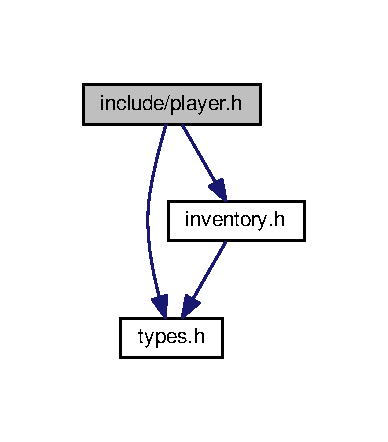
\includegraphics[width=186pt]{player_8h__incl}
\end{center}
\end{figure}
This graph shows which files directly or indirectly include this file\+:\nopagebreak
\begin{figure}[H]
\begin{center}
\leavevmode
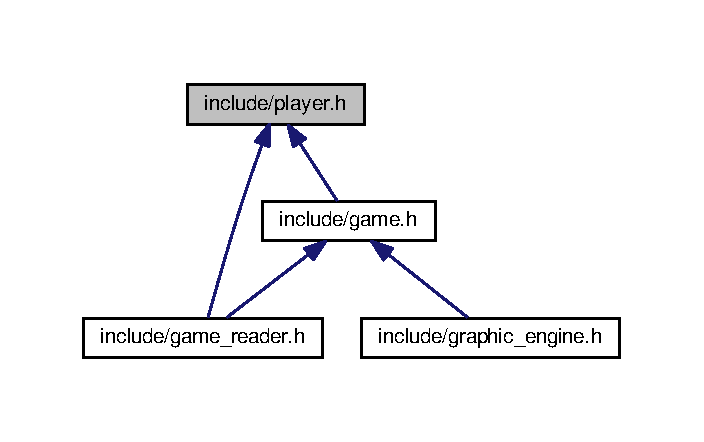
\includegraphics[width=338pt]{player_8h__dep__incl}
\end{center}
\end{figure}
\subsection*{Typedefs}
\begin{DoxyCompactItemize}
\item 
typedef struct \+\_\+\+Player \hyperlink{player_8h_af30e2030635a69690f85e48bc6ef202f}{Player}\hypertarget{player_8h_af30e2030635a69690f85e48bc6ef202f}{}\label{player_8h_af30e2030635a69690f85e48bc6ef202f}

\begin{DoxyCompactList}\small\item\em It holds the necessary data to manage a player. \end{DoxyCompactList}\end{DoxyCompactItemize}
\subsection*{Functions}
\begin{Indent}{\bf player\+\_\+create}\par
{\em It creates a player with the id passed.

\begin{DoxyAuthor}{Author}
Victor Yrazusta, edited by Alejandro Pascual 
\end{DoxyAuthor}
\begin{DoxyVersion}{Version}
1.\+0 
\end{DoxyVersion}
\begin{DoxyDate}{Date}
19-\/02-\/2018 
\end{DoxyDate}

\begin{DoxyParams}{Parameters}
{\em Id} & -\/$>$ the Id of the created player. \\
\hline
{\em int} & -\/$>$ which will define the size of the inventory of the player. \\
\hline
\end{DoxyParams}
\begin{DoxyReturn}{Returns}
A Player$\ast$, which points towards the created player. 
\end{DoxyReturn}
}\begin{DoxyCompactItemize}
\item 
\hyperlink{player_8h_af30e2030635a69690f85e48bc6ef202f}{Player} $\ast$ {\bfseries player\+\_\+create} (\hyperlink{types_8h_a845e604fb28f7e3d97549da3448149d3}{Id}, int inventory\+\_\+size)\hypertarget{player_8h_afbb8e3b390ae646cddff75ca6029272e}{}\label{player_8h_afbb8e3b390ae646cddff75ca6029272e}

\end{DoxyCompactItemize}
\end{Indent}
\begin{Indent}{\bf player\+\_\+destroy}\par
{\em It deallocates the memory reserved for the Player$\ast$ passed.

\begin{DoxyAuthor}{Author}
Alejandro Pascual 
\end{DoxyAuthor}
\begin{DoxyVersion}{Version}
1.\+0 
\end{DoxyVersion}
\begin{DoxyDate}{Date}
19-\/02-\/2018 
\end{DoxyDate}

\begin{DoxyParams}{Parameters}
{\em Player$\ast$} & -\/$>$ a player which will be deallocated. \\
\hline
\end{DoxyParams}
\begin{DoxyReturn}{Returns}
A S\+T\+A\+T\+US, which could be E\+R\+R\+OR if the pointer passed as an argument is N\+U\+LL, or OK otherwise. 
\end{DoxyReturn}
}\begin{DoxyCompactItemize}
\item 
\hyperlink{types_8h_a32c27cc471df37f4fc818d65de0a56c4}{S\+T\+A\+T\+US} {\bfseries player\+\_\+destroy} (\hyperlink{player_8h_af30e2030635a69690f85e48bc6ef202f}{Player} $\ast$)\hypertarget{player_8h_a7b6d052be93fe0c1b765e2a1f15baaee}{}\label{player_8h_a7b6d052be93fe0c1b765e2a1f15baaee}

\end{DoxyCompactItemize}
\end{Indent}
\begin{Indent}{\bf player\+\_\+set\+\_\+name}\par
{\em It changes the name of the passed player to the passed name.

\begin{DoxyAuthor}{Author}
Victor Yrazusta 
\end{DoxyAuthor}
\begin{DoxyVersion}{Version}
1.\+0 
\end{DoxyVersion}
\begin{DoxyDate}{Date}
19-\/02-\/2018 
\end{DoxyDate}

\begin{DoxyParams}{Parameters}
{\em Player$\ast$} & -\/$>$ a player whose name will be changed. \\
\hline
{\em char$\ast$} & -\/$>$ a string with the new name for the player. \\
\hline
\end{DoxyParams}
\begin{DoxyReturn}{Returns}
A S\+T\+A\+T\+US, which could be \char`\"{}\+E\+R\+R\+O\+R\char`\"{} if the pointer passed as an argument is N\+U\+LL, or \char`\"{}\+O\+K\char`\"{} otherwise. 
\end{DoxyReturn}
}\begin{DoxyCompactItemize}
\item 
\hyperlink{types_8h_a32c27cc471df37f4fc818d65de0a56c4}{S\+T\+A\+T\+US} {\bfseries player\+\_\+set\+\_\+name} (\hyperlink{player_8h_af30e2030635a69690f85e48bc6ef202f}{Player} $\ast$, char $\ast$name)\hypertarget{player_8h_a4398dd9b34eeb7aea457014ac06475fb}{}\label{player_8h_a4398dd9b34eeb7aea457014ac06475fb}

\end{DoxyCompactItemize}
\end{Indent}
\begin{Indent}{\bf player\+\_\+set\+\_\+graphic\+\_\+description}\par
{\em It changes the graphic\+\_\+description of the passed player to the passed graphic\+\_\+description.

\begin{DoxyAuthor}{Author}
Eric Morales 
\end{DoxyAuthor}
\begin{DoxyVersion}{Version}
1.\+0 
\end{DoxyVersion}
\begin{DoxyDate}{Date}
04-\/04-\/2018 
\end{DoxyDate}

\begin{DoxyParams}{Parameters}
{\em Player$\ast$} & -\/$>$ the player whose graphic\+\_\+description will be changed. \\
\hline
{\em char$\ast$} & -\/$>$ a string with the new graphic\+\_\+description for the player. \\
\hline
\end{DoxyParams}
\begin{DoxyReturn}{Returns}
A S\+T\+A\+T\+US, which could be \char`\"{}\+E\+R\+R\+O\+R\char`\"{} if the pointer passed as an argument is N\+U\+LL, or \char`\"{}\+O\+K\char`\"{} otherwise. 
\end{DoxyReturn}
}\begin{DoxyCompactItemize}
\item 
\hyperlink{types_8h_a32c27cc471df37f4fc818d65de0a56c4}{S\+T\+A\+T\+US} {\bfseries player\+\_\+set\+\_\+graphic\+\_\+description} (\hyperlink{player_8h_af30e2030635a69690f85e48bc6ef202f}{Player} $\ast$, char $\ast$graphic\+\_\+description)\hypertarget{player_8h_a3ffbf18e583964ec57e0916d272bc134}{}\label{player_8h_a3ffbf18e583964ec57e0916d272bc134}

\end{DoxyCompactItemize}
\end{Indent}
\begin{Indent}{\bf object\+\_\+set\+\_\+location}\par
{\em It changes the location of the passed player to the passed id of the new location.

\begin{DoxyAuthor}{Author}
V�ctor Yrazusta 
\end{DoxyAuthor}
\begin{DoxyVersion}{Version}
1.\+0 
\end{DoxyVersion}
\begin{DoxyDate}{Date}
19-\/02-\/2018 
\end{DoxyDate}

\begin{DoxyParams}{Parameters}
{\em Player$\ast$} & -\/$>$ the player whose location will be changed. \\
\hline
{\em Id} & -\/$>$ the new location for the player. \\
\hline
\end{DoxyParams}
\begin{DoxyReturn}{Returns}
A S\+T\+A\+T\+US, which could be \char`\"{}\+E\+R\+R\+O\+R\char`\"{} if the pointer passed as an argument is N\+U\+LL, or \char`\"{}\+O\+K\char`\"{} otherwise. 
\end{DoxyReturn}
}\begin{DoxyCompactItemize}
\item 
\hyperlink{types_8h_a32c27cc471df37f4fc818d65de0a56c4}{S\+T\+A\+T\+US} {\bfseries player\+\_\+set\+\_\+location} (\hyperlink{player_8h_af30e2030635a69690f85e48bc6ef202f}{Player} $\ast$, \hyperlink{types_8h_a845e604fb28f7e3d97549da3448149d3}{Id} location)\hypertarget{player_8h_a89c140a37db2ff01961fd4cde1fde6ff}{}\label{player_8h_a89c140a37db2ff01961fd4cde1fde6ff}

\end{DoxyCompactItemize}
\end{Indent}
\begin{Indent}{\bf object\+\_\+add\+\_\+object}\par
{\em It adds the object id to the set of the inventory of the player.

\begin{DoxyAuthor}{Author}
Alejandro Pascual 
\end{DoxyAuthor}
\begin{DoxyVersion}{Version}
2.\+0 
\end{DoxyVersion}
\begin{DoxyDate}{Date}
19-\/02-\/2018 
\end{DoxyDate}

\begin{DoxyParams}{Parameters}
{\em Player$\ast$} & -\/$>$ the player whose inventory will be modified \\
\hline
{\em Id} & -\/$>$ the (object) id that will be added to the set. \\
\hline
\end{DoxyParams}
\begin{DoxyReturn}{Returns}
A S\+T\+A\+T\+US, which could be \char`\"{}\+E\+R\+R\+O\+R\char`\"{} if the pointer passed as an argument is N\+U\+LL, or \char`\"{}\+O\+K\char`\"{} otherwise. 
\end{DoxyReturn}
}\begin{DoxyCompactItemize}
\item 
\hyperlink{types_8h_a32c27cc471df37f4fc818d65de0a56c4}{S\+T\+A\+T\+US} {\bfseries player\+\_\+add\+\_\+object} (\hyperlink{player_8h_af30e2030635a69690f85e48bc6ef202f}{Player} $\ast$, \hyperlink{types_8h_a845e604fb28f7e3d97549da3448149d3}{Id} object\+\_\+id)\hypertarget{player_8h_aac23ee8c4fb5c0f267ab9bc4558740c0}{}\label{player_8h_aac23ee8c4fb5c0f267ab9bc4558740c0}

\end{DoxyCompactItemize}
\end{Indent}
\begin{Indent}{\bf object\+\_\+del\+\_\+object}\par
{\em It removes the object id from the set of the inventory of the player.

\begin{DoxyAuthor}{Author}
Alejandro Pascual 
\end{DoxyAuthor}
\begin{DoxyVersion}{Version}
1.\+0 
\end{DoxyVersion}
\begin{DoxyDate}{Date}
19-\/02-\/2018 
\end{DoxyDate}

\begin{DoxyParams}{Parameters}
{\em Player$\ast$} & -\/$>$ a player whose inventory will be modified. \\
\hline
{\em Id} & -\/$>$ the (object) id that will be removed from the set. \\
\hline
\end{DoxyParams}
\begin{DoxyReturn}{Returns}
A S\+T\+A\+T\+US, which could be \char`\"{}\+E\+R\+R\+O\+R\char`\"{} if the pointer passed as an argument is N\+U\+LL, or \char`\"{}\+O\+K\char`\"{} otherwise. 
\end{DoxyReturn}
}\begin{DoxyCompactItemize}
\item 
\hyperlink{types_8h_a32c27cc471df37f4fc818d65de0a56c4}{S\+T\+A\+T\+US} {\bfseries player\+\_\+del\+\_\+object} (\hyperlink{player_8h_af30e2030635a69690f85e48bc6ef202f}{Player} $\ast$, \hyperlink{types_8h_a845e604fb28f7e3d97549da3448149d3}{Id} object\+\_\+id)\hypertarget{player_8h_af1504b6bfab73afb5fe341d0d6af03df}{}\label{player_8h_af1504b6bfab73afb5fe341d0d6af03df}

\end{DoxyCompactItemize}
\end{Indent}
\begin{Indent}{\bf player\+\_\+get\+\_\+name}\par
{\em It returns the name of the player passed as an argument.

\begin{DoxyAuthor}{Author}
Victor Yrazusta 
\end{DoxyAuthor}
\begin{DoxyVersion}{Version}
1.\+0 
\end{DoxyVersion}
\begin{DoxyDate}{Date}
19-\/02-\/2018 
\end{DoxyDate}

\begin{DoxyParams}{Parameters}
{\em Player$\ast$} & -\/$>$ the player whose name will be returned. \\
\hline
\end{DoxyParams}
\begin{DoxyReturn}{Returns}
A const char$\ast$, which could be N\+U\+LL if the pointer passed as an argument is N\+U\+LL, or the player\textquotesingle{}s name otherwise. 
\end{DoxyReturn}
}\begin{DoxyCompactItemize}
\item 
const char $\ast$ {\bfseries player\+\_\+get\+\_\+name} (\hyperlink{player_8h_af30e2030635a69690f85e48bc6ef202f}{Player} $\ast$)\hypertarget{player_8h_a49d3f1d3881efbab6d6db1920866c3ab}{}\label{player_8h_a49d3f1d3881efbab6d6db1920866c3ab}

\end{DoxyCompactItemize}
\end{Indent}
\begin{Indent}{\bf player\+\_\+get\+\_\+graphic\+\_\+description}\par
{\em It returns the graphic\+\_\+description of the player passed as an argument.

\begin{DoxyAuthor}{Author}
Eric Morales 
\end{DoxyAuthor}
\begin{DoxyVersion}{Version}
1.\+0 
\end{DoxyVersion}
\begin{DoxyDate}{Date}
04-\/04-\/2018 
\end{DoxyDate}

\begin{DoxyParams}{Parameters}
{\em Player$\ast$} & -\/$>$ the player whose graphic\+\_\+description will be returned. \\
\hline
\end{DoxyParams}
\begin{DoxyReturn}{Returns}
A const char$\ast$, which could be N\+U\+LL if the pointer passed as an argument is N\+U\+LL, or the player\textquotesingle{}s graphic\+\_\+description otherwise. 
\end{DoxyReturn}
}\begin{DoxyCompactItemize}
\item 
const char $\ast$ {\bfseries player\+\_\+get\+\_\+graphic\+\_\+description} (\hyperlink{player_8h_af30e2030635a69690f85e48bc6ef202f}{Player} $\ast$)\hypertarget{player_8h_a82cc551b77170a7156d74e4525a82701}{}\label{player_8h_a82cc551b77170a7156d74e4525a82701}

\end{DoxyCompactItemize}
\end{Indent}
\begin{Indent}{\bf object\+\_\+get\+\_\+id}\par
{\em It returns the id of the player passed as an argument.

\begin{DoxyAuthor}{Author}
Alejandro Pascual 
\end{DoxyAuthor}
\begin{DoxyVersion}{Version}
1.\+0 
\end{DoxyVersion}
\begin{DoxyDate}{Date}
19-\/02-\/2018 
\end{DoxyDate}

\begin{DoxyParams}{Parameters}
{\em Player$\ast$} & -\/$>$ the player whose id will be returned. \\
\hline
\end{DoxyParams}
\begin{DoxyReturn}{Returns}
An Id, which could be N\+O\+\_\+\+ID if the pointer passed as an argument is N\+U\+LL, or the player\textquotesingle{}s id otherwise. 
\end{DoxyReturn}
}\begin{DoxyCompactItemize}
\item 
\hyperlink{types_8h_a845e604fb28f7e3d97549da3448149d3}{Id} {\bfseries player\+\_\+get\+\_\+id} (\hyperlink{player_8h_af30e2030635a69690f85e48bc6ef202f}{Player} $\ast$)\hypertarget{player_8h_a59ac73ab3cc7d0c888d44bfcf96c6551}{}\label{player_8h_a59ac73ab3cc7d0c888d44bfcf96c6551}

\end{DoxyCompactItemize}
\end{Indent}
\begin{Indent}{\bf player\+\_\+get\+\_\+location}\par
{\em It returns the id of the location of the player passed as an argument.

\begin{DoxyAuthor}{Author}
V�ctor Yrazusta 
\end{DoxyAuthor}
\begin{DoxyVersion}{Version}
1.\+0 
\end{DoxyVersion}
\begin{DoxyDate}{Date}
19-\/02-\/2018 
\end{DoxyDate}

\begin{DoxyParams}{Parameters}
{\em Player$\ast$} & -\/$>$ the player whose location id will be returned. \\
\hline
\end{DoxyParams}
\begin{DoxyReturn}{Returns}
The Id, which could be N\+O\+\_\+\+ID if the pointer passed as an argument is N\+U\+LL, of the player\textquotesingle{}s location id otherwise. 
\end{DoxyReturn}
}\begin{DoxyCompactItemize}
\item 
\hyperlink{types_8h_a845e604fb28f7e3d97549da3448149d3}{Id} {\bfseries player\+\_\+get\+\_\+location} (\hyperlink{player_8h_af30e2030635a69690f85e48bc6ef202f}{Player} $\ast$)\hypertarget{player_8h_aa0c1b8174545f2675392702307cde9bb}{}\label{player_8h_aa0c1b8174545f2675392702307cde9bb}

\end{DoxyCompactItemize}
\end{Indent}
\begin{Indent}{\bf player\+\_\+get\+\_\+objects\+\_\+number}\par
{\em It returns the current number of objects in the inventory of the player.

\begin{DoxyAuthor}{Author}
Alejandro Pascual 
\end{DoxyAuthor}
\begin{DoxyVersion}{Version}
1.\+0 
\end{DoxyVersion}
\begin{DoxyDate}{Date}
01-\/04-\/2018 
\end{DoxyDate}

\begin{DoxyParams}{Parameters}
{\em Player$\ast$} & -\/$>$ the player from which we will get the number of objects. \\
\hline
\end{DoxyParams}
\begin{DoxyReturn}{Returns}
An int, which is the current number of objects in the inventory of the player. 
\end{DoxyReturn}
}\begin{DoxyCompactItemize}
\item 
int {\bfseries player\+\_\+get\+\_\+objects\+\_\+number} (\hyperlink{player_8h_af30e2030635a69690f85e48bc6ef202f}{Player} $\ast$)\hypertarget{player_8h_ac6b2ae036b35cb6abde5af65a278d515}{}\label{player_8h_ac6b2ae036b35cb6abde5af65a278d515}

\end{DoxyCompactItemize}
\end{Indent}
\begin{Indent}{\bf player\+\_\+get\+\_\+max\+\_\+objects}\par
{\em It returns the capacity of the Inventory of the Player.

\begin{DoxyAuthor}{Author}
Alejandro Pascual 
\end{DoxyAuthor}
\begin{DoxyVersion}{Version}
1.\+0 
\end{DoxyVersion}
\begin{DoxyDate}{Date}
01-\/04-\/2018 
\end{DoxyDate}

\begin{DoxyParams}{Parameters}
{\em Player$\ast$} & -\/$>$ a player from which we will get the maximum number of objects. \\
\hline
\end{DoxyParams}
\begin{DoxyReturn}{Returns}
An int, which is the capacity of the Inventory of the Player and 0 if the Player or the Inventory are N\+U\+LL. 
\end{DoxyReturn}
}\begin{DoxyCompactItemize}
\item 
int {\bfseries player\+\_\+get\+\_\+max\+\_\+objects} (\hyperlink{player_8h_af30e2030635a69690f85e48bc6ef202f}{Player} $\ast$)\hypertarget{player_8h_aec0055239578db4ed7789444ecb780b8}{}\label{player_8h_aec0055239578db4ed7789444ecb780b8}

\end{DoxyCompactItemize}
\end{Indent}
\begin{Indent}{\bf player\+\_\+get\+\_\+object}\par
{\em It returns the id of the object in the postion specified on the set of the inventory of the player.

\begin{DoxyAuthor}{Author}
Alejandro Pascual 
\end{DoxyAuthor}
\begin{DoxyVersion}{Version}
1.\+0 
\end{DoxyVersion}
\begin{DoxyDate}{Date}
01-\/04-\/2018 
\end{DoxyDate}

\begin{DoxyParams}{Parameters}
{\em Player$\ast$} & -\/$>$ the player which we will get the object from. \\
\hline
{\em int} & -\/$>$ an integer that specifies the postion in the set. \\
\hline
\end{DoxyParams}
\begin{DoxyReturn}{Returns}
The Id, which could be N\+O\+\_\+\+ID if the pointer passed as an argument is N\+U\+LL, of the object in the specified position on the set. 
\end{DoxyReturn}
}\begin{DoxyCompactItemize}
\item 
\hyperlink{types_8h_a845e604fb28f7e3d97549da3448149d3}{Id} {\bfseries player\+\_\+get\+\_\+object} (\hyperlink{player_8h_af30e2030635a69690f85e48bc6ef202f}{Player} $\ast$, int position)\hypertarget{player_8h_aff5e36d144f93cde5c574508a7cb184c}{}\label{player_8h_aff5e36d144f93cde5c574508a7cb184c}

\end{DoxyCompactItemize}
\end{Indent}
\begin{Indent}{\bf player\+\_\+check\+\_\+object}\par
{\em It checks if the passed object\+\_\+id is in the set of the inventory of the player.

\begin{DoxyAuthor}{Author}
Alejandro Pascual 
\end{DoxyAuthor}
\begin{DoxyVersion}{Version}
1.\+0 
\end{DoxyVersion}
\begin{DoxyDate}{Date}
03-\/04-\/2018 
\end{DoxyDate}

\begin{DoxyParams}{Parameters}
{\em Player$\ast$} & -\/$>$ the player whose inventory will be checked seaching the object. \\
\hline
{\em Id} & -\/$>$ the id of the object to be checked. \\
\hline
\end{DoxyParams}
\begin{DoxyReturn}{Returns}
A Bool, which is true if passed object id is in the set of the inventory of the player. 
\end{DoxyReturn}
}\begin{DoxyCompactItemize}
\item 
\hyperlink{types_8h_a3e5b8192e7d9ffaf3542f1210aec18dd}{B\+O\+OL} {\bfseries player\+\_\+check\+\_\+object} (\hyperlink{player_8h_af30e2030635a69690f85e48bc6ef202f}{Player} $\ast$, \hyperlink{types_8h_a845e604fb28f7e3d97549da3448149d3}{Id} object\+\_\+id)\hypertarget{player_8h_a10fb2fe31cd9ee4015039581fcfa8e9e}{}\label{player_8h_a10fb2fe31cd9ee4015039581fcfa8e9e}

\end{DoxyCompactItemize}
\end{Indent}
\begin{Indent}{\bf player\+\_\+is\+\_\+empty}\par
{\em This function is used to check if the inventory of player is empty.

\begin{DoxyAuthor}{Author}
Alejandro Pascual 
\end{DoxyAuthor}
\begin{DoxyVersion}{Version}
1.\+0 
\end{DoxyVersion}
\begin{DoxyDate}{Date}
31-\/03-\/2018 
\end{DoxyDate}

\begin{DoxyParams}{Parameters}
{\em Player$\ast$} & -\/$>$ a player whose inventory will be checked. \\
\hline
\end{DoxyParams}
\begin{DoxyReturn}{Returns}
A Bool, which is true if the inventory of the player is empty or if the player is N\+U\+LL. 
\end{DoxyReturn}
}\begin{DoxyCompactItemize}
\item 
\hyperlink{types_8h_a3e5b8192e7d9ffaf3542f1210aec18dd}{B\+O\+OL} {\bfseries player\+\_\+is\+\_\+empty} (\hyperlink{player_8h_af30e2030635a69690f85e48bc6ef202f}{Player} $\ast$)\hypertarget{player_8h_a79ebe803137e5d8621feb46595ee58db}{}\label{player_8h_a79ebe803137e5d8621feb46595ee58db}

\end{DoxyCompactItemize}
\end{Indent}
\begin{Indent}{\bf player\+\_\+is\+\_\+full}\par
{\em This function is used to check if the inventory of player is full.

\begin{DoxyAuthor}{Author}
Alejandro Pascual 
\end{DoxyAuthor}
\begin{DoxyVersion}{Version}
1.\+0 
\end{DoxyVersion}
\begin{DoxyDate}{Date}
31-\/03-\/2018 
\end{DoxyDate}

\begin{DoxyParams}{Parameters}
{\em Player$\ast$} & -\/$>$ whose inventory will be checked. \\
\hline
\end{DoxyParams}
\begin{DoxyReturn}{Returns}
A Bool, which is true if the inventory of the player is full or if the player is N\+U\+LL. 
\end{DoxyReturn}
}\begin{DoxyCompactItemize}
\item 
\hyperlink{types_8h_a3e5b8192e7d9ffaf3542f1210aec18dd}{B\+O\+OL} {\bfseries player\+\_\+is\+\_\+full} (\hyperlink{player_8h_af30e2030635a69690f85e48bc6ef202f}{Player} $\ast$)\hypertarget{player_8h_a717d470f9c93469ea00c97fbd058d77a}{}\label{player_8h_a717d470f9c93469ea00c97fbd058d77a}

\end{DoxyCompactItemize}
\end{Indent}
\begin{Indent}{\bf player\+\_\+print}\par
{\em It prints on the standard output the values of the player passed as an argument.

\begin{DoxyAuthor}{Author}
Victor Yrazusta 
\end{DoxyAuthor}
\begin{DoxyVersion}{Version}
1.\+0 
\end{DoxyVersion}
\begin{DoxyDate}{Date}
19-\/02-\/2018 
\end{DoxyDate}

\begin{DoxyParams}{Parameters}
{\em Player$\ast$} & -\/$>$ whose data will be printed. \\
\hline
\end{DoxyParams}
\begin{DoxyReturn}{Returns}
A S\+T\+A\+T\+US, which could be \char`\"{}\+E\+R\+R\+O\+R\char`\"{} if the pointer passed as an argument is N\+U\+LL, or \char`\"{}\+O\+K\char`\"{} otherwise.
\end{DoxyReturn}
N\+O\+TE\+: This function was created for debugging purposes only and it is not used in the normal execution of the game. }\begin{DoxyCompactItemize}
\item 
\hyperlink{types_8h_a32c27cc471df37f4fc818d65de0a56c4}{S\+T\+A\+T\+US} {\bfseries player\+\_\+print} (\hyperlink{player_8h_af30e2030635a69690f85e48bc6ef202f}{Player} $\ast$)\hypertarget{player_8h_afc71635a7e93ea286e80a82a8500b23b}{}\label{player_8h_afc71635a7e93ea286e80a82a8500b23b}

\end{DoxyCompactItemize}
\end{Indent}


\subsection{Detailed Description}
It defines a player and the necessary functions to work with it. 

\begin{DoxyAuthor}{Author}
Alejandro Pascual and Victor Yrazusta 
\end{DoxyAuthor}
\begin{DoxyVersion}{Version}
1.\+0 
\end{DoxyVersion}
\begin{DoxyDate}{Date}
13-\/02-\/2018 
\end{DoxyDate}
\begin{DoxyCopyright}{Copyright}
G\+NU Public License 
\end{DoxyCopyright}

\hypertarget{player__test_8h}{}\section{include/player\+\_\+test.h File Reference}
\label{player__test_8h}\index{include/player\+\_\+test.\+h@{include/player\+\_\+test.\+h}}


It declares the tests for the player module.  


\subsection*{Functions}
\begin{DoxyCompactItemize}
\item 
void \hyperlink{player__test_8h_ab29768452373e16bb6aaa1f7998f62fb}{test1\+\_\+player\+\_\+create} ()
\item 
void \hyperlink{player__test_8h_a4f6eca5f9d8c08d2a7fc70c209ecf854}{test2\+\_\+player\+\_\+create} ()
\item 
void \hyperlink{player__test_8h_a9d87c09e6af910d695265e3fd77ae3a2}{test1\+\_\+player\+\_\+set\+\_\+name} ()
\item 
void \hyperlink{player__test_8h_a6e7ce8ff791f4bf63749df647a44263f}{test2\+\_\+player\+\_\+set\+\_\+name} ()
\item 
void \hyperlink{player__test_8h_a447ebbb4ba2206abeaf4b60200e312da}{test3\+\_\+player\+\_\+set\+\_\+name} ()
\item 
void \hyperlink{player__test_8h_adfd8f1d4fd7d500f9b5236db4e697ea3}{test1\+\_\+player\+\_\+set\+\_\+graphic\+\_\+description} ()
\item 
void \hyperlink{player__test_8h_a4d18de1dc3a06db35a47aaa2c81df4fd}{test2\+\_\+player\+\_\+set\+\_\+graphic\+\_\+description} ()
\item 
void \hyperlink{player__test_8h_a7f865b46cfa086222fe0bfd1b9ed97f7}{test3\+\_\+player\+\_\+set\+\_\+graphic\+\_\+description} ()
\item 
void \hyperlink{player__test_8h_aec6799a4f46c3f3c471fcb668addcad4}{test1\+\_\+player\+\_\+set\+\_\+location} ()
\item 
void \hyperlink{player__test_8h_a2c702753d9e2e3df9ef4abf2d1b9bc8d}{test2\+\_\+player\+\_\+set\+\_\+location} ()
\item 
void \hyperlink{player__test_8h_a317c0c84ef6ef843c15d5bab4a6b8a38}{test3\+\_\+player\+\_\+set\+\_\+location} ()
\item 
void \hyperlink{player__test_8h_a94068667d8faa66a4ad293dd2c60f2ef}{test1\+\_\+player\+\_\+get\+\_\+name} ()
\item 
void \hyperlink{player__test_8h_a3aa908fd360b74e7786422260e8e16a0}{test2\+\_\+player\+\_\+get\+\_\+name} ()
\item 
void \hyperlink{player__test_8h_a790a75dc179c00c60c784d3e34c0e5aa}{test1\+\_\+player\+\_\+get\+\_\+id} ()
\item 
void \hyperlink{player__test_8h_a9fa80f0c0e46b45eb9f1685b102a5826}{test2\+\_\+player\+\_\+get\+\_\+id} ()
\item 
void \hyperlink{player__test_8h_a07beea3b974453e5d8001d04e6db5ac4}{test1\+\_\+player\+\_\+get\+\_\+graphic\+\_\+description} ()
\item 
void \hyperlink{player__test_8h_a94aa58d9c954a4817ea34ba7d7c17493}{test2\+\_\+player\+\_\+get\+\_\+graphic\+\_\+description} ()
\item 
void \hyperlink{player__test_8h_a53eb6ee101f01fe988c5da03129d2e2f}{test1\+\_\+player\+\_\+get\+\_\+object} ()
\item 
void \hyperlink{player__test_8h_a83e8fea42cd87151cd67d0643a78134f}{test2\+\_\+player\+\_\+get\+\_\+object} ()
\item 
void \hyperlink{player__test_8h_af1b1a4517ec347b3b953c9fc9b3ea1a5}{test1\+\_\+player\+\_\+get\+\_\+objects\+\_\+number} ()
\item 
void \hyperlink{player__test_8h_a718933fd0429cdc840c6624882550d3b}{test2\+\_\+player\+\_\+get\+\_\+objects\+\_\+number} ()
\item 
void \hyperlink{player__test_8h_a61bbeaff50cc839f226a53ed9b808784}{test3\+\_\+player\+\_\+get\+\_\+objects\+\_\+number} ()
\item 
void \hyperlink{player__test_8h_aa3a3053dd61cc8d45d019aa37e9f1379}{test4\+\_\+player\+\_\+get\+\_\+objects\+\_\+number} ()
\item 
void \hyperlink{player__test_8h_a408a557a0cff748c10fb9a03445af191}{test1\+\_\+player\+\_\+get\+\_\+location} ()
\item 
void \hyperlink{player__test_8h_a4c5605fac4bd716e1dfb2744db4fa8a1}{test2\+\_\+player\+\_\+get\+\_\+location} ()
\item 
void \hyperlink{player__test_8h_a14a3e4867e2ad3287c8efa99cd36904e}{test1\+\_\+player\+\_\+add\+\_\+object} ()
\item 
void \hyperlink{player__test_8h_a864d3935cf61953950b10df0e656306d}{test2\+\_\+player\+\_\+add\+\_\+object} ()
\item 
void \hyperlink{player__test_8h_ab8680555a9d30950ffa0547011a0f787}{test1\+\_\+player\+\_\+del\+\_\+object} ()
\item 
void \hyperlink{player__test_8h_a32008cea3e74553151b6c8c8ad1b565a}{test2\+\_\+player\+\_\+del\+\_\+object} ()
\item 
void \hyperlink{player__test_8h_a452322fef33fc8706043c5067352eccd}{test3\+\_\+player\+\_\+del\+\_\+object} ()
\item 
void \hyperlink{player__test_8h_a9e7594fd2a1016abea94e0b88016d6ec}{test1\+\_\+player\+\_\+is\+\_\+empty} ()
\item 
void \hyperlink{player__test_8h_ab101e35e3034e348688b0a8ffd81f8ad}{test2\+\_\+player\+\_\+is\+\_\+empty} ()
\item 
void \hyperlink{player__test_8h_a08b329fb04b5d2a9023492e00bd19e48}{test3\+\_\+player\+\_\+is\+\_\+empty} ()
\item 
void \hyperlink{player__test_8h_a2c7a96147ce996da70dce4b4cb37ecef}{test1\+\_\+player\+\_\+is\+\_\+full} ()
\item 
void \hyperlink{player__test_8h_a2a0781d2fbfb7f0d8870b7501db230a6}{test2\+\_\+player\+\_\+is\+\_\+full} ()
\item 
void \hyperlink{player__test_8h_a8260b22f8889de8693acc075136697f3}{test3\+\_\+player\+\_\+is\+\_\+full} ()
\item 
void \hyperlink{player__test_8h_a96dcde9701d8318c454b634c13969503}{test4\+\_\+player\+\_\+is\+\_\+full} ()
\item 
void \hyperlink{player__test_8h_a95396b550249d790fe55be1e553517ae}{test1\+\_\+player\+\_\+check\+\_\+object} ()
\item 
void \hyperlink{player__test_8h_a18d23e4d24cc31a552f264e270856a49}{test2\+\_\+player\+\_\+check\+\_\+object} ()
\item 
void \hyperlink{player__test_8h_a874f5bf56d0cca218979fee114a90d22}{test3\+\_\+player\+\_\+check\+\_\+object} ()
\end{DoxyCompactItemize}


\subsection{Detailed Description}
It declares the tests for the player module. 

\begin{DoxyAuthor}{Author}
Eric Morales 
\end{DoxyAuthor}
\begin{DoxyVersion}{Version}
1.\+0 
\end{DoxyVersion}
\begin{DoxyDate}{Date}
08-\/04-\/2018 
\end{DoxyDate}
\begin{DoxyCopyright}{Copyright}
G\+NU Public License 
\end{DoxyCopyright}


\subsection{Function Documentation}
\index{player\+\_\+test.\+h@{player\+\_\+test.\+h}!test1\+\_\+player\+\_\+add\+\_\+object@{test1\+\_\+player\+\_\+add\+\_\+object}}
\index{test1\+\_\+player\+\_\+add\+\_\+object@{test1\+\_\+player\+\_\+add\+\_\+object}!player\+\_\+test.\+h@{player\+\_\+test.\+h}}
\subsubsection[{\texorpdfstring{test1\+\_\+player\+\_\+add\+\_\+object()}{test1_player_add_object()}}]{\setlength{\rightskip}{0pt plus 5cm}void test1\+\_\+player\+\_\+add\+\_\+object (
\begin{DoxyParamCaption}
{}
\end{DoxyParamCaption}
)}\hypertarget{player__test_8h_a14a3e4867e2ad3287c8efa99cd36904e}{}\label{player__test_8h_a14a3e4867e2ad3287c8efa99cd36904e}
\begin{DoxyRefDesc}{Test}
\item[\hyperlink{test__test000197}{Test}]Test if objects are added properly onto the player \end{DoxyRefDesc}
\begin{DoxyPrecond}{Precondition}
Created player and object Id 
\end{DoxyPrecond}
\begin{DoxyPostcond}{Postcondition}
O\+U\+T\+P\+UT==OK 
\end{DoxyPostcond}
\index{player\+\_\+test.\+h@{player\+\_\+test.\+h}!test1\+\_\+player\+\_\+check\+\_\+object@{test1\+\_\+player\+\_\+check\+\_\+object}}
\index{test1\+\_\+player\+\_\+check\+\_\+object@{test1\+\_\+player\+\_\+check\+\_\+object}!player\+\_\+test.\+h@{player\+\_\+test.\+h}}
\subsubsection[{\texorpdfstring{test1\+\_\+player\+\_\+check\+\_\+object()}{test1_player_check_object()}}]{\setlength{\rightskip}{0pt plus 5cm}void test1\+\_\+player\+\_\+check\+\_\+object (
\begin{DoxyParamCaption}
{}
\end{DoxyParamCaption}
)}\hypertarget{player__test_8h_a95396b550249d790fe55be1e553517ae}{}\label{player__test_8h_a95396b550249d790fe55be1e553517ae}
\begin{DoxyRefDesc}{Test}
\item[\hyperlink{test__test000209}{Test}]Test to see if the check object works on a Player with an object \end{DoxyRefDesc}
\begin{DoxyPrecond}{Precondition}
Player ID and Object Id 
\end{DoxyPrecond}
\begin{DoxyPostcond}{Postcondition}
O\+U\+T\+P\+UT==T\+R\+UE 
\end{DoxyPostcond}
\index{player\+\_\+test.\+h@{player\+\_\+test.\+h}!test1\+\_\+player\+\_\+create@{test1\+\_\+player\+\_\+create}}
\index{test1\+\_\+player\+\_\+create@{test1\+\_\+player\+\_\+create}!player\+\_\+test.\+h@{player\+\_\+test.\+h}}
\subsubsection[{\texorpdfstring{test1\+\_\+player\+\_\+create()}{test1_player_create()}}]{\setlength{\rightskip}{0pt plus 5cm}void test1\+\_\+player\+\_\+create (
\begin{DoxyParamCaption}
{}
\end{DoxyParamCaption}
)}\hypertarget{player__test_8h_ab29768452373e16bb6aaa1f7998f62fb}{}\label{player__test_8h_ab29768452373e16bb6aaa1f7998f62fb}
\begin{DoxyRefDesc}{Test}
\item[\hyperlink{test__test000172}{Test}]Test player creation \end{DoxyRefDesc}
\begin{DoxyPrecond}{Precondition}
Player Id and inventory size 
\end{DoxyPrecond}
\begin{DoxyPostcond}{Postcondition}
Non N\+U\+LL pointer to player 
\end{DoxyPostcond}
\index{player\+\_\+test.\+h@{player\+\_\+test.\+h}!test1\+\_\+player\+\_\+del\+\_\+object@{test1\+\_\+player\+\_\+del\+\_\+object}}
\index{test1\+\_\+player\+\_\+del\+\_\+object@{test1\+\_\+player\+\_\+del\+\_\+object}!player\+\_\+test.\+h@{player\+\_\+test.\+h}}
\subsubsection[{\texorpdfstring{test1\+\_\+player\+\_\+del\+\_\+object()}{test1_player_del_object()}}]{\setlength{\rightskip}{0pt plus 5cm}void test1\+\_\+player\+\_\+del\+\_\+object (
\begin{DoxyParamCaption}
{}
\end{DoxyParamCaption}
)}\hypertarget{player__test_8h_ab8680555a9d30950ffa0547011a0f787}{}\label{player__test_8h_ab8680555a9d30950ffa0547011a0f787}
\begin{DoxyRefDesc}{Test}
\item[\hyperlink{test__test000199}{Test}]Test if objects are deleted properly into the player \end{DoxyRefDesc}
\begin{DoxyPrecond}{Precondition}
Created player and object Id 
\end{DoxyPrecond}
\begin{DoxyPostcond}{Postcondition}
O\+U\+T\+P\+UT==OK 
\end{DoxyPostcond}
\index{player\+\_\+test.\+h@{player\+\_\+test.\+h}!test1\+\_\+player\+\_\+get\+\_\+graphic\+\_\+description@{test1\+\_\+player\+\_\+get\+\_\+graphic\+\_\+description}}
\index{test1\+\_\+player\+\_\+get\+\_\+graphic\+\_\+description@{test1\+\_\+player\+\_\+get\+\_\+graphic\+\_\+description}!player\+\_\+test.\+h@{player\+\_\+test.\+h}}
\subsubsection[{\texorpdfstring{test1\+\_\+player\+\_\+get\+\_\+graphic\+\_\+description()}{test1_player_get_graphic_description()}}]{\setlength{\rightskip}{0pt plus 5cm}void test1\+\_\+player\+\_\+get\+\_\+graphic\+\_\+description (
\begin{DoxyParamCaption}
{}
\end{DoxyParamCaption}
)}\hypertarget{player__test_8h_a07beea3b974453e5d8001d04e6db5ac4}{}\label{player__test_8h_a07beea3b974453e5d8001d04e6db5ac4}
\begin{DoxyRefDesc}{Test}
\item[\hyperlink{test__test000187}{Test}]Test to see if the created player with the given graphic description returns the given graphic description \end{DoxyRefDesc}
\begin{DoxyPrecond}{Precondition}
Player ID and a string with a graphic description 
\end{DoxyPrecond}
\begin{DoxyPostcond}{Postcondition}
O\+U\+T\+P\+UT==0 (equal strings) 
\end{DoxyPostcond}
\index{player\+\_\+test.\+h@{player\+\_\+test.\+h}!test1\+\_\+player\+\_\+get\+\_\+id@{test1\+\_\+player\+\_\+get\+\_\+id}}
\index{test1\+\_\+player\+\_\+get\+\_\+id@{test1\+\_\+player\+\_\+get\+\_\+id}!player\+\_\+test.\+h@{player\+\_\+test.\+h}}
\subsubsection[{\texorpdfstring{test1\+\_\+player\+\_\+get\+\_\+id()}{test1_player_get_id()}}]{\setlength{\rightskip}{0pt plus 5cm}void test1\+\_\+player\+\_\+get\+\_\+id (
\begin{DoxyParamCaption}
{}
\end{DoxyParamCaption}
)}\hypertarget{player__test_8h_a790a75dc179c00c60c784d3e34c0e5aa}{}\label{player__test_8h_a790a75dc179c00c60c784d3e34c0e5aa}
\begin{DoxyRefDesc}{Test}
\item[\hyperlink{test__test000185}{Test}]Test to see if Player has the given Id \end{DoxyRefDesc}
\begin{DoxyPrecond}{Precondition}
Player ID 
\end{DoxyPrecond}
\begin{DoxyPostcond}{Postcondition}
O\+U\+T\+P\+UT==OK 
\end{DoxyPostcond}
\index{player\+\_\+test.\+h@{player\+\_\+test.\+h}!test1\+\_\+player\+\_\+get\+\_\+location@{test1\+\_\+player\+\_\+get\+\_\+location}}
\index{test1\+\_\+player\+\_\+get\+\_\+location@{test1\+\_\+player\+\_\+get\+\_\+location}!player\+\_\+test.\+h@{player\+\_\+test.\+h}}
\subsubsection[{\texorpdfstring{test1\+\_\+player\+\_\+get\+\_\+location()}{test1_player_get_location()}}]{\setlength{\rightskip}{0pt plus 5cm}void test1\+\_\+player\+\_\+get\+\_\+location (
\begin{DoxyParamCaption}
{}
\end{DoxyParamCaption}
)}\hypertarget{player__test_8h_a408a557a0cff748c10fb9a03445af191}{}\label{player__test_8h_a408a557a0cff748c10fb9a03445af191}
\begin{DoxyRefDesc}{Test}
\item[\hyperlink{test__test000195}{Test}]Test if the location Id of the player is OK \end{DoxyRefDesc}
\begin{DoxyPrecond}{Precondition}
Created player and location Id 
\end{DoxyPrecond}
\begin{DoxyPostcond}{Postcondition}
O\+U\+T\+P\+UT==OK (matching Ids) 
\end{DoxyPostcond}
\index{player\+\_\+test.\+h@{player\+\_\+test.\+h}!test1\+\_\+player\+\_\+get\+\_\+name@{test1\+\_\+player\+\_\+get\+\_\+name}}
\index{test1\+\_\+player\+\_\+get\+\_\+name@{test1\+\_\+player\+\_\+get\+\_\+name}!player\+\_\+test.\+h@{player\+\_\+test.\+h}}
\subsubsection[{\texorpdfstring{test1\+\_\+player\+\_\+get\+\_\+name()}{test1_player_get_name()}}]{\setlength{\rightskip}{0pt plus 5cm}void test1\+\_\+player\+\_\+get\+\_\+name (
\begin{DoxyParamCaption}
{}
\end{DoxyParamCaption}
)}\hypertarget{player__test_8h_a94068667d8faa66a4ad293dd2c60f2ef}{}\label{player__test_8h_a94068667d8faa66a4ad293dd2c60f2ef}
\begin{DoxyRefDesc}{Test}
\item[\hyperlink{test__test000183}{Test}]Test to see if Player has the given name \end{DoxyRefDesc}
\begin{DoxyPrecond}{Precondition}
Player ID and a string with a name on it 
\end{DoxyPrecond}
\begin{DoxyPostcond}{Postcondition}
O\+U\+T\+P\+UT==0 (equal strings) 
\end{DoxyPostcond}
\index{player\+\_\+test.\+h@{player\+\_\+test.\+h}!test1\+\_\+player\+\_\+get\+\_\+object@{test1\+\_\+player\+\_\+get\+\_\+object}}
\index{test1\+\_\+player\+\_\+get\+\_\+object@{test1\+\_\+player\+\_\+get\+\_\+object}!player\+\_\+test.\+h@{player\+\_\+test.\+h}}
\subsubsection[{\texorpdfstring{test1\+\_\+player\+\_\+get\+\_\+object()}{test1_player_get_object()}}]{\setlength{\rightskip}{0pt plus 5cm}void test1\+\_\+player\+\_\+get\+\_\+object (
\begin{DoxyParamCaption}
{}
\end{DoxyParamCaption}
)}\hypertarget{player__test_8h_a53eb6ee101f01fe988c5da03129d2e2f}{}\label{player__test_8h_a53eb6ee101f01fe988c5da03129d2e2f}
\begin{DoxyRefDesc}{Test}
\item[\hyperlink{test__test000189}{Test}]Test to see if a Player has the given Object on its inventory. \end{DoxyRefDesc}
\begin{DoxyPrecond}{Precondition}
Player ID and Object Id 
\end{DoxyPrecond}
\begin{DoxyPostcond}{Postcondition}
O\+U\+T\+P\+UT==OK (matching Ids) 
\end{DoxyPostcond}
\index{player\+\_\+test.\+h@{player\+\_\+test.\+h}!test1\+\_\+player\+\_\+get\+\_\+objects\+\_\+number@{test1\+\_\+player\+\_\+get\+\_\+objects\+\_\+number}}
\index{test1\+\_\+player\+\_\+get\+\_\+objects\+\_\+number@{test1\+\_\+player\+\_\+get\+\_\+objects\+\_\+number}!player\+\_\+test.\+h@{player\+\_\+test.\+h}}
\subsubsection[{\texorpdfstring{test1\+\_\+player\+\_\+get\+\_\+objects\+\_\+number()}{test1_player_get_objects_number()}}]{\setlength{\rightskip}{0pt plus 5cm}void test1\+\_\+player\+\_\+get\+\_\+objects\+\_\+number (
\begin{DoxyParamCaption}
{}
\end{DoxyParamCaption}
)}\hypertarget{player__test_8h_af1b1a4517ec347b3b953c9fc9b3ea1a5}{}\label{player__test_8h_af1b1a4517ec347b3b953c9fc9b3ea1a5}
\begin{DoxyRefDesc}{Test}
\item[\hyperlink{test__test000191}{Test}]Test to see if player carried objects number is correct \end{DoxyRefDesc}
\begin{DoxyPrecond}{Precondition}
Player ID and object 
\end{DoxyPrecond}
\begin{DoxyPostcond}{Postcondition}
O\+U\+T\+P\+UT==1 
\end{DoxyPostcond}
\index{player\+\_\+test.\+h@{player\+\_\+test.\+h}!test1\+\_\+player\+\_\+is\+\_\+empty@{test1\+\_\+player\+\_\+is\+\_\+empty}}
\index{test1\+\_\+player\+\_\+is\+\_\+empty@{test1\+\_\+player\+\_\+is\+\_\+empty}!player\+\_\+test.\+h@{player\+\_\+test.\+h}}
\subsubsection[{\texorpdfstring{test1\+\_\+player\+\_\+is\+\_\+empty()}{test1_player_is_empty()}}]{\setlength{\rightskip}{0pt plus 5cm}void test1\+\_\+player\+\_\+is\+\_\+empty (
\begin{DoxyParamCaption}
{}
\end{DoxyParamCaption}
)}\hypertarget{player__test_8h_a9e7594fd2a1016abea94e0b88016d6ec}{}\label{player__test_8h_a9e7594fd2a1016abea94e0b88016d6ec}
\begin{DoxyRefDesc}{Test}
\item[\hyperlink{test__test000202}{Test}]Test if a created Id is empty \end{DoxyRefDesc}
\begin{DoxyPrecond}{Precondition}
Player ID 
\end{DoxyPrecond}
\begin{DoxyPostcond}{Postcondition}
O\+U\+T\+P\+UT==T\+R\+UE 
\end{DoxyPostcond}
\index{player\+\_\+test.\+h@{player\+\_\+test.\+h}!test1\+\_\+player\+\_\+is\+\_\+full@{test1\+\_\+player\+\_\+is\+\_\+full}}
\index{test1\+\_\+player\+\_\+is\+\_\+full@{test1\+\_\+player\+\_\+is\+\_\+full}!player\+\_\+test.\+h@{player\+\_\+test.\+h}}
\subsubsection[{\texorpdfstring{test1\+\_\+player\+\_\+is\+\_\+full()}{test1_player_is_full()}}]{\setlength{\rightskip}{0pt plus 5cm}void test1\+\_\+player\+\_\+is\+\_\+full (
\begin{DoxyParamCaption}
{}
\end{DoxyParamCaption}
)}\hypertarget{player__test_8h_a2c7a96147ce996da70dce4b4cb37ecef}{}\label{player__test_8h_a2c7a96147ce996da70dce4b4cb37ecef}
\begin{DoxyRefDesc}{Test}
\item[\hyperlink{test__test000205}{Test}]Test if a player with all the objects possible is or not full \end{DoxyRefDesc}
\begin{DoxyPrecond}{Precondition}
Player ID and objects Id 
\end{DoxyPrecond}
\begin{DoxyPostcond}{Postcondition}
O\+U\+T\+P\+UT==T\+R\+UE 
\end{DoxyPostcond}
\index{player\+\_\+test.\+h@{player\+\_\+test.\+h}!test1\+\_\+player\+\_\+set\+\_\+graphic\+\_\+description@{test1\+\_\+player\+\_\+set\+\_\+graphic\+\_\+description}}
\index{test1\+\_\+player\+\_\+set\+\_\+graphic\+\_\+description@{test1\+\_\+player\+\_\+set\+\_\+graphic\+\_\+description}!player\+\_\+test.\+h@{player\+\_\+test.\+h}}
\subsubsection[{\texorpdfstring{test1\+\_\+player\+\_\+set\+\_\+graphic\+\_\+description()}{test1_player_set_graphic_description()}}]{\setlength{\rightskip}{0pt plus 5cm}void test1\+\_\+player\+\_\+set\+\_\+graphic\+\_\+description (
\begin{DoxyParamCaption}
{}
\end{DoxyParamCaption}
)}\hypertarget{player__test_8h_adfd8f1d4fd7d500f9b5236db4e697ea3}{}\label{player__test_8h_adfd8f1d4fd7d500f9b5236db4e697ea3}
\begin{DoxyRefDesc}{Test}
\item[\hyperlink{test__test000177}{Test}]Test graphic description of a player setting \end{DoxyRefDesc}
\begin{DoxyPrecond}{Precondition}
Created player and a graphic description string 
\end{DoxyPrecond}
\begin{DoxyPostcond}{Postcondition}
O\+U\+T\+P\+UT==OK 
\end{DoxyPostcond}
\index{player\+\_\+test.\+h@{player\+\_\+test.\+h}!test1\+\_\+player\+\_\+set\+\_\+location@{test1\+\_\+player\+\_\+set\+\_\+location}}
\index{test1\+\_\+player\+\_\+set\+\_\+location@{test1\+\_\+player\+\_\+set\+\_\+location}!player\+\_\+test.\+h@{player\+\_\+test.\+h}}
\subsubsection[{\texorpdfstring{test1\+\_\+player\+\_\+set\+\_\+location()}{test1_player_set_location()}}]{\setlength{\rightskip}{0pt plus 5cm}void test1\+\_\+player\+\_\+set\+\_\+location (
\begin{DoxyParamCaption}
{}
\end{DoxyParamCaption}
)}\hypertarget{player__test_8h_aec6799a4f46c3f3c471fcb668addcad4}{}\label{player__test_8h_aec6799a4f46c3f3c471fcb668addcad4}
\begin{DoxyRefDesc}{Test}
\item[\hyperlink{test__test000180}{Test}]Test in normal conditions for the location setting \end{DoxyRefDesc}
\begin{DoxyPrecond}{Precondition}
Created player and location Id 
\end{DoxyPrecond}
\begin{DoxyPostcond}{Postcondition}
O\+U\+T\+P\+UT==OK 
\end{DoxyPostcond}
\index{player\+\_\+test.\+h@{player\+\_\+test.\+h}!test1\+\_\+player\+\_\+set\+\_\+name@{test1\+\_\+player\+\_\+set\+\_\+name}}
\index{test1\+\_\+player\+\_\+set\+\_\+name@{test1\+\_\+player\+\_\+set\+\_\+name}!player\+\_\+test.\+h@{player\+\_\+test.\+h}}
\subsubsection[{\texorpdfstring{test1\+\_\+player\+\_\+set\+\_\+name()}{test1_player_set_name()}}]{\setlength{\rightskip}{0pt plus 5cm}void test1\+\_\+player\+\_\+set\+\_\+name (
\begin{DoxyParamCaption}
{}
\end{DoxyParamCaption}
)}\hypertarget{player__test_8h_a9d87c09e6af910d695265e3fd77ae3a2}{}\label{player__test_8h_a9d87c09e6af910d695265e3fd77ae3a2}
\begin{DoxyRefDesc}{Test}
\item[\hyperlink{test__test000174}{Test}]Test function for player name setting \end{DoxyRefDesc}
\begin{DoxyPrecond}{Precondition}
Created player and string with player name 
\end{DoxyPrecond}
\begin{DoxyPostcond}{Postcondition}
Ouput==OK 
\end{DoxyPostcond}
\index{player\+\_\+test.\+h@{player\+\_\+test.\+h}!test2\+\_\+player\+\_\+add\+\_\+object@{test2\+\_\+player\+\_\+add\+\_\+object}}
\index{test2\+\_\+player\+\_\+add\+\_\+object@{test2\+\_\+player\+\_\+add\+\_\+object}!player\+\_\+test.\+h@{player\+\_\+test.\+h}}
\subsubsection[{\texorpdfstring{test2\+\_\+player\+\_\+add\+\_\+object()}{test2_player_add_object()}}]{\setlength{\rightskip}{0pt plus 5cm}void test2\+\_\+player\+\_\+add\+\_\+object (
\begin{DoxyParamCaption}
{}
\end{DoxyParamCaption}
)}\hypertarget{player__test_8h_a864d3935cf61953950b10df0e656306d}{}\label{player__test_8h_a864d3935cf61953950b10df0e656306d}
\begin{DoxyRefDesc}{Test}
\item[\hyperlink{test__test000198}{Test}]Test if objects adding onto a N\+U\+LL Player works \end{DoxyRefDesc}
\begin{DoxyPrecond}{Precondition}
N\+U\+LL Player 
\end{DoxyPrecond}
\begin{DoxyPostcond}{Postcondition}
O\+U\+T\+P\+UT==E\+R\+R\+OR 
\end{DoxyPostcond}
\index{player\+\_\+test.\+h@{player\+\_\+test.\+h}!test2\+\_\+player\+\_\+check\+\_\+object@{test2\+\_\+player\+\_\+check\+\_\+object}}
\index{test2\+\_\+player\+\_\+check\+\_\+object@{test2\+\_\+player\+\_\+check\+\_\+object}!player\+\_\+test.\+h@{player\+\_\+test.\+h}}
\subsubsection[{\texorpdfstring{test2\+\_\+player\+\_\+check\+\_\+object()}{test2_player_check_object()}}]{\setlength{\rightskip}{0pt plus 5cm}void test2\+\_\+player\+\_\+check\+\_\+object (
\begin{DoxyParamCaption}
{}
\end{DoxyParamCaption}
)}\hypertarget{player__test_8h_a18d23e4d24cc31a552f264e270856a49}{}\label{player__test_8h_a18d23e4d24cc31a552f264e270856a49}
\begin{DoxyRefDesc}{Test}
\item[\hyperlink{test__test000210}{Test}]Test to see if the check object works on a Player without an object \end{DoxyRefDesc}
\begin{DoxyPrecond}{Precondition}
Player ID 
\end{DoxyPrecond}
\begin{DoxyPostcond}{Postcondition}
O\+U\+T\+P\+UT==F\+A\+L\+SE 
\end{DoxyPostcond}
\index{player\+\_\+test.\+h@{player\+\_\+test.\+h}!test2\+\_\+player\+\_\+create@{test2\+\_\+player\+\_\+create}}
\index{test2\+\_\+player\+\_\+create@{test2\+\_\+player\+\_\+create}!player\+\_\+test.\+h@{player\+\_\+test.\+h}}
\subsubsection[{\texorpdfstring{test2\+\_\+player\+\_\+create()}{test2_player_create()}}]{\setlength{\rightskip}{0pt plus 5cm}void test2\+\_\+player\+\_\+create (
\begin{DoxyParamCaption}
{}
\end{DoxyParamCaption}
)}\hypertarget{player__test_8h_a4f6eca5f9d8c08d2a7fc70c209ecf854}{}\label{player__test_8h_a4f6eca5f9d8c08d2a7fc70c209ecf854}
\begin{DoxyRefDesc}{Test}
\item[\hyperlink{test__test000173}{Test}]Test player creation \end{DoxyRefDesc}
\begin{DoxyPrecond}{Precondition}
Player ID and inventory size 
\end{DoxyPrecond}
\begin{DoxyPostcond}{Postcondition}
Player\+\_\+\+ID == Supplied Player Id 
\end{DoxyPostcond}
\index{player\+\_\+test.\+h@{player\+\_\+test.\+h}!test2\+\_\+player\+\_\+del\+\_\+object@{test2\+\_\+player\+\_\+del\+\_\+object}}
\index{test2\+\_\+player\+\_\+del\+\_\+object@{test2\+\_\+player\+\_\+del\+\_\+object}!player\+\_\+test.\+h@{player\+\_\+test.\+h}}
\subsubsection[{\texorpdfstring{test2\+\_\+player\+\_\+del\+\_\+object()}{test2_player_del_object()}}]{\setlength{\rightskip}{0pt plus 5cm}void test2\+\_\+player\+\_\+del\+\_\+object (
\begin{DoxyParamCaption}
{}
\end{DoxyParamCaption}
)}\hypertarget{player__test_8h_a32008cea3e74553151b6c8c8ad1b565a}{}\label{player__test_8h_a32008cea3e74553151b6c8c8ad1b565a}
\begin{DoxyRefDesc}{Test}
\item[\hyperlink{test__test000200}{Test}]Test if objects deleting into a N\+U\+LL Player works \end{DoxyRefDesc}
\begin{DoxyPrecond}{Precondition}
N\+U\+LL Player 
\end{DoxyPrecond}
\begin{DoxyPostcond}{Postcondition}
O\+U\+T\+P\+UT==E\+R\+R\+OR 
\end{DoxyPostcond}
\index{player\+\_\+test.\+h@{player\+\_\+test.\+h}!test2\+\_\+player\+\_\+get\+\_\+graphic\+\_\+description@{test2\+\_\+player\+\_\+get\+\_\+graphic\+\_\+description}}
\index{test2\+\_\+player\+\_\+get\+\_\+graphic\+\_\+description@{test2\+\_\+player\+\_\+get\+\_\+graphic\+\_\+description}!player\+\_\+test.\+h@{player\+\_\+test.\+h}}
\subsubsection[{\texorpdfstring{test2\+\_\+player\+\_\+get\+\_\+graphic\+\_\+description()}{test2_player_get_graphic_description()}}]{\setlength{\rightskip}{0pt plus 5cm}void test2\+\_\+player\+\_\+get\+\_\+graphic\+\_\+description (
\begin{DoxyParamCaption}
{}
\end{DoxyParamCaption}
)}\hypertarget{player__test_8h_a94aa58d9c954a4817ea34ba7d7c17493}{}\label{player__test_8h_a94aa58d9c954a4817ea34ba7d7c17493}
\begin{DoxyRefDesc}{Test}
\item[\hyperlink{test__test000188}{Test}]Test to check if the graphic description of a N\+U\+LL Player is N\+U\+LL \end{DoxyRefDesc}
\begin{DoxyPrecond}{Precondition}
N\+U\+LL Player 
\end{DoxyPrecond}
\begin{DoxyPostcond}{Postcondition}
O\+U\+T\+P\+UT==N\+U\+LL 
\end{DoxyPostcond}
\index{player\+\_\+test.\+h@{player\+\_\+test.\+h}!test2\+\_\+player\+\_\+get\+\_\+id@{test2\+\_\+player\+\_\+get\+\_\+id}}
\index{test2\+\_\+player\+\_\+get\+\_\+id@{test2\+\_\+player\+\_\+get\+\_\+id}!player\+\_\+test.\+h@{player\+\_\+test.\+h}}
\subsubsection[{\texorpdfstring{test2\+\_\+player\+\_\+get\+\_\+id()}{test2_player_get_id()}}]{\setlength{\rightskip}{0pt plus 5cm}void test2\+\_\+player\+\_\+get\+\_\+id (
\begin{DoxyParamCaption}
{}
\end{DoxyParamCaption}
)}\hypertarget{player__test_8h_a9fa80f0c0e46b45eb9f1685b102a5826}{}\label{player__test_8h_a9fa80f0c0e46b45eb9f1685b102a5826}
\begin{DoxyRefDesc}{Test}
\item[\hyperlink{test__test000186}{Test}]Test to see if a N\+U\+LL Player Id is N\+O\+\_\+\+ID \end{DoxyRefDesc}
\begin{DoxyPrecond}{Precondition}
N\+U\+LL Player 
\end{DoxyPrecond}
\begin{DoxyPostcond}{Postcondition}
O\+U\+T\+P\+UT==N\+O\+\_\+\+ID 
\end{DoxyPostcond}
\index{player\+\_\+test.\+h@{player\+\_\+test.\+h}!test2\+\_\+player\+\_\+get\+\_\+location@{test2\+\_\+player\+\_\+get\+\_\+location}}
\index{test2\+\_\+player\+\_\+get\+\_\+location@{test2\+\_\+player\+\_\+get\+\_\+location}!player\+\_\+test.\+h@{player\+\_\+test.\+h}}
\subsubsection[{\texorpdfstring{test2\+\_\+player\+\_\+get\+\_\+location()}{test2_player_get_location()}}]{\setlength{\rightskip}{0pt plus 5cm}void test2\+\_\+player\+\_\+get\+\_\+location (
\begin{DoxyParamCaption}
{}
\end{DoxyParamCaption}
)}\hypertarget{player__test_8h_a4c5605fac4bd716e1dfb2744db4fa8a1}{}\label{player__test_8h_a4c5605fac4bd716e1dfb2744db4fa8a1}
\begin{DoxyRefDesc}{Test}
\item[\hyperlink{test__test000196}{Test}]Test if the location Id of a N\+U\+LL player is N\+O\+\_\+\+ID \end{DoxyRefDesc}
\begin{DoxyPrecond}{Precondition}
Created player 
\end{DoxyPrecond}
\begin{DoxyPostcond}{Postcondition}
O\+U\+T\+P\+UT==N\+O\+\_\+\+ID 
\end{DoxyPostcond}
\index{player\+\_\+test.\+h@{player\+\_\+test.\+h}!test2\+\_\+player\+\_\+get\+\_\+name@{test2\+\_\+player\+\_\+get\+\_\+name}}
\index{test2\+\_\+player\+\_\+get\+\_\+name@{test2\+\_\+player\+\_\+get\+\_\+name}!player\+\_\+test.\+h@{player\+\_\+test.\+h}}
\subsubsection[{\texorpdfstring{test2\+\_\+player\+\_\+get\+\_\+name()}{test2_player_get_name()}}]{\setlength{\rightskip}{0pt plus 5cm}void test2\+\_\+player\+\_\+get\+\_\+name (
\begin{DoxyParamCaption}
{}
\end{DoxyParamCaption}
)}\hypertarget{player__test_8h_a3aa908fd360b74e7786422260e8e16a0}{}\label{player__test_8h_a3aa908fd360b74e7786422260e8e16a0}
\begin{DoxyRefDesc}{Test}
\item[\hyperlink{test__test000184}{Test}]Test if getting a name from a N\+U\+LL Player works (it shouldn\textquotesingle{}t) \end{DoxyRefDesc}
\begin{DoxyPrecond}{Precondition}
N\+U\+LL Player 
\end{DoxyPrecond}
\begin{DoxyPostcond}{Postcondition}
O\+U\+T\+P\+UT==N\+U\+LL (error) 
\end{DoxyPostcond}
\index{player\+\_\+test.\+h@{player\+\_\+test.\+h}!test2\+\_\+player\+\_\+get\+\_\+object@{test2\+\_\+player\+\_\+get\+\_\+object}}
\index{test2\+\_\+player\+\_\+get\+\_\+object@{test2\+\_\+player\+\_\+get\+\_\+object}!player\+\_\+test.\+h@{player\+\_\+test.\+h}}
\subsubsection[{\texorpdfstring{test2\+\_\+player\+\_\+get\+\_\+object()}{test2_player_get_object()}}]{\setlength{\rightskip}{0pt plus 5cm}void test2\+\_\+player\+\_\+get\+\_\+object (
\begin{DoxyParamCaption}
{}
\end{DoxyParamCaption}
)}\hypertarget{player__test_8h_a83e8fea42cd87151cd67d0643a78134f}{}\label{player__test_8h_a83e8fea42cd87151cd67d0643a78134f}
\begin{DoxyRefDesc}{Test}
\item[\hyperlink{test__test000190}{Test}]Test to check if a N\+U\+LL Player returns a N\+O\+\_\+\+ID when asked for the object Id \end{DoxyRefDesc}
\begin{DoxyPrecond}{Precondition}
N\+U\+LL Player 
\end{DoxyPrecond}
\begin{DoxyPostcond}{Postcondition}
O\+U\+T\+P\+UT==N\+O\+\_\+\+ID 
\end{DoxyPostcond}
\index{player\+\_\+test.\+h@{player\+\_\+test.\+h}!test2\+\_\+player\+\_\+get\+\_\+objects\+\_\+number@{test2\+\_\+player\+\_\+get\+\_\+objects\+\_\+number}}
\index{test2\+\_\+player\+\_\+get\+\_\+objects\+\_\+number@{test2\+\_\+player\+\_\+get\+\_\+objects\+\_\+number}!player\+\_\+test.\+h@{player\+\_\+test.\+h}}
\subsubsection[{\texorpdfstring{test2\+\_\+player\+\_\+get\+\_\+objects\+\_\+number()}{test2_player_get_objects_number()}}]{\setlength{\rightskip}{0pt plus 5cm}void test2\+\_\+player\+\_\+get\+\_\+objects\+\_\+number (
\begin{DoxyParamCaption}
{}
\end{DoxyParamCaption}
)}\hypertarget{player__test_8h_a718933fd0429cdc840c6624882550d3b}{}\label{player__test_8h_a718933fd0429cdc840c6624882550d3b}
\begin{DoxyRefDesc}{Test}
\item[\hyperlink{test__test000192}{Test}]Test if Player its generated with 0 objects \end{DoxyRefDesc}
\begin{DoxyPrecond}{Precondition}
Player ID 
\end{DoxyPrecond}
\begin{DoxyPostcond}{Postcondition}
O\+U\+T\+P\+UT==0 
\end{DoxyPostcond}
\index{player\+\_\+test.\+h@{player\+\_\+test.\+h}!test2\+\_\+player\+\_\+is\+\_\+empty@{test2\+\_\+player\+\_\+is\+\_\+empty}}
\index{test2\+\_\+player\+\_\+is\+\_\+empty@{test2\+\_\+player\+\_\+is\+\_\+empty}!player\+\_\+test.\+h@{player\+\_\+test.\+h}}
\subsubsection[{\texorpdfstring{test2\+\_\+player\+\_\+is\+\_\+empty()}{test2_player_is_empty()}}]{\setlength{\rightskip}{0pt plus 5cm}void test2\+\_\+player\+\_\+is\+\_\+empty (
\begin{DoxyParamCaption}
{}
\end{DoxyParamCaption}
)}\hypertarget{player__test_8h_ab101e35e3034e348688b0a8ffd81f8ad}{}\label{player__test_8h_ab101e35e3034e348688b0a8ffd81f8ad}
\begin{DoxyRefDesc}{Test}
\item[\hyperlink{test__test000203}{Test}]Test if a N\+U\+LL Player is empty \end{DoxyRefDesc}
\begin{DoxyPrecond}{Precondition}
N\+U\+LL Player 
\end{DoxyPrecond}
\begin{DoxyPostcond}{Postcondition}
O\+U\+T\+P\+UT==T\+R\+UE 
\end{DoxyPostcond}
\index{player\+\_\+test.\+h@{player\+\_\+test.\+h}!test2\+\_\+player\+\_\+is\+\_\+full@{test2\+\_\+player\+\_\+is\+\_\+full}}
\index{test2\+\_\+player\+\_\+is\+\_\+full@{test2\+\_\+player\+\_\+is\+\_\+full}!player\+\_\+test.\+h@{player\+\_\+test.\+h}}
\subsubsection[{\texorpdfstring{test2\+\_\+player\+\_\+is\+\_\+full()}{test2_player_is_full()}}]{\setlength{\rightskip}{0pt plus 5cm}void test2\+\_\+player\+\_\+is\+\_\+full (
\begin{DoxyParamCaption}
{}
\end{DoxyParamCaption}
)}\hypertarget{player__test_8h_a2a0781d2fbfb7f0d8870b7501db230a6}{}\label{player__test_8h_a2a0781d2fbfb7f0d8870b7501db230a6}
\begin{DoxyRefDesc}{Test}
\item[\hyperlink{test__test000206}{Test}]Test if an empty Player is full \end{DoxyRefDesc}
\begin{DoxyPrecond}{Precondition}
Player Id 
\end{DoxyPrecond}
\begin{DoxyPostcond}{Postcondition}
O\+U\+T\+P\+UT==E\+R\+R\+OR 
\end{DoxyPostcond}
\index{player\+\_\+test.\+h@{player\+\_\+test.\+h}!test2\+\_\+player\+\_\+set\+\_\+graphic\+\_\+description@{test2\+\_\+player\+\_\+set\+\_\+graphic\+\_\+description}}
\index{test2\+\_\+player\+\_\+set\+\_\+graphic\+\_\+description@{test2\+\_\+player\+\_\+set\+\_\+graphic\+\_\+description}!player\+\_\+test.\+h@{player\+\_\+test.\+h}}
\subsubsection[{\texorpdfstring{test2\+\_\+player\+\_\+set\+\_\+graphic\+\_\+description()}{test2_player_set_graphic_description()}}]{\setlength{\rightskip}{0pt plus 5cm}void test2\+\_\+player\+\_\+set\+\_\+graphic\+\_\+description (
\begin{DoxyParamCaption}
{}
\end{DoxyParamCaption}
)}\hypertarget{player__test_8h_a4d18de1dc3a06db35a47aaa2c81df4fd}{}\label{player__test_8h_a4d18de1dc3a06db35a47aaa2c81df4fd}
\begin{DoxyRefDesc}{Test}
\item[\hyperlink{test__test000178}{Test}]Test graphic description setting on a N\+U\+LL Player \end{DoxyRefDesc}
\begin{DoxyPrecond}{Precondition}
N\+U\+LL Player and graphic description string 
\end{DoxyPrecond}
\begin{DoxyPostcond}{Postcondition}
O\+U\+T\+P\+UT==E\+R\+R\+OR 
\end{DoxyPostcond}
\index{player\+\_\+test.\+h@{player\+\_\+test.\+h}!test2\+\_\+player\+\_\+set\+\_\+location@{test2\+\_\+player\+\_\+set\+\_\+location}}
\index{test2\+\_\+player\+\_\+set\+\_\+location@{test2\+\_\+player\+\_\+set\+\_\+location}!player\+\_\+test.\+h@{player\+\_\+test.\+h}}
\subsubsection[{\texorpdfstring{test2\+\_\+player\+\_\+set\+\_\+location()}{test2_player_set_location()}}]{\setlength{\rightskip}{0pt plus 5cm}void test2\+\_\+player\+\_\+set\+\_\+location (
\begin{DoxyParamCaption}
{}
\end{DoxyParamCaption}
)}\hypertarget{player__test_8h_a2c702753d9e2e3df9ef4abf2d1b9bc8d}{}\label{player__test_8h_a2c702753d9e2e3df9ef4abf2d1b9bc8d}
\begin{DoxyRefDesc}{Test}
\item[\hyperlink{test__test000181}{Test}]Test in abnormal conditions for the location setting \end{DoxyRefDesc}
\begin{DoxyPrecond}{Precondition}
N\+U\+LL Player and location Id 
\end{DoxyPrecond}
\begin{DoxyPostcond}{Postcondition}
O\+U\+T\+P\+UT==E\+R\+R\+OR 
\end{DoxyPostcond}
\index{player\+\_\+test.\+h@{player\+\_\+test.\+h}!test2\+\_\+player\+\_\+set\+\_\+name@{test2\+\_\+player\+\_\+set\+\_\+name}}
\index{test2\+\_\+player\+\_\+set\+\_\+name@{test2\+\_\+player\+\_\+set\+\_\+name}!player\+\_\+test.\+h@{player\+\_\+test.\+h}}
\subsubsection[{\texorpdfstring{test2\+\_\+player\+\_\+set\+\_\+name()}{test2_player_set_name()}}]{\setlength{\rightskip}{0pt plus 5cm}void test2\+\_\+player\+\_\+set\+\_\+name (
\begin{DoxyParamCaption}
{}
\end{DoxyParamCaption}
)}\hypertarget{player__test_8h_a6e7ce8ff791f4bf63749df647a44263f}{}\label{player__test_8h_a6e7ce8ff791f4bf63749df647a44263f}
\begin{DoxyRefDesc}{Test}
\item[\hyperlink{test__test000175}{Test}]Test function for player\+\_\+name setting \end{DoxyRefDesc}
\begin{DoxyPrecond}{Precondition}
N\+U\+LL Player and string with player name 
\end{DoxyPrecond}
\begin{DoxyPostcond}{Postcondition}
Output==E\+R\+R\+OR 
\end{DoxyPostcond}
\index{player\+\_\+test.\+h@{player\+\_\+test.\+h}!test3\+\_\+player\+\_\+check\+\_\+object@{test3\+\_\+player\+\_\+check\+\_\+object}}
\index{test3\+\_\+player\+\_\+check\+\_\+object@{test3\+\_\+player\+\_\+check\+\_\+object}!player\+\_\+test.\+h@{player\+\_\+test.\+h}}
\subsubsection[{\texorpdfstring{test3\+\_\+player\+\_\+check\+\_\+object()}{test3_player_check_object()}}]{\setlength{\rightskip}{0pt plus 5cm}void test3\+\_\+player\+\_\+check\+\_\+object (
\begin{DoxyParamCaption}
{}
\end{DoxyParamCaption}
)}\hypertarget{player__test_8h_a874f5bf56d0cca218979fee114a90d22}{}\label{player__test_8h_a874f5bf56d0cca218979fee114a90d22}
\begin{DoxyRefDesc}{Test}
\item[\hyperlink{test__test000211}{Test}]Test to see if the check object works on a N\+U\+LL Player \end{DoxyRefDesc}
\begin{DoxyPrecond}{Precondition}
Player ID 
\end{DoxyPrecond}
\begin{DoxyPostcond}{Postcondition}
O\+U\+T\+P\+UT==F\+A\+L\+SE 
\end{DoxyPostcond}
\index{player\+\_\+test.\+h@{player\+\_\+test.\+h}!test3\+\_\+player\+\_\+del\+\_\+object@{test3\+\_\+player\+\_\+del\+\_\+object}}
\index{test3\+\_\+player\+\_\+del\+\_\+object@{test3\+\_\+player\+\_\+del\+\_\+object}!player\+\_\+test.\+h@{player\+\_\+test.\+h}}
\subsubsection[{\texorpdfstring{test3\+\_\+player\+\_\+del\+\_\+object()}{test3_player_del_object()}}]{\setlength{\rightskip}{0pt plus 5cm}void test3\+\_\+player\+\_\+del\+\_\+object (
\begin{DoxyParamCaption}
{}
\end{DoxyParamCaption}
)}\hypertarget{player__test_8h_a452322fef33fc8706043c5067352eccd}{}\label{player__test_8h_a452322fef33fc8706043c5067352eccd}
\begin{DoxyRefDesc}{Test}
\item[\hyperlink{test__test000201}{Test}]Test if objects deleting into a N\+U\+LL Player works \end{DoxyRefDesc}
\begin{DoxyPrecond}{Precondition}
N\+U\+LL Player 
\end{DoxyPrecond}
\begin{DoxyPostcond}{Postcondition}
O\+U\+T\+P\+UT==E\+R\+R\+OR 
\end{DoxyPostcond}
\index{player\+\_\+test.\+h@{player\+\_\+test.\+h}!test3\+\_\+player\+\_\+get\+\_\+objects\+\_\+number@{test3\+\_\+player\+\_\+get\+\_\+objects\+\_\+number}}
\index{test3\+\_\+player\+\_\+get\+\_\+objects\+\_\+number@{test3\+\_\+player\+\_\+get\+\_\+objects\+\_\+number}!player\+\_\+test.\+h@{player\+\_\+test.\+h}}
\subsubsection[{\texorpdfstring{test3\+\_\+player\+\_\+get\+\_\+objects\+\_\+number()}{test3_player_get_objects_number()}}]{\setlength{\rightskip}{0pt plus 5cm}void test3\+\_\+player\+\_\+get\+\_\+objects\+\_\+number (
\begin{DoxyParamCaption}
{}
\end{DoxyParamCaption}
)}\hypertarget{player__test_8h_a61bbeaff50cc839f226a53ed9b808784}{}\label{player__test_8h_a61bbeaff50cc839f226a53ed9b808784}
\begin{DoxyRefDesc}{Test}
\item[\hyperlink{test__test000193}{Test}]Test if N\+U\+LL player is carrying any object \end{DoxyRefDesc}
\begin{DoxyPrecond}{Precondition}
N\+U\+LL Player 
\end{DoxyPrecond}
\begin{DoxyPostcond}{Postcondition}
O\+U\+T\+P\+UT==0 
\end{DoxyPostcond}
\index{player\+\_\+test.\+h@{player\+\_\+test.\+h}!test3\+\_\+player\+\_\+is\+\_\+empty@{test3\+\_\+player\+\_\+is\+\_\+empty}}
\index{test3\+\_\+player\+\_\+is\+\_\+empty@{test3\+\_\+player\+\_\+is\+\_\+empty}!player\+\_\+test.\+h@{player\+\_\+test.\+h}}
\subsubsection[{\texorpdfstring{test3\+\_\+player\+\_\+is\+\_\+empty()}{test3_player_is_empty()}}]{\setlength{\rightskip}{0pt plus 5cm}void test3\+\_\+player\+\_\+is\+\_\+empty (
\begin{DoxyParamCaption}
{}
\end{DoxyParamCaption}
)}\hypertarget{player__test_8h_a08b329fb04b5d2a9023492e00bd19e48}{}\label{player__test_8h_a08b329fb04b5d2a9023492e00bd19e48}
\begin{DoxyRefDesc}{Test}
\item[\hyperlink{test__test000204}{Test}]Test if a Player with an object is not empty \end{DoxyRefDesc}
\begin{DoxyPrecond}{Precondition}
Player ID and Object Id 
\end{DoxyPrecond}
\begin{DoxyPostcond}{Postcondition}
O\+U\+T\+P\+UT==F\+A\+L\+SE 
\end{DoxyPostcond}
\index{player\+\_\+test.\+h@{player\+\_\+test.\+h}!test3\+\_\+player\+\_\+is\+\_\+full@{test3\+\_\+player\+\_\+is\+\_\+full}}
\index{test3\+\_\+player\+\_\+is\+\_\+full@{test3\+\_\+player\+\_\+is\+\_\+full}!player\+\_\+test.\+h@{player\+\_\+test.\+h}}
\subsubsection[{\texorpdfstring{test3\+\_\+player\+\_\+is\+\_\+full()}{test3_player_is_full()}}]{\setlength{\rightskip}{0pt plus 5cm}void test3\+\_\+player\+\_\+is\+\_\+full (
\begin{DoxyParamCaption}
{}
\end{DoxyParamCaption}
)}\hypertarget{player__test_8h_a8260b22f8889de8693acc075136697f3}{}\label{player__test_8h_a8260b22f8889de8693acc075136697f3}
\begin{DoxyRefDesc}{Test}
\item[\hyperlink{test__test000207}{Test}]Test if a N\+U\+LL Player is or not full \end{DoxyRefDesc}
\begin{DoxyPrecond}{Precondition}
N\+U\+LL Player 
\end{DoxyPrecond}
\begin{DoxyPostcond}{Postcondition}
O\+U\+T\+P\+UT==T\+R\+UE 
\end{DoxyPostcond}
\index{player\+\_\+test.\+h@{player\+\_\+test.\+h}!test3\+\_\+player\+\_\+set\+\_\+graphic\+\_\+description@{test3\+\_\+player\+\_\+set\+\_\+graphic\+\_\+description}}
\index{test3\+\_\+player\+\_\+set\+\_\+graphic\+\_\+description@{test3\+\_\+player\+\_\+set\+\_\+graphic\+\_\+description}!player\+\_\+test.\+h@{player\+\_\+test.\+h}}
\subsubsection[{\texorpdfstring{test3\+\_\+player\+\_\+set\+\_\+graphic\+\_\+description()}{test3_player_set_graphic_description()}}]{\setlength{\rightskip}{0pt plus 5cm}void test3\+\_\+player\+\_\+set\+\_\+graphic\+\_\+description (
\begin{DoxyParamCaption}
{}
\end{DoxyParamCaption}
)}\hypertarget{player__test_8h_a7f865b46cfa086222fe0bfd1b9ed97f7}{}\label{player__test_8h_a7f865b46cfa086222fe0bfd1b9ed97f7}
\begin{DoxyRefDesc}{Test}
\item[\hyperlink{test__test000179}{Test}]Test Player with a N\+U\+LL graphic description \end{DoxyRefDesc}
\begin{DoxyPrecond}{Precondition}
Created player and N\+U\+LL string 
\end{DoxyPrecond}
\begin{DoxyPostcond}{Postcondition}
O\+U\+T\+P\+UT==E\+R\+R\+OR 
\end{DoxyPostcond}
\index{player\+\_\+test.\+h@{player\+\_\+test.\+h}!test3\+\_\+player\+\_\+set\+\_\+location@{test3\+\_\+player\+\_\+set\+\_\+location}}
\index{test3\+\_\+player\+\_\+set\+\_\+location@{test3\+\_\+player\+\_\+set\+\_\+location}!player\+\_\+test.\+h@{player\+\_\+test.\+h}}
\subsubsection[{\texorpdfstring{test3\+\_\+player\+\_\+set\+\_\+location()}{test3_player_set_location()}}]{\setlength{\rightskip}{0pt plus 5cm}void test3\+\_\+player\+\_\+set\+\_\+location (
\begin{DoxyParamCaption}
{}
\end{DoxyParamCaption}
)}\hypertarget{player__test_8h_a317c0c84ef6ef843c15d5bab4a6b8a38}{}\label{player__test_8h_a317c0c84ef6ef843c15d5bab4a6b8a38}
\begin{DoxyRefDesc}{Test}
\item[\hyperlink{test__test000182}{Test}]Test in abnormal conditions for the location setting \end{DoxyRefDesc}
\begin{DoxyPrecond}{Precondition}
Created Player and N\+O\+\_\+\+ID location 
\end{DoxyPrecond}
\begin{DoxyPostcond}{Postcondition}
O\+U\+T\+P\+UT==E\+R\+R\+OR 
\end{DoxyPostcond}
\index{player\+\_\+test.\+h@{player\+\_\+test.\+h}!test3\+\_\+player\+\_\+set\+\_\+name@{test3\+\_\+player\+\_\+set\+\_\+name}}
\index{test3\+\_\+player\+\_\+set\+\_\+name@{test3\+\_\+player\+\_\+set\+\_\+name}!player\+\_\+test.\+h@{player\+\_\+test.\+h}}
\subsubsection[{\texorpdfstring{test3\+\_\+player\+\_\+set\+\_\+name()}{test3_player_set_name()}}]{\setlength{\rightskip}{0pt plus 5cm}void test3\+\_\+player\+\_\+set\+\_\+name (
\begin{DoxyParamCaption}
{}
\end{DoxyParamCaption}
)}\hypertarget{player__test_8h_a447ebbb4ba2206abeaf4b60200e312da}{}\label{player__test_8h_a447ebbb4ba2206abeaf4b60200e312da}
\begin{DoxyRefDesc}{Test}
\item[\hyperlink{test__test000176}{Test}]Test function for player\+\_\+name setting \end{DoxyRefDesc}
\begin{DoxyPrecond}{Precondition}
Player Id and N\+U\+LL char 
\end{DoxyPrecond}
\begin{DoxyPostcond}{Postcondition}
Output==E\+R\+R\+OR 
\end{DoxyPostcond}
\index{player\+\_\+test.\+h@{player\+\_\+test.\+h}!test4\+\_\+player\+\_\+get\+\_\+objects\+\_\+number@{test4\+\_\+player\+\_\+get\+\_\+objects\+\_\+number}}
\index{test4\+\_\+player\+\_\+get\+\_\+objects\+\_\+number@{test4\+\_\+player\+\_\+get\+\_\+objects\+\_\+number}!player\+\_\+test.\+h@{player\+\_\+test.\+h}}
\subsubsection[{\texorpdfstring{test4\+\_\+player\+\_\+get\+\_\+objects\+\_\+number()}{test4_player_get_objects_number()}}]{\setlength{\rightskip}{0pt plus 5cm}void test4\+\_\+player\+\_\+get\+\_\+objects\+\_\+number (
\begin{DoxyParamCaption}
{}
\end{DoxyParamCaption}
)}\hypertarget{player__test_8h_aa3a3053dd61cc8d45d019aa37e9f1379}{}\label{player__test_8h_aa3a3053dd61cc8d45d019aa37e9f1379}
\begin{DoxyRefDesc}{Test}
\item[\hyperlink{test__test000194}{Test}]Test if the maximum amount a Player can handle is the sets maximum \end{DoxyRefDesc}
\begin{DoxyPrecond}{Precondition}
Player ID and integer 
\end{DoxyPrecond}
\begin{DoxyPostcond}{Postcondition}
O\+U\+T\+P\+UT==S\+E\+T\+\_\+\+M\+A\+X\+\_\+\+I\+DS 
\end{DoxyPostcond}
\index{player\+\_\+test.\+h@{player\+\_\+test.\+h}!test4\+\_\+player\+\_\+is\+\_\+full@{test4\+\_\+player\+\_\+is\+\_\+full}}
\index{test4\+\_\+player\+\_\+is\+\_\+full@{test4\+\_\+player\+\_\+is\+\_\+full}!player\+\_\+test.\+h@{player\+\_\+test.\+h}}
\subsubsection[{\texorpdfstring{test4\+\_\+player\+\_\+is\+\_\+full()}{test4_player_is_full()}}]{\setlength{\rightskip}{0pt plus 5cm}void test4\+\_\+player\+\_\+is\+\_\+full (
\begin{DoxyParamCaption}
{}
\end{DoxyParamCaption}
)}\hypertarget{player__test_8h_a96dcde9701d8318c454b634c13969503}{}\label{player__test_8h_a96dcde9701d8318c454b634c13969503}
\begin{DoxyRefDesc}{Test}
\item[\hyperlink{test__test000208}{Test}]Test if a Player with one only object is full \end{DoxyRefDesc}
\begin{DoxyPrecond}{Precondition}
Player ID and Object Id 
\end{DoxyPrecond}
\begin{DoxyPostcond}{Postcondition}
O\+U\+T\+P\+UT==F\+A\+L\+SE 
\end{DoxyPostcond}

\hypertarget{screen_8h}{}\section{include/screen.h File Reference}
\label{screen_8h}\index{include/screen.\+h@{include/screen.\+h}}


It defines the screen functions.  


{\ttfamily \#include \char`\"{}types.\+h\char`\"{}}\\*
Include dependency graph for screen.\+h\+:\nopagebreak
\begin{figure}[H]
\begin{center}
\leavevmode
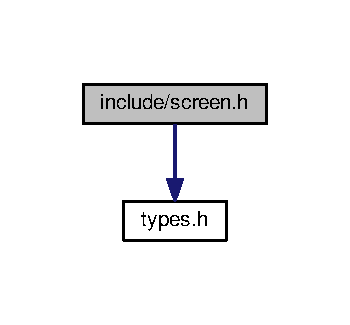
\includegraphics[width=168pt]{screen_8h__incl}
\end{center}
\end{figure}
\subsection*{Macros}
\begin{DoxyCompactItemize}
\item 
\#define \hyperlink{screen_8h_aab63df3ae7b979d59ea0188055ea0763}{S\+C\+R\+E\+E\+N\+\_\+\+M\+A\+X\+\_\+\+S\+TR}~80
\end{DoxyCompactItemize}
\subsection*{Typedefs}
\begin{DoxyCompactItemize}
\item 
typedef struct \+\_\+\+Area \hyperlink{screen_8h_acfdfc42f6522d75fa3c16713afde8127}{Area}\hypertarget{screen_8h_acfdfc42f6522d75fa3c16713afde8127}{}\label{screen_8h_acfdfc42f6522d75fa3c16713afde8127}

\begin{DoxyCompactList}\small\item\em It holds the necessary data to manage areas. \end{DoxyCompactList}\end{DoxyCompactItemize}
\subsection*{Functions}
\begin{Indent}{\bf screen\+\_\+init}\par
{\em It allocates memory for the scree usage

\begin{DoxyAuthor}{Author}
Profesores P\+P\+R\+OG edited by Alejandro Pascual 
\end{DoxyAuthor}
\begin{DoxyVersion}{Version}
1.\+0 
\end{DoxyVersion}
\begin{DoxyDate}{Date}
11-\/01-\/2017 
\end{DoxyDate}

\begin{DoxyParams}{Parameters}
{\em An} & int with the color of the screen. \\
\hline
\end{DoxyParams}
\begin{DoxyReturn}{Returns}
A void, without any relevant information. 
\end{DoxyReturn}
}\begin{DoxyCompactItemize}
\item 
void {\bfseries screen\+\_\+init} (int color)\hypertarget{screen_8h_ad79395b1616e4fadfc671dc806baef85}{}\label{screen_8h_ad79395b1616e4fadfc671dc806baef85}

\end{DoxyCompactItemize}
\end{Indent}
\begin{Indent}{\bf screen\+\_\+destroy}\par
{\em It frees the memory allocated by a screen.

\begin{DoxyAuthor}{Author}
Profesores P\+P\+R\+OG 
\end{DoxyAuthor}
\begin{DoxyVersion}{Version}
1.\+0 
\end{DoxyVersion}
\begin{DoxyDate}{Date}
11-\/01-\/2017 
\end{DoxyDate}
\begin{DoxyReturn}{Returns}
A void, without any relevant information. 
\end{DoxyReturn}
}\begin{DoxyCompactItemize}
\item 
void {\bfseries screen\+\_\+destroy} ()\hypertarget{screen_8h_a3d6d82dde2bb4f3ddc4d276dabe313ef}{}\label{screen_8h_a3d6d82dde2bb4f3ddc4d276dabe313ef}

\end{DoxyCompactItemize}
\end{Indent}
\begin{Indent}{\bf screen\+\_\+paint}\par
{\em It paints the game information on the screen.

\begin{DoxyAuthor}{Author}
Profesores P\+P\+R\+OG 
\end{DoxyAuthor}
\begin{DoxyVersion}{Version}
1.\+0 
\end{DoxyVersion}
\begin{DoxyDate}{Date}
11-\/01-\/2017 
\end{DoxyDate}
\begin{DoxyReturn}{Returns}
A void, without any relevant information. 
\end{DoxyReturn}
}\begin{DoxyCompactItemize}
\item 
void {\bfseries screen\+\_\+paint} ()\hypertarget{screen_8h_a3eaa0547a956d39b6c55c9593524e0d1}{}\label{screen_8h_a3eaa0547a956d39b6c55c9593524e0d1}

\end{DoxyCompactItemize}
\end{Indent}
\begin{Indent}{\bf screen\+\_\+gets}\par
{\em It gets the information to print on the screen from a character string.

\begin{DoxyAuthor}{Author}
Profesores P\+P\+R\+OG 
\end{DoxyAuthor}
\begin{DoxyVersion}{Version}
1.\+0 
\end{DoxyVersion}
\begin{DoxyDate}{Date}
11-\/01-\/2017 
\end{DoxyDate}

\begin{DoxyParams}{Parameters}
{\em char$\ast$} & -\/$>$ a string with the data to print on the screen. \\
\hline
\end{DoxyParams}
\begin{DoxyReturn}{Returns}
A void, without any information. 
\end{DoxyReturn}
}\begin{DoxyCompactItemize}
\item 
void {\bfseries screen\+\_\+gets} (char $\ast$)\hypertarget{screen_8h_a62c596823eb416f448fbef84db4ac6e8}{}\label{screen_8h_a62c596823eb416f448fbef84db4ac6e8}

\end{DoxyCompactItemize}
\end{Indent}
\begin{Indent}{\bf screen\+\_\+area\+\_\+init}\par
{\em It initializes the area we will be printing in of a screen (the white boxes).

\begin{DoxyAuthor}{Author}
Profesores P\+P\+R\+OG 
\end{DoxyAuthor}
\begin{DoxyVersion}{Version}
1.\+0 
\end{DoxyVersion}
\begin{DoxyDate}{Date}
11-\/01-\/2017 
\end{DoxyDate}

\begin{DoxyParams}{Parameters}
{\em int} & -\/$>$ an integer with the X coordinates to start from. \\
\hline
{\em int} & -\/$>$ an integer with the Y coordinates to start from. \\
\hline
{\em int} & -\/$>$ an integer with the width of the area. \\
\hline
{\em int} & -\/$>$ an integer with the height of the area. \\
\hline
{\em int} & -\/$>$ an integer with the foreground color of the area. \\
\hline
{\em int} & -\/$>$ an integer with the background color of the area. \\
\hline
{\em B\+O\+OL} & -\/$>$ A B\+O\+OL that determines if the area has border or not. \\
\hline
\end{DoxyParams}
\begin{DoxyReturn}{Returns}
An Area, with the area created. 
\end{DoxyReturn}
}\begin{DoxyCompactItemize}
\item 
\hyperlink{screen_8h_acfdfc42f6522d75fa3c16713afde8127}{Area} $\ast$ {\bfseries screen\+\_\+area\+\_\+init} (int x, int y, int width, int height, int fg\+\_\+color, int bg\+\_\+color, \hyperlink{types_8h_a3e5b8192e7d9ffaf3542f1210aec18dd}{B\+O\+OL} has\+\_\+border)\hypertarget{screen_8h_a82bb72a86ea8de0bb5650e546607c4df}{}\label{screen_8h_a82bb72a86ea8de0bb5650e546607c4df}

\end{DoxyCompactItemize}
\end{Indent}
\begin{Indent}{\bf screen\+\_\+area\+\_\+destroy}\par
{\em It frees the memory allocated by an area of the screen.

\begin{DoxyAuthor}{Author}
Profesores P\+P\+R\+OG 
\end{DoxyAuthor}
\begin{DoxyVersion}{Version}
1.\+0 
\end{DoxyVersion}
\begin{DoxyDate}{Date}
11-\/01-\/2017 
\end{DoxyDate}

\begin{DoxyParams}{Parameters}
{\em Area$\ast$} & -\/$>$ an area to destroy. \\
\hline
\end{DoxyParams}
\begin{DoxyReturn}{Returns}
A void, without any relevant information. 
\end{DoxyReturn}
}\begin{DoxyCompactItemize}
\item 
void {\bfseries screen\+\_\+area\+\_\+destroy} (\hyperlink{screen_8h_acfdfc42f6522d75fa3c16713afde8127}{Area} $\ast$)\hypertarget{screen_8h_ab53599fd87dafbb35ae8baa0a4abfdc4}{}\label{screen_8h_ab53599fd87dafbb35ae8baa0a4abfdc4}

\end{DoxyCompactItemize}
\end{Indent}
\begin{Indent}{\bf screen\+\_\+area\+\_\+clear}\par
{\em It empties an area of the screen (like cleaning it).

\begin{DoxyAuthor}{Author}
Profesores P\+P\+R\+OG 
\end{DoxyAuthor}
\begin{DoxyVersion}{Version}
1.\+0 
\end{DoxyVersion}
\begin{DoxyDate}{Date}
11-\/01-\/2017 
\end{DoxyDate}

\begin{DoxyParams}{Parameters}
{\em Area$\ast$} & -\/$>$ the area to clear \\
\hline
\end{DoxyParams}
\begin{DoxyReturn}{Returns}
A void, without any relevant information. 
\end{DoxyReturn}
}\begin{DoxyCompactItemize}
\item 
void {\bfseries screen\+\_\+area\+\_\+clear} (\hyperlink{screen_8h_acfdfc42f6522d75fa3c16713afde8127}{Area} $\ast$)\hypertarget{screen_8h_a17da7f04b6fb964b653a750cbb90481a}{}\label{screen_8h_a17da7f04b6fb964b653a750cbb90481a}

\end{DoxyCompactItemize}
\end{Indent}
\begin{Indent}{\bf screen\+\_\+area\+\_\+reset\+\_\+cursor}\par
{\em It resets the cursor.

\begin{DoxyAuthor}{Author}
Profesores P\+P\+R\+OG 
\end{DoxyAuthor}
\begin{DoxyVersion}{Version}
1.\+0 
\end{DoxyVersion}
\begin{DoxyDate}{Date}
11-\/01-\/2017 
\end{DoxyDate}

\begin{DoxyParams}{Parameters}
{\em Area$\ast$} & -\/$>$ the area to reset cursor. \\
\hline
\end{DoxyParams}
\begin{DoxyReturn}{Returns}
A void, without any relevant information. 
\end{DoxyReturn}
}\begin{DoxyCompactItemize}
\item 
void {\bfseries screen\+\_\+area\+\_\+reset\+\_\+cursor} (\hyperlink{screen_8h_acfdfc42f6522d75fa3c16713afde8127}{Area} $\ast$)\hypertarget{screen_8h_a42ae451a0b8eba2b30f228a10d472907}{}\label{screen_8h_a42ae451a0b8eba2b30f228a10d472907}

\end{DoxyCompactItemize}
\end{Indent}
\begin{Indent}{\bf screen\+\_\+area\+\_\+puts}\par
{\em It puts on the area the given info.

\begin{DoxyAuthor}{Author}
Profesores P\+P\+R\+OG 
\end{DoxyAuthor}
\begin{DoxyVersion}{Version}
1.\+0 
\end{DoxyVersion}
\begin{DoxyDate}{Date}
11-\/01-\/2017 
\end{DoxyDate}

\begin{DoxyParams}{Parameters}
{\em Area$\ast$} & -\/$>$ to print in. \\
\hline
{\em char$\ast$} & -\/$>$ a string with the info to print. \\
\hline
\end{DoxyParams}
\begin{DoxyReturn}{Returns}
A void, without any relevant information. 
\end{DoxyReturn}
}\begin{DoxyCompactItemize}
\item 
void {\bfseries screen\+\_\+area\+\_\+puts} (\hyperlink{screen_8h_acfdfc42f6522d75fa3c16713afde8127}{Area} $\ast$, char $\ast$)\hypertarget{screen_8h_aabbb0f5e6225cf095d57b0f3abcc8bb9}{}\label{screen_8h_aabbb0f5e6225cf095d57b0f3abcc8bb9}

\end{DoxyCompactItemize}
\end{Indent}
\begin{Indent}{\bf screen\+\_\+color\+\_\+box}\par
{\em It paints a colored square on the given coordinates.

\begin{DoxyAuthor}{Author}
Alejandro Pascual 
\end{DoxyAuthor}
\begin{DoxyVersion}{Version}
1.\+0 
\end{DoxyVersion}
\begin{DoxyDate}{Date}
04-\/04-\/2017 
\end{DoxyDate}

\begin{DoxyParams}{Parameters}
{\em int} & -\/$>$ an integer with the X coordinates to start from. \\
\hline
{\em int} & -\/$>$ an integer with the Y coordinates to start from. \\
\hline
{\em int} & -\/$>$ an integer with the width of the area. \\
\hline
{\em int} & -\/$>$ an integer with the height of the area. \\
\hline
{\em int} & -\/$>$ an integer with the foreground color of the area. \\
\hline
{\em int} & -\/$>$ an integer with the background color of the area. \\
\hline
\end{DoxyParams}
\begin{DoxyReturn}{Returns}
A void, without any relevant information. 
\end{DoxyReturn}
}\begin{DoxyCompactItemize}
\item 
void {\bfseries screen\+\_\+color\+\_\+box} (int x, int y, int width, int height, int fg\+\_\+color, int bg\+\_\+color)\hypertarget{screen_8h_a8cc1a241a2c2b129ac53c3ef5a7c02f8}{}\label{screen_8h_a8cc1a241a2c2b129ac53c3ef5a7c02f8}

\end{DoxyCompactItemize}
\end{Indent}
\begin{Indent}{\bf screen\+\_\+add\+\_\+border}\par
{\em It puts a border on the given area.

\begin{DoxyAuthor}{Author}
Alejandro Pascual 
\end{DoxyAuthor}
\begin{DoxyVersion}{Version}
1.\+0 
\end{DoxyVersion}
\begin{DoxyDate}{Date}
04-\/04-\/2018 
\end{DoxyDate}

\begin{DoxyParams}{Parameters}
{\em int} & -\/$>$ an integer with the X coordinates to start from. \\
\hline
{\em int} & -\/$>$ an integer with the Y coordinates to start from. \\
\hline
{\em int} & -\/$>$ an integer with the width of the area. \\
\hline
{\em int} & -\/$>$ an integer with the height of the area. \\
\hline
{\em int} & -\/$>$ an integer with the foreground color of the area. \\
\hline
{\em int} & -\/$>$ an integer with the background color of the area. \\
\hline
\end{DoxyParams}
\begin{DoxyReturn}{Returns}
A void, without any relevant information. 
\end{DoxyReturn}
}\begin{DoxyCompactItemize}
\item 
void {\bfseries screen\+\_\+add\+\_\+border} (int x, int y, int width, int height, int fg\+\_\+color, int bg\+\_\+color)\hypertarget{screen_8h_af8060f8d91b3fd4c1423727f4c99727c}{}\label{screen_8h_af8060f8d91b3fd4c1423727f4c99727c}

\end{DoxyCompactItemize}
\end{Indent}


\subsection{Detailed Description}
It defines the screen functions. 

\begin{DoxyAuthor}{Author}
Profesores P\+P\+R\+OG edited by Alejandro Pascual 
\end{DoxyAuthor}
\begin{DoxyVersion}{Version}
1.\+0 
\end{DoxyVersion}
\begin{DoxyDate}{Date}
11-\/01-\/2017 
\end{DoxyDate}
\begin{DoxyCopyright}{Copyright}
G\+NU Public License 
\end{DoxyCopyright}


\subsection{Macro Definition Documentation}
\index{screen.\+h@{screen.\+h}!S\+C\+R\+E\+E\+N\+\_\+\+M\+A\+X\+\_\+\+S\+TR@{S\+C\+R\+E\+E\+N\+\_\+\+M\+A\+X\+\_\+\+S\+TR}}
\index{S\+C\+R\+E\+E\+N\+\_\+\+M\+A\+X\+\_\+\+S\+TR@{S\+C\+R\+E\+E\+N\+\_\+\+M\+A\+X\+\_\+\+S\+TR}!screen.\+h@{screen.\+h}}
\subsubsection[{\texorpdfstring{S\+C\+R\+E\+E\+N\+\_\+\+M\+A\+X\+\_\+\+S\+TR}{SCREEN_MAX_STR}}]{\setlength{\rightskip}{0pt plus 5cm}\#define S\+C\+R\+E\+E\+N\+\_\+\+M\+A\+X\+\_\+\+S\+TR~80}\hypertarget{screen_8h_aab63df3ae7b979d59ea0188055ea0763}{}\label{screen_8h_aab63df3ae7b979d59ea0188055ea0763}
The maximum size of an string to print 
\hypertarget{set_8h}{}\section{include/set.h File Reference}
\label{set_8h}\index{include/set.\+h@{include/set.\+h}}


It defines the A\+DT Set, which manages a list of Ids.  


{\ttfamily \#include \char`\"{}types.\+h\char`\"{}}\\*
Include dependency graph for set.\+h\+:\nopagebreak
\begin{figure}[H]
\begin{center}
\leavevmode
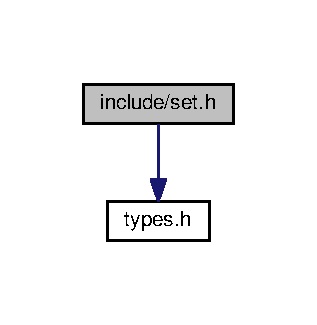
\includegraphics[width=152pt]{set_8h__incl}
\end{center}
\end{figure}
\subsection*{Typedefs}
\begin{DoxyCompactItemize}
\item 
typedef struct \+\_\+\+Set \hyperlink{set_8h_a6d3b7f7c92cbb4577ef3ef7ddbf93161}{Set}\hypertarget{set_8h_a6d3b7f7c92cbb4577ef3ef7ddbf93161}{}\label{set_8h_a6d3b7f7c92cbb4577ef3ef7ddbf93161}

\begin{DoxyCompactList}\small\item\em It holds the necessary data to manage a set. \end{DoxyCompactList}\end{DoxyCompactItemize}
\subsection*{Functions}
\begin{Indent}{\bf set\+\_\+create}\par
{\em It allocates the memory for a Set structure.

\begin{DoxyAuthor}{Author}
Alejandro Pascual 
\end{DoxyAuthor}
\begin{DoxyVersion}{Version}
1.\+0 
\end{DoxyVersion}
\begin{DoxyDate}{Date}
26-\/02-\/2018 
\end{DoxyDate}
\begin{DoxyReturn}{Returns}
A Set$\ast$, with the memory allocated and all the fields initialized. 
\end{DoxyReturn}
}\begin{DoxyCompactItemize}
\item 
\hyperlink{set_8h_a6d3b7f7c92cbb4577ef3ef7ddbf93161}{Set} $\ast$ {\bfseries set\+\_\+create} ()\hypertarget{set_8h_abcc73b7ad3913fc92dd95d366c9c8687}{}\label{set_8h_abcc73b7ad3913fc92dd95d366c9c8687}

\end{DoxyCompactItemize}
\end{Indent}
\begin{Indent}{\bf set\+\_\+destroy}\par
{\em It frees the memory for a Set structure.

\begin{DoxyAuthor}{Author}
Alejandro Pascual 
\end{DoxyAuthor}
\begin{DoxyVersion}{Version}
1.\+0 
\end{DoxyVersion}
\begin{DoxyDate}{Date}
26-\/02-\/2018 
\end{DoxyDate}

\begin{DoxyParams}{Parameters}
{\em Set$\ast$} & -\/$>$ a set whose memory will be deallocated. \\
\hline
\end{DoxyParams}
\begin{DoxyReturn}{Returns}
A S\+T\+A\+T\+US, which indicates if the process was executed successfully or not. 
\end{DoxyReturn}
}\begin{DoxyCompactItemize}
\item 
\hyperlink{types_8h_a32c27cc471df37f4fc818d65de0a56c4}{S\+T\+A\+T\+US} {\bfseries set\+\_\+destroy} (\hyperlink{set_8h_a6d3b7f7c92cbb4577ef3ef7ddbf93161}{Set} $\ast$)\hypertarget{set_8h_abb90ac68e70fea10a44ee00e42d47d85}{}\label{set_8h_abb90ac68e70fea10a44ee00e42d47d85}

\end{DoxyCompactItemize}
\end{Indent}
\begin{Indent}{\bf set\+\_\+add}\par
{\em It adds an Id to the Set

\begin{DoxyAuthor}{Author}
Alejandro Pascual 
\end{DoxyAuthor}
\begin{DoxyVersion}{Version}
1.\+0 
\end{DoxyVersion}
\begin{DoxyDate}{Date}
26-\/02-\/2018 
\end{DoxyDate}

\begin{DoxyParams}{Parameters}
{\em Set$\ast$} & -\/$>$ a set in which the id will be added. \\
\hline
{\em Id} & -\/$>$ the id which will be added to the set. \\
\hline
\end{DoxyParams}
\begin{DoxyReturn}{Returns}
A S\+T\+A\+T\+US, which indicates if the process was executed successfully or not. 
\end{DoxyReturn}
}\begin{DoxyCompactItemize}
\item 
\hyperlink{types_8h_a32c27cc471df37f4fc818d65de0a56c4}{S\+T\+A\+T\+US} {\bfseries set\+\_\+add} (\hyperlink{set_8h_a6d3b7f7c92cbb4577ef3ef7ddbf93161}{Set} $\ast$, \hyperlink{types_8h_a845e604fb28f7e3d97549da3448149d3}{Id})\hypertarget{set_8h_ada6e5ed947e3b64276501c5337676fba}{}\label{set_8h_ada6e5ed947e3b64276501c5337676fba}

\end{DoxyCompactItemize}
\end{Indent}
\begin{Indent}{\bf set\+\_\+del}\par
{\em It removes an Id of the Set

\begin{DoxyAuthor}{Author}
Alejandro Pascual 
\end{DoxyAuthor}
\begin{DoxyVersion}{Version}
1.\+0 
\end{DoxyVersion}
\begin{DoxyDate}{Date}
26-\/02-\/2018 
\end{DoxyDate}

\begin{DoxyParams}{Parameters}
{\em Set$\ast$} & -\/$>$ the set from which the id will be removed. \\
\hline
{\em Id} & -\/$>$ the id to be removed from the set. \\
\hline
\end{DoxyParams}
\begin{DoxyReturn}{Returns}
A S\+T\+A\+T\+US, which indicates if the process was executed successfully or not. 
\end{DoxyReturn}
}\begin{DoxyCompactItemize}
\item 
\hyperlink{types_8h_a32c27cc471df37f4fc818d65de0a56c4}{S\+T\+A\+T\+US} {\bfseries set\+\_\+del} (\hyperlink{set_8h_a6d3b7f7c92cbb4577ef3ef7ddbf93161}{Set} $\ast$, \hyperlink{types_8h_a845e604fb28f7e3d97549da3448149d3}{Id})\hypertarget{set_8h_a0f85803b8c26d13d756ef04bbc0e5b75}{}\label{set_8h_a0f85803b8c26d13d756ef04bbc0e5b75}

\end{DoxyCompactItemize}
\end{Indent}
\begin{Indent}{\bf set\+\_\+get\+\_\+id}\par
{\em It returns the id of the indicated position of the Set.

\begin{DoxyAuthor}{Author}
Alejandro Pascual 
\end{DoxyAuthor}
\begin{DoxyVersion}{Version}
1.\+0 
\end{DoxyVersion}
\begin{DoxyDate}{Date}
26-\/02-\/2018 
\end{DoxyDate}

\begin{DoxyParams}{Parameters}
{\em Set$\ast$} & -\/$>$ the set we will get the id from. \\
\hline
{\em int} & -\/$>$ an integer which indicates the position of the Id in the Set. \\
\hline
\end{DoxyParams}
\begin{DoxyReturn}{Returns}
The Id of the selected position of the Set. 
\end{DoxyReturn}
}\begin{DoxyCompactItemize}
\item 
\hyperlink{types_8h_a845e604fb28f7e3d97549da3448149d3}{Id} {\bfseries set\+\_\+get\+\_\+id} (\hyperlink{set_8h_a6d3b7f7c92cbb4577ef3ef7ddbf93161}{Set} $\ast$, int id\+\_\+position)\hypertarget{set_8h_a5abb6ac8c6502c1da946bfdaeca19671}{}\label{set_8h_a5abb6ac8c6502c1da946bfdaeca19671}

\end{DoxyCompactItemize}
\end{Indent}
\begin{Indent}{\bf set\+\_\+get\+\_\+id\+\_\+position}\par
{\em It returns the position of the specified Id in the Set.

\begin{DoxyAuthor}{Author}
Alejandro Pascual 
\end{DoxyAuthor}
\begin{DoxyVersion}{Version}
1.\+0 
\end{DoxyVersion}
\begin{DoxyDate}{Date}
26-\/02-\/2018 
\end{DoxyDate}

\begin{DoxyParams}{Parameters}
{\em Set$\ast$} & -\/$>$ the set we are going to search in. \\
\hline
{\em Id} & -\/$>$ the id whose position in the Set will be returned. \\
\hline
\end{DoxyParams}
\begin{DoxyReturn}{Returns}
The position of the specified Id in the Set. 
\end{DoxyReturn}
}\begin{DoxyCompactItemize}
\item 
int {\bfseries set\+\_\+get\+\_\+id\+\_\+position} (\hyperlink{set_8h_a6d3b7f7c92cbb4577ef3ef7ddbf93161}{Set} $\ast$, \hyperlink{types_8h_a845e604fb28f7e3d97549da3448149d3}{Id})\hypertarget{set_8h_a3660481717cfdf4a4dfe8b1f19b7a533}{}\label{set_8h_a3660481717cfdf4a4dfe8b1f19b7a533}

\end{DoxyCompactItemize}
\end{Indent}
\begin{Indent}{\bf set\+\_\+get\+\_\+ids\+\_\+number}\par
{\em It returns the number of Ids stored in the Set.

\begin{DoxyAuthor}{Author}
Alejandro Pascual 
\end{DoxyAuthor}
\begin{DoxyVersion}{Version}
1.\+0 
\end{DoxyVersion}
\begin{DoxyDate}{Date}
26-\/02-\/2018 
\end{DoxyDate}

\begin{DoxyParams}{Parameters}
{\em Set$\ast$} & -\/$>$ the set we will get the number of ids from. \\
\hline
\end{DoxyParams}
\begin{DoxyReturn}{Returns}
The number of Ids stored in the Set. 
\end{DoxyReturn}
}\begin{DoxyCompactItemize}
\item 
int {\bfseries set\+\_\+get\+\_\+ids\+\_\+number} (\hyperlink{set_8h_a6d3b7f7c92cbb4577ef3ef7ddbf93161}{Set} $\ast$)\hypertarget{set_8h_accbe3acf1d0d4ee55029f1e407aa3047}{}\label{set_8h_accbe3acf1d0d4ee55029f1e407aa3047}

\end{DoxyCompactItemize}
\end{Indent}
\begin{Indent}{\bf set\+\_\+is\+\_\+empty}\par
{\em It returns a B\+O\+OL, which indicates if the Set is empty.

\begin{DoxyAuthor}{Author}
Alejandro Pascual 
\end{DoxyAuthor}
\begin{DoxyVersion}{Version}
1.\+0 
\end{DoxyVersion}
\begin{DoxyDate}{Date}
26-\/02-\/2018 
\end{DoxyDate}

\begin{DoxyParams}{Parameters}
{\em Set$\ast$} & -\/$>$ the set we are going to check if empty or not. \\
\hline
\end{DoxyParams}
\begin{DoxyReturn}{Returns}
A B\+O\+OL, which indicates if the Set is empty. 
\end{DoxyReturn}
}\begin{DoxyCompactItemize}
\item 
\hyperlink{types_8h_a3e5b8192e7d9ffaf3542f1210aec18dd}{B\+O\+OL} {\bfseries set\+\_\+is\+\_\+empty} (\hyperlink{set_8h_a6d3b7f7c92cbb4577ef3ef7ddbf93161}{Set} $\ast$)\hypertarget{set_8h_a090b890a13d4bade465b46ffac4dd09a}{}\label{set_8h_a090b890a13d4bade465b46ffac4dd09a}

\end{DoxyCompactItemize}
\end{Indent}
\begin{Indent}{\bf set\+\_\+is\+\_\+full}\par
{\em It returns a B\+O\+OL, which indicates if the Set is full.

\begin{DoxyAuthor}{Author}
Alejandro Pascual 
\end{DoxyAuthor}
\begin{DoxyVersion}{Version}
1.\+0 
\end{DoxyVersion}
\begin{DoxyDate}{Date}
26-\/02-\/2018 
\end{DoxyDate}

\begin{DoxyParams}{Parameters}
{\em Set$\ast$} & -\/$>$ the set we are going to check if full. \\
\hline
\end{DoxyParams}
\begin{DoxyReturn}{Returns}
A B\+O\+OL, which indicates if the Set is full. 
\end{DoxyReturn}
}\begin{DoxyCompactItemize}
\item 
\hyperlink{types_8h_a3e5b8192e7d9ffaf3542f1210aec18dd}{B\+O\+OL} {\bfseries set\+\_\+is\+\_\+full} (\hyperlink{set_8h_a6d3b7f7c92cbb4577ef3ef7ddbf93161}{Set} $\ast$)\hypertarget{set_8h_ae0aab790dc0dac183d5e809d7e5a72f1}{}\label{set_8h_ae0aab790dc0dac183d5e809d7e5a72f1}

\end{DoxyCompactItemize}
\end{Indent}
\begin{Indent}{\bf set\+\_\+print}\par
{\em It prints the info of the passed Set.

\begin{DoxyAuthor}{Author}
Alejandro Pascual 
\end{DoxyAuthor}
\begin{DoxyVersion}{Version}
1.\+0 
\end{DoxyVersion}
\begin{DoxyDate}{Date}
26-\/02-\/2018 
\end{DoxyDate}

\begin{DoxyParams}{Parameters}
{\em Set$\ast$} & -\/$>$ the set to be used. \\
\hline
\end{DoxyParams}
\begin{DoxyReturn}{Returns}
A S\+T\+A\+T\+US, which indicates if the process was executed successfully or not.
\end{DoxyReturn}
N\+O\+TE\+: This function was created for debugging purposes only and it is not used in the normal execution of the game. }\begin{DoxyCompactItemize}
\item 
\hyperlink{types_8h_a32c27cc471df37f4fc818d65de0a56c4}{S\+T\+A\+T\+US} {\bfseries set\+\_\+print} (\hyperlink{set_8h_a6d3b7f7c92cbb4577ef3ef7ddbf93161}{Set} $\ast$)\hypertarget{set_8h_a3e17364bd35023c2aca6576766a02574}{}\label{set_8h_a3e17364bd35023c2aca6576766a02574}

\end{DoxyCompactItemize}
\end{Indent}


\subsection{Detailed Description}
It defines the A\+DT Set, which manages a list of Ids. 

\begin{DoxyAuthor}{Author}
Victor Yrazusta and Alejandro Pascual 
\end{DoxyAuthor}
\begin{DoxyDate}{Date}
23-\/02-\/2017 
\end{DoxyDate}
\begin{DoxyCopyright}{Copyright}
G\+NU Public License 
\end{DoxyCopyright}

\hypertarget{space_8h}{}\section{include/space.h File Reference}
\label{space_8h}\index{include/space.\+h@{include/space.\+h}}


It defines the space and the needed functions.  


{\ttfamily \#include \char`\"{}types.\+h\char`\"{}}\\*
Include dependency graph for space.\+h\+:\nopagebreak
\begin{figure}[H]
\begin{center}
\leavevmode
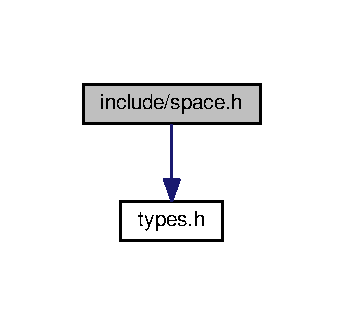
\includegraphics[width=165pt]{space_8h__incl}
\end{center}
\end{figure}
This graph shows which files directly or indirectly include this file\+:\nopagebreak
\begin{figure}[H]
\begin{center}
\leavevmode
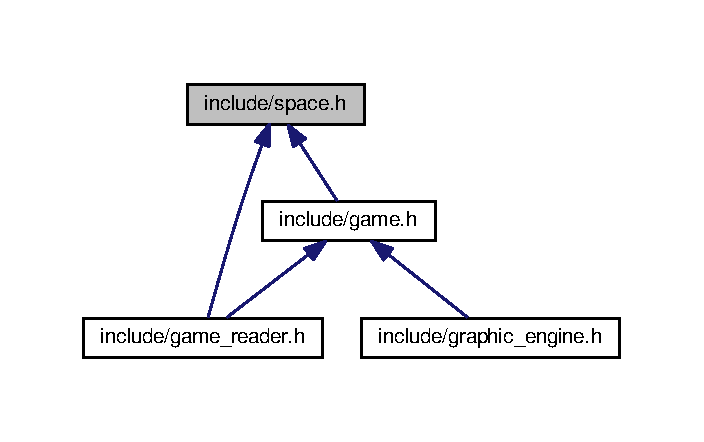
\includegraphics[width=338pt]{space_8h__dep__incl}
\end{center}
\end{figure}
\subsection*{Typedefs}
\begin{DoxyCompactItemize}
\item 
typedef struct \+\_\+\+Space \hyperlink{space_8h_a67533ffc2b70463baecc38fb0629bbfc}{Space}\hypertarget{space_8h_a67533ffc2b70463baecc38fb0629bbfc}{}\label{space_8h_a67533ffc2b70463baecc38fb0629bbfc}

\begin{DoxyCompactList}\small\item\em It holds the necessary data to manage a space. \end{DoxyCompactList}\end{DoxyCompactItemize}
\subsection*{Functions}
\begin{Indent}{\bf space\+\_\+create}\par
{\em It creates a space with the id passed.

\begin{DoxyAuthor}{Author}
Profesores P\+P\+R\+OG edited by Eric Morales 
\end{DoxyAuthor}
\begin{DoxyVersion}{Version}
2.\+0 
\end{DoxyVersion}
\begin{DoxyDate}{Date}
18-\/03-\/2018 
\end{DoxyDate}

\begin{DoxyParams}{Parameters}
{\em Id} & with the id for the new space. \\
\hline
\end{DoxyParams}
\begin{DoxyReturn}{Returns}
A Link$\ast$, which points towards the created space. 
\end{DoxyReturn}
}\begin{DoxyCompactItemize}
\item 
\hyperlink{space_8h_a67533ffc2b70463baecc38fb0629bbfc}{Space} $\ast$ {\bfseries space\+\_\+create} (\hyperlink{types_8h_a845e604fb28f7e3d97549da3448149d3}{Id})\hypertarget{space_8h_a6b9b52e123aa674b45940c4d6d4163f7}{}\label{space_8h_a6b9b52e123aa674b45940c4d6d4163f7}

\end{DoxyCompactItemize}
\end{Indent}
\begin{Indent}{\bf space\+\_\+destroy}\par
{\em It destroys the space passed.

\begin{DoxyAuthor}{Author}
Profesores P\+P\+R\+OG edited by Eric Morales 
\end{DoxyAuthor}
\begin{DoxyVersion}{Version}
2.\+0 
\end{DoxyVersion}
\begin{DoxyDate}{Date}
13-\/01-\/2015 
\end{DoxyDate}

\begin{DoxyParams}{Parameters}
{\em Space$\ast$} & with the space which will be destroyed. \\
\hline
\end{DoxyParams}
\begin{DoxyReturn}{Returns}
A S\+T\+A\+T\+US which indicates whether the operation could be executed correctly. 
\end{DoxyReturn}
}\begin{DoxyCompactItemize}
\item 
\hyperlink{types_8h_a32c27cc471df37f4fc818d65de0a56c4}{S\+T\+A\+T\+US} {\bfseries space\+\_\+destroy} (\hyperlink{space_8h_a67533ffc2b70463baecc38fb0629bbfc}{Space} $\ast$)\hypertarget{space_8h_aea767528288845a8bc3d0b4c5871d603}{}\label{space_8h_aea767528288845a8bc3d0b4c5871d603}

\end{DoxyCompactItemize}
\end{Indent}
\begin{Indent}{\bf space\+\_\+set\+\_\+name}\par
{\em It changes the name of the passed space.

\begin{DoxyAuthor}{Author}
Profesores P\+P\+R\+OG 
\end{DoxyAuthor}
\begin{DoxyVersion}{Version}
1.\+0 
\end{DoxyVersion}
\begin{DoxyDate}{Date}
13-\/01-\/2015 
\end{DoxyDate}

\begin{DoxyParams}{Parameters}
{\em Space$\ast$} & with the space whose name will be changed. \\
\hline
{\em schar} & with the new name for the space. \\
\hline
\end{DoxyParams}
\begin{DoxyReturn}{Returns}
A S\+T\+A\+T\+US which indicates whether the operation could be executed correctly. 
\end{DoxyReturn}
}\begin{DoxyCompactItemize}
\item 
\hyperlink{types_8h_a32c27cc471df37f4fc818d65de0a56c4}{S\+T\+A\+T\+US} {\bfseries space\+\_\+set\+\_\+name} (\hyperlink{space_8h_a67533ffc2b70463baecc38fb0629bbfc}{Space} $\ast$, char $\ast$name)\hypertarget{space_8h_ab1fc1ed4a1846be6efbcd855c72ea440}{}\label{space_8h_ab1fc1ed4a1846be6efbcd855c72ea440}

\end{DoxyCompactItemize}
\end{Indent}
\begin{Indent}{\bf space\+\_\+set\+\_\+north}\par
{\em It changes the north of the passed space.

\begin{DoxyAuthor}{Author}
Profesores P\+P\+R\+OG 
\end{DoxyAuthor}
\begin{DoxyVersion}{Version}
2.\+0 
\end{DoxyVersion}
\begin{DoxyDate}{Date}
18-\/03-\/2018 
\end{DoxyDate}

\begin{DoxyParams}{Parameters}
{\em Space$\ast$} & with the space whose north will be changed. \\
\hline
{\em Id} & with the new north link for the space. \\
\hline
\end{DoxyParams}
\begin{DoxyReturn}{Returns}
A S\+T\+A\+T\+US which indicates whether the operation could be executed correctly. 
\end{DoxyReturn}
}\begin{DoxyCompactItemize}
\item 
\hyperlink{types_8h_a32c27cc471df37f4fc818d65de0a56c4}{S\+T\+A\+T\+US} {\bfseries space\+\_\+set\+\_\+north} (\hyperlink{space_8h_a67533ffc2b70463baecc38fb0629bbfc}{Space} $\ast$, \hyperlink{types_8h_a845e604fb28f7e3d97549da3448149d3}{Id})\hypertarget{space_8h_a879742b71ae8398cf2e6f566f61ffddf}{}\label{space_8h_a879742b71ae8398cf2e6f566f61ffddf}

\end{DoxyCompactItemize}
\end{Indent}
\begin{Indent}{\bf space\+\_\+set\+\_\+west}\par
{\em It changes the west of the passed space.

\begin{DoxyAuthor}{Author}
Profesores P\+P\+R\+OG 
\end{DoxyAuthor}
\begin{DoxyVersion}{Version}
2.\+0 
\end{DoxyVersion}
\begin{DoxyDate}{Date}
18-\/03-\/2018 
\end{DoxyDate}

\begin{DoxyParams}{Parameters}
{\em Space$\ast$} & with the space whose west will be changed. \\
\hline
{\em Id} & with the new west link for the space. \\
\hline
\end{DoxyParams}
\begin{DoxyReturn}{Returns}
A S\+T\+A\+T\+US which indicates whether the operation could be executed correctly. 
\end{DoxyReturn}
}\begin{DoxyCompactItemize}
\item 
\hyperlink{types_8h_a32c27cc471df37f4fc818d65de0a56c4}{S\+T\+A\+T\+US} {\bfseries space\+\_\+set\+\_\+west} (\hyperlink{space_8h_a67533ffc2b70463baecc38fb0629bbfc}{Space} $\ast$, \hyperlink{types_8h_a845e604fb28f7e3d97549da3448149d3}{Id})\hypertarget{space_8h_a8e3bde8a733af1c19bb4beb7888ac602}{}\label{space_8h_a8e3bde8a733af1c19bb4beb7888ac602}

\end{DoxyCompactItemize}
\end{Indent}
\begin{Indent}{\bf space\+\_\+set\+\_\+south}\par
{\em It changes the south of the passed space.

\begin{DoxyAuthor}{Author}
Profesores P\+P\+R\+OG 
\end{DoxyAuthor}
\begin{DoxyVersion}{Version}
2.\+0 
\end{DoxyVersion}
\begin{DoxyDate}{Date}
18-\/03-\/2018 
\end{DoxyDate}

\begin{DoxyParams}{Parameters}
{\em Space$\ast$} & with the space whose south will be changed. \\
\hline
{\em Id} & with the new south link for the space. \\
\hline
\end{DoxyParams}
\begin{DoxyReturn}{Returns}
A S\+T\+A\+T\+US which indicates whether the operation could be executed correctly. 
\end{DoxyReturn}
}\begin{DoxyCompactItemize}
\item 
\hyperlink{types_8h_a32c27cc471df37f4fc818d65de0a56c4}{S\+T\+A\+T\+US} {\bfseries space\+\_\+set\+\_\+south} (\hyperlink{space_8h_a67533ffc2b70463baecc38fb0629bbfc}{Space} $\ast$, \hyperlink{types_8h_a845e604fb28f7e3d97549da3448149d3}{Id})\hypertarget{space_8h_afa7725a94d5a1c12ded8fd06c7184556}{}\label{space_8h_afa7725a94d5a1c12ded8fd06c7184556}

\end{DoxyCompactItemize}
\end{Indent}
\begin{Indent}{\bf space\+\_\+set\+\_\+east}\par
{\em It changes the east of the passed space.

\begin{DoxyAuthor}{Author}
Profesores P\+P\+R\+OG 
\end{DoxyAuthor}
\begin{DoxyVersion}{Version}
2.\+0 
\end{DoxyVersion}
\begin{DoxyDate}{Date}
18-\/03-\/2018 
\end{DoxyDate}

\begin{DoxyParams}{Parameters}
{\em Space$\ast$} & with the space whose east will be changed. \\
\hline
{\em Id} & with the new east link for the space. \\
\hline
\end{DoxyParams}
\begin{DoxyReturn}{Returns}
A S\+T\+A\+T\+US which indicates whether the operation could be executed correctly. 
\end{DoxyReturn}
}\begin{DoxyCompactItemize}
\item 
\hyperlink{types_8h_a32c27cc471df37f4fc818d65de0a56c4}{S\+T\+A\+T\+US} {\bfseries space\+\_\+set\+\_\+east} (\hyperlink{space_8h_a67533ffc2b70463baecc38fb0629bbfc}{Space} $\ast$, \hyperlink{types_8h_a845e604fb28f7e3d97549da3448149d3}{Id})\hypertarget{space_8h_a2aac336540462ea6e6198e761afba0f0}{}\label{space_8h_a2aac336540462ea6e6198e761afba0f0}

\end{DoxyCompactItemize}
\end{Indent}
\begin{Indent}{\bf space\+\_\+add\+\_\+object}\par
{\em It adds an object to the passed space.

\begin{DoxyAuthor}{Author}
Alejandro Pascual 
\end{DoxyAuthor}
\begin{DoxyVersion}{Version}
1.\+0 
\end{DoxyVersion}
\begin{DoxyDate}{Date}
05-\/03-\/2018 
\end{DoxyDate}

\begin{DoxyParams}{Parameters}
{\em Space$\ast$} & with the space in which the object will be inserted. \\
\hline
{\em Id,with} & the Id of the object to be inserted. \\
\hline
\end{DoxyParams}
\begin{DoxyReturn}{Returns}
A S\+T\+A\+T\+US which indicates whether the operation could be executed correctly. 
\end{DoxyReturn}
}\begin{DoxyCompactItemize}
\item 
\hyperlink{types_8h_a32c27cc471df37f4fc818d65de0a56c4}{S\+T\+A\+T\+US} {\bfseries space\+\_\+add\+\_\+object} (\hyperlink{space_8h_a67533ffc2b70463baecc38fb0629bbfc}{Space} $\ast$, \hyperlink{types_8h_a845e604fb28f7e3d97549da3448149d3}{Id} object\+\_\+id)\hypertarget{space_8h_afd5ac0e44abeebf63ba7434d9e1ab28d}{}\label{space_8h_afd5ac0e44abeebf63ba7434d9e1ab28d}

\end{DoxyCompactItemize}
\end{Indent}
\begin{Indent}{\bf space\+\_\+del\+\_\+object}\par
{\em It deletes an object from the passed space.

\begin{DoxyAuthor}{Author}
Alejandro Pascual 
\end{DoxyAuthor}
\begin{DoxyVersion}{Version}
1.\+0 
\end{DoxyVersion}
\begin{DoxyDate}{Date}
05-\/03-\/2018 
\end{DoxyDate}

\begin{DoxyParams}{Parameters}
{\em Space$\ast$} & with the space in which the object will be deleted. \\
\hline
{\em Id} & with the Id of the object to be deleted. \\
\hline
\end{DoxyParams}
\begin{DoxyReturn}{Returns}
A S\+T\+A\+T\+US which indicates whether the operation could be executed correctly. 
\end{DoxyReturn}
}\begin{DoxyCompactItemize}
\item 
\hyperlink{types_8h_a32c27cc471df37f4fc818d65de0a56c4}{S\+T\+A\+T\+US} {\bfseries space\+\_\+del\+\_\+object} (\hyperlink{space_8h_a67533ffc2b70463baecc38fb0629bbfc}{Space} $\ast$, \hyperlink{types_8h_a845e604fb28f7e3d97549da3448149d3}{Id} object\+\_\+id)\hypertarget{space_8h_a50e1f5b2b31575436fb477679fc3c8c3}{}\label{space_8h_a50e1f5b2b31575436fb477679fc3c8c3}

\end{DoxyCompactItemize}
\end{Indent}
\begin{Indent}{\bf space\+\_\+set\+\_\+graphic\+\_\+description}\par
{\em It changes the graphic description of the passed space.

\begin{DoxyAuthor}{Author}
Alejandro Pascual edited by Eric Morales 
\end{DoxyAuthor}
\begin{DoxyVersion}{Version}
2.\+0 
\end{DoxyVersion}
\begin{DoxyDate}{Date}
05-\/03-\/2018 
\end{DoxyDate}

\begin{DoxyParams}{Parameters}
{\em Space$\ast$} & with the space whose graphic description will be changed. \\
\hline
{\em char} & with the new graphich description for the space. \\
\hline
\end{DoxyParams}
\begin{DoxyReturn}{Returns}
A S\+T\+A\+T\+US which indicates whether the operation could be executed correctly. 
\end{DoxyReturn}
}\begin{DoxyCompactItemize}
\item 
\hyperlink{types_8h_a32c27cc471df37f4fc818d65de0a56c4}{S\+T\+A\+T\+US} {\bfseries space\+\_\+set\+\_\+graphic\+\_\+description} (\hyperlink{space_8h_a67533ffc2b70463baecc38fb0629bbfc}{Space} $\ast$, char graphic\+\_\+description\mbox{[}3\mbox{]}\mbox{[}8\mbox{]})\hypertarget{space_8h_a6564b549993cbc08e8423999d91d5421}{}\label{space_8h_a6564b549993cbc08e8423999d91d5421}

\end{DoxyCompactItemize}
\end{Indent}
\begin{Indent}{\bf object\+\_\+set\+\_\+check}\par
{\em It changes the check description of the passed object to the passed char$\ast$$\ast$.

\begin{DoxyAuthor}{Author}
Eric Morales 
\end{DoxyAuthor}
\begin{DoxyVersion}{Version}
1.\+0 
\end{DoxyVersion}
\begin{DoxyDate}{Date}
26-\/03-\/2018 
\end{DoxyDate}

\begin{DoxyParams}{Parameters}
{\em Object$\ast$,which} & must point towards the object that wants to be renamed. \\
\hline
{\em check,with} & the new description for the object. \\
\hline
\end{DoxyParams}
\begin{DoxyReturn}{Returns}
An S\+T\+A\+T\+US, which could be \char`\"{}\+E\+R\+R\+O\+R\char`\"{} if one of the passed pointers is N\+U\+LL or if the rename fails, or \char`\"{}\+O\+K\char`\"{} otherwise. 
\end{DoxyReturn}
}\begin{DoxyCompactItemize}
\item 
\hyperlink{types_8h_a32c27cc471df37f4fc818d65de0a56c4}{S\+T\+A\+T\+US} {\bfseries space\+\_\+set\+\_\+check} (\hyperlink{space_8h_a67533ffc2b70463baecc38fb0629bbfc}{Space} $\ast$, char check\mbox{[}\hyperlink{types_8h_ae41569a4c2560714ec2b9feb28919682}{M\+A\+X\+\_\+\+C\+H\+E\+C\+K\+\_\+R}\mbox{]}\mbox{[}\hyperlink{types_8h_a9990950cd307079021e49d95eae07c60}{M\+A\+X\+\_\+\+C\+H\+E\+C\+K\+\_\+C}\mbox{]})\hypertarget{space_8h_a2c7b7951bf6f30962f13931b4cabf403}{}\label{space_8h_a2c7b7951bf6f30962f13931b4cabf403}

\end{DoxyCompactItemize}
\end{Indent}
\begin{Indent}{\bf space\+\_\+get\+\_\+id}\par
{\em It returns the Id of the passed space.

\begin{DoxyAuthor}{Author}
Profesores P\+P\+R\+OG 
\end{DoxyAuthor}
\begin{DoxyVersion}{Version}
1.\+0 
\end{DoxyVersion}
\begin{DoxyDate}{Date}
13-\/01-\/2015 
\end{DoxyDate}

\begin{DoxyParams}{Parameters}
{\em Space$\ast$} & with the space whose Id will be returned. \\
\hline
\end{DoxyParams}
\begin{DoxyReturn}{Returns}
An Id with the Id of the space passed. 
\end{DoxyReturn}
}\begin{DoxyCompactItemize}
\item 
\hyperlink{types_8h_a845e604fb28f7e3d97549da3448149d3}{Id} {\bfseries space\+\_\+get\+\_\+id} (\hyperlink{space_8h_a67533ffc2b70463baecc38fb0629bbfc}{Space} $\ast$)\hypertarget{space_8h_aac469ce734efe07d205014dd36d363c2}{}\label{space_8h_aac469ce734efe07d205014dd36d363c2}

\end{DoxyCompactItemize}
\end{Indent}
\begin{Indent}{\bf space\+\_\+get\+\_\+name}\par
{\em It returns the name of the passed space.

\begin{DoxyAuthor}{Author}
Profesores P\+P\+R\+OG 
\end{DoxyAuthor}
\begin{DoxyVersion}{Version}
1.\+0 
\end{DoxyVersion}
\begin{DoxyDate}{Date}
13-\/01-\/2015 
\end{DoxyDate}

\begin{DoxyParams}{Parameters}
{\em Space$\ast$} & with the space whose name will be returned. \\
\hline
\end{DoxyParams}
\begin{DoxyReturn}{Returns}
The name of the space passed. 
\end{DoxyReturn}
}\begin{DoxyCompactItemize}
\item 
const char $\ast$ {\bfseries space\+\_\+get\+\_\+name} (\hyperlink{space_8h_a67533ffc2b70463baecc38fb0629bbfc}{Space} $\ast$)\hypertarget{space_8h_aa020916f5ae70d91707f950719090ab9}{}\label{space_8h_aa020916f5ae70d91707f950719090ab9}

\end{DoxyCompactItemize}
\end{Indent}
\begin{Indent}{\bf space\+\_\+get\+\_\+check}\par
{\em It returns the check of the space passed as an argument.

\begin{DoxyAuthor}{Author}
Eric Morales 
\end{DoxyAuthor}
\begin{DoxyVersion}{Version}
1.\+0 
\end{DoxyVersion}
\begin{DoxyDate}{Date}
26-\/03-\/2018 
\end{DoxyDate}

\begin{DoxyParams}{Parameters}
{\em Space$\ast$,whose} & name will be returned. \\
\hline
\end{DoxyParams}
\begin{DoxyReturn}{Returns}
A char$\ast$$\ast$, which could be N\+U\+LL if the pointer passed as an argument is N\+U\+LL, or the object\textquotesingle{}s check otherwise. 
\end{DoxyReturn}
}\begin{DoxyCompactItemize}
\item 
char $\ast$$\ast$ {\bfseries space\+\_\+get\+\_\+check} (\hyperlink{space_8h_a67533ffc2b70463baecc38fb0629bbfc}{Space} $\ast$)\hypertarget{space_8h_a156444613c0cd2a0734b3221da4feece}{}\label{space_8h_a156444613c0cd2a0734b3221da4feece}

\end{DoxyCompactItemize}
\end{Indent}
\begin{Indent}{\bf space\+\_\+get\+\_\+north}\par
{\em It returns the north link of the passed space.

\begin{DoxyAuthor}{Author}
Profesores P\+P\+R\+OG 
\end{DoxyAuthor}
\begin{DoxyVersion}{Version}
2.\+0 
\end{DoxyVersion}
\begin{DoxyDate}{Date}
18-\/03-\/2018 
\end{DoxyDate}

\begin{DoxyParams}{Parameters}
{\em Space$\ast$} & with the space whose north link will be returned. \\
\hline
\end{DoxyParams}
\begin{DoxyReturn}{Returns}
The north link of the space passed. 
\end{DoxyReturn}
}\begin{DoxyCompactItemize}
\item 
\hyperlink{types_8h_a845e604fb28f7e3d97549da3448149d3}{Id} {\bfseries space\+\_\+get\+\_\+north} (\hyperlink{space_8h_a67533ffc2b70463baecc38fb0629bbfc}{Space} $\ast$)\hypertarget{space_8h_a24124024f77c2777f3c607eba04e7833}{}\label{space_8h_a24124024f77c2777f3c607eba04e7833}

\end{DoxyCompactItemize}
\end{Indent}
\begin{Indent}{\bf space\+\_\+get\+\_\+west}\par
{\em It returns the west link of the passed space.

\begin{DoxyAuthor}{Author}
Profesores P\+P\+R\+OG 
\end{DoxyAuthor}
\begin{DoxyVersion}{Version}
2.\+0 
\end{DoxyVersion}
\begin{DoxyDate}{Date}
18-\/03-\/2018 
\end{DoxyDate}

\begin{DoxyParams}{Parameters}
{\em Space$\ast$} & with the space whose west link will be returned. \\
\hline
\end{DoxyParams}
\begin{DoxyReturn}{Returns}
The west link of the space passed. 
\end{DoxyReturn}
}\begin{DoxyCompactItemize}
\item 
\hyperlink{types_8h_a845e604fb28f7e3d97549da3448149d3}{Id} {\bfseries space\+\_\+get\+\_\+west} (\hyperlink{space_8h_a67533ffc2b70463baecc38fb0629bbfc}{Space} $\ast$)\hypertarget{space_8h_a1c7bbbd6f2b4e9376f9c498f2f38f395}{}\label{space_8h_a1c7bbbd6f2b4e9376f9c498f2f38f395}

\end{DoxyCompactItemize}
\end{Indent}
\begin{Indent}{\bf space\+\_\+get\+\_\+south}\par
{\em It returns the south link of the passed space.

\begin{DoxyAuthor}{Author}
Profesores P\+P\+R\+OG 
\end{DoxyAuthor}
\begin{DoxyVersion}{Version}
2.\+0 
\end{DoxyVersion}
\begin{DoxyDate}{Date}
18-\/03-\/2018 
\end{DoxyDate}

\begin{DoxyParams}{Parameters}
{\em Space$\ast$} & with the space whose south link will be returned. \\
\hline
\end{DoxyParams}
\begin{DoxyReturn}{Returns}
The south link of the space passed. 
\end{DoxyReturn}
}\begin{DoxyCompactItemize}
\item 
\hyperlink{types_8h_a845e604fb28f7e3d97549da3448149d3}{Id} {\bfseries space\+\_\+get\+\_\+south} (\hyperlink{space_8h_a67533ffc2b70463baecc38fb0629bbfc}{Space} $\ast$)\hypertarget{space_8h_aab795e20999cc7e73299d60fccb4f7db}{}\label{space_8h_aab795e20999cc7e73299d60fccb4f7db}

\end{DoxyCompactItemize}
\end{Indent}
\begin{Indent}{\bf space\+\_\+get\+\_\+east}\par
{\em It returns the east link of the passed space.

\begin{DoxyAuthor}{Author}
Profesores P\+P\+R\+OG 
\end{DoxyAuthor}
\begin{DoxyVersion}{Version}
2.\+0 
\end{DoxyVersion}
\begin{DoxyDate}{Date}
18-\/03-\/2018 
\end{DoxyDate}

\begin{DoxyParams}{Parameters}
{\em Space$\ast$} & with the space whose east link will be returned. \\
\hline
\end{DoxyParams}
\begin{DoxyReturn}{Returns}
The east link of the space passed. 
\end{DoxyReturn}
}\begin{DoxyCompactItemize}
\item 
\hyperlink{types_8h_a845e604fb28f7e3d97549da3448149d3}{Id} {\bfseries space\+\_\+get\+\_\+east} (\hyperlink{space_8h_a67533ffc2b70463baecc38fb0629bbfc}{Space} $\ast$)\hypertarget{space_8h_abb3eaeab9686b55e42b69dce364174f8}{}\label{space_8h_abb3eaeab9686b55e42b69dce364174f8}

\end{DoxyCompactItemize}
\end{Indent}
\begin{Indent}{\bf space\+\_\+get\+\_\+object\+\_\+id}\par
{\em It returns the id of the object that is in a certain position in the space.

\begin{DoxyAuthor}{Author}
Alejandro Pascual 
\end{DoxyAuthor}
\begin{DoxyVersion}{Version}
1.\+0 
\end{DoxyVersion}
\begin{DoxyDate}{Date}
05-\/03-\/2018 
\end{DoxyDate}

\begin{DoxyParams}{Parameters}
{\em Space$\ast$} & with the space in which the object will be searched. \\
\hline
{\em int} & with the position in which the object is located. \\
\hline
\end{DoxyParams}
\begin{DoxyReturn}{Returns}
An id of the object that is in the position passed of the space passed. 
\end{DoxyReturn}
}\begin{DoxyCompactItemize}
\item 
\hyperlink{types_8h_a845e604fb28f7e3d97549da3448149d3}{Id} {\bfseries space\+\_\+get\+\_\+object\+\_\+id} (\hyperlink{space_8h_a67533ffc2b70463baecc38fb0629bbfc}{Space} $\ast$, int position)\hypertarget{space_8h_a6e38b9cf9e820cd273b95787991e9b14}{}\label{space_8h_a6e38b9cf9e820cd273b95787991e9b14}

\end{DoxyCompactItemize}
\end{Indent}
\begin{Indent}{\bf space\+\_\+get\+\_\+objects\+\_\+number}\par
{\em It returns the number of objects that the passed space holds.

\begin{DoxyAuthor}{Author}
Alejandro Pascual 
\end{DoxyAuthor}
\begin{DoxyVersion}{Version}
1.\+0 
\end{DoxyVersion}
\begin{DoxyDate}{Date}
05-\/03-\/2018 
\end{DoxyDate}

\begin{DoxyParams}{Parameters}
{\em Space$\ast$} & with the space whose number of objects will be returned. \\
\hline
\end{DoxyParams}
\begin{DoxyReturn}{Returns}
The number of objects that the passed space holds. 
\end{DoxyReturn}
}\begin{DoxyCompactItemize}
\item 
int {\bfseries space\+\_\+get\+\_\+objects\+\_\+number} (\hyperlink{space_8h_a67533ffc2b70463baecc38fb0629bbfc}{Space} $\ast$)\hypertarget{space_8h_ac974751d9f75c4c6bc55ee2b0116d7da}{}\label{space_8h_ac974751d9f75c4c6bc55ee2b0116d7da}

\end{DoxyCompactItemize}
\end{Indent}
\begin{Indent}{\bf space\+\_\+get\+\_\+graphic\+\_\+description}\par
{\em It returns the graphic description that the passed space holds.

\begin{DoxyAuthor}{Author}
Alejandro Pascual 
\end{DoxyAuthor}
\begin{DoxyVersion}{Version}
1.\+0 
\end{DoxyVersion}
\begin{DoxyDate}{Date}
05-\/03-\/2018 
\end{DoxyDate}

\begin{DoxyParams}{Parameters}
{\em Space$\ast$} & with the space whose graphic description will be returned. \\
\hline
\end{DoxyParams}
\begin{DoxyReturn}{Returns}
A char$\ast$$\ast$, with the graphic description of the space passed. 
\end{DoxyReturn}
}\begin{DoxyCompactItemize}
\item 
char $\ast$$\ast$ {\bfseries space\+\_\+get\+\_\+graphic\+\_\+description} (\hyperlink{space_8h_a67533ffc2b70463baecc38fb0629bbfc}{Space} $\ast$)\hypertarget{space_8h_a801483cedce1f9602c0bd011b8a7817c}{}\label{space_8h_a801483cedce1f9602c0bd011b8a7817c}

\end{DoxyCompactItemize}
\end{Indent}
\begin{Indent}{\bf space\+\_\+check\+\_\+object}\par
{\em It checks if the passed space contains the id passed.

\begin{DoxyAuthor}{Author}
Alejandro Pascual 
\end{DoxyAuthor}
\begin{DoxyVersion}{Version}
1.\+0 
\end{DoxyVersion}
\begin{DoxyDate}{Date}
05-\/03-\/2018 
\end{DoxyDate}

\begin{DoxyParams}{Parameters}
{\em Space$\ast$} & with the space in which the passed object\+\_\+id will be searched. \\
\hline
{\em Id} & with the id of the object to search. \\
\hline
\end{DoxyParams}
\begin{DoxyReturn}{Returns}
A B\+O\+OL that indicates whether the object is in the passed space. 
\end{DoxyReturn}
}\begin{DoxyCompactItemize}
\item 
\hyperlink{types_8h_a3e5b8192e7d9ffaf3542f1210aec18dd}{B\+O\+OL} {\bfseries space\+\_\+check\+\_\+object} (\hyperlink{space_8h_a67533ffc2b70463baecc38fb0629bbfc}{Space} $\ast$, \hyperlink{types_8h_a845e604fb28f7e3d97549da3448149d3}{Id} object\+\_\+id)\hypertarget{space_8h_a366c51dd2b319d1c0403d24932faf206}{}\label{space_8h_a366c51dd2b319d1c0403d24932faf206}

\end{DoxyCompactItemize}
\end{Indent}
\begin{Indent}{\bf space\+\_\+is\+\_\+empty}\par
{\em It checks if the passed space is empty.

\begin{DoxyAuthor}{Author}
Alejandro Pascual 
\end{DoxyAuthor}
\begin{DoxyVersion}{Version}
1.\+0 
\end{DoxyVersion}
\begin{DoxyDate}{Date}
05-\/03-\/2018 
\end{DoxyDate}

\begin{DoxyParams}{Parameters}
{\em Space$\ast$} & with the space which will be checked. \\
\hline
\end{DoxyParams}
\begin{DoxyReturn}{Returns}
A B\+O\+OL that indicates whether the passed space is empty or not. 
\end{DoxyReturn}
}\begin{DoxyCompactItemize}
\item 
\hyperlink{types_8h_a3e5b8192e7d9ffaf3542f1210aec18dd}{B\+O\+OL} {\bfseries space\+\_\+is\+\_\+empty} (\hyperlink{space_8h_a67533ffc2b70463baecc38fb0629bbfc}{Space} $\ast$)\hypertarget{space_8h_af5f35deaafd491d90e231370f2dae8cb}{}\label{space_8h_af5f35deaafd491d90e231370f2dae8cb}

\end{DoxyCompactItemize}
\end{Indent}
\begin{Indent}{\bf space\+\_\+is\+\_\+full}\par
{\em It checks if the passed space is full.

\begin{DoxyAuthor}{Author}
Alejandro Pascual 
\end{DoxyAuthor}
\begin{DoxyVersion}{Version}
1.\+0 
\end{DoxyVersion}
\begin{DoxyDate}{Date}
05-\/03-\/2018 
\end{DoxyDate}

\begin{DoxyParams}{Parameters}
{\em Space$\ast$} & with the space which will be checked. \\
\hline
\end{DoxyParams}
\begin{DoxyReturn}{Returns}
A B\+O\+OL that indicates whether the passed space is full or not. 
\end{DoxyReturn}
}\begin{DoxyCompactItemize}
\item 
\hyperlink{types_8h_a3e5b8192e7d9ffaf3542f1210aec18dd}{B\+O\+OL} {\bfseries space\+\_\+is\+\_\+full} (\hyperlink{space_8h_a67533ffc2b70463baecc38fb0629bbfc}{Space} $\ast$)\hypertarget{space_8h_a1ff3a9bc9847566f7f1408e550a91168}{}\label{space_8h_a1ff3a9bc9847566f7f1408e550a91168}

\end{DoxyCompactItemize}
\end{Indent}
\begin{Indent}{\bf space\+\_\+print}\par
{\em It prints on the standard output all the data that hold the space passed.

\begin{DoxyAuthor}{Author}
Víctor Yrazusta 
\end{DoxyAuthor}
\begin{DoxyVersion}{Version}
1.\+0 
\end{DoxyVersion}
\begin{DoxyDate}{Date}
05-\/03-\/2018 
\end{DoxyDate}

\begin{DoxyParams}{Parameters}
{\em Space$\ast$} & with the space whose data will be printed. \\
\hline
\end{DoxyParams}
\begin{DoxyReturn}{Returns}
A S\+T\+A\+T\+US which indicates whether the operation could be executed correctly. 
\end{DoxyReturn}
}\begin{DoxyCompactItemize}
\item 
\hyperlink{types_8h_a32c27cc471df37f4fc818d65de0a56c4}{S\+T\+A\+T\+US} {\bfseries space\+\_\+print} (\hyperlink{space_8h_a67533ffc2b70463baecc38fb0629bbfc}{Space} $\ast$)\hypertarget{space_8h_a7a4c6d0784e9fc10a7fe3d81cccb495d}{}\label{space_8h_a7a4c6d0784e9fc10a7fe3d81cccb495d}

\end{DoxyCompactItemize}
\end{Indent}


\subsection{Detailed Description}
It defines the space and the needed functions. 

\begin{DoxyAuthor}{Author}
Profesores P\+P\+R\+OG and Eric Morales 
\end{DoxyAuthor}
\begin{DoxyVersion}{Version}
1.\+0 
\end{DoxyVersion}
\begin{DoxyDate}{Date}
13-\/01-\/2015 
\end{DoxyDate}
\begin{DoxyCopyright}{Copyright}
G\+NU Public License 
\end{DoxyCopyright}

\hypertarget{space__test_8h}{}\section{include/space\+\_\+test.h File Reference}
\label{space__test_8h}\index{include/space\+\_\+test.\+h@{include/space\+\_\+test.\+h}}


It declares the tests for the space module.  


\subsection*{Functions}
\begin{DoxyCompactItemize}
\item 
void \hyperlink{space__test_8h_a69278cc022dc5688d4725f8d36317b30}{test1\+\_\+space\+\_\+create} ()
\item 
void \hyperlink{space__test_8h_a012cd3cf37a8d91e2d7098a264c29d65}{test2\+\_\+space\+\_\+create} ()
\item 
void \hyperlink{space__test_8h_a2569bab6cfeec15f722d232bb8c78c9e}{test1\+\_\+space\+\_\+set\+\_\+name} ()
\item 
void \hyperlink{space__test_8h_a5a868ba017602ba6b58447cb394e81a6}{test2\+\_\+space\+\_\+set\+\_\+name} ()
\item 
void \hyperlink{space__test_8h_aa24a337830006e33706ab6ac1c416b47}{test3\+\_\+space\+\_\+set\+\_\+name} ()
\item 
void \hyperlink{space__test_8h_a3d3457a89f705948102cf1e5d4a7b45b}{test1\+\_\+space\+\_\+set\+\_\+north} ()
\item 
void \hyperlink{space__test_8h_a3bc7fe26c1e36ffd195099a9983206e1}{test2\+\_\+space\+\_\+set\+\_\+north} ()
\item 
void \hyperlink{space__test_8h_a21938e16547b3080e9251f960117a859}{test1\+\_\+space\+\_\+set\+\_\+south} ()
\item 
void \hyperlink{space__test_8h_ac9f950741f12ccfcc5ad5d9e71d3d90a}{test2\+\_\+space\+\_\+set\+\_\+south} ()
\item 
void \hyperlink{space__test_8h_ab1f093af4be3ca8e525d0517cc846f47}{test1\+\_\+space\+\_\+set\+\_\+east} ()
\item 
void \hyperlink{space__test_8h_a5df66d103388be4518c379b224f53770}{test2\+\_\+space\+\_\+set\+\_\+east} ()
\item 
void \hyperlink{space__test_8h_ab680a8797f793dffd58546074b87d21f}{test1\+\_\+space\+\_\+set\+\_\+west} ()
\item 
void \hyperlink{space__test_8h_aa51b05ffd99b7bbd8f2dfc23c8f85870}{test2\+\_\+space\+\_\+set\+\_\+west} ()
\item 
void \hyperlink{space__test_8h_ad8b51e7da141d7a3b29039a9a1d83013}{test1\+\_\+space\+\_\+set\+\_\+graphic\+\_\+description} ()
\item 
void \hyperlink{space__test_8h_aff1a4a8818b4f4bfcfd65c2f04cd060a}{test2\+\_\+space\+\_\+set\+\_\+graphic\+\_\+description} ()
\item 
void \hyperlink{space__test_8h_a29d200c30a42700786a19f453f5a6b26}{test3\+\_\+space\+\_\+set\+\_\+graphic\+\_\+description} ()
\item 
void \hyperlink{space__test_8h_adedb9f74b100fba85454e4f2b4aca122}{test1\+\_\+space\+\_\+set\+\_\+check} ()
\item 
void \hyperlink{space__test_8h_a48cfb4cb3e2f0c84402036a2be982a6b}{test2\+\_\+space\+\_\+set\+\_\+check} ()
\item 
void \hyperlink{space__test_8h_a71a928d80af21412a72e670f9505f2bf}{test3\+\_\+space\+\_\+set\+\_\+check} ()
\item 
void \hyperlink{space__test_8h_ad12c42523c517507566c5c68b1527689}{test1\+\_\+space\+\_\+get\+\_\+name} ()
\item 
void \hyperlink{space__test_8h_aee88ed31c63efc674051a4563aed86e2}{test2\+\_\+space\+\_\+get\+\_\+name} ()
\item 
void \hyperlink{space__test_8h_a920df9e02482f4f1e6a5ebcaec523860}{test1\+\_\+space\+\_\+get\+\_\+id} ()
\item 
void \hyperlink{space__test_8h_af9087176b0d3c41d83a17a4918b13e31}{test2\+\_\+space\+\_\+get\+\_\+id} ()
\item 
void \hyperlink{space__test_8h_a3a87f1e1e173d622bfbd3bcd14e060ca}{test1\+\_\+space\+\_\+get\+\_\+north} ()
\item 
void \hyperlink{space__test_8h_a61891c9cebb9d26dc9f149ad8341517c}{test2\+\_\+space\+\_\+get\+\_\+north} ()
\item 
void \hyperlink{space__test_8h_a8e345065f58565e131bdb3a9d0096ed5}{test1\+\_\+space\+\_\+get\+\_\+south} ()
\item 
void \hyperlink{space__test_8h_a40fe07c07c1069023b362a9e506c4c59}{test2\+\_\+space\+\_\+get\+\_\+south} ()
\item 
void \hyperlink{space__test_8h_a354adb2722b06ec65b7212d2736d6417}{test1\+\_\+space\+\_\+get\+\_\+east} ()
\item 
void \hyperlink{space__test_8h_a249293510e61c6d5465f52c14343d02b}{test2\+\_\+space\+\_\+get\+\_\+east} ()
\item 
void \hyperlink{space__test_8h_a1f08c6866885bfc093717f57b1b86539}{test1\+\_\+space\+\_\+get\+\_\+west} ()
\item 
void \hyperlink{space__test_8h_af1cf02b01c007aec0684186b39666c32}{test2\+\_\+space\+\_\+get\+\_\+west} ()
\item 
void \hyperlink{space__test_8h_a4279d034f757a350dcaa9604903b179b}{test1\+\_\+space\+\_\+get\+\_\+graphic\+\_\+description} ()
\item 
void \hyperlink{space__test_8h_a392aef93729ff4dad9d0ced1bc3de780}{test2\+\_\+space\+\_\+get\+\_\+graphic\+\_\+description} ()
\item 
void \hyperlink{space__test_8h_aea5055c002d6150e36f79b3ebe48d07d}{test1\+\_\+space\+\_\+get\+\_\+check} ()
\item 
void \hyperlink{space__test_8h_ae1e71883c15a97ec2b6d16ddbf77f301}{test2\+\_\+space\+\_\+get\+\_\+check} ()
\item 
void \hyperlink{space__test_8h_ab47960fac6126d77d7b3d163177bbd4f}{test1\+\_\+space\+\_\+get\+\_\+object\+\_\+id} ()
\item 
void \hyperlink{space__test_8h_aeb550bccb20cc553cd7b26b433d74c4b}{test2\+\_\+space\+\_\+get\+\_\+object\+\_\+id} ()
\item 
void \hyperlink{space__test_8h_a99dcb9ec68282e5488ea34997a213783}{test1\+\_\+space\+\_\+get\+\_\+objects\+\_\+number} ()
\item 
void \hyperlink{space__test_8h_a18daf22447654e3e69036e34f6b029a7}{test2\+\_\+space\+\_\+get\+\_\+objects\+\_\+number} ()
\item 
void \hyperlink{space__test_8h_ae690b65f5bd9c3a3bc7dbb1ecc746447}{test3\+\_\+space\+\_\+get\+\_\+objects\+\_\+number} ()
\item 
void \hyperlink{space__test_8h_a8ce42751118666292a020b422fdf47d7}{test4\+\_\+space\+\_\+get\+\_\+objects\+\_\+number} ()
\item 
void \hyperlink{space__test_8h_afe51f379fb29f8e96f9f034df991de30}{test1\+\_\+space\+\_\+add\+\_\+object} ()
\item 
void \hyperlink{space__test_8h_af5de291847d272d79a524c30b96f6f0c}{test2\+\_\+space\+\_\+add\+\_\+object} ()
\item 
void \hyperlink{space__test_8h_af6acddb4ba70ed941100be42d8f40b38}{test1\+\_\+space\+\_\+is\+\_\+empty} ()
\item 
void \hyperlink{space__test_8h_ab37dd2227cdf35c7cf00b5cfc5f15cc9}{test2\+\_\+space\+\_\+is\+\_\+empty} ()
\item 
void \hyperlink{space__test_8h_aab8036bf4d58b361f8ac494ab94f6480}{test3\+\_\+space\+\_\+is\+\_\+empty} ()
\item 
void \hyperlink{space__test_8h_a9b23efa95cd3c18574cc8c1ef83ae7a9}{test1\+\_\+space\+\_\+is\+\_\+full} ()
\item 
void \hyperlink{space__test_8h_a58fa377888060f04809b114577dddd8e}{test2\+\_\+space\+\_\+is\+\_\+full} ()
\item 
void \hyperlink{space__test_8h_a006533758c4f6d2d9cec39d52e70f561}{test3\+\_\+space\+\_\+is\+\_\+full} ()
\item 
void \hyperlink{space__test_8h_a72720dff6c59a68817065ab4782c415a}{test4\+\_\+space\+\_\+is\+\_\+full} ()
\item 
void \hyperlink{space__test_8h_a6989d8b8621fd8374ae4c0109591943c}{test1\+\_\+space\+\_\+check\+\_\+object} ()
\item 
void \hyperlink{space__test_8h_a38e4abfa3cee772d0c0ecedb73ee98c1}{test2\+\_\+space\+\_\+check\+\_\+object} ()
\item 
void \hyperlink{space__test_8h_ab10ca9900e9610c2af3b7a5348f58b9d}{test3\+\_\+space\+\_\+check\+\_\+object} ()
\end{DoxyCompactItemize}


\subsection{Detailed Description}
It declares the tests for the space module. 

\begin{DoxyAuthor}{Author}
Profesores Pprog and Eric Morales 
\end{DoxyAuthor}
\begin{DoxyVersion}{Version}
2.\+0 
\end{DoxyVersion}
\begin{DoxyDate}{Date}
19-\/01-\/2016 
\end{DoxyDate}
\begin{DoxyCopyright}{Copyright}
G\+NU Public License 
\end{DoxyCopyright}


\subsection{Function Documentation}
\index{space\+\_\+test.\+h@{space\+\_\+test.\+h}!test1\+\_\+space\+\_\+add\+\_\+object@{test1\+\_\+space\+\_\+add\+\_\+object}}
\index{test1\+\_\+space\+\_\+add\+\_\+object@{test1\+\_\+space\+\_\+add\+\_\+object}!space\+\_\+test.\+h@{space\+\_\+test.\+h}}
\subsubsection[{\texorpdfstring{test1\+\_\+space\+\_\+add\+\_\+object()}{test1_space_add_object()}}]{\setlength{\rightskip}{0pt plus 5cm}void test1\+\_\+space\+\_\+add\+\_\+object (
\begin{DoxyParamCaption}
{}
\end{DoxyParamCaption}
)}\hypertarget{space__test_8h_afe51f379fb29f8e96f9f034df991de30}{}\label{space__test_8h_afe51f379fb29f8e96f9f034df991de30}
\begin{DoxyRefDesc}{Test}
\item[\hyperlink{test__test000253}{Test}]Test if objects are added properly onto the space \end{DoxyRefDesc}
\begin{DoxyPrecond}{Precondition}
Space ID and object Id 
\end{DoxyPrecond}
\begin{DoxyPostcond}{Postcondition}
O\+U\+T\+P\+UT==OK 
\end{DoxyPostcond}
\index{space\+\_\+test.\+h@{space\+\_\+test.\+h}!test1\+\_\+space\+\_\+check\+\_\+object@{test1\+\_\+space\+\_\+check\+\_\+object}}
\index{test1\+\_\+space\+\_\+check\+\_\+object@{test1\+\_\+space\+\_\+check\+\_\+object}!space\+\_\+test.\+h@{space\+\_\+test.\+h}}
\subsubsection[{\texorpdfstring{test1\+\_\+space\+\_\+check\+\_\+object()}{test1_space_check_object()}}]{\setlength{\rightskip}{0pt plus 5cm}void test1\+\_\+space\+\_\+check\+\_\+object (
\begin{DoxyParamCaption}
{}
\end{DoxyParamCaption}
)}\hypertarget{space__test_8h_a6989d8b8621fd8374ae4c0109591943c}{}\label{space__test_8h_a6989d8b8621fd8374ae4c0109591943c}
\begin{DoxyRefDesc}{Test}
\item[\hyperlink{test__test000262}{Test}]Test to see if the check object works on a Space with an object \end{DoxyRefDesc}
\begin{DoxyPrecond}{Precondition}
Space ID and Object Id 
\end{DoxyPrecond}
\begin{DoxyPostcond}{Postcondition}
O\+U\+T\+P\+UT==T\+R\+UE 
\end{DoxyPostcond}
\index{space\+\_\+test.\+h@{space\+\_\+test.\+h}!test1\+\_\+space\+\_\+create@{test1\+\_\+space\+\_\+create}}
\index{test1\+\_\+space\+\_\+create@{test1\+\_\+space\+\_\+create}!space\+\_\+test.\+h@{space\+\_\+test.\+h}}
\subsubsection[{\texorpdfstring{test1\+\_\+space\+\_\+create()}{test1_space_create()}}]{\setlength{\rightskip}{0pt plus 5cm}void test1\+\_\+space\+\_\+create (
\begin{DoxyParamCaption}
{}
\end{DoxyParamCaption}
)}\hypertarget{space__test_8h_a69278cc022dc5688d4725f8d36317b30}{}\label{space__test_8h_a69278cc022dc5688d4725f8d36317b30}
\begin{DoxyRefDesc}{Test}
\item[\hyperlink{test__test000212}{Test}]Test space creation \end{DoxyRefDesc}
\begin{DoxyPrecond}{Precondition}
Space ID 
\end{DoxyPrecond}
\begin{DoxyPostcond}{Postcondition}
Non N\+U\+LL pointer to space 
\end{DoxyPostcond}
\index{space\+\_\+test.\+h@{space\+\_\+test.\+h}!test1\+\_\+space\+\_\+get\+\_\+check@{test1\+\_\+space\+\_\+get\+\_\+check}}
\index{test1\+\_\+space\+\_\+get\+\_\+check@{test1\+\_\+space\+\_\+get\+\_\+check}!space\+\_\+test.\+h@{space\+\_\+test.\+h}}
\subsubsection[{\texorpdfstring{test1\+\_\+space\+\_\+get\+\_\+check()}{test1_space_get_check()}}]{\setlength{\rightskip}{0pt plus 5cm}void test1\+\_\+space\+\_\+get\+\_\+check (
\begin{DoxyParamCaption}
{}
\end{DoxyParamCaption}
)}\hypertarget{space__test_8h_aea5055c002d6150e36f79b3ebe48d07d}{}\label{space__test_8h_aea5055c002d6150e36f79b3ebe48d07d}
\begin{DoxyRefDesc}{Test}
\item[\hyperlink{test__test000245}{Test}]Test to see if the created space with the given check returns the given check \end{DoxyRefDesc}
\begin{DoxyPrecond}{Precondition}
Space ID and a string with a check 
\end{DoxyPrecond}
\begin{DoxyPostcond}{Postcondition}
O\+U\+T\+P\+UT==OK 
\end{DoxyPostcond}
\index{space\+\_\+test.\+h@{space\+\_\+test.\+h}!test1\+\_\+space\+\_\+get\+\_\+east@{test1\+\_\+space\+\_\+get\+\_\+east}}
\index{test1\+\_\+space\+\_\+get\+\_\+east@{test1\+\_\+space\+\_\+get\+\_\+east}!space\+\_\+test.\+h@{space\+\_\+test.\+h}}
\subsubsection[{\texorpdfstring{test1\+\_\+space\+\_\+get\+\_\+east()}{test1_space_get_east()}}]{\setlength{\rightskip}{0pt plus 5cm}void test1\+\_\+space\+\_\+get\+\_\+east (
\begin{DoxyParamCaption}
{}
\end{DoxyParamCaption}
)}\hypertarget{space__test_8h_a354adb2722b06ec65b7212d2736d6417}{}\label{space__test_8h_a354adb2722b06ec65b7212d2736d6417}
\begin{DoxyRefDesc}{Test}
\item[\hyperlink{test__test000239}{Test}]Test to check if the eastern Id is set and got properly \end{DoxyRefDesc}
\begin{DoxyPrecond}{Precondition}
Space ID and east Id 
\end{DoxyPrecond}
\begin{DoxyPostcond}{Postcondition}
O\+U\+T\+P\+UT==OK 
\end{DoxyPostcond}
\index{space\+\_\+test.\+h@{space\+\_\+test.\+h}!test1\+\_\+space\+\_\+get\+\_\+graphic\+\_\+description@{test1\+\_\+space\+\_\+get\+\_\+graphic\+\_\+description}}
\index{test1\+\_\+space\+\_\+get\+\_\+graphic\+\_\+description@{test1\+\_\+space\+\_\+get\+\_\+graphic\+\_\+description}!space\+\_\+test.\+h@{space\+\_\+test.\+h}}
\subsubsection[{\texorpdfstring{test1\+\_\+space\+\_\+get\+\_\+graphic\+\_\+description()}{test1_space_get_graphic_description()}}]{\setlength{\rightskip}{0pt plus 5cm}void test1\+\_\+space\+\_\+get\+\_\+graphic\+\_\+description (
\begin{DoxyParamCaption}
{}
\end{DoxyParamCaption}
)}\hypertarget{space__test_8h_a4279d034f757a350dcaa9604903b179b}{}\label{space__test_8h_a4279d034f757a350dcaa9604903b179b}
\begin{DoxyRefDesc}{Test}
\item[\hyperlink{test__test000243}{Test}]Test to see if the created space with the given graphic description returns the given graphic description \end{DoxyRefDesc}
\begin{DoxyPrecond}{Precondition}
Space ID and a string with a graphic description 
\end{DoxyPrecond}
\begin{DoxyPostcond}{Postcondition}
O\+U\+T\+P\+UT==OK 
\end{DoxyPostcond}
\index{space\+\_\+test.\+h@{space\+\_\+test.\+h}!test1\+\_\+space\+\_\+get\+\_\+id@{test1\+\_\+space\+\_\+get\+\_\+id}}
\index{test1\+\_\+space\+\_\+get\+\_\+id@{test1\+\_\+space\+\_\+get\+\_\+id}!space\+\_\+test.\+h@{space\+\_\+test.\+h}}
\subsubsection[{\texorpdfstring{test1\+\_\+space\+\_\+get\+\_\+id()}{test1_space_get_id()}}]{\setlength{\rightskip}{0pt plus 5cm}void test1\+\_\+space\+\_\+get\+\_\+id (
\begin{DoxyParamCaption}
{}
\end{DoxyParamCaption}
)}\hypertarget{space__test_8h_a920df9e02482f4f1e6a5ebcaec523860}{}\label{space__test_8h_a920df9e02482f4f1e6a5ebcaec523860}
\begin{DoxyRefDesc}{Test}
\item[\hyperlink{test__test000233}{Test}]Test to see if Space has the given Id \end{DoxyRefDesc}
\begin{DoxyPrecond}{Precondition}
Space ID 
\end{DoxyPrecond}
\begin{DoxyPostcond}{Postcondition}
O\+U\+T\+P\+UT==OK 
\end{DoxyPostcond}
\index{space\+\_\+test.\+h@{space\+\_\+test.\+h}!test1\+\_\+space\+\_\+get\+\_\+name@{test1\+\_\+space\+\_\+get\+\_\+name}}
\index{test1\+\_\+space\+\_\+get\+\_\+name@{test1\+\_\+space\+\_\+get\+\_\+name}!space\+\_\+test.\+h@{space\+\_\+test.\+h}}
\subsubsection[{\texorpdfstring{test1\+\_\+space\+\_\+get\+\_\+name()}{test1_space_get_name()}}]{\setlength{\rightskip}{0pt plus 5cm}void test1\+\_\+space\+\_\+get\+\_\+name (
\begin{DoxyParamCaption}
{}
\end{DoxyParamCaption}
)}\hypertarget{space__test_8h_ad12c42523c517507566c5c68b1527689}{}\label{space__test_8h_ad12c42523c517507566c5c68b1527689}
\begin{DoxyRefDesc}{Test}
\item[\hyperlink{test__test000231}{Test}]Test to see if Space has the given name \end{DoxyRefDesc}
\begin{DoxyPrecond}{Precondition}
Space ID and a string with a name on it 
\end{DoxyPrecond}
\begin{DoxyPostcond}{Postcondition}
O\+U\+T\+P\+UT==0 (equal strings) 
\end{DoxyPostcond}
\index{space\+\_\+test.\+h@{space\+\_\+test.\+h}!test1\+\_\+space\+\_\+get\+\_\+north@{test1\+\_\+space\+\_\+get\+\_\+north}}
\index{test1\+\_\+space\+\_\+get\+\_\+north@{test1\+\_\+space\+\_\+get\+\_\+north}!space\+\_\+test.\+h@{space\+\_\+test.\+h}}
\subsubsection[{\texorpdfstring{test1\+\_\+space\+\_\+get\+\_\+north()}{test1_space_get_north()}}]{\setlength{\rightskip}{0pt plus 5cm}void test1\+\_\+space\+\_\+get\+\_\+north (
\begin{DoxyParamCaption}
{}
\end{DoxyParamCaption}
)}\hypertarget{space__test_8h_a3a87f1e1e173d622bfbd3bcd14e060ca}{}\label{space__test_8h_a3a87f1e1e173d622bfbd3bcd14e060ca}
\begin{DoxyRefDesc}{Test}
\item[\hyperlink{test__test000235}{Test}]Test to check if the northern Id is set and got properly \end{DoxyRefDesc}
\begin{DoxyPrecond}{Precondition}
Space ID and north Id 
\end{DoxyPrecond}
\begin{DoxyPostcond}{Postcondition}
O\+U\+T\+P\+UT==OK 
\end{DoxyPostcond}
\index{space\+\_\+test.\+h@{space\+\_\+test.\+h}!test1\+\_\+space\+\_\+get\+\_\+object\+\_\+id@{test1\+\_\+space\+\_\+get\+\_\+object\+\_\+id}}
\index{test1\+\_\+space\+\_\+get\+\_\+object\+\_\+id@{test1\+\_\+space\+\_\+get\+\_\+object\+\_\+id}!space\+\_\+test.\+h@{space\+\_\+test.\+h}}
\subsubsection[{\texorpdfstring{test1\+\_\+space\+\_\+get\+\_\+object\+\_\+id()}{test1_space_get_object_id()}}]{\setlength{\rightskip}{0pt plus 5cm}void test1\+\_\+space\+\_\+get\+\_\+object\+\_\+id (
\begin{DoxyParamCaption}
{}
\end{DoxyParamCaption}
)}\hypertarget{space__test_8h_ab47960fac6126d77d7b3d163177bbd4f}{}\label{space__test_8h_ab47960fac6126d77d7b3d163177bbd4f}
\begin{DoxyRefDesc}{Test}
\item[\hyperlink{test__test000247}{Test}]Test to see if the Id of an object on a Space is the one the Space returns. \end{DoxyRefDesc}
\begin{DoxyPrecond}{Precondition}
Space ID and Object Id 
\end{DoxyPrecond}
\begin{DoxyPostcond}{Postcondition}
O\+U\+T\+P\+UT==OK 
\end{DoxyPostcond}
\index{space\+\_\+test.\+h@{space\+\_\+test.\+h}!test1\+\_\+space\+\_\+get\+\_\+objects\+\_\+number@{test1\+\_\+space\+\_\+get\+\_\+objects\+\_\+number}}
\index{test1\+\_\+space\+\_\+get\+\_\+objects\+\_\+number@{test1\+\_\+space\+\_\+get\+\_\+objects\+\_\+number}!space\+\_\+test.\+h@{space\+\_\+test.\+h}}
\subsubsection[{\texorpdfstring{test1\+\_\+space\+\_\+get\+\_\+objects\+\_\+number()}{test1_space_get_objects_number()}}]{\setlength{\rightskip}{0pt plus 5cm}void test1\+\_\+space\+\_\+get\+\_\+objects\+\_\+number (
\begin{DoxyParamCaption}
{}
\end{DoxyParamCaption}
)}\hypertarget{space__test_8h_a99dcb9ec68282e5488ea34997a213783}{}\label{space__test_8h_a99dcb9ec68282e5488ea34997a213783}
\begin{DoxyRefDesc}{Test}
\item[\hyperlink{test__test000249}{Test}]Test if Space carries one object \end{DoxyRefDesc}
\begin{DoxyPrecond}{Precondition}
Space ID and object 
\end{DoxyPrecond}
\begin{DoxyPostcond}{Postcondition}
O\+U\+T\+P\+UT==1 
\end{DoxyPostcond}
\index{space\+\_\+test.\+h@{space\+\_\+test.\+h}!test1\+\_\+space\+\_\+get\+\_\+south@{test1\+\_\+space\+\_\+get\+\_\+south}}
\index{test1\+\_\+space\+\_\+get\+\_\+south@{test1\+\_\+space\+\_\+get\+\_\+south}!space\+\_\+test.\+h@{space\+\_\+test.\+h}}
\subsubsection[{\texorpdfstring{test1\+\_\+space\+\_\+get\+\_\+south()}{test1_space_get_south()}}]{\setlength{\rightskip}{0pt plus 5cm}void test1\+\_\+space\+\_\+get\+\_\+south (
\begin{DoxyParamCaption}
{}
\end{DoxyParamCaption}
)}\hypertarget{space__test_8h_a8e345065f58565e131bdb3a9d0096ed5}{}\label{space__test_8h_a8e345065f58565e131bdb3a9d0096ed5}
\begin{DoxyRefDesc}{Test}
\item[\hyperlink{test__test000237}{Test}]Test to check if the southern Id is set and got properly \end{DoxyRefDesc}
\begin{DoxyPrecond}{Precondition}
Space ID and south Id 
\end{DoxyPrecond}
\begin{DoxyPostcond}{Postcondition}
O\+U\+T\+P\+UT==OK 
\end{DoxyPostcond}
\index{space\+\_\+test.\+h@{space\+\_\+test.\+h}!test1\+\_\+space\+\_\+get\+\_\+west@{test1\+\_\+space\+\_\+get\+\_\+west}}
\index{test1\+\_\+space\+\_\+get\+\_\+west@{test1\+\_\+space\+\_\+get\+\_\+west}!space\+\_\+test.\+h@{space\+\_\+test.\+h}}
\subsubsection[{\texorpdfstring{test1\+\_\+space\+\_\+get\+\_\+west()}{test1_space_get_west()}}]{\setlength{\rightskip}{0pt plus 5cm}void test1\+\_\+space\+\_\+get\+\_\+west (
\begin{DoxyParamCaption}
{}
\end{DoxyParamCaption}
)}\hypertarget{space__test_8h_a1f08c6866885bfc093717f57b1b86539}{}\label{space__test_8h_a1f08c6866885bfc093717f57b1b86539}
\begin{DoxyRefDesc}{Test}
\item[\hyperlink{test__test000241}{Test}]Test to check if the western Id is set and got properly \end{DoxyRefDesc}
\begin{DoxyPrecond}{Precondition}
Space ID and west Id 
\end{DoxyPrecond}
\begin{DoxyPostcond}{Postcondition}
O\+U\+T\+P\+UT==OK 
\end{DoxyPostcond}
\index{space\+\_\+test.\+h@{space\+\_\+test.\+h}!test1\+\_\+space\+\_\+is\+\_\+empty@{test1\+\_\+space\+\_\+is\+\_\+empty}}
\index{test1\+\_\+space\+\_\+is\+\_\+empty@{test1\+\_\+space\+\_\+is\+\_\+empty}!space\+\_\+test.\+h@{space\+\_\+test.\+h}}
\subsubsection[{\texorpdfstring{test1\+\_\+space\+\_\+is\+\_\+empty()}{test1_space_is_empty()}}]{\setlength{\rightskip}{0pt plus 5cm}void test1\+\_\+space\+\_\+is\+\_\+empty (
\begin{DoxyParamCaption}
{}
\end{DoxyParamCaption}
)}\hypertarget{space__test_8h_af6acddb4ba70ed941100be42d8f40b38}{}\label{space__test_8h_af6acddb4ba70ed941100be42d8f40b38}
\begin{DoxyRefDesc}{Test}
\item[\hyperlink{test__test000255}{Test}]Test if a created Id is empty \end{DoxyRefDesc}
\begin{DoxyPrecond}{Precondition}
Space ID 
\end{DoxyPrecond}
\begin{DoxyPostcond}{Postcondition}
O\+U\+T\+P\+UT==T\+R\+UE 
\end{DoxyPostcond}
\index{space\+\_\+test.\+h@{space\+\_\+test.\+h}!test1\+\_\+space\+\_\+is\+\_\+full@{test1\+\_\+space\+\_\+is\+\_\+full}}
\index{test1\+\_\+space\+\_\+is\+\_\+full@{test1\+\_\+space\+\_\+is\+\_\+full}!space\+\_\+test.\+h@{space\+\_\+test.\+h}}
\subsubsection[{\texorpdfstring{test1\+\_\+space\+\_\+is\+\_\+full()}{test1_space_is_full()}}]{\setlength{\rightskip}{0pt plus 5cm}void test1\+\_\+space\+\_\+is\+\_\+full (
\begin{DoxyParamCaption}
{}
\end{DoxyParamCaption}
)}\hypertarget{space__test_8h_a9b23efa95cd3c18574cc8c1ef83ae7a9}{}\label{space__test_8h_a9b23efa95cd3c18574cc8c1ef83ae7a9}
\begin{DoxyRefDesc}{Test}
\item[\hyperlink{test__test000258}{Test}]Test if a space with all the objects possible is or not full \end{DoxyRefDesc}
\begin{DoxyPrecond}{Precondition}
Space ID and objects Id 
\end{DoxyPrecond}
\begin{DoxyPostcond}{Postcondition}
O\+U\+T\+P\+UT==T\+R\+UE 
\end{DoxyPostcond}
\index{space\+\_\+test.\+h@{space\+\_\+test.\+h}!test1\+\_\+space\+\_\+set\+\_\+check@{test1\+\_\+space\+\_\+set\+\_\+check}}
\index{test1\+\_\+space\+\_\+set\+\_\+check@{test1\+\_\+space\+\_\+set\+\_\+check}!space\+\_\+test.\+h@{space\+\_\+test.\+h}}
\subsubsection[{\texorpdfstring{test1\+\_\+space\+\_\+set\+\_\+check()}{test1_space_set_check()}}]{\setlength{\rightskip}{0pt plus 5cm}void test1\+\_\+space\+\_\+set\+\_\+check (
\begin{DoxyParamCaption}
{}
\end{DoxyParamCaption}
)}\hypertarget{space__test_8h_adedb9f74b100fba85454e4f2b4aca122}{}\label{space__test_8h_adedb9f74b100fba85454e4f2b4aca122}
\begin{DoxyRefDesc}{Test}
\item[\hyperlink{test__test000228}{Test}]Test check of a space setting \end{DoxyRefDesc}
\begin{DoxyPrecond}{Precondition}
Space ID and a check string 
\end{DoxyPrecond}
\begin{DoxyPostcond}{Postcondition}
O\+U\+T\+P\+UT==OK 
\end{DoxyPostcond}
\index{space\+\_\+test.\+h@{space\+\_\+test.\+h}!test1\+\_\+space\+\_\+set\+\_\+east@{test1\+\_\+space\+\_\+set\+\_\+east}}
\index{test1\+\_\+space\+\_\+set\+\_\+east@{test1\+\_\+space\+\_\+set\+\_\+east}!space\+\_\+test.\+h@{space\+\_\+test.\+h}}
\subsubsection[{\texorpdfstring{test1\+\_\+space\+\_\+set\+\_\+east()}{test1_space_set_east()}}]{\setlength{\rightskip}{0pt plus 5cm}void test1\+\_\+space\+\_\+set\+\_\+east (
\begin{DoxyParamCaption}
{}
\end{DoxyParamCaption}
)}\hypertarget{space__test_8h_ab1f093af4be3ca8e525d0517cc846f47}{}\label{space__test_8h_ab1f093af4be3ca8e525d0517cc846f47}
\begin{DoxyRefDesc}{Test}
\item[\hyperlink{test__test000221}{Test}]Test function for east Id setting \end{DoxyRefDesc}
\begin{DoxyPrecond}{Precondition}
Space ID and direction Id 
\end{DoxyPrecond}
\begin{DoxyPostcond}{Postcondition}
O\+U\+T\+P\+UT==OK 
\end{DoxyPostcond}
\index{space\+\_\+test.\+h@{space\+\_\+test.\+h}!test1\+\_\+space\+\_\+set\+\_\+graphic\+\_\+description@{test1\+\_\+space\+\_\+set\+\_\+graphic\+\_\+description}}
\index{test1\+\_\+space\+\_\+set\+\_\+graphic\+\_\+description@{test1\+\_\+space\+\_\+set\+\_\+graphic\+\_\+description}!space\+\_\+test.\+h@{space\+\_\+test.\+h}}
\subsubsection[{\texorpdfstring{test1\+\_\+space\+\_\+set\+\_\+graphic\+\_\+description()}{test1_space_set_graphic_description()}}]{\setlength{\rightskip}{0pt plus 5cm}void test1\+\_\+space\+\_\+set\+\_\+graphic\+\_\+description (
\begin{DoxyParamCaption}
{}
\end{DoxyParamCaption}
)}\hypertarget{space__test_8h_ad8b51e7da141d7a3b29039a9a1d83013}{}\label{space__test_8h_ad8b51e7da141d7a3b29039a9a1d83013}
\begin{DoxyRefDesc}{Test}
\item[\hyperlink{test__test000225}{Test}]Test graphic description of a space setting \end{DoxyRefDesc}
\begin{DoxyPrecond}{Precondition}
Space ID and a graphic description string 
\end{DoxyPrecond}
\begin{DoxyPostcond}{Postcondition}
O\+U\+T\+P\+UT==OK 
\end{DoxyPostcond}
\index{space\+\_\+test.\+h@{space\+\_\+test.\+h}!test1\+\_\+space\+\_\+set\+\_\+name@{test1\+\_\+space\+\_\+set\+\_\+name}}
\index{test1\+\_\+space\+\_\+set\+\_\+name@{test1\+\_\+space\+\_\+set\+\_\+name}!space\+\_\+test.\+h@{space\+\_\+test.\+h}}
\subsubsection[{\texorpdfstring{test1\+\_\+space\+\_\+set\+\_\+name()}{test1_space_set_name()}}]{\setlength{\rightskip}{0pt plus 5cm}void test1\+\_\+space\+\_\+set\+\_\+name (
\begin{DoxyParamCaption}
{}
\end{DoxyParamCaption}
)}\hypertarget{space__test_8h_a2569bab6cfeec15f722d232bb8c78c9e}{}\label{space__test_8h_a2569bab6cfeec15f722d232bb8c78c9e}
\begin{DoxyRefDesc}{Test}
\item[\hyperlink{test__test000214}{Test}]Test function for space\+\_\+name setting \end{DoxyRefDesc}
\begin{DoxyPrecond}{Precondition}
Space Id and string with space name 
\end{DoxyPrecond}
\begin{DoxyPostcond}{Postcondition}
Ouput==OK 
\end{DoxyPostcond}
\index{space\+\_\+test.\+h@{space\+\_\+test.\+h}!test1\+\_\+space\+\_\+set\+\_\+north@{test1\+\_\+space\+\_\+set\+\_\+north}}
\index{test1\+\_\+space\+\_\+set\+\_\+north@{test1\+\_\+space\+\_\+set\+\_\+north}!space\+\_\+test.\+h@{space\+\_\+test.\+h}}
\subsubsection[{\texorpdfstring{test1\+\_\+space\+\_\+set\+\_\+north()}{test1_space_set_north()}}]{\setlength{\rightskip}{0pt plus 5cm}void test1\+\_\+space\+\_\+set\+\_\+north (
\begin{DoxyParamCaption}
{}
\end{DoxyParamCaption}
)}\hypertarget{space__test_8h_a3d3457a89f705948102cf1e5d4a7b45b}{}\label{space__test_8h_a3d3457a89f705948102cf1e5d4a7b45b}
\begin{DoxyRefDesc}{Test}
\item[\hyperlink{test__test000217}{Test}]Test function for north Id setting \end{DoxyRefDesc}
\begin{DoxyPrecond}{Precondition}
Space ID 
\end{DoxyPrecond}
\begin{DoxyPostcond}{Postcondition}
O\+U\+T\+P\+UT==OK 
\end{DoxyPostcond}
\index{space\+\_\+test.\+h@{space\+\_\+test.\+h}!test1\+\_\+space\+\_\+set\+\_\+south@{test1\+\_\+space\+\_\+set\+\_\+south}}
\index{test1\+\_\+space\+\_\+set\+\_\+south@{test1\+\_\+space\+\_\+set\+\_\+south}!space\+\_\+test.\+h@{space\+\_\+test.\+h}}
\subsubsection[{\texorpdfstring{test1\+\_\+space\+\_\+set\+\_\+south()}{test1_space_set_south()}}]{\setlength{\rightskip}{0pt plus 5cm}void test1\+\_\+space\+\_\+set\+\_\+south (
\begin{DoxyParamCaption}
{}
\end{DoxyParamCaption}
)}\hypertarget{space__test_8h_a21938e16547b3080e9251f960117a859}{}\label{space__test_8h_a21938e16547b3080e9251f960117a859}
\begin{DoxyRefDesc}{Test}
\item[\hyperlink{test__test000219}{Test}]Test function for south Id setting \end{DoxyRefDesc}
\begin{DoxyPrecond}{Precondition}
Space ID and direction Id 
\end{DoxyPrecond}
\begin{DoxyPostcond}{Postcondition}
O\+U\+T\+P\+UT==OK 
\end{DoxyPostcond}
\index{space\+\_\+test.\+h@{space\+\_\+test.\+h}!test1\+\_\+space\+\_\+set\+\_\+west@{test1\+\_\+space\+\_\+set\+\_\+west}}
\index{test1\+\_\+space\+\_\+set\+\_\+west@{test1\+\_\+space\+\_\+set\+\_\+west}!space\+\_\+test.\+h@{space\+\_\+test.\+h}}
\subsubsection[{\texorpdfstring{test1\+\_\+space\+\_\+set\+\_\+west()}{test1_space_set_west()}}]{\setlength{\rightskip}{0pt plus 5cm}void test1\+\_\+space\+\_\+set\+\_\+west (
\begin{DoxyParamCaption}
{}
\end{DoxyParamCaption}
)}\hypertarget{space__test_8h_ab680a8797f793dffd58546074b87d21f}{}\label{space__test_8h_ab680a8797f793dffd58546074b87d21f}
\begin{DoxyRefDesc}{Test}
\item[\hyperlink{test__test000223}{Test}]Test function for west Id setting \end{DoxyRefDesc}
\begin{DoxyPrecond}{Precondition}
Space ID and direction Id 
\end{DoxyPrecond}
\begin{DoxyPostcond}{Postcondition}
O\+U\+T\+P\+UT==OK 
\end{DoxyPostcond}
\index{space\+\_\+test.\+h@{space\+\_\+test.\+h}!test2\+\_\+space\+\_\+add\+\_\+object@{test2\+\_\+space\+\_\+add\+\_\+object}}
\index{test2\+\_\+space\+\_\+add\+\_\+object@{test2\+\_\+space\+\_\+add\+\_\+object}!space\+\_\+test.\+h@{space\+\_\+test.\+h}}
\subsubsection[{\texorpdfstring{test2\+\_\+space\+\_\+add\+\_\+object()}{test2_space_add_object()}}]{\setlength{\rightskip}{0pt plus 5cm}void test2\+\_\+space\+\_\+add\+\_\+object (
\begin{DoxyParamCaption}
{}
\end{DoxyParamCaption}
)}\hypertarget{space__test_8h_af5de291847d272d79a524c30b96f6f0c}{}\label{space__test_8h_af5de291847d272d79a524c30b96f6f0c}
\begin{DoxyRefDesc}{Test}
\item[\hyperlink{test__test000254}{Test}]Test if objects adding onto a N\+U\+LL Space works \end{DoxyRefDesc}
\begin{DoxyPrecond}{Precondition}
N\+U\+LL Space 
\end{DoxyPrecond}
\begin{DoxyPostcond}{Postcondition}
O\+U\+T\+P\+UT==E\+R\+R\+OR 
\end{DoxyPostcond}
\index{space\+\_\+test.\+h@{space\+\_\+test.\+h}!test2\+\_\+space\+\_\+check\+\_\+object@{test2\+\_\+space\+\_\+check\+\_\+object}}
\index{test2\+\_\+space\+\_\+check\+\_\+object@{test2\+\_\+space\+\_\+check\+\_\+object}!space\+\_\+test.\+h@{space\+\_\+test.\+h}}
\subsubsection[{\texorpdfstring{test2\+\_\+space\+\_\+check\+\_\+object()}{test2_space_check_object()}}]{\setlength{\rightskip}{0pt plus 5cm}void test2\+\_\+space\+\_\+check\+\_\+object (
\begin{DoxyParamCaption}
{}
\end{DoxyParamCaption}
)}\hypertarget{space__test_8h_a38e4abfa3cee772d0c0ecedb73ee98c1}{}\label{space__test_8h_a38e4abfa3cee772d0c0ecedb73ee98c1}
\begin{DoxyRefDesc}{Test}
\item[\hyperlink{test__test000263}{Test}]Test to see if the check object works on a Space without an object \end{DoxyRefDesc}
\begin{DoxyPrecond}{Precondition}
Space ID 
\end{DoxyPrecond}
\begin{DoxyPostcond}{Postcondition}
O\+U\+T\+P\+UT==F\+A\+L\+SE 
\end{DoxyPostcond}
\index{space\+\_\+test.\+h@{space\+\_\+test.\+h}!test2\+\_\+space\+\_\+create@{test2\+\_\+space\+\_\+create}}
\index{test2\+\_\+space\+\_\+create@{test2\+\_\+space\+\_\+create}!space\+\_\+test.\+h@{space\+\_\+test.\+h}}
\subsubsection[{\texorpdfstring{test2\+\_\+space\+\_\+create()}{test2_space_create()}}]{\setlength{\rightskip}{0pt plus 5cm}void test2\+\_\+space\+\_\+create (
\begin{DoxyParamCaption}
{}
\end{DoxyParamCaption}
)}\hypertarget{space__test_8h_a012cd3cf37a8d91e2d7098a264c29d65}{}\label{space__test_8h_a012cd3cf37a8d91e2d7098a264c29d65}
\begin{DoxyRefDesc}{Test}
\item[\hyperlink{test__test000213}{Test}]Test space creation \end{DoxyRefDesc}
\begin{DoxyPrecond}{Precondition}
Space ID 
\end{DoxyPrecond}
\begin{DoxyPostcond}{Postcondition}
Space\+\_\+\+ID == Supplied Space Id 
\end{DoxyPostcond}
\index{space\+\_\+test.\+h@{space\+\_\+test.\+h}!test2\+\_\+space\+\_\+get\+\_\+check@{test2\+\_\+space\+\_\+get\+\_\+check}}
\index{test2\+\_\+space\+\_\+get\+\_\+check@{test2\+\_\+space\+\_\+get\+\_\+check}!space\+\_\+test.\+h@{space\+\_\+test.\+h}}
\subsubsection[{\texorpdfstring{test2\+\_\+space\+\_\+get\+\_\+check()}{test2_space_get_check()}}]{\setlength{\rightskip}{0pt plus 5cm}void test2\+\_\+space\+\_\+get\+\_\+check (
\begin{DoxyParamCaption}
{}
\end{DoxyParamCaption}
)}\hypertarget{space__test_8h_ae1e71883c15a97ec2b6d16ddbf77f301}{}\label{space__test_8h_ae1e71883c15a97ec2b6d16ddbf77f301}
\begin{DoxyRefDesc}{Test}
\item[\hyperlink{test__test000246}{Test}]Test to check if the check of a N\+U\+LL Space is N\+U\+LL \end{DoxyRefDesc}
\begin{DoxyPrecond}{Precondition}
N\+U\+LL Space 
\end{DoxyPrecond}
\begin{DoxyPostcond}{Postcondition}
O\+U\+T\+P\+UT==N\+U\+LL 
\end{DoxyPostcond}
\index{space\+\_\+test.\+h@{space\+\_\+test.\+h}!test2\+\_\+space\+\_\+get\+\_\+east@{test2\+\_\+space\+\_\+get\+\_\+east}}
\index{test2\+\_\+space\+\_\+get\+\_\+east@{test2\+\_\+space\+\_\+get\+\_\+east}!space\+\_\+test.\+h@{space\+\_\+test.\+h}}
\subsubsection[{\texorpdfstring{test2\+\_\+space\+\_\+get\+\_\+east()}{test2_space_get_east()}}]{\setlength{\rightskip}{0pt plus 5cm}void test2\+\_\+space\+\_\+get\+\_\+east (
\begin{DoxyParamCaption}
{}
\end{DoxyParamCaption}
)}\hypertarget{space__test_8h_a249293510e61c6d5465f52c14343d02b}{}\label{space__test_8h_a249293510e61c6d5465f52c14343d02b}
\begin{DoxyRefDesc}{Test}
\item[\hyperlink{test__test000240}{Test}]Test to check if a N\+U\+LL Space eastern Id is 0 \end{DoxyRefDesc}
\begin{DoxyPrecond}{Precondition}
N\+U\+LL Id and a east Id 
\end{DoxyPrecond}
\begin{DoxyPostcond}{Postcondition}
O\+U\+T\+P\+UT==N\+O\+\_\+\+ID 
\end{DoxyPostcond}
\index{space\+\_\+test.\+h@{space\+\_\+test.\+h}!test2\+\_\+space\+\_\+get\+\_\+graphic\+\_\+description@{test2\+\_\+space\+\_\+get\+\_\+graphic\+\_\+description}}
\index{test2\+\_\+space\+\_\+get\+\_\+graphic\+\_\+description@{test2\+\_\+space\+\_\+get\+\_\+graphic\+\_\+description}!space\+\_\+test.\+h@{space\+\_\+test.\+h}}
\subsubsection[{\texorpdfstring{test2\+\_\+space\+\_\+get\+\_\+graphic\+\_\+description()}{test2_space_get_graphic_description()}}]{\setlength{\rightskip}{0pt plus 5cm}void test2\+\_\+space\+\_\+get\+\_\+graphic\+\_\+description (
\begin{DoxyParamCaption}
{}
\end{DoxyParamCaption}
)}\hypertarget{space__test_8h_a392aef93729ff4dad9d0ced1bc3de780}{}\label{space__test_8h_a392aef93729ff4dad9d0ced1bc3de780}
\begin{DoxyRefDesc}{Test}
\item[\hyperlink{test__test000244}{Test}]Test to check if the graphic description of a N\+U\+LL Space is N\+U\+LL \end{DoxyRefDesc}
\begin{DoxyPrecond}{Precondition}
N\+U\+LL Space 
\end{DoxyPrecond}
\begin{DoxyPostcond}{Postcondition}
O\+U\+T\+P\+UT==N\+U\+LL 
\end{DoxyPostcond}
\index{space\+\_\+test.\+h@{space\+\_\+test.\+h}!test2\+\_\+space\+\_\+get\+\_\+id@{test2\+\_\+space\+\_\+get\+\_\+id}}
\index{test2\+\_\+space\+\_\+get\+\_\+id@{test2\+\_\+space\+\_\+get\+\_\+id}!space\+\_\+test.\+h@{space\+\_\+test.\+h}}
\subsubsection[{\texorpdfstring{test2\+\_\+space\+\_\+get\+\_\+id()}{test2_space_get_id()}}]{\setlength{\rightskip}{0pt plus 5cm}void test2\+\_\+space\+\_\+get\+\_\+id (
\begin{DoxyParamCaption}
{}
\end{DoxyParamCaption}
)}\hypertarget{space__test_8h_af9087176b0d3c41d83a17a4918b13e31}{}\label{space__test_8h_af9087176b0d3c41d83a17a4918b13e31}
\begin{DoxyRefDesc}{Test}
\item[\hyperlink{test__test000234}{Test}]Test to see if a N\+U\+LL Space Id is N\+O\+\_\+\+ID \end{DoxyRefDesc}
\begin{DoxyPrecond}{Precondition}
N\+U\+LL Space 
\end{DoxyPrecond}
\begin{DoxyPostcond}{Postcondition}
O\+U\+T\+P\+UT==N\+O\+\_\+\+ID 
\end{DoxyPostcond}
\index{space\+\_\+test.\+h@{space\+\_\+test.\+h}!test2\+\_\+space\+\_\+get\+\_\+name@{test2\+\_\+space\+\_\+get\+\_\+name}}
\index{test2\+\_\+space\+\_\+get\+\_\+name@{test2\+\_\+space\+\_\+get\+\_\+name}!space\+\_\+test.\+h@{space\+\_\+test.\+h}}
\subsubsection[{\texorpdfstring{test2\+\_\+space\+\_\+get\+\_\+name()}{test2_space_get_name()}}]{\setlength{\rightskip}{0pt plus 5cm}void test2\+\_\+space\+\_\+get\+\_\+name (
\begin{DoxyParamCaption}
{}
\end{DoxyParamCaption}
)}\hypertarget{space__test_8h_aee88ed31c63efc674051a4563aed86e2}{}\label{space__test_8h_aee88ed31c63efc674051a4563aed86e2}
\begin{DoxyRefDesc}{Test}
\item[\hyperlink{test__test000232}{Test}]Test if getting a name from a N\+U\+LL Space works (it shouldn\textquotesingle{}t) \end{DoxyRefDesc}
\begin{DoxyPrecond}{Precondition}
N\+U\+LL Space 
\end{DoxyPrecond}
\begin{DoxyPostcond}{Postcondition}
O\+U\+T\+P\+UT==N\+U\+LL (error) 
\end{DoxyPostcond}
\index{space\+\_\+test.\+h@{space\+\_\+test.\+h}!test2\+\_\+space\+\_\+get\+\_\+north@{test2\+\_\+space\+\_\+get\+\_\+north}}
\index{test2\+\_\+space\+\_\+get\+\_\+north@{test2\+\_\+space\+\_\+get\+\_\+north}!space\+\_\+test.\+h@{space\+\_\+test.\+h}}
\subsubsection[{\texorpdfstring{test2\+\_\+space\+\_\+get\+\_\+north()}{test2_space_get_north()}}]{\setlength{\rightskip}{0pt plus 5cm}void test2\+\_\+space\+\_\+get\+\_\+north (
\begin{DoxyParamCaption}
{}
\end{DoxyParamCaption}
)}\hypertarget{space__test_8h_a61891c9cebb9d26dc9f149ad8341517c}{}\label{space__test_8h_a61891c9cebb9d26dc9f149ad8341517c}
\begin{DoxyRefDesc}{Test}
\item[\hyperlink{test__test000236}{Test}]Test to check if a N\+U\+LL Space northern Id is 0 \end{DoxyRefDesc}
\begin{DoxyPrecond}{Precondition}
N\+U\+LL Id and a north Id 
\end{DoxyPrecond}
\begin{DoxyPostcond}{Postcondition}
O\+U\+T\+P\+UT==N\+O\+\_\+\+ID 
\end{DoxyPostcond}
\index{space\+\_\+test.\+h@{space\+\_\+test.\+h}!test2\+\_\+space\+\_\+get\+\_\+object\+\_\+id@{test2\+\_\+space\+\_\+get\+\_\+object\+\_\+id}}
\index{test2\+\_\+space\+\_\+get\+\_\+object\+\_\+id@{test2\+\_\+space\+\_\+get\+\_\+object\+\_\+id}!space\+\_\+test.\+h@{space\+\_\+test.\+h}}
\subsubsection[{\texorpdfstring{test2\+\_\+space\+\_\+get\+\_\+object\+\_\+id()}{test2_space_get_object_id()}}]{\setlength{\rightskip}{0pt plus 5cm}void test2\+\_\+space\+\_\+get\+\_\+object\+\_\+id (
\begin{DoxyParamCaption}
{}
\end{DoxyParamCaption}
)}\hypertarget{space__test_8h_aeb550bccb20cc553cd7b26b433d74c4b}{}\label{space__test_8h_aeb550bccb20cc553cd7b26b433d74c4b}
\begin{DoxyRefDesc}{Test}
\item[\hyperlink{test__test000248}{Test}]Test to check if a N\+U\+LL Space returns a N\+O\+\_\+\+ID when asked for the object Id \end{DoxyRefDesc}
\begin{DoxyPrecond}{Precondition}
N\+U\+LL Space 
\end{DoxyPrecond}
\begin{DoxyPostcond}{Postcondition}
O\+U\+T\+P\+UT==N\+O\+\_\+\+ID 
\end{DoxyPostcond}
\index{space\+\_\+test.\+h@{space\+\_\+test.\+h}!test2\+\_\+space\+\_\+get\+\_\+objects\+\_\+number@{test2\+\_\+space\+\_\+get\+\_\+objects\+\_\+number}}
\index{test2\+\_\+space\+\_\+get\+\_\+objects\+\_\+number@{test2\+\_\+space\+\_\+get\+\_\+objects\+\_\+number}!space\+\_\+test.\+h@{space\+\_\+test.\+h}}
\subsubsection[{\texorpdfstring{test2\+\_\+space\+\_\+get\+\_\+objects\+\_\+number()}{test2_space_get_objects_number()}}]{\setlength{\rightskip}{0pt plus 5cm}void test2\+\_\+space\+\_\+get\+\_\+objects\+\_\+number (
\begin{DoxyParamCaption}
{}
\end{DoxyParamCaption}
)}\hypertarget{space__test_8h_a18daf22447654e3e69036e34f6b029a7}{}\label{space__test_8h_a18daf22447654e3e69036e34f6b029a7}
\begin{DoxyRefDesc}{Test}
\item[\hyperlink{test__test000250}{Test}]Test if Space its generated with 0 objects \end{DoxyRefDesc}
\begin{DoxyPrecond}{Precondition}
Space ID 
\end{DoxyPrecond}
\begin{DoxyPostcond}{Postcondition}
O\+U\+T\+P\+UT==0 
\end{DoxyPostcond}
\index{space\+\_\+test.\+h@{space\+\_\+test.\+h}!test2\+\_\+space\+\_\+get\+\_\+south@{test2\+\_\+space\+\_\+get\+\_\+south}}
\index{test2\+\_\+space\+\_\+get\+\_\+south@{test2\+\_\+space\+\_\+get\+\_\+south}!space\+\_\+test.\+h@{space\+\_\+test.\+h}}
\subsubsection[{\texorpdfstring{test2\+\_\+space\+\_\+get\+\_\+south()}{test2_space_get_south()}}]{\setlength{\rightskip}{0pt plus 5cm}void test2\+\_\+space\+\_\+get\+\_\+south (
\begin{DoxyParamCaption}
{}
\end{DoxyParamCaption}
)}\hypertarget{space__test_8h_a40fe07c07c1069023b362a9e506c4c59}{}\label{space__test_8h_a40fe07c07c1069023b362a9e506c4c59}
\begin{DoxyRefDesc}{Test}
\item[\hyperlink{test__test000238}{Test}]Test to check if a N\+U\+LL Space southern Id is 0 \end{DoxyRefDesc}
\begin{DoxyPrecond}{Precondition}
N\+U\+LL Id and a south Id 
\end{DoxyPrecond}
\begin{DoxyPostcond}{Postcondition}
O\+U\+T\+P\+UT==N\+O\+\_\+\+ID 
\end{DoxyPostcond}
\index{space\+\_\+test.\+h@{space\+\_\+test.\+h}!test2\+\_\+space\+\_\+get\+\_\+west@{test2\+\_\+space\+\_\+get\+\_\+west}}
\index{test2\+\_\+space\+\_\+get\+\_\+west@{test2\+\_\+space\+\_\+get\+\_\+west}!space\+\_\+test.\+h@{space\+\_\+test.\+h}}
\subsubsection[{\texorpdfstring{test2\+\_\+space\+\_\+get\+\_\+west()}{test2_space_get_west()}}]{\setlength{\rightskip}{0pt plus 5cm}void test2\+\_\+space\+\_\+get\+\_\+west (
\begin{DoxyParamCaption}
{}
\end{DoxyParamCaption}
)}\hypertarget{space__test_8h_af1cf02b01c007aec0684186b39666c32}{}\label{space__test_8h_af1cf02b01c007aec0684186b39666c32}
\begin{DoxyRefDesc}{Test}
\item[\hyperlink{test__test000242}{Test}]Test to check if a N\+U\+LL Space western Id is 0 \end{DoxyRefDesc}
\begin{DoxyPrecond}{Precondition}
N\+U\+LL Id and a west Id 
\end{DoxyPrecond}
\begin{DoxyPostcond}{Postcondition}
O\+U\+T\+P\+UT==N\+O\+\_\+\+ID 
\end{DoxyPostcond}
\index{space\+\_\+test.\+h@{space\+\_\+test.\+h}!test2\+\_\+space\+\_\+is\+\_\+empty@{test2\+\_\+space\+\_\+is\+\_\+empty}}
\index{test2\+\_\+space\+\_\+is\+\_\+empty@{test2\+\_\+space\+\_\+is\+\_\+empty}!space\+\_\+test.\+h@{space\+\_\+test.\+h}}
\subsubsection[{\texorpdfstring{test2\+\_\+space\+\_\+is\+\_\+empty()}{test2_space_is_empty()}}]{\setlength{\rightskip}{0pt plus 5cm}void test2\+\_\+space\+\_\+is\+\_\+empty (
\begin{DoxyParamCaption}
{}
\end{DoxyParamCaption}
)}\hypertarget{space__test_8h_ab37dd2227cdf35c7cf00b5cfc5f15cc9}{}\label{space__test_8h_ab37dd2227cdf35c7cf00b5cfc5f15cc9}
\begin{DoxyRefDesc}{Test}
\item[\hyperlink{test__test000256}{Test}]Test if a N\+U\+LL Space is empty \end{DoxyRefDesc}
\begin{DoxyPrecond}{Precondition}
N\+U\+LL Space 
\end{DoxyPrecond}
\begin{DoxyPostcond}{Postcondition}
O\+U\+T\+P\+UT==T\+R\+UE 
\end{DoxyPostcond}
\index{space\+\_\+test.\+h@{space\+\_\+test.\+h}!test2\+\_\+space\+\_\+is\+\_\+full@{test2\+\_\+space\+\_\+is\+\_\+full}}
\index{test2\+\_\+space\+\_\+is\+\_\+full@{test2\+\_\+space\+\_\+is\+\_\+full}!space\+\_\+test.\+h@{space\+\_\+test.\+h}}
\subsubsection[{\texorpdfstring{test2\+\_\+space\+\_\+is\+\_\+full()}{test2_space_is_full()}}]{\setlength{\rightskip}{0pt plus 5cm}void test2\+\_\+space\+\_\+is\+\_\+full (
\begin{DoxyParamCaption}
{}
\end{DoxyParamCaption}
)}\hypertarget{space__test_8h_a58fa377888060f04809b114577dddd8e}{}\label{space__test_8h_a58fa377888060f04809b114577dddd8e}
\begin{DoxyRefDesc}{Test}
\item[\hyperlink{test__test000259}{Test}]Test if an empty Space is full \end{DoxyRefDesc}
\begin{DoxyPrecond}{Precondition}
Space Id 
\end{DoxyPrecond}
\begin{DoxyPostcond}{Postcondition}
O\+U\+T\+P\+UT==E\+R\+R\+OR 
\end{DoxyPostcond}
\index{space\+\_\+test.\+h@{space\+\_\+test.\+h}!test2\+\_\+space\+\_\+set\+\_\+check@{test2\+\_\+space\+\_\+set\+\_\+check}}
\index{test2\+\_\+space\+\_\+set\+\_\+check@{test2\+\_\+space\+\_\+set\+\_\+check}!space\+\_\+test.\+h@{space\+\_\+test.\+h}}
\subsubsection[{\texorpdfstring{test2\+\_\+space\+\_\+set\+\_\+check()}{test2_space_set_check()}}]{\setlength{\rightskip}{0pt plus 5cm}void test2\+\_\+space\+\_\+set\+\_\+check (
\begin{DoxyParamCaption}
{}
\end{DoxyParamCaption}
)}\hypertarget{space__test_8h_a48cfb4cb3e2f0c84402036a2be982a6b}{}\label{space__test_8h_a48cfb4cb3e2f0c84402036a2be982a6b}
\begin{DoxyRefDesc}{Test}
\item[\hyperlink{test__test000229}{Test}]Test check setting on a N\+U\+LL Space \end{DoxyRefDesc}
\begin{DoxyPrecond}{Precondition}
N\+U\+LL Space and check string 
\end{DoxyPrecond}
\begin{DoxyPostcond}{Postcondition}
O\+U\+T\+P\+UT==E\+R\+R\+OR 
\end{DoxyPostcond}
\index{space\+\_\+test.\+h@{space\+\_\+test.\+h}!test2\+\_\+space\+\_\+set\+\_\+east@{test2\+\_\+space\+\_\+set\+\_\+east}}
\index{test2\+\_\+space\+\_\+set\+\_\+east@{test2\+\_\+space\+\_\+set\+\_\+east}!space\+\_\+test.\+h@{space\+\_\+test.\+h}}
\subsubsection[{\texorpdfstring{test2\+\_\+space\+\_\+set\+\_\+east()}{test2_space_set_east()}}]{\setlength{\rightskip}{0pt plus 5cm}void test2\+\_\+space\+\_\+set\+\_\+east (
\begin{DoxyParamCaption}
{}
\end{DoxyParamCaption}
)}\hypertarget{space__test_8h_a5df66d103388be4518c379b224f53770}{}\label{space__test_8h_a5df66d103388be4518c379b224f53770}
\begin{DoxyRefDesc}{Test}
\item[\hyperlink{test__test000222}{Test}]Test function for a non created space for east Id setting \end{DoxyRefDesc}
\begin{DoxyPrecond}{Precondition}
N\+U\+LL Space and direction Id 
\end{DoxyPrecond}
\begin{DoxyPostcond}{Postcondition}
O\+U\+T\+P\+UT==E\+R\+R\+OR 
\end{DoxyPostcond}
\index{space\+\_\+test.\+h@{space\+\_\+test.\+h}!test2\+\_\+space\+\_\+set\+\_\+graphic\+\_\+description@{test2\+\_\+space\+\_\+set\+\_\+graphic\+\_\+description}}
\index{test2\+\_\+space\+\_\+set\+\_\+graphic\+\_\+description@{test2\+\_\+space\+\_\+set\+\_\+graphic\+\_\+description}!space\+\_\+test.\+h@{space\+\_\+test.\+h}}
\subsubsection[{\texorpdfstring{test2\+\_\+space\+\_\+set\+\_\+graphic\+\_\+description()}{test2_space_set_graphic_description()}}]{\setlength{\rightskip}{0pt plus 5cm}void test2\+\_\+space\+\_\+set\+\_\+graphic\+\_\+description (
\begin{DoxyParamCaption}
{}
\end{DoxyParamCaption}
)}\hypertarget{space__test_8h_aff1a4a8818b4f4bfcfd65c2f04cd060a}{}\label{space__test_8h_aff1a4a8818b4f4bfcfd65c2f04cd060a}
\begin{DoxyRefDesc}{Test}
\item[\hyperlink{test__test000226}{Test}]Test graphic description setting on a N\+U\+LL Space \end{DoxyRefDesc}
\begin{DoxyPrecond}{Precondition}
N\+U\+LL Space and graphic description string 
\end{DoxyPrecond}
\begin{DoxyPostcond}{Postcondition}
O\+U\+T\+P\+UT==E\+R\+R\+OR 
\end{DoxyPostcond}
\index{space\+\_\+test.\+h@{space\+\_\+test.\+h}!test2\+\_\+space\+\_\+set\+\_\+name@{test2\+\_\+space\+\_\+set\+\_\+name}}
\index{test2\+\_\+space\+\_\+set\+\_\+name@{test2\+\_\+space\+\_\+set\+\_\+name}!space\+\_\+test.\+h@{space\+\_\+test.\+h}}
\subsubsection[{\texorpdfstring{test2\+\_\+space\+\_\+set\+\_\+name()}{test2_space_set_name()}}]{\setlength{\rightskip}{0pt plus 5cm}void test2\+\_\+space\+\_\+set\+\_\+name (
\begin{DoxyParamCaption}
{}
\end{DoxyParamCaption}
)}\hypertarget{space__test_8h_a5a868ba017602ba6b58447cb394e81a6}{}\label{space__test_8h_a5a868ba017602ba6b58447cb394e81a6}
\begin{DoxyRefDesc}{Test}
\item[\hyperlink{test__test000215}{Test}]Test function for space\+\_\+name setting \end{DoxyRefDesc}
\begin{DoxyPrecond}{Precondition}
N\+U\+LL Space and string with space name 
\end{DoxyPrecond}
\begin{DoxyPostcond}{Postcondition}
Output==E\+R\+R\+OR 
\end{DoxyPostcond}
\index{space\+\_\+test.\+h@{space\+\_\+test.\+h}!test2\+\_\+space\+\_\+set\+\_\+north@{test2\+\_\+space\+\_\+set\+\_\+north}}
\index{test2\+\_\+space\+\_\+set\+\_\+north@{test2\+\_\+space\+\_\+set\+\_\+north}!space\+\_\+test.\+h@{space\+\_\+test.\+h}}
\subsubsection[{\texorpdfstring{test2\+\_\+space\+\_\+set\+\_\+north()}{test2_space_set_north()}}]{\setlength{\rightskip}{0pt plus 5cm}void test2\+\_\+space\+\_\+set\+\_\+north (
\begin{DoxyParamCaption}
{}
\end{DoxyParamCaption}
)}\hypertarget{space__test_8h_a3bc7fe26c1e36ffd195099a9983206e1}{}\label{space__test_8h_a3bc7fe26c1e36ffd195099a9983206e1}
\begin{DoxyRefDesc}{Test}
\item[\hyperlink{test__test000218}{Test}]Test function for a non created space for north Id setting \end{DoxyRefDesc}
\begin{DoxyPrecond}{Precondition}
N\+U\+LL Space and direction Id 
\end{DoxyPrecond}
\begin{DoxyPostcond}{Postcondition}
O\+U\+T\+P\+UT==E\+R\+R\+OR 
\end{DoxyPostcond}
\index{space\+\_\+test.\+h@{space\+\_\+test.\+h}!test2\+\_\+space\+\_\+set\+\_\+south@{test2\+\_\+space\+\_\+set\+\_\+south}}
\index{test2\+\_\+space\+\_\+set\+\_\+south@{test2\+\_\+space\+\_\+set\+\_\+south}!space\+\_\+test.\+h@{space\+\_\+test.\+h}}
\subsubsection[{\texorpdfstring{test2\+\_\+space\+\_\+set\+\_\+south()}{test2_space_set_south()}}]{\setlength{\rightskip}{0pt plus 5cm}void test2\+\_\+space\+\_\+set\+\_\+south (
\begin{DoxyParamCaption}
{}
\end{DoxyParamCaption}
)}\hypertarget{space__test_8h_ac9f950741f12ccfcc5ad5d9e71d3d90a}{}\label{space__test_8h_ac9f950741f12ccfcc5ad5d9e71d3d90a}
\begin{DoxyRefDesc}{Test}
\item[\hyperlink{test__test000220}{Test}]Test function for a non created space for south Id setting \end{DoxyRefDesc}
\begin{DoxyPrecond}{Precondition}
N\+U\+LL Space and direction Id 
\end{DoxyPrecond}
\begin{DoxyPostcond}{Postcondition}
O\+U\+T\+P\+UT==E\+R\+R\+OR 
\end{DoxyPostcond}
\index{space\+\_\+test.\+h@{space\+\_\+test.\+h}!test2\+\_\+space\+\_\+set\+\_\+west@{test2\+\_\+space\+\_\+set\+\_\+west}}
\index{test2\+\_\+space\+\_\+set\+\_\+west@{test2\+\_\+space\+\_\+set\+\_\+west}!space\+\_\+test.\+h@{space\+\_\+test.\+h}}
\subsubsection[{\texorpdfstring{test2\+\_\+space\+\_\+set\+\_\+west()}{test2_space_set_west()}}]{\setlength{\rightskip}{0pt plus 5cm}void test2\+\_\+space\+\_\+set\+\_\+west (
\begin{DoxyParamCaption}
{}
\end{DoxyParamCaption}
)}\hypertarget{space__test_8h_aa51b05ffd99b7bbd8f2dfc23c8f85870}{}\label{space__test_8h_aa51b05ffd99b7bbd8f2dfc23c8f85870}
\begin{DoxyRefDesc}{Test}
\item[\hyperlink{test__test000224}{Test}]Test function for a non created space for west Id setting \end{DoxyRefDesc}
\begin{DoxyPrecond}{Precondition}
N\+U\+LL Space and direction Id 
\end{DoxyPrecond}
\begin{DoxyPostcond}{Postcondition}
O\+U\+T\+P\+UT==E\+R\+R\+OR 
\end{DoxyPostcond}
\index{space\+\_\+test.\+h@{space\+\_\+test.\+h}!test3\+\_\+space\+\_\+check\+\_\+object@{test3\+\_\+space\+\_\+check\+\_\+object}}
\index{test3\+\_\+space\+\_\+check\+\_\+object@{test3\+\_\+space\+\_\+check\+\_\+object}!space\+\_\+test.\+h@{space\+\_\+test.\+h}}
\subsubsection[{\texorpdfstring{test3\+\_\+space\+\_\+check\+\_\+object()}{test3_space_check_object()}}]{\setlength{\rightskip}{0pt plus 5cm}void test3\+\_\+space\+\_\+check\+\_\+object (
\begin{DoxyParamCaption}
{}
\end{DoxyParamCaption}
)}\hypertarget{space__test_8h_ab10ca9900e9610c2af3b7a5348f58b9d}{}\label{space__test_8h_ab10ca9900e9610c2af3b7a5348f58b9d}
\begin{DoxyRefDesc}{Test}
\item[\hyperlink{test__test000264}{Test}]Test to see if the check object works on a N\+U\+LL Space \end{DoxyRefDesc}
\begin{DoxyPrecond}{Precondition}
Space ID 
\end{DoxyPrecond}
\begin{DoxyPostcond}{Postcondition}
O\+U\+T\+P\+UT==F\+A\+L\+SE 
\end{DoxyPostcond}
\index{space\+\_\+test.\+h@{space\+\_\+test.\+h}!test3\+\_\+space\+\_\+get\+\_\+objects\+\_\+number@{test3\+\_\+space\+\_\+get\+\_\+objects\+\_\+number}}
\index{test3\+\_\+space\+\_\+get\+\_\+objects\+\_\+number@{test3\+\_\+space\+\_\+get\+\_\+objects\+\_\+number}!space\+\_\+test.\+h@{space\+\_\+test.\+h}}
\subsubsection[{\texorpdfstring{test3\+\_\+space\+\_\+get\+\_\+objects\+\_\+number()}{test3_space_get_objects_number()}}]{\setlength{\rightskip}{0pt plus 5cm}void test3\+\_\+space\+\_\+get\+\_\+objects\+\_\+number (
\begin{DoxyParamCaption}
{}
\end{DoxyParamCaption}
)}\hypertarget{space__test_8h_ae690b65f5bd9c3a3bc7dbb1ecc746447}{}\label{space__test_8h_ae690b65f5bd9c3a3bc7dbb1ecc746447}
\begin{DoxyRefDesc}{Test}
\item[\hyperlink{test__test000251}{Test}]Test if N\+U\+LL space is carrying any object \end{DoxyRefDesc}
\begin{DoxyPrecond}{Precondition}
N\+U\+LL Space 
\end{DoxyPrecond}
\begin{DoxyPostcond}{Postcondition}
O\+U\+T\+P\+UT==0 
\end{DoxyPostcond}
\index{space\+\_\+test.\+h@{space\+\_\+test.\+h}!test3\+\_\+space\+\_\+is\+\_\+empty@{test3\+\_\+space\+\_\+is\+\_\+empty}}
\index{test3\+\_\+space\+\_\+is\+\_\+empty@{test3\+\_\+space\+\_\+is\+\_\+empty}!space\+\_\+test.\+h@{space\+\_\+test.\+h}}
\subsubsection[{\texorpdfstring{test3\+\_\+space\+\_\+is\+\_\+empty()}{test3_space_is_empty()}}]{\setlength{\rightskip}{0pt plus 5cm}void test3\+\_\+space\+\_\+is\+\_\+empty (
\begin{DoxyParamCaption}
{}
\end{DoxyParamCaption}
)}\hypertarget{space__test_8h_aab8036bf4d58b361f8ac494ab94f6480}{}\label{space__test_8h_aab8036bf4d58b361f8ac494ab94f6480}
\begin{DoxyRefDesc}{Test}
\item[\hyperlink{test__test000257}{Test}]Test if a Space with an object is not empty \end{DoxyRefDesc}
\begin{DoxyPrecond}{Precondition}
Space ID and Object Id 
\end{DoxyPrecond}
\begin{DoxyPostcond}{Postcondition}
O\+U\+T\+P\+UT==F\+A\+L\+SE 
\end{DoxyPostcond}
\index{space\+\_\+test.\+h@{space\+\_\+test.\+h}!test3\+\_\+space\+\_\+is\+\_\+full@{test3\+\_\+space\+\_\+is\+\_\+full}}
\index{test3\+\_\+space\+\_\+is\+\_\+full@{test3\+\_\+space\+\_\+is\+\_\+full}!space\+\_\+test.\+h@{space\+\_\+test.\+h}}
\subsubsection[{\texorpdfstring{test3\+\_\+space\+\_\+is\+\_\+full()}{test3_space_is_full()}}]{\setlength{\rightskip}{0pt plus 5cm}void test3\+\_\+space\+\_\+is\+\_\+full (
\begin{DoxyParamCaption}
{}
\end{DoxyParamCaption}
)}\hypertarget{space__test_8h_a006533758c4f6d2d9cec39d52e70f561}{}\label{space__test_8h_a006533758c4f6d2d9cec39d52e70f561}
\begin{DoxyRefDesc}{Test}
\item[\hyperlink{test__test000260}{Test}]Test if a N\+U\+LL Space is or not full \end{DoxyRefDesc}
\begin{DoxyPrecond}{Precondition}
N\+U\+LL Space 
\end{DoxyPrecond}
\begin{DoxyPostcond}{Postcondition}
O\+U\+T\+P\+UT==T\+R\+UE 
\end{DoxyPostcond}
\index{space\+\_\+test.\+h@{space\+\_\+test.\+h}!test3\+\_\+space\+\_\+set\+\_\+check@{test3\+\_\+space\+\_\+set\+\_\+check}}
\index{test3\+\_\+space\+\_\+set\+\_\+check@{test3\+\_\+space\+\_\+set\+\_\+check}!space\+\_\+test.\+h@{space\+\_\+test.\+h}}
\subsubsection[{\texorpdfstring{test3\+\_\+space\+\_\+set\+\_\+check()}{test3_space_set_check()}}]{\setlength{\rightskip}{0pt plus 5cm}void test3\+\_\+space\+\_\+set\+\_\+check (
\begin{DoxyParamCaption}
{}
\end{DoxyParamCaption}
)}\hypertarget{space__test_8h_a71a928d80af21412a72e670f9505f2bf}{}\label{space__test_8h_a71a928d80af21412a72e670f9505f2bf}
\begin{DoxyRefDesc}{Test}
\item[\hyperlink{test__test000230}{Test}]Test Space with a N\+U\+LL check \end{DoxyRefDesc}
\begin{DoxyPrecond}{Precondition}
Space ID and N\+U\+LL string 
\end{DoxyPrecond}
\begin{DoxyPostcond}{Postcondition}
O\+U\+T\+P\+UT==E\+R\+R\+OR 
\end{DoxyPostcond}
\index{space\+\_\+test.\+h@{space\+\_\+test.\+h}!test3\+\_\+space\+\_\+set\+\_\+graphic\+\_\+description@{test3\+\_\+space\+\_\+set\+\_\+graphic\+\_\+description}}
\index{test3\+\_\+space\+\_\+set\+\_\+graphic\+\_\+description@{test3\+\_\+space\+\_\+set\+\_\+graphic\+\_\+description}!space\+\_\+test.\+h@{space\+\_\+test.\+h}}
\subsubsection[{\texorpdfstring{test3\+\_\+space\+\_\+set\+\_\+graphic\+\_\+description()}{test3_space_set_graphic_description()}}]{\setlength{\rightskip}{0pt plus 5cm}void test3\+\_\+space\+\_\+set\+\_\+graphic\+\_\+description (
\begin{DoxyParamCaption}
{}
\end{DoxyParamCaption}
)}\hypertarget{space__test_8h_a29d200c30a42700786a19f453f5a6b26}{}\label{space__test_8h_a29d200c30a42700786a19f453f5a6b26}
\begin{DoxyRefDesc}{Test}
\item[\hyperlink{test__test000227}{Test}]Test Space with a N\+U\+LL graphic description \end{DoxyRefDesc}
\begin{DoxyPrecond}{Precondition}
Space ID and N\+U\+LL string 
\end{DoxyPrecond}
\begin{DoxyPostcond}{Postcondition}
O\+U\+T\+P\+UT==E\+R\+R\+OR 
\end{DoxyPostcond}
\index{space\+\_\+test.\+h@{space\+\_\+test.\+h}!test3\+\_\+space\+\_\+set\+\_\+name@{test3\+\_\+space\+\_\+set\+\_\+name}}
\index{test3\+\_\+space\+\_\+set\+\_\+name@{test3\+\_\+space\+\_\+set\+\_\+name}!space\+\_\+test.\+h@{space\+\_\+test.\+h}}
\subsubsection[{\texorpdfstring{test3\+\_\+space\+\_\+set\+\_\+name()}{test3_space_set_name()}}]{\setlength{\rightskip}{0pt plus 5cm}void test3\+\_\+space\+\_\+set\+\_\+name (
\begin{DoxyParamCaption}
{}
\end{DoxyParamCaption}
)}\hypertarget{space__test_8h_aa24a337830006e33706ab6ac1c416b47}{}\label{space__test_8h_aa24a337830006e33706ab6ac1c416b47}
\begin{DoxyRefDesc}{Test}
\item[\hyperlink{test__test000216}{Test}]Test function for space\+\_\+name setting \end{DoxyRefDesc}
\begin{DoxyPrecond}{Precondition}
Space Id and N\+U\+LL char 
\end{DoxyPrecond}
\begin{DoxyPostcond}{Postcondition}
Output==E\+R\+R\+OR 
\end{DoxyPostcond}
\index{space\+\_\+test.\+h@{space\+\_\+test.\+h}!test4\+\_\+space\+\_\+get\+\_\+objects\+\_\+number@{test4\+\_\+space\+\_\+get\+\_\+objects\+\_\+number}}
\index{test4\+\_\+space\+\_\+get\+\_\+objects\+\_\+number@{test4\+\_\+space\+\_\+get\+\_\+objects\+\_\+number}!space\+\_\+test.\+h@{space\+\_\+test.\+h}}
\subsubsection[{\texorpdfstring{test4\+\_\+space\+\_\+get\+\_\+objects\+\_\+number()}{test4_space_get_objects_number()}}]{\setlength{\rightskip}{0pt plus 5cm}void test4\+\_\+space\+\_\+get\+\_\+objects\+\_\+number (
\begin{DoxyParamCaption}
{}
\end{DoxyParamCaption}
)}\hypertarget{space__test_8h_a8ce42751118666292a020b422fdf47d7}{}\label{space__test_8h_a8ce42751118666292a020b422fdf47d7}
\begin{DoxyRefDesc}{Test}
\item[\hyperlink{test__test000252}{Test}]Test if the maximum amount a Space can handle is the sets maximum \end{DoxyRefDesc}
\begin{DoxyPrecond}{Precondition}
Space ID and integer 
\end{DoxyPrecond}
\begin{DoxyPostcond}{Postcondition}
O\+U\+T\+P\+UT==S\+E\+T\+\_\+\+M\+A\+X\+\_\+\+I\+DS 
\end{DoxyPostcond}
\index{space\+\_\+test.\+h@{space\+\_\+test.\+h}!test4\+\_\+space\+\_\+is\+\_\+full@{test4\+\_\+space\+\_\+is\+\_\+full}}
\index{test4\+\_\+space\+\_\+is\+\_\+full@{test4\+\_\+space\+\_\+is\+\_\+full}!space\+\_\+test.\+h@{space\+\_\+test.\+h}}
\subsubsection[{\texorpdfstring{test4\+\_\+space\+\_\+is\+\_\+full()}{test4_space_is_full()}}]{\setlength{\rightskip}{0pt plus 5cm}void test4\+\_\+space\+\_\+is\+\_\+full (
\begin{DoxyParamCaption}
{}
\end{DoxyParamCaption}
)}\hypertarget{space__test_8h_a72720dff6c59a68817065ab4782c415a}{}\label{space__test_8h_a72720dff6c59a68817065ab4782c415a}
\begin{DoxyRefDesc}{Test}
\item[\hyperlink{test__test000261}{Test}]Test if a Space with one only object is full \end{DoxyRefDesc}
\begin{DoxyPrecond}{Precondition}
Space ID and Object Id 
\end{DoxyPrecond}
\begin{DoxyPostcond}{Postcondition}
O\+U\+T\+P\+UT==F\+A\+L\+SE 
\end{DoxyPostcond}

\hypertarget{types_8h}{}\section{include/types.h File Reference}
\label{types_8h}\index{include/types.\+h@{include/types.\+h}}


It defines common types.  


This graph shows which files directly or indirectly include this file\+:\nopagebreak
\begin{figure}[H]
\begin{center}
\leavevmode
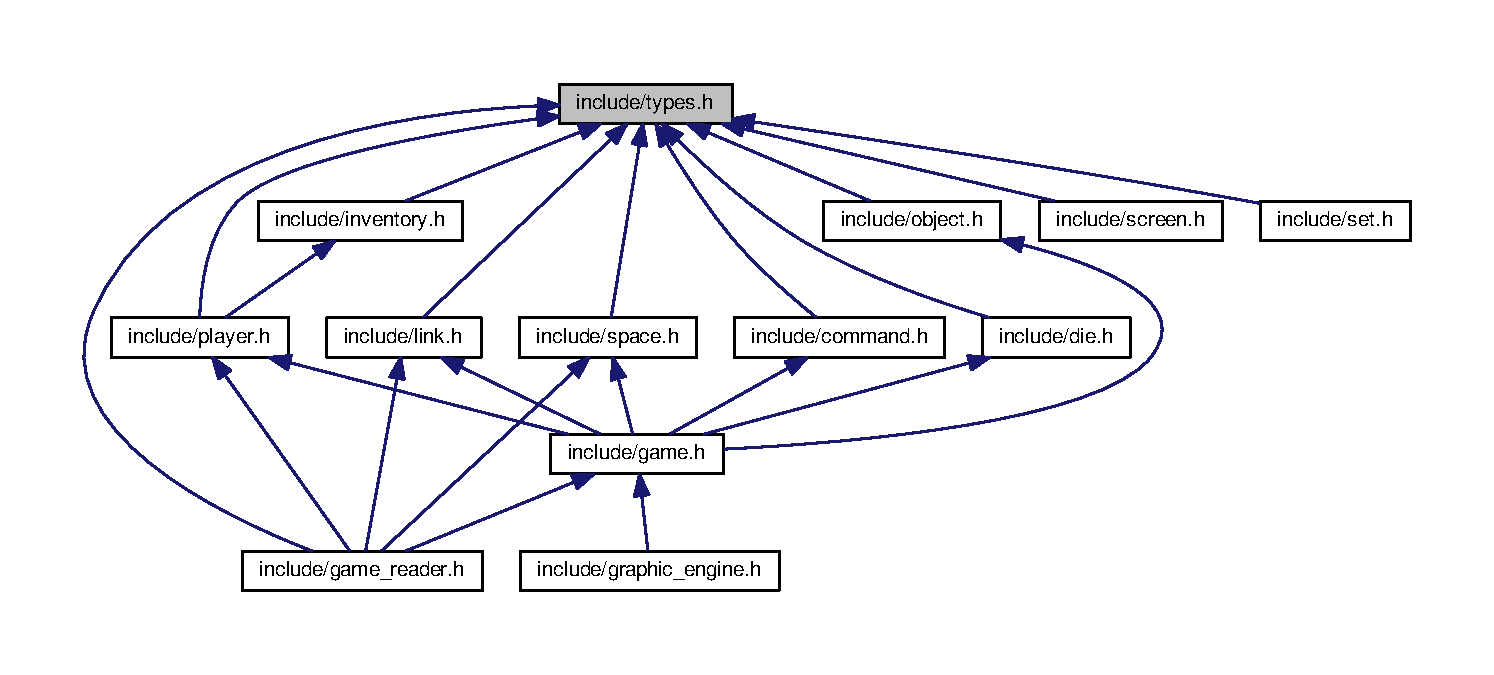
\includegraphics[width=350pt]{types_8h__dep__incl}
\end{center}
\end{figure}
\subsection*{Macros}
\begin{DoxyCompactItemize}
\item 
\#define \hyperlink{types_8h_a9990950cd307079021e49d95eae07c60}{M\+A\+X\+\_\+\+C\+H\+E\+C\+K\+\_\+C}~75
\item 
\#define \hyperlink{types_8h_ae41569a4c2560714ec2b9feb28919682}{M\+A\+X\+\_\+\+C\+H\+E\+C\+K\+\_\+R}~3
\item 
\#define \hyperlink{types_8h_ab6eb8120e52efba3f4f3e27bd22909be}{M\+A\+X\+\_\+\+G\+D\+E\+S\+C\+\_\+C}~8
\item 
\#define \hyperlink{types_8h_a757649d8782333030568604676c4b0a0}{M\+A\+X\+\_\+\+G\+D\+E\+S\+C\+\_\+R}~3
\item 
\#define \hyperlink{types_8h_ac7c0207aa5a0e10d378be03b68041350}{M\+A\+X\+\_\+\+N\+A\+ME}~128
\item 
\#define \hyperlink{types_8h_a92ed8507d1cd2331ad09275c5c4c1c89}{W\+O\+R\+D\+\_\+\+S\+I\+ZE}~1000
\item 
\#define \hyperlink{types_8h_a642e16f35aa1e585c25e405ede76e115}{N\+O\+\_\+\+ID}~-\/1
\item 
\#define \hyperlink{types_8h_a33bfc1f995233887a0414369c36936b8}{N\+O\+T\+\_\+\+F\+O\+U\+ND}~-\/1
\item 
\#define \hyperlink{types_8h_a200b0626733605ecbd9b7ecb79a8c3a3}{S\+E\+T\+\_\+\+M\+A\+X\+\_\+\+I\+DS}~5
\item 
\#define \hyperlink{types_8h_a5f54fd55f983a2e33ce076cd9f587e82}{M\+A\+X\+\_\+\+S\+P\+A\+C\+ES}~100
\item 
\#define \hyperlink{types_8h_a1c346c944e8204fd06dc057393c7c96d}{M\+A\+X\+\_\+\+P\+L\+A\+Y\+E\+RS}~10
\item 
\#define \hyperlink{types_8h_acdc7844fbd4d45737d4aa56834d37829}{M\+A\+X\+\_\+\+O\+B\+J\+E\+C\+TS}~10
\item 
\#define \hyperlink{types_8h_a1248a564e12a816260b44340c9adedfa}{M\+A\+X\+\_\+\+D\+I\+ES}~10
\item 
\#define \hyperlink{types_8h_a660ed1ec8604982002a0d6eced0e0367}{M\+A\+X\+\_\+\+L\+I\+N\+KS}~50
\item 
\#define \hyperlink{types_8h_aa653c0eca99802a09fd9560f28a9b1c1}{M\+A\+X\+\_\+\+T\+A\+GS}~10
\item 
\#define \hyperlink{types_8h_a042ea1e5827a34a330a514290d626e02}{I\+D\+\_\+\+R\+A\+N\+GE}~1000
\item 
\#define \hyperlink{types_8h_af7ffcb470c09612da2829bafd749f98b}{S\+P\+A\+C\+E\+\_\+\+B\+A\+S\+E\+\_\+\+ID}~0000
\item 
\#define \hyperlink{types_8h_a2e035ea155675521eca28608d200a331}{P\+L\+A\+Y\+E\+R\+\_\+\+B\+A\+S\+E\+\_\+\+ID}~1000
\item 
\#define \hyperlink{types_8h_aceddbab5216f311ec0397e23b52fd221}{O\+B\+J\+E\+C\+T\+\_\+\+B\+A\+S\+E\+\_\+\+ID}~2000
\item 
\#define \hyperlink{types_8h_a69b4a4796892b3f189ef14bc8f0b2ab3}{D\+I\+E\+\_\+\+B\+A\+S\+E\+\_\+\+ID}~3000
\item 
\#define \hyperlink{types_8h_a2327fd07bc842e2ba72a700ffa2b6fbc}{L\+I\+N\+K\+\_\+\+B\+A\+S\+E\+\_\+\+ID}~4000
\end{DoxyCompactItemize}
\subsection*{Typedefs}
\begin{DoxyCompactItemize}
\item 
typedef long \hyperlink{types_8h_a845e604fb28f7e3d97549da3448149d3}{Id}\hypertarget{types_8h_a845e604fb28f7e3d97549da3448149d3}{}\label{types_8h_a845e604fb28f7e3d97549da3448149d3}

\begin{DoxyCompactList}\small\item\em Id (to store Ids of objects, players, etc) \end{DoxyCompactList}\end{DoxyCompactItemize}
\subsection*{Enumerations}
\begin{DoxyCompactItemize}
\item 
enum \hyperlink{types_8h_a3e5b8192e7d9ffaf3542f1210aec18dd}{B\+O\+OL} \{ \hyperlink{types_8h_a3e5b8192e7d9ffaf3542f1210aec18ddaa1e095cc966dbecf6a0d8aad75348d1a}{F\+A\+L\+SE}, 
\hyperlink{types_8h_a3e5b8192e7d9ffaf3542f1210aec18ddaa82764c3079aea4e60c80e45befbb839}{T\+R\+UE}
 \}\begin{DoxyCompactList}\small\item\em Boolean (to store boolean values that are or not) \end{DoxyCompactList}
\item 
enum \hyperlink{types_8h_a32c27cc471df37f4fc818d65de0a56c4}{S\+T\+A\+T\+US} \{ \hyperlink{types_8h_a32c27cc471df37f4fc818d65de0a56c4a2fd6f336d08340583bd620a7f5694c90}{E\+R\+R\+OR}, 
\hyperlink{types_8h_a32c27cc471df37f4fc818d65de0a56c4a2bc49ec37d6a5715dd23e85f1ff5bb59}{OK}
 \}\begin{DoxyCompactList}\small\item\em Status (to store all the executions, if correct or not) \end{DoxyCompactList}
\item 
enum \hyperlink{types_8h_a92dd10a73cd77d692dff6c0b2af222f9}{T\+\_\+\+Command} \{ \\*
\hyperlink{types_8h_a92dd10a73cd77d692dff6c0b2af222f9a785693a1d550a18688638e9124af41d0}{N\+O\+\_\+\+C\+MD} = -\/1, 
\hyperlink{types_8h_a92dd10a73cd77d692dff6c0b2af222f9a6ce26a62afab55d7606ad4e92428b30c}{U\+N\+K\+N\+O\+WN}, 
\hyperlink{types_8h_a92dd10a73cd77d692dff6c0b2af222f9a7a10b5d68d31711288e1fe0fa17dbf4f}{E\+X\+IT}, 
\hyperlink{types_8h_a92dd10a73cd77d692dff6c0b2af222f9ac241aecbe2e3eba2f42ce28777f6ab65}{F\+O\+L\+L\+O\+W\+I\+NG}, 
\\*
\hyperlink{types_8h_a92dd10a73cd77d692dff6c0b2af222f9ad9600a436d5cc272dfd53f6c45fdeca4}{P\+R\+E\+V\+I\+O\+US}, 
\hyperlink{types_8h_a92dd10a73cd77d692dff6c0b2af222f9a362b5ae0e519db264a4b2607d37d2a7e}{G\+R\+A\+SP}, 
\hyperlink{types_8h_a92dd10a73cd77d692dff6c0b2af222f9a8b0b0025af76a3d8f0b7b1d4758e51a6}{D\+R\+OP}, 
\hyperlink{types_8h_a92dd10a73cd77d692dff6c0b2af222f9abc5a79c786d2b239440dd3b92c402ef4}{T\+H\+R\+OW}, 
\\*
\hyperlink{types_8h_a92dd10a73cd77d692dff6c0b2af222f9aec8379af7490bb9eaaf579cf17876f38}{R\+I\+G\+HT}, 
\hyperlink{types_8h_a92dd10a73cd77d692dff6c0b2af222f9adb45120aafd37a973140edee24708065}{L\+E\+FT}, 
\hyperlink{types_8h_a92dd10a73cd77d692dff6c0b2af222f9aed3ef32890b6da0919b57254c5206c62}{M\+O\+VE}, 
{\bfseries C\+H\+E\+CK}
 \}\begin{DoxyCompactList}\small\item\em Command enumeration (to be used on command.\+c. \end{DoxyCompactList}
\item 
enum \hyperlink{types_8h_aa268a41a13430b18e933ed40207178d0}{D\+I\+R\+E\+C\+T\+I\+ON} \{ \\*
\hyperlink{types_8h_aa268a41a13430b18e933ed40207178d0a0f886785b600b91048fcdc434c6b4a8e}{E\+RR} = -\/1, 
\hyperlink{types_8h_aa268a41a13430b18e933ed40207178d0a2c63acbe79d9f41ba6bb7766e9c37702}{N}, 
\hyperlink{types_8h_aa268a41a13430b18e933ed40207178d0ab722ceeb601c72cd78fbd35f3581fdf7}{W}, 
\hyperlink{types_8h_aa268a41a13430b18e933ed40207178d0af1ce01387d2348f8b858721a7db81670}{S}, 
\\*
\hyperlink{types_8h_aa268a41a13430b18e933ed40207178d0ab199e021998d49b1f09338d8b9b18ecb}{E}
 \}\begin{DoxyCompactList}\small\item\em Direction (to be used when moving through the board) \end{DoxyCompactList}
\item 
enum \hyperlink{types_8h_ab0ce7873e5a1bd8bc18fafaaed449b24}{L\+I\+N\+K\+\_\+\+S\+T\+A\+T\+US} \{ \hyperlink{types_8h_ab0ce7873e5a1bd8bc18fafaaed449b24a0e0143636c29971736eab47415868eae}{O\+P\+EN} = 0, 
\hyperlink{types_8h_ab0ce7873e5a1bd8bc18fafaaed449b24a929f0327e17604ce9713b2a6117bd603}{C\+L\+O\+S\+ED} = 1
 \}\begin{DoxyCompactList}\small\item\em L\+I\+N\+K\+\_\+\+S\+T\+A\+T\+US enumeration (to be used on links) \end{DoxyCompactList}
\item 
enum \hyperlink{types_8h_af90824509586333cf45ce757d2711ce3}{C\+O\+L\+OR} \{ \\*
\hyperlink{types_8h_af90824509586333cf45ce757d2711ce3af77fb67151d0c18d397069ad8c271ba3}{B\+L\+A\+CK}, 
\hyperlink{types_8h_af90824509586333cf45ce757d2711ce3af80f9a890089d211842d59625e561f88}{R\+ED}, 
\hyperlink{types_8h_af90824509586333cf45ce757d2711ce3aa60bd322f93178d68184e30e162571ca}{G\+R\+E\+EN}, 
\hyperlink{types_8h_af90824509586333cf45ce757d2711ce3ae735a848bf82163a19236ead1c3ef2d2}{Y\+E\+L\+L\+OW}, 
\\*
\hyperlink{types_8h_af90824509586333cf45ce757d2711ce3a35d6719cb4d7577c031b3d79057a1b79}{B\+L\+UE}, 
\hyperlink{types_8h_af90824509586333cf45ce757d2711ce3a2772ad7cd64f03c2aed60f91c69fa69d}{P\+U\+R\+P\+LE}, 
\hyperlink{types_8h_af90824509586333cf45ce757d2711ce3aafe71cad474c15ce63b300c470eef8cc}{C\+Y\+AN}, 
\hyperlink{types_8h_af90824509586333cf45ce757d2711ce3a283fc479650da98250635b9c3c0e7e50}{W\+H\+I\+TE}
 \}\begin{DoxyCompactList}\small\item\em C\+O\+L\+OR enumeration (to be used when painting the graphic engine) \end{DoxyCompactList}
\item 
enum \hyperlink{types_8h_a781b03b8eb5f35cf89f3c931ffa26e35}{T\+AG} \{ \\*
\hyperlink{types_8h_a781b03b8eb5f35cf89f3c931ffa26e35a33ca3be4d5e7ce4b0ef99a4819746d6c}{N\+O\+\_\+\+T\+AG} = 0, 
\hyperlink{types_8h_a781b03b8eb5f35cf89f3c931ffa26e35abb22a6fcb7f208995b092f12d388786c}{V\+I\+S\+I\+B\+LE}, 
\hyperlink{types_8h_a781b03b8eb5f35cf89f3c931ffa26e35a9d86737eb7a3c269abe82f3024c407eb}{M\+O\+V\+A\+B\+LE}, 
\hyperlink{types_8h_a781b03b8eb5f35cf89f3c931ffa26e35ae2ce5b938a5d96737d97e2c19658e494}{M\+O\+V\+ED}, 
\\*
\hyperlink{types_8h_a781b03b8eb5f35cf89f3c931ffa26e35a41ae0a505430bf564b119bc82db7592d}{H\+I\+D\+D\+EN}, 
\hyperlink{types_8h_a781b03b8eb5f35cf89f3c931ffa26e35a8686d5818408054e50d4da4b0860ccba}{C\+A\+N\+\_\+\+G\+L\+OW}, 
\hyperlink{types_8h_a781b03b8eb5f35cf89f3c931ffa26e35ae02a1c2718542e66c1d67adcb098a9b9}{G\+L\+O\+W\+I\+NG}, 
\hyperlink{types_8h_a781b03b8eb5f35cf89f3c931ffa26e35a7bf039b3239c63e77c09bf900757b081}{I\+S\+\_\+\+K\+EY}
 \}\begin{DoxyCompactList}\small\item\em T\+AG enumeration (to be used when asigning propierties to objects) \end{DoxyCompactList}
\end{DoxyCompactItemize}


\subsection{Detailed Description}
It defines common types. 

\begin{DoxyAuthor}{Author}
Profesores P\+P\+R\+OG 
\end{DoxyAuthor}
\begin{DoxyVersion}{Version}
1.\+0 
\end{DoxyVersion}
\begin{DoxyDate}{Date}
13-\/01-\/2015 
\end{DoxyDate}
\begin{DoxyCopyright}{Copyright}
G\+NU Public License 
\end{DoxyCopyright}


\subsection{Macro Definition Documentation}
\index{types.\+h@{types.\+h}!D\+I\+E\+\_\+\+B\+A\+S\+E\+\_\+\+ID@{D\+I\+E\+\_\+\+B\+A\+S\+E\+\_\+\+ID}}
\index{D\+I\+E\+\_\+\+B\+A\+S\+E\+\_\+\+ID@{D\+I\+E\+\_\+\+B\+A\+S\+E\+\_\+\+ID}!types.\+h@{types.\+h}}
\subsubsection[{\texorpdfstring{D\+I\+E\+\_\+\+B\+A\+S\+E\+\_\+\+ID}{DIE_BASE_ID}}]{\setlength{\rightskip}{0pt plus 5cm}\#define D\+I\+E\+\_\+\+B\+A\+S\+E\+\_\+\+ID~3000}\hypertarget{types_8h_a69b4a4796892b3f189ef14bc8f0b2ab3}{}\label{types_8h_a69b4a4796892b3f189ef14bc8f0b2ab3}
Marks where the Dies Ids start \index{types.\+h@{types.\+h}!I\+D\+\_\+\+R\+A\+N\+GE@{I\+D\+\_\+\+R\+A\+N\+GE}}
\index{I\+D\+\_\+\+R\+A\+N\+GE@{I\+D\+\_\+\+R\+A\+N\+GE}!types.\+h@{types.\+h}}
\subsubsection[{\texorpdfstring{I\+D\+\_\+\+R\+A\+N\+GE}{ID_RANGE}}]{\setlength{\rightskip}{0pt plus 5cm}\#define I\+D\+\_\+\+R\+A\+N\+GE~1000}\hypertarget{types_8h_a042ea1e5827a34a330a514290d626e02}{}\label{types_8h_a042ea1e5827a34a330a514290d626e02}
Used to define the maximum amount of elements from each type we can manage \index{types.\+h@{types.\+h}!L\+I\+N\+K\+\_\+\+B\+A\+S\+E\+\_\+\+ID@{L\+I\+N\+K\+\_\+\+B\+A\+S\+E\+\_\+\+ID}}
\index{L\+I\+N\+K\+\_\+\+B\+A\+S\+E\+\_\+\+ID@{L\+I\+N\+K\+\_\+\+B\+A\+S\+E\+\_\+\+ID}!types.\+h@{types.\+h}}
\subsubsection[{\texorpdfstring{L\+I\+N\+K\+\_\+\+B\+A\+S\+E\+\_\+\+ID}{LINK_BASE_ID}}]{\setlength{\rightskip}{0pt plus 5cm}\#define L\+I\+N\+K\+\_\+\+B\+A\+S\+E\+\_\+\+ID~4000}\hypertarget{types_8h_a2327fd07bc842e2ba72a700ffa2b6fbc}{}\label{types_8h_a2327fd07bc842e2ba72a700ffa2b6fbc}
Marks where the Links Ids start \index{types.\+h@{types.\+h}!M\+A\+X\+\_\+\+C\+H\+E\+C\+K\+\_\+C@{M\+A\+X\+\_\+\+C\+H\+E\+C\+K\+\_\+C}}
\index{M\+A\+X\+\_\+\+C\+H\+E\+C\+K\+\_\+C@{M\+A\+X\+\_\+\+C\+H\+E\+C\+K\+\_\+C}!types.\+h@{types.\+h}}
\subsubsection[{\texorpdfstring{M\+A\+X\+\_\+\+C\+H\+E\+C\+K\+\_\+C}{MAX_CHECK_C}}]{\setlength{\rightskip}{0pt plus 5cm}\#define M\+A\+X\+\_\+\+C\+H\+E\+C\+K\+\_\+C~75}\hypertarget{types_8h_a9990950cd307079021e49d95eae07c60}{}\label{types_8h_a9990950cd307079021e49d95eae07c60}
Maximum columns of the check field \index{types.\+h@{types.\+h}!M\+A\+X\+\_\+\+C\+H\+E\+C\+K\+\_\+R@{M\+A\+X\+\_\+\+C\+H\+E\+C\+K\+\_\+R}}
\index{M\+A\+X\+\_\+\+C\+H\+E\+C\+K\+\_\+R@{M\+A\+X\+\_\+\+C\+H\+E\+C\+K\+\_\+R}!types.\+h@{types.\+h}}
\subsubsection[{\texorpdfstring{M\+A\+X\+\_\+\+C\+H\+E\+C\+K\+\_\+R}{MAX_CHECK_R}}]{\setlength{\rightskip}{0pt plus 5cm}\#define M\+A\+X\+\_\+\+C\+H\+E\+C\+K\+\_\+R~3}\hypertarget{types_8h_ae41569a4c2560714ec2b9feb28919682}{}\label{types_8h_ae41569a4c2560714ec2b9feb28919682}
Maximum rows of the check field \index{types.\+h@{types.\+h}!M\+A\+X\+\_\+\+D\+I\+ES@{M\+A\+X\+\_\+\+D\+I\+ES}}
\index{M\+A\+X\+\_\+\+D\+I\+ES@{M\+A\+X\+\_\+\+D\+I\+ES}!types.\+h@{types.\+h}}
\subsubsection[{\texorpdfstring{M\+A\+X\+\_\+\+D\+I\+ES}{MAX_DIES}}]{\setlength{\rightskip}{0pt plus 5cm}\#define M\+A\+X\+\_\+\+D\+I\+ES~10}\hypertarget{types_8h_a1248a564e12a816260b44340c9adedfa}{}\label{types_8h_a1248a564e12a816260b44340c9adedfa}
Maximum number of dies a game is prepared to store \index{types.\+h@{types.\+h}!M\+A\+X\+\_\+\+G\+D\+E\+S\+C\+\_\+C@{M\+A\+X\+\_\+\+G\+D\+E\+S\+C\+\_\+C}}
\index{M\+A\+X\+\_\+\+G\+D\+E\+S\+C\+\_\+C@{M\+A\+X\+\_\+\+G\+D\+E\+S\+C\+\_\+C}!types.\+h@{types.\+h}}
\subsubsection[{\texorpdfstring{M\+A\+X\+\_\+\+G\+D\+E\+S\+C\+\_\+C}{MAX_GDESC_C}}]{\setlength{\rightskip}{0pt plus 5cm}\#define M\+A\+X\+\_\+\+G\+D\+E\+S\+C\+\_\+C~8}\hypertarget{types_8h_ab6eb8120e52efba3f4f3e27bd22909be}{}\label{types_8h_ab6eb8120e52efba3f4f3e27bd22909be}
Maximum columns of the graphic description field \index{types.\+h@{types.\+h}!M\+A\+X\+\_\+\+G\+D\+E\+S\+C\+\_\+R@{M\+A\+X\+\_\+\+G\+D\+E\+S\+C\+\_\+R}}
\index{M\+A\+X\+\_\+\+G\+D\+E\+S\+C\+\_\+R@{M\+A\+X\+\_\+\+G\+D\+E\+S\+C\+\_\+R}!types.\+h@{types.\+h}}
\subsubsection[{\texorpdfstring{M\+A\+X\+\_\+\+G\+D\+E\+S\+C\+\_\+R}{MAX_GDESC_R}}]{\setlength{\rightskip}{0pt plus 5cm}\#define M\+A\+X\+\_\+\+G\+D\+E\+S\+C\+\_\+R~3}\hypertarget{types_8h_a757649d8782333030568604676c4b0a0}{}\label{types_8h_a757649d8782333030568604676c4b0a0}
Maximum rows of the graphic description field \index{types.\+h@{types.\+h}!M\+A\+X\+\_\+\+L\+I\+N\+KS@{M\+A\+X\+\_\+\+L\+I\+N\+KS}}
\index{M\+A\+X\+\_\+\+L\+I\+N\+KS@{M\+A\+X\+\_\+\+L\+I\+N\+KS}!types.\+h@{types.\+h}}
\subsubsection[{\texorpdfstring{M\+A\+X\+\_\+\+L\+I\+N\+KS}{MAX_LINKS}}]{\setlength{\rightskip}{0pt plus 5cm}\#define M\+A\+X\+\_\+\+L\+I\+N\+KS~50}\hypertarget{types_8h_a660ed1ec8604982002a0d6eced0e0367}{}\label{types_8h_a660ed1ec8604982002a0d6eced0e0367}
Maximum number of links a game is prepared to store \index{types.\+h@{types.\+h}!M\+A\+X\+\_\+\+N\+A\+ME@{M\+A\+X\+\_\+\+N\+A\+ME}}
\index{M\+A\+X\+\_\+\+N\+A\+ME@{M\+A\+X\+\_\+\+N\+A\+ME}!types.\+h@{types.\+h}}
\subsubsection[{\texorpdfstring{M\+A\+X\+\_\+\+N\+A\+ME}{MAX_NAME}}]{\setlength{\rightskip}{0pt plus 5cm}\#define M\+A\+X\+\_\+\+N\+A\+ME~128}\hypertarget{types_8h_ac7c0207aa5a0e10d378be03b68041350}{}\label{types_8h_ac7c0207aa5a0e10d378be03b68041350}
Maximum characters of a link name \index{types.\+h@{types.\+h}!M\+A\+X\+\_\+\+O\+B\+J\+E\+C\+TS@{M\+A\+X\+\_\+\+O\+B\+J\+E\+C\+TS}}
\index{M\+A\+X\+\_\+\+O\+B\+J\+E\+C\+TS@{M\+A\+X\+\_\+\+O\+B\+J\+E\+C\+TS}!types.\+h@{types.\+h}}
\subsubsection[{\texorpdfstring{M\+A\+X\+\_\+\+O\+B\+J\+E\+C\+TS}{MAX_OBJECTS}}]{\setlength{\rightskip}{0pt plus 5cm}\#define M\+A\+X\+\_\+\+O\+B\+J\+E\+C\+TS~10}\hypertarget{types_8h_acdc7844fbd4d45737d4aa56834d37829}{}\label{types_8h_acdc7844fbd4d45737d4aa56834d37829}
Maximum number of objects a game is prepared to store \index{types.\+h@{types.\+h}!M\+A\+X\+\_\+\+P\+L\+A\+Y\+E\+RS@{M\+A\+X\+\_\+\+P\+L\+A\+Y\+E\+RS}}
\index{M\+A\+X\+\_\+\+P\+L\+A\+Y\+E\+RS@{M\+A\+X\+\_\+\+P\+L\+A\+Y\+E\+RS}!types.\+h@{types.\+h}}
\subsubsection[{\texorpdfstring{M\+A\+X\+\_\+\+P\+L\+A\+Y\+E\+RS}{MAX_PLAYERS}}]{\setlength{\rightskip}{0pt plus 5cm}\#define M\+A\+X\+\_\+\+P\+L\+A\+Y\+E\+RS~10}\hypertarget{types_8h_a1c346c944e8204fd06dc057393c7c96d}{}\label{types_8h_a1c346c944e8204fd06dc057393c7c96d}
Maximum number of players a game is prepared to store \index{types.\+h@{types.\+h}!M\+A\+X\+\_\+\+S\+P\+A\+C\+ES@{M\+A\+X\+\_\+\+S\+P\+A\+C\+ES}}
\index{M\+A\+X\+\_\+\+S\+P\+A\+C\+ES@{M\+A\+X\+\_\+\+S\+P\+A\+C\+ES}!types.\+h@{types.\+h}}
\subsubsection[{\texorpdfstring{M\+A\+X\+\_\+\+S\+P\+A\+C\+ES}{MAX_SPACES}}]{\setlength{\rightskip}{0pt plus 5cm}\#define M\+A\+X\+\_\+\+S\+P\+A\+C\+ES~100}\hypertarget{types_8h_a5f54fd55f983a2e33ce076cd9f587e82}{}\label{types_8h_a5f54fd55f983a2e33ce076cd9f587e82}
Maximum number of spaces a game is prepared to store \index{types.\+h@{types.\+h}!M\+A\+X\+\_\+\+T\+A\+GS@{M\+A\+X\+\_\+\+T\+A\+GS}}
\index{M\+A\+X\+\_\+\+T\+A\+GS@{M\+A\+X\+\_\+\+T\+A\+GS}!types.\+h@{types.\+h}}
\subsubsection[{\texorpdfstring{M\+A\+X\+\_\+\+T\+A\+GS}{MAX_TAGS}}]{\setlength{\rightskip}{0pt plus 5cm}\#define M\+A\+X\+\_\+\+T\+A\+GS~10}\hypertarget{types_8h_aa653c0eca99802a09fd9560f28a9b1c1}{}\label{types_8h_aa653c0eca99802a09fd9560f28a9b1c1}
Maximun number of tags an object can have \index{types.\+h@{types.\+h}!N\+O\+\_\+\+ID@{N\+O\+\_\+\+ID}}
\index{N\+O\+\_\+\+ID@{N\+O\+\_\+\+ID}!types.\+h@{types.\+h}}
\subsubsection[{\texorpdfstring{N\+O\+\_\+\+ID}{NO_ID}}]{\setlength{\rightskip}{0pt plus 5cm}\#define N\+O\+\_\+\+ID~-\/1}\hypertarget{types_8h_a642e16f35aa1e585c25e405ede76e115}{}\label{types_8h_a642e16f35aa1e585c25e405ede76e115}
Default Id used when there is no Id or something works as it shouldn\textquotesingle{}t \index{types.\+h@{types.\+h}!N\+O\+T\+\_\+\+F\+O\+U\+ND@{N\+O\+T\+\_\+\+F\+O\+U\+ND}}
\index{N\+O\+T\+\_\+\+F\+O\+U\+ND@{N\+O\+T\+\_\+\+F\+O\+U\+ND}!types.\+h@{types.\+h}}
\subsubsection[{\texorpdfstring{N\+O\+T\+\_\+\+F\+O\+U\+ND}{NOT_FOUND}}]{\setlength{\rightskip}{0pt plus 5cm}\#define N\+O\+T\+\_\+\+F\+O\+U\+ND~-\/1}\hypertarget{types_8h_a33bfc1f995233887a0414369c36936b8}{}\label{types_8h_a33bfc1f995233887a0414369c36936b8}
Used when a set doesnt found the given Id position \index{types.\+h@{types.\+h}!O\+B\+J\+E\+C\+T\+\_\+\+B\+A\+S\+E\+\_\+\+ID@{O\+B\+J\+E\+C\+T\+\_\+\+B\+A\+S\+E\+\_\+\+ID}}
\index{O\+B\+J\+E\+C\+T\+\_\+\+B\+A\+S\+E\+\_\+\+ID@{O\+B\+J\+E\+C\+T\+\_\+\+B\+A\+S\+E\+\_\+\+ID}!types.\+h@{types.\+h}}
\subsubsection[{\texorpdfstring{O\+B\+J\+E\+C\+T\+\_\+\+B\+A\+S\+E\+\_\+\+ID}{OBJECT_BASE_ID}}]{\setlength{\rightskip}{0pt plus 5cm}\#define O\+B\+J\+E\+C\+T\+\_\+\+B\+A\+S\+E\+\_\+\+ID~2000}\hypertarget{types_8h_aceddbab5216f311ec0397e23b52fd221}{}\label{types_8h_aceddbab5216f311ec0397e23b52fd221}
Marks where the Objects Ids start \index{types.\+h@{types.\+h}!P\+L\+A\+Y\+E\+R\+\_\+\+B\+A\+S\+E\+\_\+\+ID@{P\+L\+A\+Y\+E\+R\+\_\+\+B\+A\+S\+E\+\_\+\+ID}}
\index{P\+L\+A\+Y\+E\+R\+\_\+\+B\+A\+S\+E\+\_\+\+ID@{P\+L\+A\+Y\+E\+R\+\_\+\+B\+A\+S\+E\+\_\+\+ID}!types.\+h@{types.\+h}}
\subsubsection[{\texorpdfstring{P\+L\+A\+Y\+E\+R\+\_\+\+B\+A\+S\+E\+\_\+\+ID}{PLAYER_BASE_ID}}]{\setlength{\rightskip}{0pt plus 5cm}\#define P\+L\+A\+Y\+E\+R\+\_\+\+B\+A\+S\+E\+\_\+\+ID~1000}\hypertarget{types_8h_a2e035ea155675521eca28608d200a331}{}\label{types_8h_a2e035ea155675521eca28608d200a331}
Marks where the Players Ids start \index{types.\+h@{types.\+h}!S\+E\+T\+\_\+\+M\+A\+X\+\_\+\+I\+DS@{S\+E\+T\+\_\+\+M\+A\+X\+\_\+\+I\+DS}}
\index{S\+E\+T\+\_\+\+M\+A\+X\+\_\+\+I\+DS@{S\+E\+T\+\_\+\+M\+A\+X\+\_\+\+I\+DS}!types.\+h@{types.\+h}}
\subsubsection[{\texorpdfstring{S\+E\+T\+\_\+\+M\+A\+X\+\_\+\+I\+DS}{SET_MAX_IDS}}]{\setlength{\rightskip}{0pt plus 5cm}\#define S\+E\+T\+\_\+\+M\+A\+X\+\_\+\+I\+DS~5}\hypertarget{types_8h_a200b0626733605ecbd9b7ecb79a8c3a3}{}\label{types_8h_a200b0626733605ecbd9b7ecb79a8c3a3}
Maximum number of Ids a set can store \index{types.\+h@{types.\+h}!S\+P\+A\+C\+E\+\_\+\+B\+A\+S\+E\+\_\+\+ID@{S\+P\+A\+C\+E\+\_\+\+B\+A\+S\+E\+\_\+\+ID}}
\index{S\+P\+A\+C\+E\+\_\+\+B\+A\+S\+E\+\_\+\+ID@{S\+P\+A\+C\+E\+\_\+\+B\+A\+S\+E\+\_\+\+ID}!types.\+h@{types.\+h}}
\subsubsection[{\texorpdfstring{S\+P\+A\+C\+E\+\_\+\+B\+A\+S\+E\+\_\+\+ID}{SPACE_BASE_ID}}]{\setlength{\rightskip}{0pt plus 5cm}\#define S\+P\+A\+C\+E\+\_\+\+B\+A\+S\+E\+\_\+\+ID~0000}\hypertarget{types_8h_af7ffcb470c09612da2829bafd749f98b}{}\label{types_8h_af7ffcb470c09612da2829bafd749f98b}
Marks where the Spaces Ids start \index{types.\+h@{types.\+h}!W\+O\+R\+D\+\_\+\+S\+I\+ZE@{W\+O\+R\+D\+\_\+\+S\+I\+ZE}}
\index{W\+O\+R\+D\+\_\+\+S\+I\+ZE@{W\+O\+R\+D\+\_\+\+S\+I\+ZE}!types.\+h@{types.\+h}}
\subsubsection[{\texorpdfstring{W\+O\+R\+D\+\_\+\+S\+I\+ZE}{WORD_SIZE}}]{\setlength{\rightskip}{0pt plus 5cm}\#define W\+O\+R\+D\+\_\+\+S\+I\+ZE~1000}\hypertarget{types_8h_a92ed8507d1cd2331ad09275c5c4c1c89}{}\label{types_8h_a92ed8507d1cd2331ad09275c5c4c1c89}
Maximum size of some of the names (players, objects and else) 

\subsection{Enumeration Type Documentation}
\index{types.\+h@{types.\+h}!B\+O\+OL@{B\+O\+OL}}
\index{B\+O\+OL@{B\+O\+OL}!types.\+h@{types.\+h}}
\subsubsection[{\texorpdfstring{B\+O\+OL}{BOOL}}]{\setlength{\rightskip}{0pt plus 5cm}enum {\bf B\+O\+OL}}\hypertarget{types_8h_a3e5b8192e7d9ffaf3542f1210aec18dd}{}\label{types_8h_a3e5b8192e7d9ffaf3542f1210aec18dd}


Boolean (to store boolean values that are or not) 

\begin{Desc}
\item[Enumerator]\par
\begin{description}
\index{F\+A\+L\+SE@{F\+A\+L\+SE}!types.\+h@{types.\+h}}\index{types.\+h@{types.\+h}!F\+A\+L\+SE@{F\+A\+L\+SE}}\item[{\em 
F\+A\+L\+SE\hypertarget{types_8h_a3e5b8192e7d9ffaf3542f1210aec18ddaa1e095cc966dbecf6a0d8aad75348d1a}{}\label{types_8h_a3e5b8192e7d9ffaf3542f1210aec18ddaa1e095cc966dbecf6a0d8aad75348d1a}
}]If the condition is not fullfilled \index{T\+R\+UE@{T\+R\+UE}!types.\+h@{types.\+h}}\index{types.\+h@{types.\+h}!T\+R\+UE@{T\+R\+UE}}\item[{\em 
T\+R\+UE\hypertarget{types_8h_a3e5b8192e7d9ffaf3542f1210aec18ddaa82764c3079aea4e60c80e45befbb839}{}\label{types_8h_a3e5b8192e7d9ffaf3542f1210aec18ddaa82764c3079aea4e60c80e45befbb839}
}]If the condition is correct and real \end{description}
\end{Desc}
\index{types.\+h@{types.\+h}!C\+O\+L\+OR@{C\+O\+L\+OR}}
\index{C\+O\+L\+OR@{C\+O\+L\+OR}!types.\+h@{types.\+h}}
\subsubsection[{\texorpdfstring{C\+O\+L\+OR}{COLOR}}]{\setlength{\rightskip}{0pt plus 5cm}enum {\bf C\+O\+L\+OR}}\hypertarget{types_8h_af90824509586333cf45ce757d2711ce3}{}\label{types_8h_af90824509586333cf45ce757d2711ce3}


C\+O\+L\+OR enumeration (to be used when painting the graphic engine) 

\begin{Desc}
\item[Enumerator]\par
\begin{description}
\index{B\+L\+A\+CK@{B\+L\+A\+CK}!types.\+h@{types.\+h}}\index{types.\+h@{types.\+h}!B\+L\+A\+CK@{B\+L\+A\+CK}}\item[{\em 
B\+L\+A\+CK\hypertarget{types_8h_af90824509586333cf45ce757d2711ce3af77fb67151d0c18d397069ad8c271ba3}{}\label{types_8h_af90824509586333cf45ce757d2711ce3af77fb67151d0c18d397069ad8c271ba3}
}]B\+L\+A\+CK C\+O\+L\+OR \index{R\+ED@{R\+ED}!types.\+h@{types.\+h}}\index{types.\+h@{types.\+h}!R\+ED@{R\+ED}}\item[{\em 
R\+ED\hypertarget{types_8h_af90824509586333cf45ce757d2711ce3af80f9a890089d211842d59625e561f88}{}\label{types_8h_af90824509586333cf45ce757d2711ce3af80f9a890089d211842d59625e561f88}
}]R\+ED C\+O\+L\+OR \index{G\+R\+E\+EN@{G\+R\+E\+EN}!types.\+h@{types.\+h}}\index{types.\+h@{types.\+h}!G\+R\+E\+EN@{G\+R\+E\+EN}}\item[{\em 
G\+R\+E\+EN\hypertarget{types_8h_af90824509586333cf45ce757d2711ce3aa60bd322f93178d68184e30e162571ca}{}\label{types_8h_af90824509586333cf45ce757d2711ce3aa60bd322f93178d68184e30e162571ca}
}]G\+R\+E\+EN C\+O\+L\+OR \index{Y\+E\+L\+L\+OW@{Y\+E\+L\+L\+OW}!types.\+h@{types.\+h}}\index{types.\+h@{types.\+h}!Y\+E\+L\+L\+OW@{Y\+E\+L\+L\+OW}}\item[{\em 
Y\+E\+L\+L\+OW\hypertarget{types_8h_af90824509586333cf45ce757d2711ce3ae735a848bf82163a19236ead1c3ef2d2}{}\label{types_8h_af90824509586333cf45ce757d2711ce3ae735a848bf82163a19236ead1c3ef2d2}
}]Y\+E\+L\+L\+OW C\+O\+L\+OR \index{B\+L\+UE@{B\+L\+UE}!types.\+h@{types.\+h}}\index{types.\+h@{types.\+h}!B\+L\+UE@{B\+L\+UE}}\item[{\em 
B\+L\+UE\hypertarget{types_8h_af90824509586333cf45ce757d2711ce3a35d6719cb4d7577c031b3d79057a1b79}{}\label{types_8h_af90824509586333cf45ce757d2711ce3a35d6719cb4d7577c031b3d79057a1b79}
}]B\+L\+UE C\+O\+L\+OR \index{P\+U\+R\+P\+LE@{P\+U\+R\+P\+LE}!types.\+h@{types.\+h}}\index{types.\+h@{types.\+h}!P\+U\+R\+P\+LE@{P\+U\+R\+P\+LE}}\item[{\em 
P\+U\+R\+P\+LE\hypertarget{types_8h_af90824509586333cf45ce757d2711ce3a2772ad7cd64f03c2aed60f91c69fa69d}{}\label{types_8h_af90824509586333cf45ce757d2711ce3a2772ad7cd64f03c2aed60f91c69fa69d}
}]P\+U\+R\+P\+LE C\+O\+L\+OR \index{C\+Y\+AN@{C\+Y\+AN}!types.\+h@{types.\+h}}\index{types.\+h@{types.\+h}!C\+Y\+AN@{C\+Y\+AN}}\item[{\em 
C\+Y\+AN\hypertarget{types_8h_af90824509586333cf45ce757d2711ce3aafe71cad474c15ce63b300c470eef8cc}{}\label{types_8h_af90824509586333cf45ce757d2711ce3aafe71cad474c15ce63b300c470eef8cc}
}]C\+Y\+AN C\+O\+L\+OR \index{W\+H\+I\+TE@{W\+H\+I\+TE}!types.\+h@{types.\+h}}\index{types.\+h@{types.\+h}!W\+H\+I\+TE@{W\+H\+I\+TE}}\item[{\em 
W\+H\+I\+TE\hypertarget{types_8h_af90824509586333cf45ce757d2711ce3a283fc479650da98250635b9c3c0e7e50}{}\label{types_8h_af90824509586333cf45ce757d2711ce3a283fc479650da98250635b9c3c0e7e50}
}]W\+H\+I\+TE C\+O\+L\+OR \end{description}
\end{Desc}
\index{types.\+h@{types.\+h}!D\+I\+R\+E\+C\+T\+I\+ON@{D\+I\+R\+E\+C\+T\+I\+ON}}
\index{D\+I\+R\+E\+C\+T\+I\+ON@{D\+I\+R\+E\+C\+T\+I\+ON}!types.\+h@{types.\+h}}
\subsubsection[{\texorpdfstring{D\+I\+R\+E\+C\+T\+I\+ON}{DIRECTION}}]{\setlength{\rightskip}{0pt plus 5cm}enum {\bf D\+I\+R\+E\+C\+T\+I\+ON}}\hypertarget{types_8h_aa268a41a13430b18e933ed40207178d0}{}\label{types_8h_aa268a41a13430b18e933ed40207178d0}


Direction (to be used when moving through the board) 

\begin{Desc}
\item[Enumerator]\par
\begin{description}
\index{E\+RR@{E\+RR}!types.\+h@{types.\+h}}\index{types.\+h@{types.\+h}!E\+RR@{E\+RR}}\item[{\em 
E\+RR\hypertarget{types_8h_aa268a41a13430b18e933ed40207178d0a0f886785b600b91048fcdc434c6b4a8e}{}\label{types_8h_aa268a41a13430b18e933ed40207178d0a0f886785b600b91048fcdc434c6b4a8e}
}]If something went wrong \index{N@{N}!types.\+h@{types.\+h}}\index{types.\+h@{types.\+h}!N@{N}}\item[{\em 
N\hypertarget{types_8h_aa268a41a13430b18e933ed40207178d0a2c63acbe79d9f41ba6bb7766e9c37702}{}\label{types_8h_aa268a41a13430b18e933ed40207178d0a2c63acbe79d9f41ba6bb7766e9c37702}
}]When going North \index{W@{W}!types.\+h@{types.\+h}}\index{types.\+h@{types.\+h}!W@{W}}\item[{\em 
W\hypertarget{types_8h_aa268a41a13430b18e933ed40207178d0ab722ceeb601c72cd78fbd35f3581fdf7}{}\label{types_8h_aa268a41a13430b18e933ed40207178d0ab722ceeb601c72cd78fbd35f3581fdf7}
}]When going West \index{S@{S}!types.\+h@{types.\+h}}\index{types.\+h@{types.\+h}!S@{S}}\item[{\em 
S\hypertarget{types_8h_aa268a41a13430b18e933ed40207178d0af1ce01387d2348f8b858721a7db81670}{}\label{types_8h_aa268a41a13430b18e933ed40207178d0af1ce01387d2348f8b858721a7db81670}
}]When going South \index{E@{E}!types.\+h@{types.\+h}}\index{types.\+h@{types.\+h}!E@{E}}\item[{\em 
E\hypertarget{types_8h_aa268a41a13430b18e933ed40207178d0ab199e021998d49b1f09338d8b9b18ecb}{}\label{types_8h_aa268a41a13430b18e933ed40207178d0ab199e021998d49b1f09338d8b9b18ecb}
}]When going East \end{description}
\end{Desc}
\index{types.\+h@{types.\+h}!L\+I\+N\+K\+\_\+\+S\+T\+A\+T\+US@{L\+I\+N\+K\+\_\+\+S\+T\+A\+T\+US}}
\index{L\+I\+N\+K\+\_\+\+S\+T\+A\+T\+US@{L\+I\+N\+K\+\_\+\+S\+T\+A\+T\+US}!types.\+h@{types.\+h}}
\subsubsection[{\texorpdfstring{L\+I\+N\+K\+\_\+\+S\+T\+A\+T\+US}{LINK_STATUS}}]{\setlength{\rightskip}{0pt plus 5cm}enum {\bf L\+I\+N\+K\+\_\+\+S\+T\+A\+T\+US}}\hypertarget{types_8h_ab0ce7873e5a1bd8bc18fafaaed449b24}{}\label{types_8h_ab0ce7873e5a1bd8bc18fafaaed449b24}


L\+I\+N\+K\+\_\+\+S\+T\+A\+T\+US enumeration (to be used on links) 

\begin{Desc}
\item[Enumerator]\par
\begin{description}
\index{O\+P\+EN@{O\+P\+EN}!types.\+h@{types.\+h}}\index{types.\+h@{types.\+h}!O\+P\+EN@{O\+P\+EN}}\item[{\em 
O\+P\+EN\hypertarget{types_8h_ab0ce7873e5a1bd8bc18fafaaed449b24a0e0143636c29971736eab47415868eae}{}\label{types_8h_ab0ce7873e5a1bd8bc18fafaaed449b24a0e0143636c29971736eab47415868eae}
}]Open link \index{C\+L\+O\+S\+ED@{C\+L\+O\+S\+ED}!types.\+h@{types.\+h}}\index{types.\+h@{types.\+h}!C\+L\+O\+S\+ED@{C\+L\+O\+S\+ED}}\item[{\em 
C\+L\+O\+S\+ED\hypertarget{types_8h_ab0ce7873e5a1bd8bc18fafaaed449b24a929f0327e17604ce9713b2a6117bd603}{}\label{types_8h_ab0ce7873e5a1bd8bc18fafaaed449b24a929f0327e17604ce9713b2a6117bd603}
}]Closed link \end{description}
\end{Desc}
\index{types.\+h@{types.\+h}!S\+T\+A\+T\+US@{S\+T\+A\+T\+US}}
\index{S\+T\+A\+T\+US@{S\+T\+A\+T\+US}!types.\+h@{types.\+h}}
\subsubsection[{\texorpdfstring{S\+T\+A\+T\+US}{STATUS}}]{\setlength{\rightskip}{0pt plus 5cm}enum {\bf S\+T\+A\+T\+US}}\hypertarget{types_8h_a32c27cc471df37f4fc818d65de0a56c4}{}\label{types_8h_a32c27cc471df37f4fc818d65de0a56c4}


Status (to store all the executions, if correct or not) 

\begin{Desc}
\item[Enumerator]\par
\begin{description}
\index{E\+R\+R\+OR@{E\+R\+R\+OR}!types.\+h@{types.\+h}}\index{types.\+h@{types.\+h}!E\+R\+R\+OR@{E\+R\+R\+OR}}\item[{\em 
E\+R\+R\+OR\hypertarget{types_8h_a32c27cc471df37f4fc818d65de0a56c4a2fd6f336d08340583bd620a7f5694c90}{}\label{types_8h_a32c27cc471df37f4fc818d65de0a56c4a2fd6f336d08340583bd620a7f5694c90}
}]If something went wrong \index{OK@{OK}!types.\+h@{types.\+h}}\index{types.\+h@{types.\+h}!OK@{OK}}\item[{\em 
OK\hypertarget{types_8h_a32c27cc471df37f4fc818d65de0a56c4a2bc49ec37d6a5715dd23e85f1ff5bb59}{}\label{types_8h_a32c27cc471df37f4fc818d65de0a56c4a2bc49ec37d6a5715dd23e85f1ff5bb59}
}]If all worked correctly \end{description}
\end{Desc}
\index{types.\+h@{types.\+h}!T\+\_\+\+Command@{T\+\_\+\+Command}}
\index{T\+\_\+\+Command@{T\+\_\+\+Command}!types.\+h@{types.\+h}}
\subsubsection[{\texorpdfstring{T\+\_\+\+Command}{T_Command}}]{\setlength{\rightskip}{0pt plus 5cm}enum {\bf T\+\_\+\+Command}}\hypertarget{types_8h_a92dd10a73cd77d692dff6c0b2af222f9}{}\label{types_8h_a92dd10a73cd77d692dff6c0b2af222f9}


Command enumeration (to be used on command.\+c. 

\begin{Desc}
\item[Enumerator]\par
\begin{description}
\index{N\+O\+\_\+\+C\+MD@{N\+O\+\_\+\+C\+MD}!types.\+h@{types.\+h}}\index{types.\+h@{types.\+h}!N\+O\+\_\+\+C\+MD@{N\+O\+\_\+\+C\+MD}}\item[{\em 
N\+O\+\_\+\+C\+MD\hypertarget{types_8h_a92dd10a73cd77d692dff6c0b2af222f9a785693a1d550a18688638e9124af41d0}{}\label{types_8h_a92dd10a73cd77d692dff6c0b2af222f9a785693a1d550a18688638e9124af41d0}
}]No command \index{U\+N\+K\+N\+O\+WN@{U\+N\+K\+N\+O\+WN}!types.\+h@{types.\+h}}\index{types.\+h@{types.\+h}!U\+N\+K\+N\+O\+WN@{U\+N\+K\+N\+O\+WN}}\item[{\em 
U\+N\+K\+N\+O\+WN\hypertarget{types_8h_a92dd10a73cd77d692dff6c0b2af222f9a6ce26a62afab55d7606ad4e92428b30c}{}\label{types_8h_a92dd10a73cd77d692dff6c0b2af222f9a6ce26a62afab55d7606ad4e92428b30c}
}]Unknown command (beginning) \index{E\+X\+IT@{E\+X\+IT}!types.\+h@{types.\+h}}\index{types.\+h@{types.\+h}!E\+X\+IT@{E\+X\+IT}}\item[{\em 
E\+X\+IT\hypertarget{types_8h_a92dd10a73cd77d692dff6c0b2af222f9a7a10b5d68d31711288e1fe0fa17dbf4f}{}\label{types_8h_a92dd10a73cd77d692dff6c0b2af222f9a7a10b5d68d31711288e1fe0fa17dbf4f}
}]Exit game \index{F\+O\+L\+L\+O\+W\+I\+NG@{F\+O\+L\+L\+O\+W\+I\+NG}!types.\+h@{types.\+h}}\index{types.\+h@{types.\+h}!F\+O\+L\+L\+O\+W\+I\+NG@{F\+O\+L\+L\+O\+W\+I\+NG}}\item[{\em 
F\+O\+L\+L\+O\+W\+I\+NG\hypertarget{types_8h_a92dd10a73cd77d692dff6c0b2af222f9ac241aecbe2e3eba2f42ce28777f6ab65}{}\label{types_8h_a92dd10a73cd77d692dff6c0b2af222f9ac241aecbe2e3eba2f42ce28777f6ab65}
}]Following space (old) \index{P\+R\+E\+V\+I\+O\+US@{P\+R\+E\+V\+I\+O\+US}!types.\+h@{types.\+h}}\index{types.\+h@{types.\+h}!P\+R\+E\+V\+I\+O\+US@{P\+R\+E\+V\+I\+O\+US}}\item[{\em 
P\+R\+E\+V\+I\+O\+US\hypertarget{types_8h_a92dd10a73cd77d692dff6c0b2af222f9ad9600a436d5cc272dfd53f6c45fdeca4}{}\label{types_8h_a92dd10a73cd77d692dff6c0b2af222f9ad9600a436d5cc272dfd53f6c45fdeca4}
}]Previous space (old) \index{G\+R\+A\+SP@{G\+R\+A\+SP}!types.\+h@{types.\+h}}\index{types.\+h@{types.\+h}!G\+R\+A\+SP@{G\+R\+A\+SP}}\item[{\em 
G\+R\+A\+SP\hypertarget{types_8h_a92dd10a73cd77d692dff6c0b2af222f9a362b5ae0e519db264a4b2607d37d2a7e}{}\label{types_8h_a92dd10a73cd77d692dff6c0b2af222f9a362b5ae0e519db264a4b2607d37d2a7e}
}]Grasp an object \index{D\+R\+OP@{D\+R\+OP}!types.\+h@{types.\+h}}\index{types.\+h@{types.\+h}!D\+R\+OP@{D\+R\+OP}}\item[{\em 
D\+R\+OP\hypertarget{types_8h_a92dd10a73cd77d692dff6c0b2af222f9a8b0b0025af76a3d8f0b7b1d4758e51a6}{}\label{types_8h_a92dd10a73cd77d692dff6c0b2af222f9a8b0b0025af76a3d8f0b7b1d4758e51a6}
}]Drop an object \index{T\+H\+R\+OW@{T\+H\+R\+OW}!types.\+h@{types.\+h}}\index{types.\+h@{types.\+h}!T\+H\+R\+OW@{T\+H\+R\+OW}}\item[{\em 
T\+H\+R\+OW\hypertarget{types_8h_a92dd10a73cd77d692dff6c0b2af222f9abc5a79c786d2b239440dd3b92c402ef4}{}\label{types_8h_a92dd10a73cd77d692dff6c0b2af222f9abc5a79c786d2b239440dd3b92c402ef4}
}]Roll the die \index{R\+I\+G\+HT@{R\+I\+G\+HT}!types.\+h@{types.\+h}}\index{types.\+h@{types.\+h}!R\+I\+G\+HT@{R\+I\+G\+HT}}\item[{\em 
R\+I\+G\+HT\hypertarget{types_8h_a92dd10a73cd77d692dff6c0b2af222f9aec8379af7490bb9eaaf579cf17876f38}{}\label{types_8h_a92dd10a73cd77d692dff6c0b2af222f9aec8379af7490bb9eaaf579cf17876f38}
}]Right space (old) \index{L\+E\+FT@{L\+E\+FT}!types.\+h@{types.\+h}}\index{types.\+h@{types.\+h}!L\+E\+FT@{L\+E\+FT}}\item[{\em 
L\+E\+FT\hypertarget{types_8h_a92dd10a73cd77d692dff6c0b2af222f9adb45120aafd37a973140edee24708065}{}\label{types_8h_a92dd10a73cd77d692dff6c0b2af222f9adb45120aafd37a973140edee24708065}
}]Left space (old) \index{M\+O\+VE@{M\+O\+VE}!types.\+h@{types.\+h}}\index{types.\+h@{types.\+h}!M\+O\+VE@{M\+O\+VE}}\item[{\em 
M\+O\+VE\hypertarget{types_8h_a92dd10a73cd77d692dff6c0b2af222f9aed3ef32890b6da0919b57254c5206c62}{}\label{types_8h_a92dd10a73cd77d692dff6c0b2af222f9aed3ef32890b6da0919b57254c5206c62}
}]Move to a direction \end{description}
\end{Desc}
\index{types.\+h@{types.\+h}!T\+AG@{T\+AG}}
\index{T\+AG@{T\+AG}!types.\+h@{types.\+h}}
\subsubsection[{\texorpdfstring{T\+AG}{TAG}}]{\setlength{\rightskip}{0pt plus 5cm}enum {\bf T\+AG}}\hypertarget{types_8h_a781b03b8eb5f35cf89f3c931ffa26e35}{}\label{types_8h_a781b03b8eb5f35cf89f3c931ffa26e35}


T\+AG enumeration (to be used when asigning propierties to objects) 

\begin{Desc}
\item[Enumerator]\par
\begin{description}
\index{N\+O\+\_\+\+T\+AG@{N\+O\+\_\+\+T\+AG}!types.\+h@{types.\+h}}\index{types.\+h@{types.\+h}!N\+O\+\_\+\+T\+AG@{N\+O\+\_\+\+T\+AG}}\item[{\em 
N\+O\+\_\+\+T\+AG\hypertarget{types_8h_a781b03b8eb5f35cf89f3c931ffa26e35a33ca3be4d5e7ce4b0ef99a4819746d6c}{}\label{types_8h_a781b03b8eb5f35cf89f3c931ffa26e35a33ca3be4d5e7ce4b0ef99a4819746d6c}
}]Tag not specified \index{V\+I\+S\+I\+B\+LE@{V\+I\+S\+I\+B\+LE}!types.\+h@{types.\+h}}\index{types.\+h@{types.\+h}!V\+I\+S\+I\+B\+LE@{V\+I\+S\+I\+B\+LE}}\item[{\em 
V\+I\+S\+I\+B\+LE\hypertarget{types_8h_a781b03b8eb5f35cf89f3c931ffa26e35abb22a6fcb7f208995b092f12d388786c}{}\label{types_8h_a781b03b8eb5f35cf89f3c931ffa26e35abb22a6fcb7f208995b092f12d388786c}
}]The object is visible \index{M\+O\+V\+A\+B\+LE@{M\+O\+V\+A\+B\+LE}!types.\+h@{types.\+h}}\index{types.\+h@{types.\+h}!M\+O\+V\+A\+B\+LE@{M\+O\+V\+A\+B\+LE}}\item[{\em 
M\+O\+V\+A\+B\+LE\hypertarget{types_8h_a781b03b8eb5f35cf89f3c931ffa26e35a9d86737eb7a3c269abe82f3024c407eb}{}\label{types_8h_a781b03b8eb5f35cf89f3c931ffa26e35a9d86737eb7a3c269abe82f3024c407eb}
}]The object can be moved \index{M\+O\+V\+ED@{M\+O\+V\+ED}!types.\+h@{types.\+h}}\index{types.\+h@{types.\+h}!M\+O\+V\+ED@{M\+O\+V\+ED}}\item[{\em 
M\+O\+V\+ED\hypertarget{types_8h_a781b03b8eb5f35cf89f3c931ffa26e35ae2ce5b938a5d96737d97e2c19658e494}{}\label{types_8h_a781b03b8eb5f35cf89f3c931ffa26e35ae2ce5b938a5d96737d97e2c19658e494}
}]The object has been moved \index{H\+I\+D\+D\+EN@{H\+I\+D\+D\+EN}!types.\+h@{types.\+h}}\index{types.\+h@{types.\+h}!H\+I\+D\+D\+EN@{H\+I\+D\+D\+EN}}\item[{\em 
H\+I\+D\+D\+EN\hypertarget{types_8h_a781b03b8eb5f35cf89f3c931ffa26e35a41ae0a505430bf564b119bc82db7592d}{}\label{types_8h_a781b03b8eb5f35cf89f3c931ffa26e35a41ae0a505430bf564b119bc82db7592d}
}]The object is hidden \index{C\+A\+N\+\_\+\+G\+L\+OW@{C\+A\+N\+\_\+\+G\+L\+OW}!types.\+h@{types.\+h}}\index{types.\+h@{types.\+h}!C\+A\+N\+\_\+\+G\+L\+OW@{C\+A\+N\+\_\+\+G\+L\+OW}}\item[{\em 
C\+A\+N\+\_\+\+G\+L\+OW\hypertarget{types_8h_a781b03b8eb5f35cf89f3c931ffa26e35a8686d5818408054e50d4da4b0860ccba}{}\label{types_8h_a781b03b8eb5f35cf89f3c931ffa26e35a8686d5818408054e50d4da4b0860ccba}
}]The object is able to glow \index{G\+L\+O\+W\+I\+NG@{G\+L\+O\+W\+I\+NG}!types.\+h@{types.\+h}}\index{types.\+h@{types.\+h}!G\+L\+O\+W\+I\+NG@{G\+L\+O\+W\+I\+NG}}\item[{\em 
G\+L\+O\+W\+I\+NG\hypertarget{types_8h_a781b03b8eb5f35cf89f3c931ffa26e35ae02a1c2718542e66c1d67adcb098a9b9}{}\label{types_8h_a781b03b8eb5f35cf89f3c931ffa26e35ae02a1c2718542e66c1d67adcb098a9b9}
}]The object is glowing \index{I\+S\+\_\+\+K\+EY@{I\+S\+\_\+\+K\+EY}!types.\+h@{types.\+h}}\index{types.\+h@{types.\+h}!I\+S\+\_\+\+K\+EY@{I\+S\+\_\+\+K\+EY}}\item[{\em 
I\+S\+\_\+\+K\+EY\hypertarget{types_8h_a781b03b8eb5f35cf89f3c931ffa26e35a7bf039b3239c63e77c09bf900757b081}{}\label{types_8h_a781b03b8eb5f35cf89f3c931ffa26e35a7bf039b3239c63e77c09bf900757b081}
}]The object is a key \end{description}
\end{Desc}

%--- End generated contents ---

% Index
\backmatter
\newpage
\phantomsection
\clearemptydoublepage
\addcontentsline{toc}{chapter}{Index}
\printindex

\end{document}
